%Casos de uso%
\section{Casos de uso}
Los casos de uso que describen el funcionamiento del prototipo se muestran en la figura 3.1 Casos de uso del editor, los casos de uso se dividieron por módulos para organizar de una mejor manera la visualización y el desarrollo. Los módulos que conforman el editor son:

\begin{itemize}
	\item Administrador
	\item Líder de Análisis
	\item Módulos
	\item Casos de Uso
	\item Pantallas
	\item Entidades
	\item Reglas de Negocio
	\item Mensajes
	\item Actores
	\item Términos del Glosario
\end{itemize}
\newpage
En el diagrama \ref{fig:CasosUsoTesseract} se marcan los casos de uso clave para el editor y en las siguientes secciones se describe cada uno de ellos.

	\begin{figure}[H]
		\begin{center}
			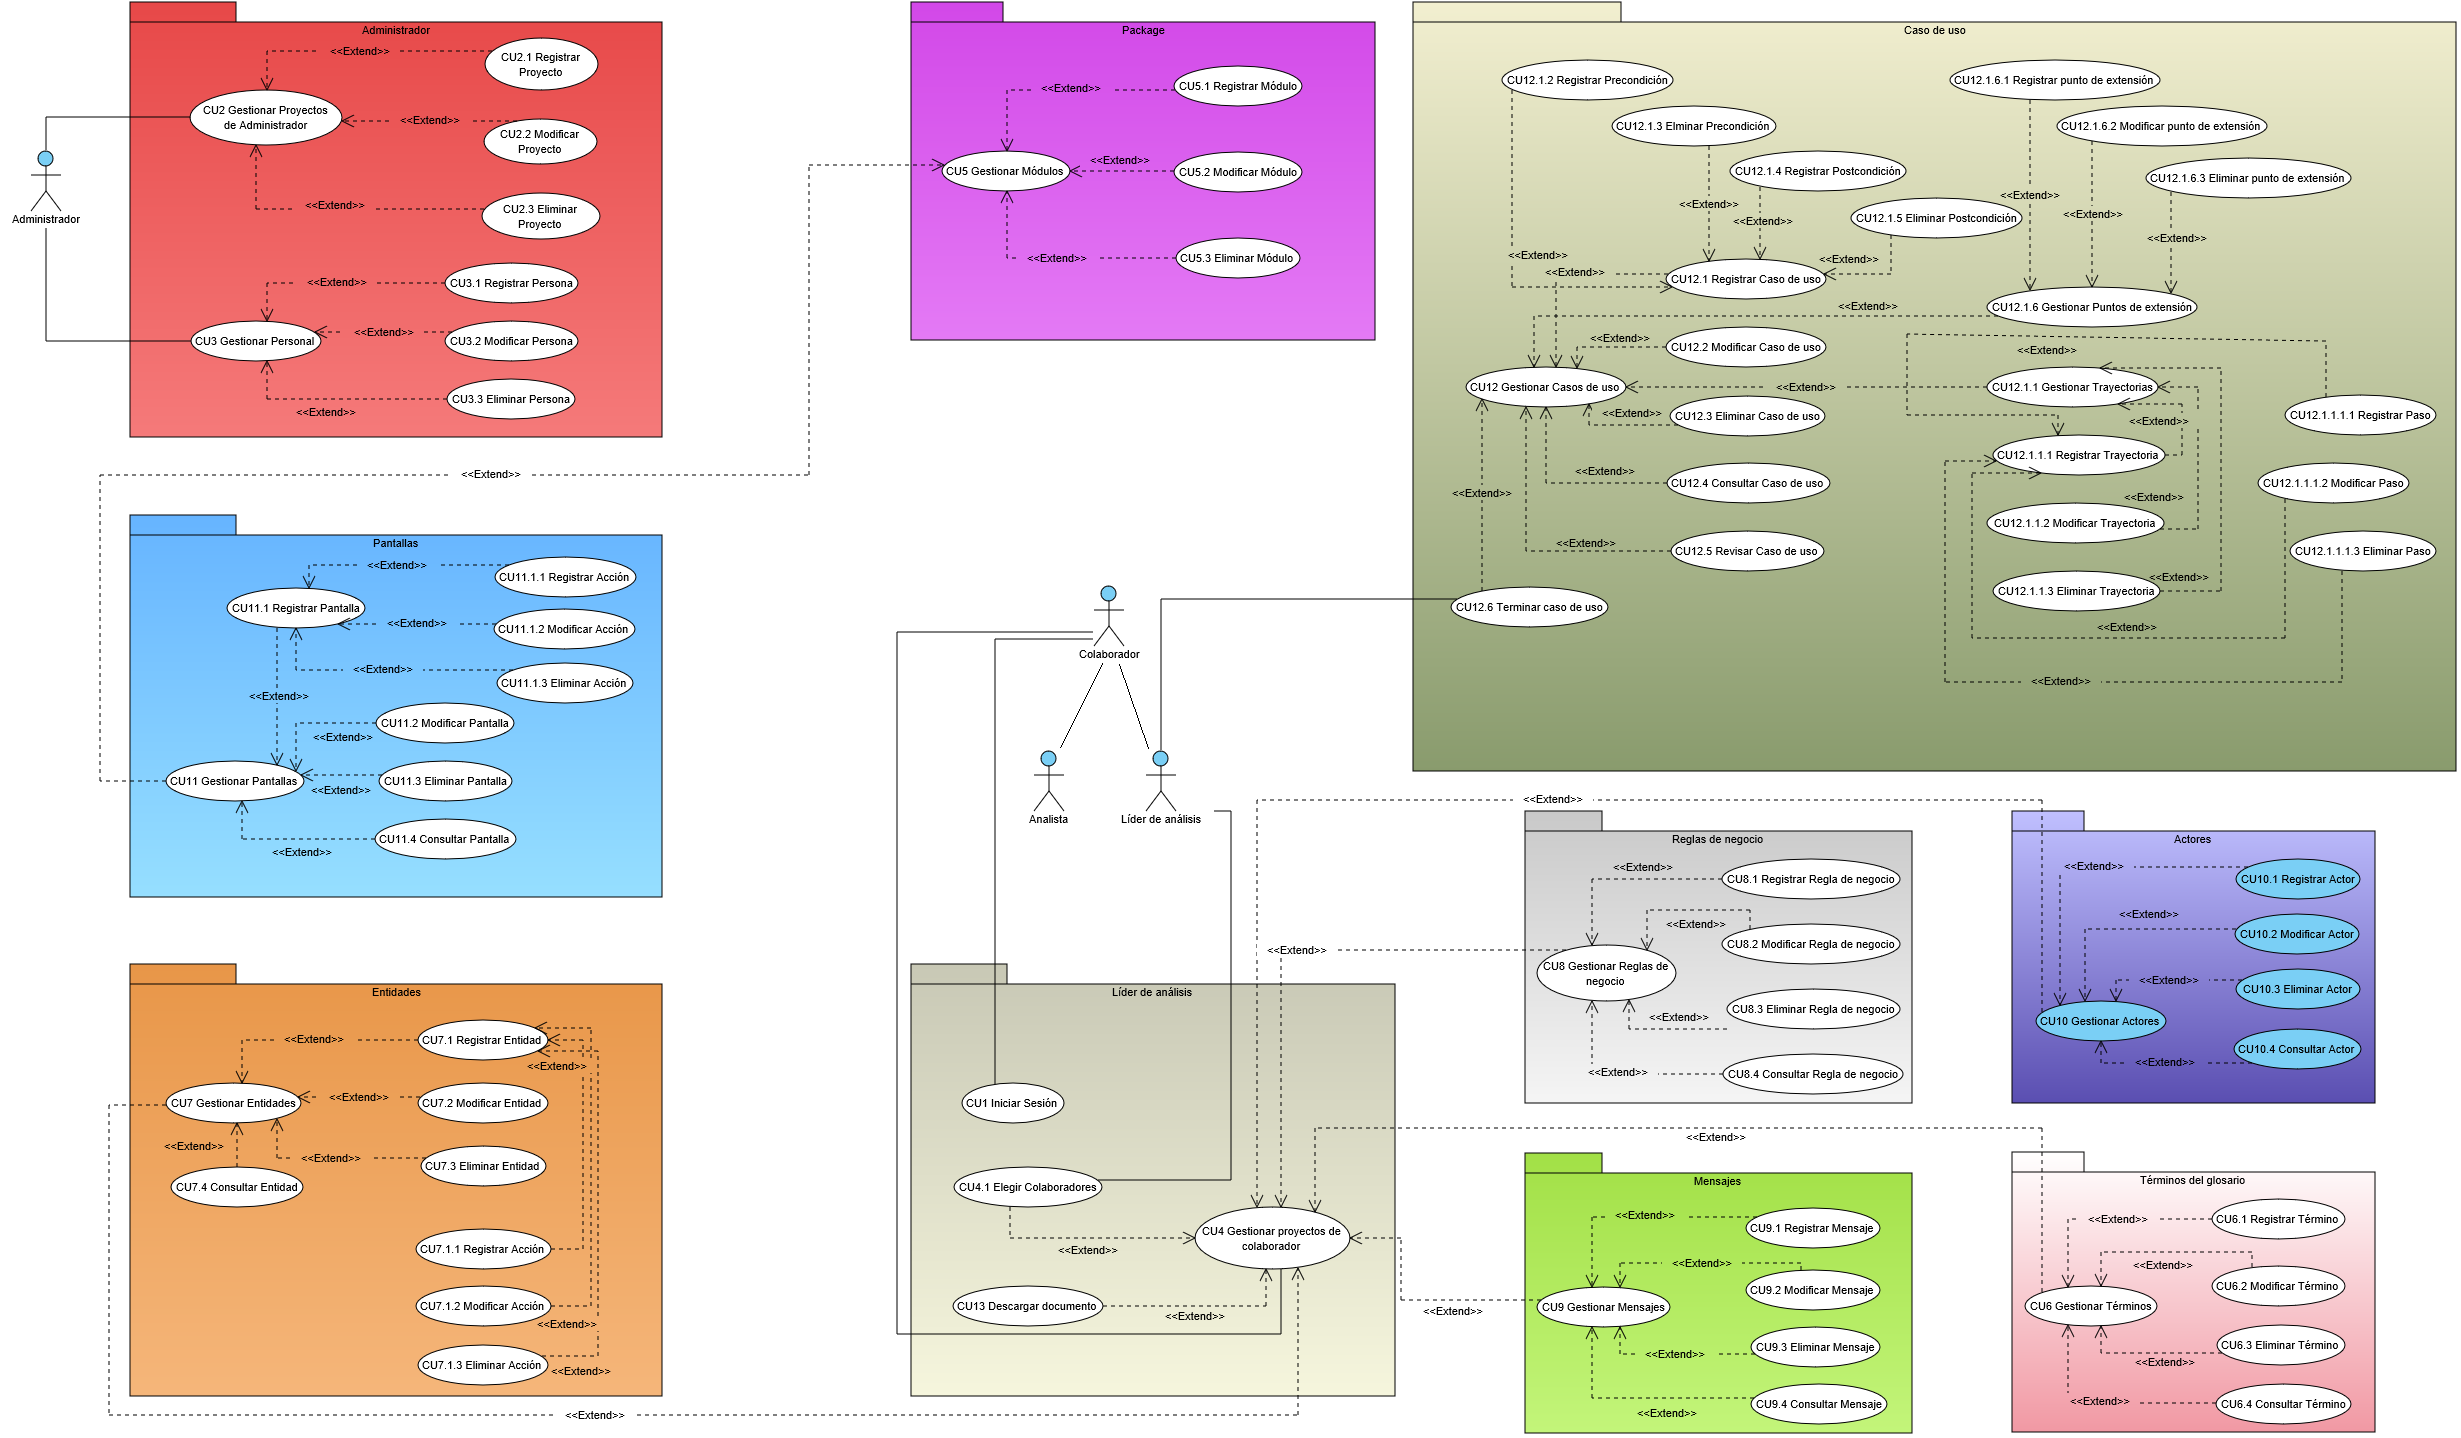
\includegraphics[angle=0,width=.95\textwidth]{images/CasosUsoTesseract}
			\caption{Casos de uso del editor}
			\label{fig:CasosUsoTesseract}
		\end{center}
	\end{figure}
\newpage

La figura \ref{fig:moduloAdmin} muestra los casos de uso del administrador que incluyen la gestión de proyectos y del personal.

	\begin{figure}[H]
		\begin{center}
			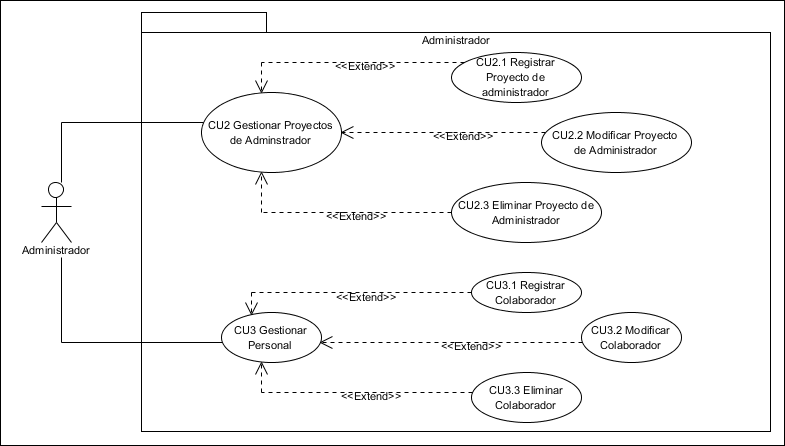
\includegraphics[angle=0,width=.80\textwidth]{images/moduloAdmin}
			\caption{Casos de uso del módulo: Administrador}
			\label{fig:moduloAdmin}
		\end{center}
	\end{figure}
\newpage
La figura \ref{fig:moduloLider} muestra los casos de uso del líder de análisis que incluyen elegir colaboradores y gestionar proyectos.

\begin{figure}[H]
	\begin{center}
		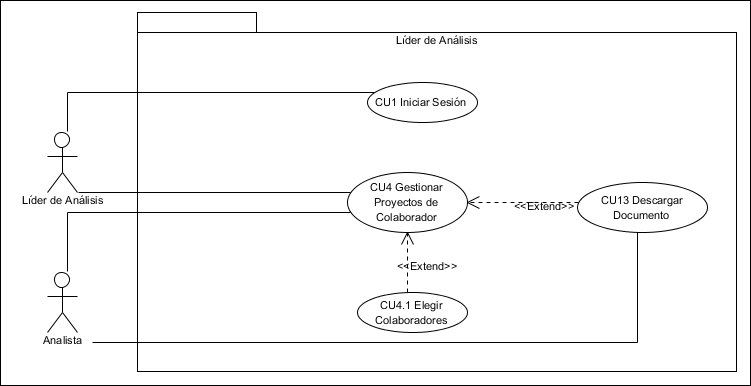
\includegraphics[angle=0,width=.70\textwidth]{images/moduloLider}
		\caption{Casos de uso del módulo: Líder de análisis}
		\label{fig:moduloLider}
	\end{center}
\end{figure}
\newpage
La figura \ref{fig:moduloModulos} muestra los casos de uso referentes a la gestión de los módulos.

\begin{figure}[H]
	\begin{center}
		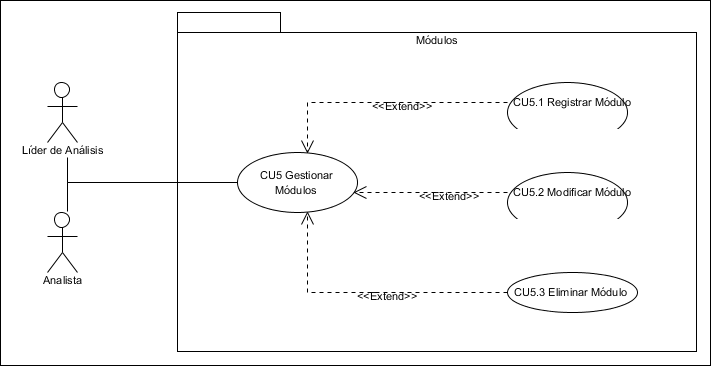
\includegraphics[angle=0,width=.70\textwidth]{images/moduloModulos}
		\caption{Casos de uso del módulo: Módulos}
		\label{fig:moduloModulos}
	\end{center}
\end{figure}
\newpage
La figura \ref{fig:moduloCU} muestra los casos de uso referentes a la gestión de los casos de uso.

\begin{figure}[H]
	\begin{center}
		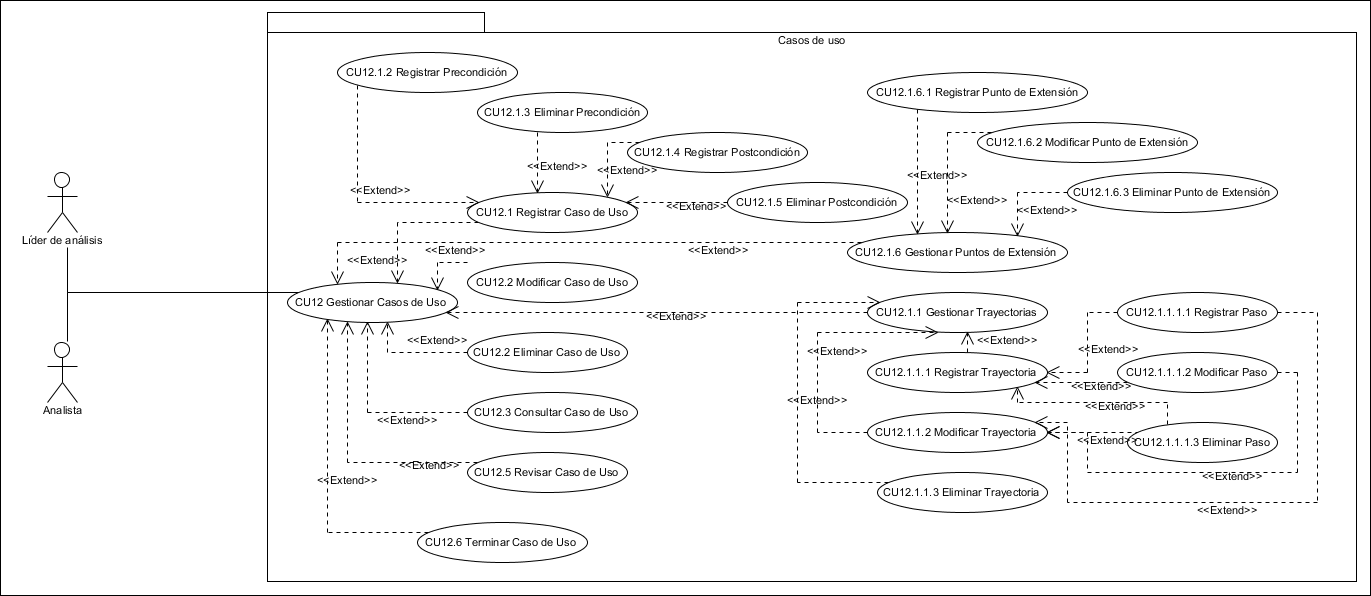
\includegraphics[angle=0,width=.70\textwidth]{images/moduloCU}
		\caption{Casos de uso del módulo: Casos de uso}
		\label{fig:moduloCU}
	\end{center}
\end{figure}
\newpage
La figura \ref{fig:moduloIU} muestra los casos de uso referentes a la gestión de las pantallas y las acciones de estas.

\begin{figure}[H]
	\begin{center}
		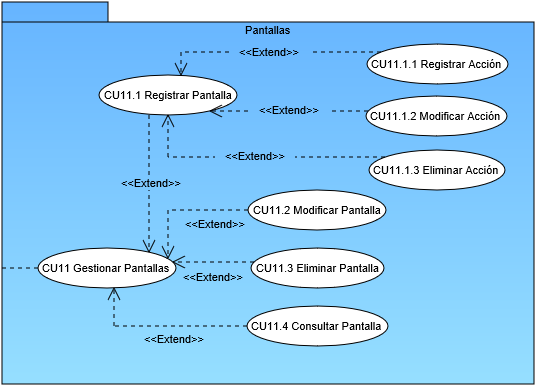
\includegraphics[angle=0,width=.70\textwidth]{images/moduloIU}
		\caption{Casos de uso del módulo: Pantallas}
		\label{fig:moduloIU}
	\end{center}
\end{figure}
\newpage
La figura \ref{fig:moduloEntidades} muestra los casos de uso referentes a la gestión de las entidades y atributos que las describen.

\begin{figure}[H]
	\begin{center}
		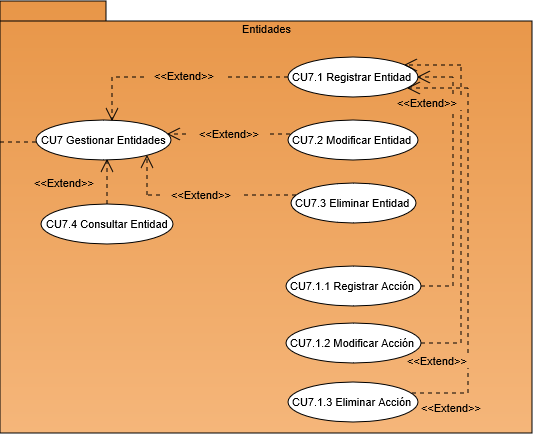
\includegraphics[angle=0,width=.70\textwidth]{images/moduloEntidades}
		\caption{Casos de uso del módulo: Entidades}
		\label{fig:moduloEntidades}
	\end{center}
\end{figure}
\newpage
La figura \ref{fig:moduloBR} muestra los casos de uso referentes a la gestión de las reglas de negocio.

\begin{figure}[H]
	\begin{center}
		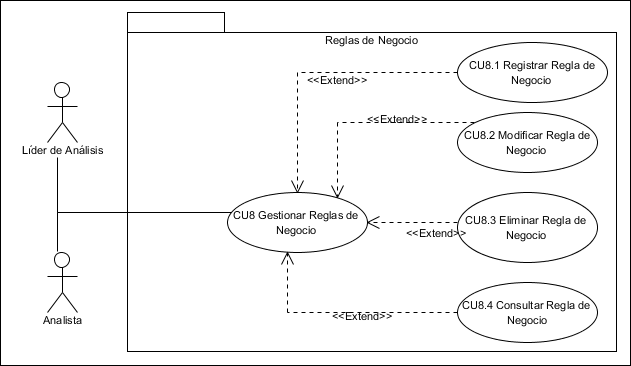
\includegraphics[angle=0,width=.70\textwidth]{images/moduloBR}
		\caption{Casos de uso del módulo: Reglas de negocio}
		\label{fig:moduloBR}
	\end{center}
\end{figure}
\newpage
La figura \ref{fig:moduloMSG} muestra los casos de uso referentes a la gestión de los mensajes.

\begin{figure}[H]
	\begin{center}
		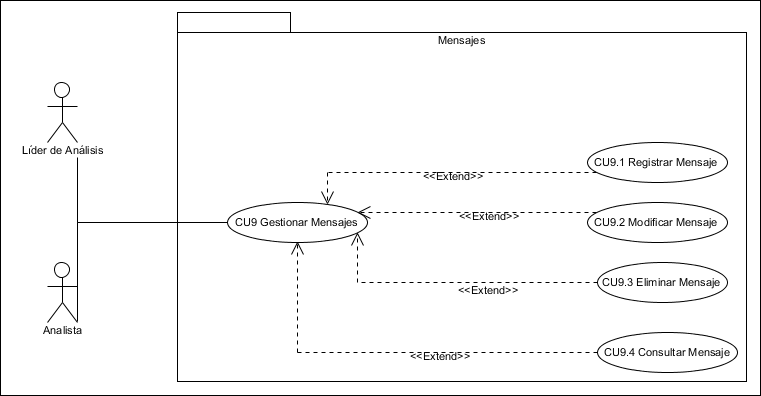
\includegraphics[angle=0,width=.70\textwidth]{images/moduloMSG}
		\caption{Casos de uso del módulo: Mensajes}
		\label{fig:moduloMSG}
	\end{center}
\end{figure}
\newpage
La figura \ref{fig:moduloActores} muestra los casos de uso referentes a la gestión de los Actores.

\begin{figure}[H]
	\begin{center}
		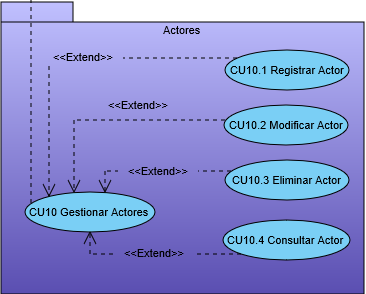
\includegraphics[angle=0,width=.70\textwidth]{images/moduloActores}
		\caption{Casos de uso del módulo: Actores}
		\label{fig:moduloActores}
	\end{center}
\end{figure}
\newpage
La figura \ref{fig:moduloGLS} muestra los casos de uso referentes a la gestión de los términos del glosario.

\begin{figure}[H]
	\begin{center}
		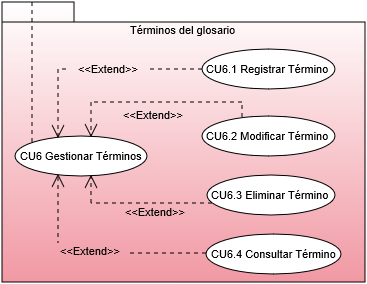
\includegraphics[angle=0,width=.70\textwidth]{images/moduloGLS}
		\caption{Casos de uso del módulo: Términos del glosario}
		\label{fig:moduloGLS}
	\end{center}
\end{figure}

	\begin{UseCase}{CU1}{Iniciar sesión}{
			
        En el inicio de sesión se controla el acceso a las distintas funciones del sistema de acuerdo con el rol asignado a un actor y mediante la entrada de datos como lo son el correo electrónico y contraseña. Tesseract define los siguientes roles con las siguientes características:
			
		 \begin{enumerate}
         \item\hyperlink{admin}{Administrador}: Actor único, encargado de  registrar los proyectos y al personal de la organización. 
         \item\hyperlink{jefe}{Líder de proyecto}: Encargado de dirigir y coordinar el proyecto en desarrollo. Asignado desde el registro del proyecto. 
         \item\hyperlink{analista}{Analista} Encargado de documentar los elementos que componen el proyecto y validar los requerimientos del software. Asignado desde el registro del proyecto. \\
         \end{enumerate}

	}
		\UCitem{Versión}{\color{Gray}0.1}
		\UCitem{Actor}{\hyperlink{jefe}{Líder de proyecto}, \hyperlink{analista}{Analista}, \hyperlink{admin}{Administrador}}
		\UCitem{Propósito}{Iniciar sesión en el sistema.}
		\UCitem{Entradas}{\begin{itemize}
				\item \cdtRef{colaboradorEntidad:correoColaborador}{Correo}: Se escribe desde el teclado
				\item \cdtRef{colaboradorEntidad:passColaborador}{Contraseña}: Se escribe desde el teclado
		\end{itemize}}
		\UCitem{Salidas}{Ninguna}
		\UCitem{Precondiciones}{Interna: Que el actor se encuentre registrado en el sistema.}
		\UCitem{Postcondiciones}{El actor podrá hacer uso del sistema dependiendo del rol que tenga.}
		\UCitem{Errores}{\begin{itemize}
		\item \cdtIdRef{MSG4}{Dato Obligatorio}: Se muestra en la pantalla \IUref{IU1}{Iniciar Sesión} cuando no se ha ingresado un dato marcado como obligatorio.
		\item \cdtIdRef{MSG6}{Longitud inválida}: Se muestra en la pantalla \IUref{IU1}{Iniciar Sesión} cuando se ha excedido la longitud de alguno de los campos.
		\item \cdtIdRef{MSG29}{Formato incorrecto}: Se muestra en la pantalla \IUref{IU1}{Iniciar Sesión} cuando el tipo de dato ingresado no cumple con el tipo de dato solicitado en el campo.
		\item \cdtIdRef{MSG23}{Correo electrónico y/o contraseña incorrectos}: Se muestra en la pantalla \IUref{IU1}{Iniciar Sesión} cuando el correo electrónico y/o la contraseña ingresada son incorrectos.
		\end{itemize}
		}
		\UCitem{Tipo}{Caso de uso primario}
	\end{UseCase}
%--------------------------------------
	\begin{UCtrayectoria}
		\UCpaso[\UCactor] Solicita ingresar al sistema a través de la URL correspondiente al proyecto.
		\UCpaso[\UCsist] Muestra la pantalla \IUref{IU1}{Iniciar Sesión}.
		\UCpaso[\UCactor] Ingresa los datos solicitados. \label{P3}
		\UCpaso[\UCactor] Oprime el botón \IUbutton{Aceptar}.
		\UCpaso[\UCsist] Verifica que no se haya omitido ningún campo marcado como obligatorio con base en la regla de negocio \BRref{RN8}{Datos Obligatorios}. \hyperlink{CU1:TAA}{[Trayectoria A]}
		\UCpaso[\UCsist] Verificar que los datos ingresados cumpla con la longitud correcta, con base en la regla de negocio \BRref{RN37}{Longitud de datos}. \hyperlink{CU1:TAB}{[Trayectoria B]}
		\UCpaso[\UCsist] Verifica que los datos cumplan con el formato y el tipo de dato requerido, con base en la regla de negocio \BRref{RN7}{Información correcta}. \hyperlink{CU1:TAC}{[Trayectoria C]}
		\UCpaso[\UCsist] Verifica que el actor se encuentre registrado en el sistema. \hyperlink{CU1:TAD}{[Trayectoria D]}
		\UCpaso[\UCsist] Verifica que la contraseña ingresada corresponda con la del usuario. \hyperlink{CU1:TAE}{[Trayectoria E]}
		\UCpaso[\UCsist] Obtiene todos los roles que tiene asociado el usuario con base a la regla de negocio \BRref{RN39}{Roles del sistema}.
		\UCpaso[\UCsist] Muestra la pantalla emergente \IUref{IU1.1}{Elegir Rol} con los roles asociados al usuario.
		\UCpaso[\UCactor] Selecciona el rol con el que iniciar sesión.
		\UCpaso[\UCactor] Presiona el botón aceptar.
		\UCpaso[\UCsist] Inicia sesión con el rol seleccionado.
		\UCpaso[\UCsist] Muestra la pantalla del rol correspondiente.
	\end{UCtrayectoria}		
%--------------------------------------
		\hypertarget{CU1:TAA}{\textbf{Trayectoria alternativa A}}\\
		\noindent \textbf{Condición:} El actor no ingresó uno o más campos obligatorios.
		\begin{enumerate}
			\UCpaso[\UCsist] Muestra el mensaje \cdtIdRef{MSG4}{Dato Obligatorio} y señala el campo que presenta el error en la pantalla \IUref{IU1}{Iniciar Sesión}.
			\UCpaso[\UCactor] Regresa al paso \ref{P3} de la Trayectoria Principal.
			\item[- -] - - {\em {Fin de la trayectoria}}.%
		\end{enumerate}

%--------------------------------------

		\hypertarget{CU1:TAB}{\textbf{Trayectoria alternativa B}}\\
		\noindent \textbf{Condición:} El actor ingresó un dato con un número de caracteres fuera del rango permitido.
		\begin{enumerate}
	\UCpaso[\UCsist] Muestra el \cdtIdRef{MSG6}{Longitud inválida} señalando el campo que presenta el error en la pantalla \IUref{IU1}{Iniciar Sesión}.
	\UCpaso[\UCactor] Regresa al paso \ref{P3} de la Trayectoria Principal.
	\item[- -] - - {\em {Fin de la trayectoria}}.
\end{enumerate}
%--------------------------------------
		\hypertarget{CU1:TAC}{\textbf{Trayectoria alternativa C}}\\
		\noindent \textbf{Condición:} El actor ingresó un dato con un formato o tipo de dato incorrecto.
	\begin{enumerate}
		\UCpaso[\UCsist] Muestra el mensaje \cdtIdRef{MSG29}{Formato incorrecto} señalando el campo que presenta el error en la pantalla \IUref{IU1}{Iniciar sesión}.
		\UCpaso Regresa al paso \ref{P3} de la trayectoria principal.
		\item[- -] - - {\em {Fin de la trayectoria}}.
	\end{enumerate}

%--------------------------------------
		\hypertarget{CU1:TAD}{\textbf{Trayectoria alternativa D}}\\
		\noindent \textbf{Condición:} El actor un correo que no se encuentra registrado en el sistema.
		\begin{enumerate}
	\UCpaso[\UCsist] Muestra el mensaje \cdtIdRef{MSG23}{Correo electrónico y/o contraseña incorrectos} en la pantalla \IUref{IU1}{Iniciar Sesión} notificando que los datos ingresados son incorrectos.
	\UCpaso[\UCactor] Regresa al paso \ref{P3} de la Trayectoria Principal.
	\item[- -] - - {\em {Fin de la trayectoria}}.
\end{enumerate}

%--------------------------------------
\hypertarget{CU1:TAE}{\textbf{Trayectoria alternativa E}}\\
\noindent \textbf{Condición:} El actor ingresó una contraseña que no corresponde al correo ingresado.
\begin{enumerate}
	\UCpaso[\UCsist] Muestra el mensaje \cdtIdRef{MSG23}{Correo electrónico y/o contraseña incorrectos} en la pantalla \IUref{IU1}{Iniciar Sesión} notificando que los datos ingresados son incorrectos.
	\UCpaso[\UCactor] Regresa al paso \ref{P3} de la Trayectoria Principal.
	\item[- -] - - {\em {Fin de la trayectoria}}.
\end{enumerate}

	\begin{UseCase}{CU2}{Gestionar proyectos de Administrador}{
			
		Permite al \hyperlink{admin}{Administrador} realizar las acciones necesarias para controlar los proyectos que han sido previamente registrados en el sistema, como lo son visualizar el listado de los proyectos, registrar un nuevo proyecto, modificarlo o eliminarlo.
		
		La gestión está disponible en cualquier estado en el que se encuentre el proyecto con base en el  \hyperlink{edoProy}{Modelo de estados del proyecto}.
				
	}
		\UCitem{Versión}{\color{Gray}0.1}
		\UCitem{Actor}{\hyperlink{admin}{Administrador}}
		\UCitem{Propósito}{Proporcionar al actor un mecanismo para llevar el control de los proyectos.}
		\UCitem{Entradas}{Ninguna}
		\UCitem{Salidas}{\begin{itemize}
				\item \hyperlink{proyectoEntidad}{Proyecto}: Tabla que muestra la \cdtRef{proyectoEntidad:claveProyecto}{clave}, \cdtRef{proyectoEntidad:nombreProyecto}{nombre} y el \cdtRef{proyectoEntidad:liderProyecto}{Líder de Proyecto} de todos los proyectos existentes.
		\end{itemize}}
		\UCitem{Destino}{Pantalla}
		\UCitem{Precondiciones}{
			\begin{itemize}
				\item Que el usuario haya iniciado sesión como \hyperlink{admin}{Administrador}.
			\end{itemize}	
		}
		\UCitem{Postcondiciones}{Ninguna}
		\UCitem{Errores}{\begin{itemize}
		\item \cdtIdRef{MSG2}{No existe información}: Se muestra en la pantalla \IUref{IU2}{Gestionar proyectos de Administrador} cuando no existen proyectos registrados
		\end{itemize}
		}
		\UCitem{Tipo}{Caso de uso primario}
	\end{UseCase}
%--------------------------------------
	\begin{UCtrayectoria}
		\UCpaso[\UCactor] Solicita gestionar los proyectos presionando la opción ''Proyectos'' del menú \IUref{MN1}{Menú de Administrador}.
		\UCpaso[\UCsist] Obtiene la información de los proyectos registrados en cualquier estado. \hyperlink{CU2:TAA}{[Trayectoria A]}
		\UCpaso[\UCsist] Ordena los proyectos alfabéticamente.
		\UCpaso[\UCsist] Muestra la información de los proyectos en la pantalla \IUref{IU2}{Gestionar proyectos de Administrador}. \label{P3}
		\UCpaso[\UCactor] Gestiona los proyectos a través de los botones: \IUbutton{Registrar}, \editar  y \eliminar. 
	\end{UCtrayectoria}		
%--------------------------------------
	\hypertarget{CU2:TAA}{\textbf{Trayectoria alternativa A}}\\
\noindent \textbf{Condición:} No existen registros de proyectos.
\begin{enumerate}
	\UCpaso[\UCsist] Muestra el mensaje \cdtIdRef{MSG2}{No existe información} en la pantalla \IUref{IU2}{Gestionar proyectos de Administrador} para indicar que no hay registros de proyectos para mostrar.
	\UCpaso[\UCactor] Gestiona los proyectos a través del botón: \IUbutton{Registrar}.
	\item[- -] - - {\em {Fin del caso de uso}}.%
\end{enumerate}
%--------------------------------------

\subsubsection{Puntos de extensión}

\UCExtenssionPoint{El actor requiere registrar un proyecto.}{Paso \ref{P3} de la trayectoria principal.}{\UCref{CU2.1}{Registrar Proyecto}}
\UCExtenssionPoint{El actor requiere modificar un proyecto.}{Paso \ref{P3} de la trayectoria principal.}{\UCref{CU2.2}{Modificar Proyecto}}
\UCExtenssionPoint{El actor requiere eliminar un proyecto.}{Paso \ref{P3} de la trayectoria principal.}{\UCref{CU2.3}{Eliminar Proyecto}}

	\begin{UseCase}{CU2.1}{Registrar proyecto}{
			Permite al {\hyperlink{admin}{Administrador}} registrar la información general de un proyecto en el sistema, dicha información está comprendida por: una \cdtRef{proyectoEntidad:claveProyecto}{clave}, un \cdtRef{proyectoEntidad:nombreProyecto}{nombre} (como medio de identificación), una breve \cdtRef{proyectoEntidad:descripcionProyecto}{descripción} (para definir objetivos y características generales) , la estimación del tiempo que tomará desarrollar el proyecto estableciendo una \cdtRef{proyectoEntidad:fechaIPProyecto}{fecha de inicio programada} y una  \cdtRef{proyectoEntidad:fechaFinPProyecto}{fecha de término programada}, \cdtRef{proyectoEntidad:contraparteProyecto}{contraparte} (en donde se específican los clientes del proyecto o partes interesadas) , el   \cdtRef{proyectoEntidad:presupuestoProyecto}{presupuesto} (en donde se establece el monto calculado del costo del proyecto), el \cdtRef{proyectoEntidad:estadoProyecto}{estado} del proyecto (al momento de registrarlo solo puede ser: En negociación o Iniciado) y por último el \cdtRef{proyectoEntidad:liderProyecto}{líder} (persona encargada de ejecutar las actividades de asociación de colaboradores al proyecto, así como las de terminar, revisar y liberar casos de uso). 
	}
		\UCitem{Versión}{\color{Gray}0.1}
		\UCitem{Actor}{\hyperlink{admin}{Administrador}}
		\UCitem{Propósito}{Registrar la información de un proyecto.}
		\UCitem{Entradas}{
		\begin{itemize}
			\item \cdtRef{proyectoEntidad:claveProyecto}{Clave:} Se escribe desde el teclado.
			\item \cdtRef{proyectoEntidad:nombreProyecto}{Nombre:} Se escribe desde el teclado.
			\item \cdtRef{proyectoEntidad:fechaIProyecto}{Fecha de inicio:} Se selecciona de un calendario.
			\item \cdtRef{proyectoEntidad:fechaFinProyecto}{Fecha de término:} Se selecciona de un calendario.
			\item \cdtRef{proyectoEntidad:fechaIPProyecto}{Fecha de inicio programada:} Se selecciona de un calendario.
			\item \cdtRef{proyectoEntidad:fechaFinPProyecto}{Fecha de término programada:} Se selecciona de un calendario.
			\item \cdtRef{proyectoEntidad:liderProyecto}{Líder del Proyecto:} Se selecciona de una lista.
			\item \cdtRef{proyectoEntidad:descripcionProyecto}{Descripción:} Se escribe desde el teclado.
			\item \cdtRef{proyectoEntidad:contraparteProyecto}{Contraparte} Se escribe desde el teclado.
			\item \cdtRef{proyectoEntidad:presupuestoProyecto}{Presupuesto:} Se escribe desde el teclado.
			\item \hyperlink{tEdoProy}{Estado del Proyecto:} Se selecciona de un lista.
		\end{itemize}	
		}
		\UCitem{Salidas}{\begin{itemize}
				\item \cdtIdRef{MSG1}{Operación exitosa}: Se muestra en la pantalla \IUref{IU2}{Gestionar proyectos de Administrador} para indicar que el registro fue exitoso.
		\end{itemize}}
		\UCitem{Destino}{Pantalla}
		\UCitem{Precondiciones}{
		\begin{itemize}
			\item Interna: Que exista al menos un colaborador registrado.
			\item Interna: Que exista información referente a los estados del proyecto.
		\end{itemize}
		}
		\UCitem{Postcondiciones}{
		\begin{itemize}
			\item Interna: Se registrará un proyecto en el sistema.
			\item Interna: Se podrán gestionar los Términos del glosario, Entidades, Reglas de negocio, Mensajes y Actores.
		\end{itemize}
		}
		\UCitem{Errores}{\begin{itemize}
		\item \cdtIdRef{MSG4}{Dato obligatorio}: Se muestra en la pantalla \IUref{IU2.1}{Registrar proyecto} cuando no se ha ingresado un dato marcado como obligatorio.
		\item \cdtIdRef{MSG29}{Formato incorrecto}: Se muestra en la pantalla \IUref{IU2.1}{Registrar proyecto} cuando el tipo de dato ingresado no cumple con el tipo de dato solicitado en el campo.
		\item \cdtIdRef{MSG6}{Longitud inválida}: Se muestra en la pantalla \IUref{IU2.1}{Registrar proyecto} cuando se ha excedido la longitud de alguno de los campos.
		\item \cdtIdRef{MSG7}{Registro repetido}: Se muestra en la pantalla \IUref{IU2.1}{Registrar proyecto} cuando se registre un proyecto con un nombre o clave que ya se encuentra registrado en el sistema.
		\item \cdtIdRef{MSG12}{Ha ocurrido un error}: Se muestra en la pantalla \IUref{IU2}{Gestionar proyectos de Administrador} cuando no exista información de los estados de un proyecto.
		\item \cdtIdRef{MSG17}{Falta información}: Se muestra en la pantalla \IUref{IU2}{Gestionar proyectos de Administrador} cuando no existan colaboradores registrados.
		\item \cdtIdRef{MSG26}{Orden de fechas}: Se muestra en la pantalla \IUref{IU2.1}{Registrar proyecto} cuando el actor ingrese fechas de término que no son posteriores a las fechas
		de inicio correspondientes.
		\end{itemize}
		}
		\UCitem{Tipo}{Secundario, extiende del caso de uso \UCref{CU2}{Gestionar proyectos de Administrador}.}
	\end{UseCase}
%--------------------------------------
	\begin{UCtrayectoria}
		\UCpaso[\UCactor] Solicita registrar un proyecto oprimiendo el botón \IUbutton{Registrar} de la pantalla \IUref{IU2}{Gestionar proyectos de Administrador}.
		\UCpaso[\UCsist] Verifica que exista información referente a los estados de un proyecto, con base en la regla de negocio \BRref{RN20}{Verificación de catálogos}. \hyperlink{CU2-1:TAA}{[Trayectoria A]}
		\UCpaso[\UCsist] Verifica que exista al menos un colaborador, con base en la regla de negocio \BRref{RN20}{Verificación de catálogos}. \hyperlink{CU2-1:TAB}{[Trayectoria B]}
		\UCpaso[\UCsist] Muestra la pantalla \IUref{IU2.1}{Registrar proyecto}.
		\UCpaso[\UCactor] Ingresa la información solicitada en la pantalla. \label{CU2.1-P5}
		\UCpaso[\UCactor] Solicita guardar el proyecto oprimiendo el botón \IUbutton{Aceptar} de la pantalla \IUref{IU2.1}{Registrar proyecto}. \hyperlink{CU2-1:TAC}{[Trayectoria C]}
		\UCpaso[\UCsist] Verifica que el actor ingrese todos los campos obligatorios con base en la regla de negocio \BRref{RN8}{Datos obligatorios}. \hyperlink{CU2-1:TAD}{[Trayectoria D]}
		\UCpaso[\UCsist] Verificar que los datos ingresados cumpla con la longitud correcta, con base en la regla de negocio \BRref{RN37}{Longitud de datos}. \hyperlink{CU2-1:TAE}{[Trayectoria E]}
		\UCpaso[\UCsist] Verifica que los datos ingresados cumplan con el formato requerido, con base en la regla de negocio \BRref{RN7}{Información correcta}. \hyperlink{CU2-1:TAF}{[Trayectoria F]}
		\UCpaso[\UCsist] Verifica que la clave del proyecto no se encuentre registrada en el sistema con base en la regla de negocio \BRref{RN22}{Unicidad de la clave del Proyecto}. \hyperlink{CU2-1:TAG}{[Trayectoria G]}
		\UCpaso[\UCsist] Verifica que el nombre del proyecto no se encuentre registrado en el sistema con base en la regla de negocio \BRref{RN6}{Unicidad de nombres}. \hyperlink{CU2-1:TAH}{[Trayectoria H]}
		\UCpaso[\UCsist] Verifica que la fecha de término programada sea posterior a la fecha de inicio programada con base en la regla de negocio \BRref{RN35}{Validar Fecha}. \hyperlink{CU2-1:TAI}{[Trayectoria I]}
		\UCpaso[\UCsist] Registra la información del proyecto en el sistema
		\UCpaso[\UCsist] Muestra el mensaje \cdtIdRef{MSG1}{Operación exitosa} en la pantalla \IUref{IU2}{Gestionar proyectos de Administrador} para indicar al actor que el registro se ha realizado exitosamente.
	\end{UCtrayectoria}		
%--------------------------------------
\hypertarget{CU2-1:TAA}{\textbf{Trayectoria alternativa A}}\\
\noindent \textbf{Condición:} El catálogo de estados de un proyecto no tiene información.
\begin{enumerate}
	\UCpaso[\UCsist] Muestra el mensaje \cdtIdRef{MSG16}{Registro Necesario} en la pantalla \IUref{IU2}{Gestionar proyectos de Administrador} para indicar que no es posible realizar la operación debido a la falta de información necesaria para el sistema.
	\item[- -] - - {\em {Fin del caso de uso}}.%
\end{enumerate}

%--------------------------------------
	\hypertarget{CU2-1:TAB}{\textbf{Trayectoria alternativa B}}\\
	\noindent \textbf{Condición:} No hay ningún colaborador registrado.
	\begin{enumerate}
		\UCpaso[\UCsist] Muestra el mensaje \cdtIdRef{MSG16}{Registro necesario} en la pantalla \IUref{IU2}{Gestionar proyectos de Administrador} para indicar que no es posible realizar la operación debido a la falta de información necesaria para el sistema.
		\item[- -] - - {\em {Fin del caso de uso}}.%
	\end{enumerate}
	
%--------------------------------------
\hypertarget{CU2-1:TAC}{\textbf{Trayectoria alternativa C}}\\
\noindent \textbf{Condición:} El actor desea cancelar la operación.
\begin{enumerate}
	\UCpaso[\UCactor] Solicita cancelar la operación oprimiendo el botón \IUbutton{Cancelar} de la pantalla \IUref{IU2.1}{Registrar Proyecto}
	\UCpaso[\UCsist] Muestra la pantalla \IUref{IU2}{Gestionar proyectos de Administrador}.
	\item[- -] - - {\em {Fin del caso de uso}}.%
\end{enumerate}
%--------------------------------------	
\hypertarget{CU2-1:TAD}{\textbf{Trayectoria alternativa D}}\\
\noindent \textbf{Condición:} El actor no ingresó algún dato marcado como obligatorio.
\begin{enumerate}
	\UCpaso[\UCsist] Muestra el mensaje \cdtIdRef{MSG4}{Dato obligatorio} señalando el campo que presenta el error en la pantalla \IUref{IU2.1}{Registrar Proyecto}.
	\UCpaso Regresa al paso \ref{CU2.1-P5} de la trayectoria principal.
	\item[- -] - - {\em {Fin de la trayectoria}}.%
\end{enumerate}
%--------------------------------------
\hypertarget{CU2-1:TAE}{\textbf{Trayectoria alternativa E}}\\
\noindent \textbf{Condición:} El actor ingresó un dato con un número de caracteres fuera del rango permitido.
\begin{enumerate}
	\UCpaso[\UCsist] Muestra el mensaje \cdtIdRef{MSG6}{Longitud inválida} señalando el campo que presenta el error en la pantalla \IUref{IU2.1}{Registrar Proyecto}.
	\UCpaso Regresa al paso \ref{CU2.1-P5} de la trayectoria principal.
	\item[- -] - - {\em {Fin de la trayectoria}}.%
\end{enumerate}
%-------------------------------------
\hypertarget{CU2-1:TAF}{\textbf{Trayectoria alternativa F}}\\
\noindent \textbf{Condición:} El actor ingresó un dato con un formato de dato incorrecto.
\begin{enumerate}
	\UCpaso[\UCsist] Muestra el mensaje \cdtIdRef{MSG29}{Formato incorrecto} señalando el campo que presenta el error en la pantalla \IUref{IU2.1}{Registrar Proyecto}.
	\UCpaso Regresa al paso \ref{CU2.1-P5} de la trayectoria principal.
	\item[- -] - - {\em {Fin de la trayectoria}}.
\end{enumerate}
%--------------------------------------
\hypertarget{CU2-1:TAG}{\textbf{Trayectoria alternativa G}}\\
\noindent \textbf{Condición:} El actor ingresó una clave de proyecto que ya existe dentro del sistema.
\begin{enumerate}
	\UCpaso[\UCsist] Muestra el mensaje \cdtIdRef{MSG7}{Registro repetido} señalando el campo que presenta la duplicidad en la pantalla \IUref{IU2.1}{Registrar Proyecto}.
	\UCpaso Regresa al paso \ref{CU2.1-P5} de la trayectoria principal.
	\item[- -] - - {\em {Fin de la trayectoria}}.
\end{enumerate}
%--------------------------------------	
\hypertarget{CU2-1:TAH}{\textbf{Trayectoria alternativa H}}\\
\noindent \textbf{Condición:} El actor ingresó un nombre de proyecto que ya existe dentro del sistema.
\begin{enumerate}
	\UCpaso[\UCsist] Muestra el mensaje \cdtIdRef{MSG7}{Registro repetido} señalando el campo que presenta la duplicidad en la pantalla \IUref{IU2.1}{Registrar Proyecto}.
	\UCpaso Regresa al paso \ref{CU2.1-P5} de la trayectoria principal.
	\item[- -] - - {\em {Fin de la trayectoria}}.
\end{enumerate}
%--------------------------------------
\hypertarget{CU2-1:TAI}{\textbf{Trayectoria alternativa I}}\\
\noindent \textbf{Condición:} La fecha de termino programada es menor a la fecha de inicio programada.
\begin{enumerate}
	\UCpaso[\UCsist] Muestra el mensaje \cdtIdRef{MSG26}{Orden de fechas} en el campo de fecha de término programada en la pantalla \IUref{IU2.1}{Registrar Proyecto}.
	\UCpaso Regresa al paso \ref{CU2.1-P5} de la trayectoria principal.
	\item[- -] - - {\em {Fin de la trayectoria}}.
\end{enumerate}
	\begin{UseCase}{CU2.2}{Modificar proyecto de Administrador}{
			Cuando se ha registrado un nuevo \hyperlink{proyectoEntidad}{Proyecto} y se requiere modificar su información, el sistema mostrará al {\hyperlink{admin}{Administrador}} un formulario mediante el cual podrá actualizar cualquiera de los datos previamente registrados.\\
			Debe considerarse que la \cdtRef{proyectoEntidad:claveProyecto}{Clave} y el \cdtRef{proyectoEntidad:nombreProyecto}{Nombre del proyecto} son únicos, por lo que no será posible repetir esta información con la de otros proyectos registrados.\\
			Una vez registrado el \hyperlink{proyectoEntidad}{Proyecto}, es posible modificar su \cdtRef{proyectoEntidad:estadoProyecto}{estado} a: Iniciado, Negociación y también a Terminado.
	}
		\UCitem{Actor}{\hyperlink{admin}{Administrador}}
		\UCitem{Propósito}{Modificar la información de un proyecto.}
		\UCitem{Entradas}{
		\begin{itemize}
			\item \cdtRef{proyectoEntidad:claveProyecto}{Clave del proyecto:} Se escribe desde el teclado.
			\item \cdtRef{proyectoEntidad:nombreProyecto}{Nombre del proyecto:} Se escribe desde el teclado.
			\item \cdtRef{proyectoEntidad:fechaIProyecto}{Fecha de inicio:} Se selecciona de un calendario.
			\item \cdtRef{proyectoEntidad:fechaFinProyecto}{Fecha de término:} Se selecciona de un calendario.
			\item \cdtRef{proyectoEntidad:fechaIPProyecto}{Fecha de inicio programada:} Se selecciona de un calendario.
			\item \cdtRef{proyectoEntidad:fechaFinPProyecto}{Fecha de término programada:} Se selecciona de un calendario.
			\item \cdtRef{proyectoEntidad:liderProyecto}{Líder del Proyecto:} Se selecciona de una lista.
			\item \cdtRef{proyectoEntidad:descripcionProyecto}{Descripción del proyecto:} Se escribe desde el teclado.
			\item \cdtRef{proyectoEntidad:contraparteProyecto}{Contraparte} Se escribe desde el teclado.
			\item \cdtRef{proyectoEntidad:presupuestoProyecto}{Presupuesto del proyecto:} Se escribe desde el teclado.
			\item \hyperlink{tEdoProy}{Estado del Proyecto:} Se selecciona de un lista.
		\end{itemize}	
		}
		\UCitem{Salidas}{\begin{itemize}
				\item \cdtRef{proyectoEntidad:claveProyecto}{Clave del proyecto:} Lo obtiene el sistema.
				\item \cdtRef{proyectoEntidad:nombreProyecto}{Nombre del proyecto:} Lo obtiene el sistema.
				\item \cdtRef{proyectoEntidad:fechaIProyecto}{Fecha de inicio:} Lo obtiene el sistema.
				\item \cdtRef{proyectoEntidad:fechaFinProyecto}{Fecha de término:} Lo obtiene el sistema.
				\item \cdtRef{proyectoEntidad:fechaIPProyecto}{Fecha de inicio programada:} Lo obtiene el sistema.
				\item \cdtRef{proyectoEntidad:fechaFinPProyecto}{Fecha de término programada:} Lo obtiene el sistema.
				\item \cdtRef{proyectoEntidad:liderProyecto}{Líder del Proyecto:} Lo obtiene el sistema.
				\item \cdtRef{proyectoEntidad:descripcionProyecto}{Descripción del proyecto:} Lo obtiene el sistema.
				\item \cdtRef{proyectoEntidad:contraparteProyecto}{Contraparte} Lo obtiene el sistema.
				\item \cdtRef{proyectoEntidad:presupuestoProyecto}{Presupuesto del proyecto:} Lo obtiene el sistema.
				\item \hyperlink{tEdoProy}{Estado del Proyecto:} Lo obtiene el sistema.
				\item \cdtIdRef{MSG1}{Operación exitosa}: Se muestra en la pantalla \IUref{IU2}{Gestionar proyectos de Administrador} para indicar que el registro fue exitoso.
		\end{itemize}}
		\UCitem{Precondiciones}{
			\begin{itemize}
				\item Que el proyecto se encuentre en estado ''En negociación'' o ''Iniciado''.
				\item Que exista al menos un proyecto registrado en el sistema
				\item Que exista al menos un colaborador registrado.
				\item Que exista información dentro del catálogo ''estados un proyecto''.
			\end{itemize}
		}
		\UCitem{Postcondiciones}{
			Se modificará la información del proyecto en el sistema.
		}
		\UCitem{Errores}{\begin{itemize}
		\item \cdtIdRef{MSG4}{Dato obligatorio}: Se muestra en la pantalla \IUref{IU2.2}{Modificar proyecto} cuando no se ha ingresado un dato marcado como obligatorio.
		\item \cdtIdRef{MSG5}{Formato incorrecto}: Se muestra en la pantalla \IUref{IU2.2}{Modificar proyecto} cuando el tipo de dato ingresado no cumple con el tipo de dato solicitado en
		el campo.
		\item \cdtIdRef{MSG6}{Longitud inválida}: Se muestra en la pantalla \IUref{IU2.2}{Modificar proyecto} cuando se ha excedido la longitud de alguno de los campos.
		\item \cdtIdRef{MSG7}{Registro repetido}: Se muestra en la pantalla \IUref{IU2.2}{Modificar proyecto} cuando se registre un proyecto con un nombre o clave que ya exista.
		\item \cdtIdRef{MSG29}{Los catálogos nos contienen información}: Se muestra en la pantalla \IUref{IU2}{Gestionar proyectos de Administrador} cuando no exista información en el catálogo ''estados de un proyecto''.
		\item \cdtIdRef{MSG15}{Falta información}: Se muestra en la pantalla \IUref{IU2}{Gestionar proyectos de Administrador} cuando no existan colaboradores registrados.
		\item \cdtIdRef{MSG22}{Orden de fechas}: Se muestra en la pantalla \IUref{IU2.2}{Modificar proyecto} cuando el actor ingrese fechas de término que no son posteriores a las fechas
		de inicio correspondientes.
		\end{itemize}
		}
		\UCitem{Tipo}{Secundario, extiende del caso de uso \UCref{CU2}{Gestionar proyectos de Administrador}}
	\end{UseCase}
%--------------------------------------
	\begin{UCtrayectoria}
		\UCpaso[\UCactor] Da clic en el icono \editar de la pantalla \IUref{IU2}{Gestionar proyectos de Administrador}.
		\UCpaso[\UCsist] Verifica que exista información referente a los estados de un proyecto, con base en la regla de negocio \BRref{RN20}{Verificación de catálogos}. \hyperlink{CU2-2:TAA}{[Trayectoria A]}
		\UCpaso[\UCsist] Verifica que exista al menos un colaborador, con base en la regla de negocio \BRref{RN20}{Verificación de catálogos}. \hyperlink{CU2-2:TAB}{[Trayectoria B]}
		\UCpaso[\UCsist] Obtiene la información del proyecto seleccionado.
		\UCpaso[\UCsist] Muestra la pantalla \IUref{IU2.2}{Modificar proyecto}.
		\UCpaso[\UCactor] Modifica la información del proyecto. \label{CU2.2-P5}
		\UCpaso[\UCactor] Oprime el botón \IUbutton{Aceptar}. \hyperlink{CU2-2:TAC}{[Trayectoria C]}
		\UCpaso[\UCsist] Verifica que el actor ingrese todos los campos obligatorios con base en la regla de negocio \BRref{RN8}{Datos obligatorios}. \hyperlink{CU2-2:TAD}{[Trayectoria D]}
		\UCpaso[\UCsist] Verificar que los datos ingresados cumpla con la longitud correcta, con base en la regla de negocio \BRref{RN37}{Longitud de datos}. \hyperlink{CU2-2:TAE}{[Trayectoria E]}
		\UCpaso[\UCsist] Verifica que los datos ingresados cumplan con el formato requerido, con base en la regla de negocio \BRref{RN7}{Información correcta}. \hyperlink{CU2-2:TAF}{[Trayectoria F]}
		\UCpaso[\UCsist] Verifica que la clave del proyecto no se encuentre registrada en el sistema con base en la regla de negocio \BRref{RN22}{Unicidad de la clave del Proyecto}. \hyperlink{CU2-2:TAG}{[Trayectoria G]}
		\UCpaso[\UCsist] Verifica que el nombre del proyecto no se encuentre registrado en el sistema con base en la regla de negocio \BRref{RN6}{Unicidad de nombres}. \hyperlink{CU2-2:TAH}{[Trayectoria H]}
		\UCpaso[\UCsist] Verifica que la fecha de término programada sea posterior a la fecha de inicio programada con base en la regla de negocio \BRref{RN35}{Validar Fecha}. \hyperlink{CU2-2:TAI}{[Trayectoria I]}
		\UCpaso[\UCsist] Actualiza la información del proyecto.
		\UCpaso[\UCsist] Muestra el mensaje \cdtIdRef{MSG1}{Operación exitosa} en la pantalla \IUref{IU2}{Gestionar proyectos de Administrador} para indicar al actor que la modificación se ha realizado exitosamente.
	\end{UCtrayectoria}		
%--------------------------------------
	\hypertarget{CU2-2:TAA}{\textbf{Trayectoria alternativa A}}\\
	\noindent \textbf{Condición:} El catálogo de estados de un proyecto no tiene información.
	\begin{enumerate}
		\UCpaso[\UCsist] Muestra el mensaje \cdtIdRef{MSG29}{Los catálogos nos contienen información} en la pantalla \IUref{IU2}{Gestionar proyectos de Administrador} para indicar que no es posible realizar la operación debido a la falta de información necesaria para el sistema.
		\item[- -] - - {\em {Fin del caso de uso}}.%
	\end{enumerate}
	
	%--------------------------------------
	\hypertarget{CU2-2:TAB}{\textbf{Trayectoria alternativa B}}\\
	\noindent \textbf{Condición:} No hay ningún colaborador registrado.
	\begin{enumerate}
		\UCpaso[\UCsist] Muestra el mensaje \cdtIdRef{MSG15}{Falta información} en la pantalla \IUref{IU2}{Gestionar proyectos de Administrador} para indicar que no existen colaboradores registrados.
		\item[- -] - - {\em {Fin del caso de uso}}.%
	\end{enumerate}
	
	%--------------------------------------
	\hypertarget{CU2-2:TAC}{\textbf{Trayectoria alternativa C}}\\
	\noindent \textbf{Condición:} El actor desea cancelar la operación.
	\begin{enumerate}
		\UCpaso[\UCactor] Solicita cancelar la operación oprimiendo el botón \IUbutton{Cancelar} de la pantalla \IUref{IU2.2}{Modificar Proyecto}
		\UCpaso[\UCsist] Muestra la pantalla \IUref{IU2}{Gestionar proyectos de Administrador}.
		\item[- -] - - {\em {Fin del caso de uso}}.%
	\end{enumerate}
	%--------------------------------------	
	\hypertarget{CU2-2:TAD}{\textbf{Trayectoria alternativa D}}\\
	\noindent \textbf{Condición:} El actor no ingresó algún dato marcado como obligatorio.
	\begin{enumerate}
		\UCpaso[\UCsist] Muestra el mensaje \cdtIdRef{MSG4}{Dato obligatorio} señalando el campo que presenta el error en la pantalla \IUref{IU2.2}{Modificar Proyecto}.
		\UCpaso Regresa al paso \ref{CU2.2-P5} de la trayectoria principal.
		\item[- -] - - {\em {Fin de la trayectoria}}.%
	\end{enumerate}
	%--------------------------------------
	\hypertarget{CU2-2:TAE}{\textbf{Trayectoria alternativa E}}\\
	\noindent \textbf{Condición:} El actor ingresó un dato con un número de caracteres fuera del rango permitido.
	\begin{enumerate}
		\UCpaso[\UCsist] Muestra el mensaje \cdtIdRef{MSG6}{Longitud inválida} señalando el campo que presenta el error en la pantalla \IUref{IU2.2}{Modificar Proyecto}.
		\UCpaso Regresa al paso \ref{CU2.2-P5} de la trayectoria principal.
		\item[- -] - - {\em {Fin de la trayectoria}}.%
	\end{enumerate}
	%-------------------------------------
	\hypertarget{CU2-2:TAF}{\textbf{Trayectoria alternativa F}}\\
	\noindent \textbf{Condición:} El actor ingresó un dato con un formato o tipo de dato incorrecto.
	\begin{enumerate}
		\UCpaso[\UCsist] Muestra el mensaje \cdtIdRef{MSG5}{Formato incorrecto} señalando el campo que presenta el error en la pantalla \IUref{IU2.2}{Modificar Proyecto}.
		\UCpaso Regresa al paso \ref{CU2.2-P5} de la trayectoria principal.
		\item[- -] - - {\em {Fin de la trayectoria}}.
	\end{enumerate}
	%--------------------------------------
	\hypertarget{CU2-2:TAG}{\textbf{Trayectoria alternativa G}}\\
	\noindent \textbf{Condición:} El actor ingresó una clave de proyecto que ya existe dentro del sistema.
	\begin{enumerate}
		\UCpaso[\UCsist] Muestra el mensaje \cdtIdRef{MSG7}{Registro repetido} señalando el campo que presenta la duplicidad en la pantalla \IUref{IU2.2}{Modificar Proyecto}.
		\UCpaso Regresa al paso \ref{CU2.2-P5} de la trayectoria principal.
		\item[- -] - - {\em {Fin de la trayectoria}}.
	\end{enumerate}
	%--------------------------------------	
	\hypertarget{CU2-2:TAH}{\textbf{Trayectoria alternativa H}}\\
	\noindent \textbf{Condición:} El actor ingresó un nombre de proyecto que ya existe dentro del sistema.
	\begin{enumerate}
		\UCpaso[\UCsist] Muestra el mensaje \cdtIdRef{MSG7}{Registro repetido} señalando el campo que presenta la duplicidad en la pantalla \IUref{IU2.2}{Modificar Proyecto}.
		\UCpaso Regresa al paso \ref{CU2.2-P5} de la trayectoria principal.
		\item[- -] - - {\em {Fin de la trayectoria}}.
	\end{enumerate}
	%--------------------------------------
	\hypertarget{CU2-2:TAI}{\textbf{Trayectoria alternativa I}}\\
	\noindent \textbf{Condición:} La fecha de termino programada es menor a la fecha de inicio programada.
	\begin{enumerate}
		\UCpaso[\UCsist] Muestra el mensaje \cdtIdRef{MSG22}{Orden de fechas} en el campo de fecha de término programada en la pantalla \IUref{IU2.2}{Modificar Proyecto}.
		\UCpaso Regresa al paso \ref{CU2.2-P5} de la trayectoria principal.
		\item[- -] - - {\em {Fin de la trayectoria}}.
	\end{enumerate}
	\begin{UseCase}{CU2.3}{Eliminar proyecto}{
			Este caso de uso permite al {\hyperlink{admin}{Administrador}} eliminar la información de un \hyperlink{proyectoEntidad}{Proyecto} en el sistema. \\
		Un \hyperlink{proyectoEntidad}{Proyecto} podrá ser eliminado siempre y cuando no esten asociados casos de uso a los módulos registrados.
	}
		\UCitem{Versión}{\color{Gray}0.1}
		\UCitem{Actor}{\hyperlink{admin}{Administrador}}
		\UCitem{Propósito}{Eliminar un proyecto del sistema.}
		\UCitem{Entradas}{Niguna}	
		\UCitem{Salidas}{
		\begin{itemize}
			\item \cdtIdRef{MSG1}{Operación Exitosa}: Se muestra en la pantalla \IUref{IU2}{Gestionar proyectos de Administrador} para indicar el proyecto fue eliminado correctamente.
			\item \cdtIdRef{MSG10}{Confirmar eliminación}: Se muestra para que el actor confirme la eliminación.
		\end{itemize}
		}
		\UCitem{Precondiciones}{Ninguna}
		\UCitem{Postcondiciones}{
		\begin{itemize}
			\item Se eliminará la información del proyecto en el sistema.
		\end{itemize}
		}
		\UCitem{Errores}{\begin{itemize}
		\item \cdtIdRef{MSG32}{No es posible eliminar}: Se muestra en la pantalla \IUref{IU2}{Gestionar proyectos de Adminstrador} cuando el proyecto tiene elementos asociados.
		\end{itemize}
		}
		\UCitem{Tipo}{Secundario, extiende del caso de uso \UCref{CU2}{Gestionar proyectos de Administrador}}
	\end{UseCase}
%--------------------------------------
	\begin{UCtrayectoria}
		\UCpaso[\UCactor] Solicita eliminar un proyecto oprimiendo el botón \eliminar del registro que desea eliminar de la pantalla \IUref{IU2}{Gestionar proyectos de Administrador}.
		\UCpaso[\UCsist] Muestra el mensaje \cdtIdRef{MSG10}{Confirmar eliminación} en la pantalla \IUref{IU2}{Gestionar proyectos de Administrador} con los botones \IUbutton{Aceptar} y \IUbutton{Cancelar}
		\UCpaso[\UCsist] Confirma la eliminación del proyecto oprimiendo el botón \IUbutton{Aceptar}. \hyperlink{CU2-3:TAA}{[Trayectoria A]}
		\UCpaso[\UCsist] Verifica que el proyecto pueda eliminarse, con base en la regla de negocio \BRref{RN34}{Eliminación de proyectos}. \hyperlink{CU2-3:TAB}{[Trayectoria B]}
		\UCpaso[\UCsist] Elimina el proyecto del sistema.
		\UCpaso[\UCsist] Muestra el mensaje \cdtIdRef{MSG1}{Operación exitosa} en la pantalla \IUref{IU2}{Gestionar proyectos de Administrador} para indicar al actor que se ha eliminado el registro exitosamente.
	\end{UCtrayectoria}		
%--------------------------------------	
	\hypertarget{CU2-3:TAA}{\textbf{Trayectoria alternativa A}}\\
	\noindent \textbf{Condición:} El actor desea cancelar la operación.
	\begin{enumerate}
		\UCpaso[\UCactor] Solicita cancelar la operación oprimiendo el botón \IUbutton{Cancelar} de la ventana emergente.
		\UCpaso[\UCsist] Muestra la pantalla \IUref{IU2}{Gestionar proyectos de Administrador}.
		\item[- -] - - {\em {Fin del caso de uso}}.%
	\end{enumerate}

%--------------------------------------
	\hypertarget{CU2-3:TAB}{\textbf{Trayectoria alternativa B}}\\
	\noindent \textbf{Condición:} El proyecto tiene elementos asociados.
	\begin{enumerate}
		\UCpaso[\UCsist] Muestra la pantalla \IUref{IU2}{Gestionar proyectos de Administrador} con el mensaje \cdtIdRef{MSG32}{No es posible eliminar}.
		\item[- -] - - {\em {Fin del caso de uso}}.%
	\end{enumerate}
	\begin{UseCase}{CU3}{Gestionar Personal}{
		Permite al {\hyperlink{admin}{Administrador} visualizar en una tabla, el registro de todas las personas que forman parte de la organización, así como solicitar el registro de un nuevo miembro, modificar alguno existente (con el fin de actualizar su información personal y de acceso al sistema) o eliminarlo (en caso de que la persona ya no forme parte de la compañía).\\}
	}
	\UCitem{Versión}{\color{Gray}0.1}
	\UCitem{Actor}{\hyperlink{admin}{Administrador}}
	\UCitem{Propósito}{Proporcionar al actor un mecanismo para llevar el control del personal.}
	\UCitem{Entradas}{Ninguna}
	\UCitem{Salidas}{\begin{itemize}
			\item : \cdtRef{colaboradorEntidad}{Colaborador}: Tabla que muestra \cdtRef{colaboradorEntidad:curpColaborador}{CURP}, \cdtRef{colaboradorEntidad:nombreColaborador}{Nombre}, \cdtRef{colaboradorEntidad:pApellidoColaborador}{Primer Apellido}, \cdtRef{colaboradorEntidad:sApellidoColaborador}{Segundo Apellido} de todos los registros de las personas.
			\item \cdtIdRef{MSG2}{No existe información}: Se muestra en la pantalla \IUref{IU2}{Gestionar proyectos de Administrador} cuando no existe personal registrado.
	\end{itemize}}
	\UCitem{Destino}{Pantalla}
	\UCitem{Precondiciones}{Ninguna}
	\UCitem{Postcondiciones}{Ninguna}
	\UCitem{Errores}{Ninguno}
	\UCitem{Tipo}{Caso de uso primario}
\end{UseCase}
%--------------------------------------
\begin{UCtrayectoria}
	\UCpaso[\UCactor] Solicita gestionar al personal presionando la opción ''Personal'' del menú \IUref{MN1}{Menú de Administrador}.
	\UCpaso[\UCsist] Obtiene la información del personal registrado. \hyperlink{CU3:TAA}{[Trayectoria A]}
	\UCpaso[\UCsist] Muestra la información del personal en la pantalla \IUref{IU3}{Gestionar Personal}.
	\UCpaso[\UCactor] Gestiona los proyectos a través de los botones: \IUbutton{Registrar}, \editar  y \eliminar. \label{CU3-P4}
\end{UCtrayectoria}		
%--------------------------------------
\hypertarget{CU3:TAA}{\textbf{Trayectoria alternativa A}}\\
\noindent \textbf{Condición:} No existen registros de colaboradores.
\begin{enumerate}
	\UCpaso[\UCsist] Muestra el mensaje \cdtIdRef{MSG2}{No existe información} en la pantalla \IUref{IU3}{Gestionar Personal} para indicar que no hay registros de colaboradores para mostrar.
	\item[- -] - - {\em {Fin de la trayectoria}}.%
\end{enumerate}
%--------------------------------------

\subsubsection{Puntos de extensión}

\UCExtenssionPoint{El actor requiere registrar una persona.}{Paso \ref{CU3-P4} de la trayectoria principal.}{\UCref{CU3.1}{Registrar Persona}}
\UCExtenssionPoint{El actor requiere modificar una persona.}{Paso \ref{CU3-P4} de la trayectoria principal.}{\UCref{CU3.2}{Modificar Persona}}
\UCExtenssionPoint{El actor requiere eliminar una persona.}{Paso \ref{CU3-P4} de la trayectoria principal.}{\UCref{CU3.3}{Eliminar Persona}}

	\begin{UseCase}{CU3.1}{Registrar Colaborador}{
		Permite al {\hyperlink{admin}{Administrador}} registrar la información de un colaborador en el sistema, dicho integrante podrá ser elegido como {\hyperlink{jefe}{lider de proyecto}} o {\hyperlink{analista}{analista}}.\\
		Cuando se desea registrar un nuevo miembro se le solicitará al administrador mediante un formulario el llenado de la información personal del nuevo participante así como de sus credenciales para acceder al sistema.
	}
		\UCitem{Versión}{\color{Gray}0.1}
		\UCitem{Actor}{\hyperlink{admin}{Administrador}}
		\UCitem{Propósito}{Registrar la información de una nueva Colaborador para que pueda ser asociada como colaborador de uno o varios proyetos.}
		\UCitem{Entradas}{
		\begin{itemize}
			\item \cdtRef{colaboradorEntidad:curpColaborador}{CURP}: Se escribe desde el teclado.
			\item \cdtRef{colaboradorEntidad:nombreColaborador}{Nombre}: Se escribe desde el teclado.
			\item \cdtRef{colaboradorEntidad:pApellidoColaborador}{Primer Apellido}: Se escribe desde el teclado.
			\item \cdtRef{colaboradorEntidad:sApellidoColaborador}{Segundo Apellido}: Se escribe desde el teclado.
			\item \cdtRef{colaboradorEntidad:correoColaborador}{Correo electrónico}: Se escribe desde el teclado.
			\item \cdtRef{colaboradorEntidad:passColaborador}{Contraseña}: Se escribe desde el teclado.
		\end{itemize}	
		}
		\UCitem{Salidas}{\begin{itemize}
				\item \cdtIdRef{MSG1}{Operación exitosa}: Se muestra en la pantalla \IUref{IU3}{Gestionar Colaboradores} para indicar que el registro fue exitoso.
		\end{itemize}}
		\UCitem{Precondiciones}{Ninguna}
		\UCitem{Postcondiciones}{
		\begin{itemize}
			\item Se registrará un Colaborador en el sistema.
			\item El Colaborador registrada se podrá elegir para participar en algún proyecto.
		\end{itemize}
		}
		\UCitem{Errores}{\begin{itemize}
		\item \cdtIdRef{MSG4}{Dato obligatorio}: Se muestra en la pantalla \IUref{IU3.1}{Registrar Colaborador} cuando no se ha ingresado un dato marcado como obligatorio.
		\item \cdtIdRef{MSG29}{Formato incorrecto}: Se muestra en la pantalla \IUref{IU3.1}{Registrar Colaborador} cuando el tipo de dato ingresado no cumple con el tipo de dato solicitado en el campo.
		\item \cdtIdRef{MSG28}{Longitud de CURP inválida}: Se muestra en la pantalla \IUref{IU3.1}{Registrar Colaborador} cuando la CURP ingresada no cumple con la longitud especificada.
		\item \cdtIdRef{MSG30}{CURP inválida}: Se muestra en la pantalla \IUref{IU3.1}{Registrar Colaborador} cuando la CURP ingresada no cumple con el formato definido.
		\item \cdtIdRef{MSG6}{Longitud inválida}: Se muestra en la pantalla \IUref{IU3.1}{Registrar Colaborador} cuando se ha excedido la longitud de alguno de los campos.
		\item \cdtIdRef{MSG7}{Registro repetido}: Se muestra en la pantalla \IUref{IU3.1}{Registrar Colaborador} cuando se registre un Colaborador con una CURP que ya se encuentra registrada en el sistema.
		\end{itemize}
		}
		\UCitem{Tipo}{Secundario, extiende del caso de uso \UCref{CU3}{Gestionar Colaboradores}.}
	\end{UseCase}
%--------------------------------------
	\begin{UCtrayectoria}
		\UCpaso[\UCactor] Solicita registrar un Colaborador oprimiendo el botón \IUbutton{Registrar} de la pantalla \IUref{IU3}{Gestionar Colaboradores}.
		\UCpaso[\UCsist] Muestra la pantalla \IUref{IU3.1}{Registrar Colaborador}.
		\UCpaso[\UCactor] Ingresa la información solicitada en la pantalla. \label{CU3.1-P3}
		\UCpaso[\UCactor] Solicita guardar al Colaborador oprimiendo el botón \IUbutton{Aceptar} de la pantalla \IUref{IU3.1}{Registrar Colaborador}. \hyperlink{CU3-1:TAA}{[Trayectoria A]}
		\UCpaso[\UCsist] Verifica que el actor ingrese todos los campos obligatorios con base en la regla de negocio \BRref{RN8}{Datos obligatorios}. \hyperlink{CU3-1:TAB}{[Trayectoria B]}
		\UCpaso[\UCsist] Verificar que los datos ingresados cumpla con la longitud correcta, con base en la regla de negocio \BRref{RN37}{Longitud de datos}. \hyperlink{CU3-1:TAC}{[Trayectoria C]} \hyperlink{CU3-1:TAD}{[Trayectoria D]}
		\UCpaso[\UCsist] Verifica que los datos ingresados cumplan con el formato requerido, con base en la regla de negocio \BRref{RN7}{Información correcta}. \hyperlink{CU3-1:TAE}{[Trayectoria E]} \hyperlink{CU3-1:TAF}{[Trayectoria F]}
		\UCpaso[\UCsist] Verifica que la CURP del Colaborador no se encuentre registrado en el sistema con base en la regla de negocio \BRref{RN33}{Unicidad de la CURP}. \hyperlink{CU3-1:TAG}{[Trayectoria G]}
		\UCpaso[\UCsist] Verifica que el correo del Colaborador no se encuentre registrado en el sistema con base en la regla de negocio \BRref{RN36}{Unicidad de correos}. \hyperlink{CU3-1:TAH}{[Trayectoria H]}
		\UCpaso[\UCsist] Registra la información del Colaborador en el sistema
		\UCpaso[\UCsist] Envía un correo con el mensaje \cdtIdRef{MSG25}{Datos de sesión} a la cuenta de correo electrónico proporcionada por el actor.
		\UCpaso[\UCsist] Muestra el mensaje \cdtIdRef{MSG1}{Operación exitosa} en la pantalla \IUref{IU3}{Gestionar Colaboradores} para indicar al actor que el registro se ha realizado exitosamente.
	\end{UCtrayectoria}		
%--------------------------------------
\hypertarget{CU3-1:TAA}{\textbf{Trayectoria alternativa A}}\\
\noindent \textbf{Condición:} El actor desea cancelar la operación.
\begin{enumerate}
	\UCpaso[\UCactor] Solicita cancelar la operación oprimiendo el botón \IUbutton{Cancelar} de la pantalla \IUref{IU3.1}{Registrar Colaborador}.
	\UCpaso[\UCsist] Muestra la pantalla \IUref{IU3}{Gestionar Colaboradorles}
	\item[- -] - - {\em {Fin del caso de uso}}.%
\end{enumerate}
%--------------------------------------	
\hypertarget{CU3-1:TAB}{\textbf{Trayectoria alternativa B}}\\
\noindent \textbf{Condición:} El actor no ingresó algún dato marcado como obligatorio.
\begin{enumerate}
	\UCpaso[\UCsist] Muestra el mensaje \cdtIdRef{MSG4}{Dato obligatorio} señalando el campo que presenta el error en la pantalla \IUref{IU3.1}{Registrar Colaborador}.
	\UCpaso Regresa al paso \ref{CU3.1-P3} de la trayectoria principal.
	\item[- -] - - {\em {Fin de la trayectoria}}.%
\end{enumerate}
%--------------------------------------
\hypertarget{CU3-1:TAC}{\textbf{Trayectoria alternativa C}}\\
\noindent \textbf{Condición:} El actor ingresó una CURP con una longitud incorrecta.
\begin{enumerate}
	\UCpaso[\UCsist] Muestra el mensaje \cdtIdRef{MSG28}{Longitud de CURP inválida} y señala el campo que presenta el error en la pantalla \IUref{IU3.1}{Registrar Colaborador}.
	\UCpaso Regresa al paso \ref{CU3.1-P3} de la trayectoria principal.
	\item[- -] - - {\em {Fin de la trayectoria}}.%
\end{enumerate}
%--------------------------------------
\hypertarget{CU3-1:TAD}{\textbf{Trayectoria alternativa D}}\\
\noindent \textbf{Condición:} El actor ingresó un dato con un número de caracteres fuera del rango permitido.
\begin{enumerate}
	\UCpaso[\UCsist] Muestra el mensaje \cdtIdRef{MSG6}{Longitud inválida} señalando el campo que presenta el error en la pantalla \IUref{IU3.1}{Registrar Colaborador}.
	\UCpaso Regresa al paso \ref{CU3.1-P3} de la trayectoria principal.
	\item[- -] - - {\em {Fin de la trayectoria}}.%
\end{enumerate}
%--------------------------------------	
\hypertarget{CU3-1:TAE}{\textbf{Trayectoria alternativa E}}\\
\noindent \textbf{Condición:} El actor ingresó una CURP inválida.
\begin{enumerate}
	\UCpaso[\UCsist] Muestra el mensaje \cdtIdRef{MSG30}{CURP inválida} señalando el campo que presenta el error en la pantalla \IUref{IU3.1}{Registrar Colaborador}.
	\UCpaso Regresa al paso \ref{CU3.1-P3} de la trayectoria principal.
	\item[- -] - - {\em {Fin de la trayectoria}}.
\end{enumerate}
%--------------------------------------
\hypertarget{CU3-1:TAF}{\textbf{Trayectoria alternativa F}}\\
\noindent \textbf{Condición:} El actor ingresó un dato con un formato incorrecto.
\begin{enumerate}
	\UCpaso[\UCsist] Muestra el mensaje \cdtIdRef{MSG29}{Formato incorrecto} señalando el campo que presenta el error en la pantalla \IUref{IU3.1}{Registrar Colaborador}.
	\UCpaso Regresa al paso \ref{CU3.1-P3} de la trayectoria principal.
	\item[- -] - - {\em {Fin de la trayectoria}}.
\end{enumerate}
%--------------------------------------
\hypertarget{CU3-1:TAG}{\textbf{Trayectoria alternativa G}}\\
\noindent \textbf{Condición:} El actor ingresó una CURP que ya existe dentro del sistema.
\begin{enumerate}
	\UCpaso[\UCsist] Muestra el mensaje \cdtIdRef{MSG7}{Registro repetido} señalando el campo que presenta la duplicidad en la pantalla \IUref{IU3.1}{Registrar Colaboradorl}.
	\UCpaso Regresa al paso \ref{CU3.1-P3} de la trayectoria principal.
	\item[- -] - - {\em {Fin de la trayectoria}}.
\end{enumerate}
%--------------------------------------
\hypertarget{CU3-1:TAH}{\textbf{Trayectoria alternativa H}}\\
\noindent \textbf{Condición:} El actor ingresó una correo electrónico repetido.
\begin{enumerate}
	\UCpaso[\UCsist] Muestra el mensaje \cdtIdRef{MSG7}{Registro repetido} señalando el campo que presenta la duplicidad en la pantalla \IUref{IU3.1}{Registrar Colaborador}.
	\UCpaso Regresa al paso \ref{CU3.1-P3} de la trayectoria principal.
	\item[- -] - - {\em {Fin de la trayectoria}}.
\end{enumerate}


	\begin{UseCase}{CU3.2}{Modificar Colaborador}{
		Este caso de uso permite al {\hyperlink{admin}{Administrador}} modificar la información de un colaborador previamente registrado en el sistema. La actualización de dicha información se lleva a cabo por medio de un formulario en donde se encuentran precargados los datos que con anterioridad se guardaron, teniendo la posibilidad de editarlos y almacenarlos. 
	}
		\UCitem{Versión}{\color{Gray}0.1}
		\UCitem{Actor}{\hyperlink{admin}{Administrador}}
		\UCitem{Propósito}{Modificar la información de una Colaborador.}
		\UCitem{Entradas}{
		\begin{itemize}
			\item \cdtRef{colaboradorEntidad:nombreColaborador}{Nombre}: Se escribe desde el teclado.
			\item \cdtRef{colaboradorEntidad:pApellidoColaborador}{Primer Apellido}: Se escribe desde el teclado.
			\item \cdtRef{colaboradorEntidad:sApellidoColaborador}{Segundo Apellido}: Se escribe desde el teclado.
			\item \cdtRef{colaboradorEntidad:correoColaborador}{Correo electrónico}: Se escribe desde el teclado.
			\item \cdtRef{colaboradorEntidad:passColaborador}{Contraseña}: Se escribe desde el teclado.
		\end{itemize}	
		}
		\UCitem{Salidas}{\begin{itemize}
			\item \cdtRef{colaboradorEntidad:curpColaborador}{CURP}: Lo obtiene el sistema.
			\item \cdtRef{colaboradorEntidad:nombreColaborador}{Nombre}: Lo obtiene el sistema.
			\item \cdtRef{colaboradorEntidad:pApellidoColaborador}{Primer Apellido}: Lo obtiene el sistema.
			\item \cdtRef{colaboradorEntidad:sApellidoColaborador}{Segundo Apellido}: Lo obtiene el sistema.
			\item \cdtRef{colaboradorEntidad:correoColaborador}{Correo electrónico}: Lo obtiene el sistema.
			\item \cdtRef{colaboradorEntidad:passColaborador}{Contraseña}: Lo obtiene el sistema.
			\item \cdtIdRef{MSG1}{Operación exitosa}: Se muestra en la pantalla \IUref{IU3}{Gestionar Colaboradores} para indicar que la modificación fue exitosa.
		\end{itemize}}
		\UCitem{Precondiciones}{Ninguna}
		\UCitem{Postcondiciones}{
		\begin{itemize}
			\item Se actualizará la información de un Colaborador en el sistema.
		\end{itemize}
		}
		\UCitem{Errores}{\begin{itemize}
		\item \cdtIdRef{MSG4}{Dato obligatorio}: Se muestra en la pantalla \IUref{IU3.2}{Modificar Colaborador} cuando no se ha ingresado un dato marcado como obligatorio.
		\item \cdtIdRef{MSG29}{Formato incorrecto}: Se muestra en la pantalla \IUref{IU3.2}{Modificar Colaborador} cuando el tipo de dato ingresado no cumple con el tipo de dato solicitado en el campo.
		\item \cdtIdRef{MSG6}{Longitud inválida}: Se muestra en la pantalla \IUref{IU3.2}{Modificar Colaborador} cuando se ha excedido la longitud de alguno de los campos.
		\item \cdtIdRef{MSG7}{Registro repetido}: Se muestra en la pantalla \IUref{IU3.2}{Modificar Colaborador} cuando se registre un Colaborador con un correo que ya se encuentra registrado en el sistema.
		\end{itemize}
		}
		\UCitem{Tipo}{Secundario, extiende del caso de uso \UCref{CU3}{Gestionar Colaboradores}}
	\end{UseCase}
%--------------------------------------
	\begin{UCtrayectoria}
		\UCpaso[\UCactor] Solicita registrar un proyecto oprimiendo el botón \editar de la pantalla \IUref{IU3}{Gestionar Colaboradores}.
		\UCpaso[\UCsist] Obtiene la información del Colaborador seleccionado.
		\UCpaso[\UCsist] Deshabilita el campo de la \cdtRef{colaboradorEntidad:curpColaborador}{CURP}.
		\UCpaso[\UCsist] Muestra la pantalla \IUref{IU3.2}{Modificar Colaborador}.
		\UCpaso[\UCactor] Modifica la información solicitada en la pantalla. \label{CU3.2-P5}
		\UCpaso[\UCactor] Solicita guardar el proyecto oprimiendo el botón \IUbutton{Aceptar} de la pantalla \IUref{IU3.2}{Modificar Colaborador}. \hyperlink{CU3-2:TAA}{[Trayectoria A]}
		\UCpaso[\UCsist] Verifica que el actor ingrese todos los campos obligatorios con base en la regla de negocio \BRref{RN8}{Datos obligatorios}. \hyperlink{CU3-2:TAB}{[Trayectoria B]}
		\UCpaso[\UCsist] Verificar que los datos ingresados cumpla con la longitud correcta, con base en la regla de negocio \BRref{RN37}{Longitud de datos}. \hyperlink{CU3-2:TAC}{[Trayectoria C]} 
		\UCpaso[\UCsist] Verifica que los datos ingresados cumplan con el formato requerido, con base en la regla de negocio \BRref{RN7}{Información correcta}. \hyperlink{CU3-2:TAD}{[Trayectoria D]} 
		\UCpaso[\UCsist] Verifica que el correo del Colaborador no se encuentre registrado en el sistema con base en la regla de negocio \BRref{RN36}{Unicidad de correos}. \hyperlink{CU3-2:TAE}{[Trayectoria E]}
		\UCpaso[\UCsist] Verifica que el correo electrónico del Colaborador no haya cambiado. \hyperlink{CU3-2:TAF}{[Trayectoria F]}
		\UCpaso[\UCsist] Verifica que la contraseña del Colaborador no haya cambiado. \hyperlink{CU3-2:TAG}{[Trayectoria G]}
		\UCpaso[\UCsist] Actualiza la información del proyecto en el sistema.\label{CU3.2-P10}
		\UCpaso[\UCsist] Muestra el mensaje \cdtIdRef{MSG1}{Operación exitosa} en la pantalla \IUref{IU3}{Gestionar Colaboradores} para indicar al actor que la modificación se ha realizado exitosamente. 
	\end{UCtrayectoria}		
%--------------------------------------	
	\hypertarget{CU3-2:TAA}{\textbf{Trayectoria alternativa A}}\\
	\noindent \textbf{Condición:} El actor desea cancelar la operación.
	\begin{enumerate}
		\UCpaso[\UCactor] Solicita cancelar la operación oprimiendo el botón \IUbutton{Cancelar} de la pantalla \IUref{IU3.2}{Modificar Colaborador}.
		\UCpaso[\UCsist] Muestra la pantalla \IUref{IU3}{Gestionar Colaboradores}.
		\item[- -] - - {\em {Fin del caso de uso}}.%
	\end{enumerate}
%--------------------------------------	
\hypertarget{CU3-2:TAB}{\textbf{Trayectoria alternativa B}}\\
\noindent \textbf{Condición:} El actor no ingresó algún dato marcado como obligatorio.
\begin{enumerate}
	\UCpaso[\UCsist] Muestra el mensaje \cdtIdRef{MSG4}{Dato obligatorio} señalando el campo que presenta el error en la pantalla \IUref{IU3.2}{Modificar Colaborador}.
	\UCpaso Regresa al paso \ref{CU3.2-P5} de la trayectoria principal.
	\item[- -] - - {\em {Fin de la trayectoria}}.%
\end{enumerate}
%--------------------------------------	
\hypertarget{CU3-2:TAC}{\textbf{Trayectoria alternativa C}}\\
\noindent \textbf{Condición:} El actor ingresó un dato con un número de caracteres fuera del rango permitido.
\begin{enumerate}
	\UCpaso[\UCsist] Muestra el mensaje \cdtIdRef{MSG6}{Longitud inválida} señalando el campo que presenta el error en la pantalla \IUref{IU3.2}{Modificar Colaborador}.
	\UCpaso Regresa al paso \ref{CU3.2-P5} de la trayectoria principal.
	\item[- -] - - {\em {Fin de la trayectoria}}.%
\end{enumerate}
%--------------------------------------	
\hypertarget{CU3-2:TAD}{\textbf{Trayectoria alternativa D}}\\
\noindent \textbf{Condición:} El actor ingresó un dato con un formato incorrecto.
\begin{enumerate}
	\UCpaso[\UCsist] Muestra el mensaje \cdtIdRef{MSG29}{Formato incorrecto} señalando el campo que presenta el error en la pantalla \IUref{IU3.2}{Modificar Colaborador}.
	\UCpaso Regresa al paso \ref{CU3.2-P5} de la trayectoria principal.
	\item[- -] - - {\em {Fin de la trayectoria}}.
\end{enumerate}
%--------------------------------------	
\hypertarget{CU3-2:TAE}{\textbf{Trayectoria alternativa E}}\\
\noindent \textbf{Condición:} El actor ingresó una correo electrónico repetido.
\begin{enumerate}
	\UCpaso[\UCsist] Muestra el mensaje \cdtIdRef{MSG7}{Registro repetido} señalando el campo que presenta la duplicidad en la pantalla\IUref{IU3.2}{Modificar Colaborador}.
	\UCpaso Regresa al paso \ref{CU3.2-P5} de la trayectoria principal.
	\item[- -] - - {\em {Fin de la trayectoria}}.
\end{enumerate}

%--------------------------------------	
\hypertarget{CU3-2:TAF}{\textbf{Trayectoria alternativa F}}\\
\noindent \textbf{Condición:} El actor ingresó un nuevo correo electrónico.
\begin{enumerate}
	\UCpaso[\UCsist] Envía un correo con el mensaje \cdtIdRef{MSG25}{Datos de sesión} a la nueva cuenta de correo electrónico proporcionada por el actor.
	\UCpaso Regresa al paso \ref{CU3.2-P10} de la trayectoria principal.
	\item[- -] - - {\em {Fin de la trayectoria}}.
\end{enumerate}
%--------------------------------------
\hypertarget{CU3-2:TAG}{\textbf{Trayectoria alternativa G}}\\
\noindent \textbf{Condición:} El actor ingresó un nueva contraseña.
\begin{enumerate}
	\UCpaso[\UCsist] Envía un correo con el mensaje \cdtIdRef{MSG25}{Datos de sesión} con las nuevas credenciales a la cuenta de correo electrónico proporcionada por el actor.
	\UCpaso Regresa al paso \ref{CU3.2-P10} de la trayectoria principal.
	\item[- -] - - {\em {Fin de la trayectoria}}.
\end{enumerate}
	\begin{UseCase}{CU3.3}{Eliminar Colaborador}{
			Cuando algún miembro deja de pertenecer a la compañía y ya no se contará con su participación dentro de algún \hyperlink{proyectoEntidad}{Proyecto}, Tesseract permitirá al {\hyperlink{admin}{Administrador}} eliminar en su totalidad el registro de un colaborador. \\
			Un colaborador podrá ser eliminado siempre y cuando no se encuentre asociado a un \hyperlink{proyectoEntidad}{Proyecto}.
	}
		\UCitem{Actor}{\hyperlink{admin}{Administrador}}
		\UCitem{Propósito}{Eliminar un colaborador del sistema.}
		\UCitem{Entradas}{Niguna}	
		\UCitem{Salidas}{
		\begin{itemize}
			\item \cdtIdRef{MSG1}{Operación Exitosa}: Se muestra en la pantalla \IUref{IU3}{Gestionar Colaboradores} para indicar que el colaborador fue eliminado correctamente.
			\item \cdtIdRef{MSG10}{Confirmar eliminación}: Se muestra en la pantalla \IUref{IU3}{Gestionar Colaboradores} preguntando al actor si desea continuar con la eliminación del colaborador.
		\end{itemize}
		}
		\UCitem{Precondiciones}{
			Que el colaborador no se encuentre asociado a ningún proyecto.
		}
		\UCitem{Postcondiciones}{
			Se eliminará un colaborador del sistema.
		}
		\UCitem{Errores}{
			 \cdtIdRef{MSG13}{Eliminación no permitida}: Se muestra en la pantalla \IUref{IU3}{Gestionar Colaboradores} cuando no se pueda eliminar un colaborador.
		}
		\UCitem{Tipo}{Secundario, extiende del caso de uso \UCref{CU3}{Gestionar Colaboradores}}
	\end{UseCase}
%--------------------------------------
	\begin{UCtrayectoria}
		\UCpaso[\UCactor] Da clic en el icono \eliminar del registro que desea eliminar de la pantalla \IUref{IU3}{Gestionar Colaboradores}.
		\UCpaso[\UCsist] Muestra el mensaje \cdtIdRef{MSG10}{Confirmar eliminación} en la pantalla \IUref{IU3}{Gestionar Colaboradores} con los botones \IUbutton{Aceptar} y \IUbutton{Cancelar}
		\UCpaso[\UCactor] Confirma la eliminación del proyecto oprimiendo el botón \IUbutton{Aceptar}. \hyperlink{CU3-3:TAA}{[Trayectoria A]}
		\UCpaso[\UCsist] Verifica que el Colaborador pueda eliminarse, con base en la regla de negocio \BRref{RN27}{Eliminación de Colaboradores}.  \hyperlink{CU3-3:TAB}{[Trayectoria B]}
		\UCpaso[\UCsist] Elimina el colaborador del sistema.
		\UCpaso[\UCsist] Muestra el mensaje \cdtIdRef{MSG1}{Operación exitosa} en la pantalla \IUref{IU3}{Gestionar Colaboradores} para indicar al actor que se ha eliminado el registro exitosamente.
	\end{UCtrayectoria}

%--------------------------------------
\hypertarget{CU3-3:TAA}{\textbf{Trayectoria alternativa A}}\\
\noindent \textbf{Condición:} El actor desea cancelar la operación.
\begin{enumerate}
	\UCpaso[\UCactor] Solicita cancelar la operación oprimiendo el botón \IUbutton{Cancelar} de la ventana emergente.
	\UCpaso[\UCsist] Muestra la pantalla \IUref{IU3}{Gestionar Colaboradores}.
	\item[- -] - - {\em {Fin del caso de uso}}.%
\end{enumerate}		
%--------------------------------------	
	\hypertarget{CU3-3:TAB}{\textbf{Trayectoria alternativa B}}\\
	\noindent \textbf{Condición:} El Colaborador tiene elementos asociados.
	\begin{enumerate}
		\UCpaso[\UCsist] Muestra el mensaje \cdtIdRef{MSG13}{Eliminación no permitida} en la pantalla \IUref{IU3}{Gestionar Colaboradores}.
		\item[- -] - - {\em {Fin del caso de uso}}.%
	\end{enumerate}

%--------------------------------------

	\begin{UseCase}{CU4}{Gestionar Proyectos de Colaborador}{
			
		Una vez que el \hyperlink{admin}{Administrador} ha registrado un proyecto y ha asignado a un \hyperlink{jefe}{Líder}, este último (desde su cuenta), tendrá la facultad de realizar operaciones sobre el proyecto creado como la de asignar a los \hyperlink{analista}{Analistas} con los que trabajará en conjunto durante el desarrollo del proyecto. Al momento de asignar a los analistas, estos también podrán realizar ciertas operaciones sobre el proyecto.\\
		
		Este caso de uso permite a los colaboradores del proyecto (Líder o Analistas), visualizar en una tabla el listado de los proyectos en los que se encuentran participando, así como realizar las acciones necesarias para controlar aquellos que han sido previamente registrados por el \hyperlink{admin}{Administrador} (como gestionar: módulos del proyecto, casos de uso, elementos del caso de uso y descargar el documento de análisis).\\
		
		Para el caso específico del lider se incluyen las siguientes acciones: revisar y realizar observaciones de los elementos para enviarlos a corrección, así como liberar los casos de uso que considere completos y correctos. Para el caso del analista: corregir la información de los elementos con base en las observaciones realizadas por el líder. \\
		
	}
	\UCitem{Versión}{\color{Gray}0.1}
	\UCitem{Actor}{\hyperlink{jefe}{Líder de análisis}, \hyperlink{admin}{Administrador}}
	\UCitem{Propósito}{Visualizar los proyectos a los que se encuentra asociado, así como entrar a cada uno de ellos para realizar las actividades correspondientes}
	\UCitem{Entradas}{Ninguna}
	\UCitem{Salidas}{\begin{itemize}
			\item : \cdtRef{proyectoEntidad}{Proyecto}: Tabla que muestra \cdtRef{proyectoEntidad:claveProyecto}{Clave}, \cdtRef{proyectoEntidad:nombreProyecto}{Nombre} y el \cdtRef{proyectoEntidad:liderProyecto}{Líder del Proyecto} de todos los registros de los proyectos.
			\item  \cdtIdRef{MSG2}{No existe información}: Se muestra en la pantalla \IUref{IU5}{Gestionar proyectos de colaborador} cuando el actor no se encuentra asociado a ningún proyecto.
	\end{itemize}}
	\UCitem{Destino}{Pantalla}
	\UCitem{Precondiciones}{Ninguna}
	\UCitem{Postcondiciones}{Ninguna}
	\UCitem{Errores}{Ninguno}
	\UCitem{Tipo}{Caso de uso primario}
\end{UseCase}
%--------------------------------------
\begin{UCtrayectoria}
	\UCpaso[\UCactor] Solicita gestionar los proyectos presionando la opción ''Proyectos'' del menú \IUref{MN2}{Menú de Colaborador}.
	\UCpaso[\UCsist] Obtiene la información de los proyectos en los que el actor se encuentra colaborando. \hyperlink{CU4:TAA}{[Trayectoria A]}
	\UCpaso[\UCsist] Muestra la información de los proyectos en la pantalla \IUref{IU5}{Gestionar Proyectos de colaborador}.
	\UCpaso[\UCsist] Muestra el botón \raisebox{-1mm}{\includegraphics[height=11pt]{images/Iconos/Colaboradores}} para cada proyecto en el que el actor sea líder. \hyperlink{CU4:TAB}{[Trayectoria B]}
	\UCpaso[\UCactor] Gestiona los proyectos a través de las botones: \raisebox{-1mm}{\includegraphics[height=11pt]{images/Iconos/Colaboradores}}, \raisebox{-1mm}{
\includegraphics[height=11pt]{images/Iconos/entrar}}, \raisebox{-1mm}{
\includegraphics[height=11pt]{images/Iconos/pp}} y \raisebox{-1mm}{
\includegraphics[height=11pt]{images/Iconos/word}}. \label{CU4-P5}
\end{UCtrayectoria}		
%--------------------------------------
\hypertarget{CU4:TAA}{\textbf{Trayectoria alternativa A}}\\
\noindent \textbf{Condición:} El actor no se encuentra colaborando en ningún proyecto.
\begin{enumerate}
	\UCpaso[\UCsist] Muestra el mensaje \cdtIdRef{MSG2}{No existe información} en la pantalla \IUref{IU5}{Gestionar Proyectos de Colaborador} para indicar que no hay registros de proyectos para mostrar.
	\item[- -] - - {\em {Fin del caso de uso}}.%
\end{enumerate}
%--------------------------------------


\hypertarget{CU4:TAB}{\textbf{Trayectoria alternativa B}}\\
\noindent \textbf{Condición:} El actor no es líder.
\begin{enumerate}
	\UCpaso[\UCactor] Gestiona los proyectos a través de las botones: \raisebox{-1mm}{
\includegraphics[height=11pt]{images/Iconos/entrar}}, \raisebox{-1mm}{
\includegraphics[height=11pt]{images/Iconos/pp}} y \raisebox{-1mm}{
\includegraphics[height=11pt]{images/Iconos/word}}.
	\item[- -] - - {\em {Fin del caso de uso}}.%
\end{enumerate}

\subsubsection{Puntos de extensión}

\UCExtenssionPoint{El actor requiere gestionar los módulos de un proyecto.}{Paso \ref{CU4-P5} de la trayectoria principal.}{\UCref{CU5}{Gestionar Módulos}}
\UCExtenssionPoint{El actor requiere gestionar el glosario de un proyectos.}{Paso \ref{CU4-P5} de la trayectoria principal.}{\UCref{CU6}{Gestionar Términos}}
\UCExtenssionPoint{El actor requiere gestionar las entidades de un proyecto.}{Paso \ref{CU4-P5} de la trayectoria principal.}{\UCref{CU7}{Gestionar Entidades}}
\UCExtenssionPoint{El actor requiere gestionar las reglas de negocio de un proyecto.}{Paso \ref{CU4-P5} de la trayectoria principal.}{\UCref{CU8}{Gestionar reglas de negocio}}
\UCExtenssionPoint{El actor requiere gestionar los mensajes de un proyecto.}{Paso \ref{CU4-P5} de la trayectoria principal.}{\UCref{CU9}{Gestionar Mensajes}}
\UCExtenssionPoint{El actor requiere gestionar los actores de un proyecto.}{Paso \ref{CU4-P5} de la trayectoria principal.}{\UCref{CU10}{Gestionar Actores}}
\UCExtenssionPoint{El actor requiere descargar el documento de análisis de un proyecto.}{Paso \ref{CU4-P5} de la trayectoria principal.}{\UCref{CU13}{Descargar Documento}}
\UCExtenssionPoint{El actor requiere elegir a los colaboradores de un proyecto.}{Paso \ref{CU4-P5} de la trayectoria principal.}{\UCref{CU4.1}{Elegir Colaboradores}}

	\begin{UseCase}{CU4.1}{Elegir Colaboradores}{
			
			Este caso de uso permite al {\hyperlink{jefe}{Líder de proyecto}} asignar a los Colaboradores con los que trabajará en conjunto durante el desarrollo del mismo, esta selección podrá realizarse a través de una lista o una búsqueda en donde se mostrará el registro del personal de la organización.
			
			Al momento de seleccionar a los analistas, estos tendrán acceso al proyecto y a sus acciones correspondientes. El administrador no podrá participar como colaborador en ningún proyecto.
	
	}
		\UCitem{Versión}{\color{Gray}0.1}
		\UCitem{Actor}{\hyperlink{jefe}{Líder de análisis}}
		\UCitem{Propósito}{Elegir las personas que colaborarán en un proyecto.}
		\UCitem{Entradas}{
		\begin{itemize}
			\item \cdtRef{colaboradorEntidad}{Colaborador}: Tabla que muestra \cdtRef{colaboradorEntidad:curpColaborador}{CURP}, \cdtRef{colaboradorEntidad:nombreColaborador}{Nombre}, \cdtRef{colaboradorEntidad:pApellidoColaborador}{Primer Apellido} y \cdtRef{colaboradorEntidad:pApellidoColaborador}{Segundo Apellido} de todos los registros de las personas. Se selecciona de una lista.
		\end{itemize}	
		}
		\UCitem{Salidas}{\begin{itemize}
				\item \cdtRef{colaboradorEntidad}{Colaborador}: Tabla que muestra \cdtRef{colaboradorEntidad:curpColaborador}{CURP}, \cdtRef{colaboradorEntidad:nombreColaborador}{Nombre}, \cdtRef{colaboradorEntidad:pApellidoColaborador}{Primer Apellido} y \cdtRef{colaboradorEntidad:pApellidoColaborador}{Segundo Apellido} de todos los registros de las personas.
				\item \cdtIdRef{MSG1}{Operación exitosa}: Se muestra en la pantalla \IUref{IU5}{Gestionar Proyectos de colaborador} para indicar que se han actualizado los participantes exitosamente.
				\item  \cdtIdRef{MSG2}{No existe información}: Se muestra en la pantalla \IUref{IU5.1}{Elegir Colaboradores} cuando no hay personal registrado.
		\end{itemize}}
		\UCitem{Destino}{Pantalla}
		\UCitem{Precondiciones}{Ninguna}
		\UCitem{Postcondiciones}{
		\begin{itemize}
			\item Los colaboradores seleccionados podrán entrar al proyecto en cuestión.
		\end{itemize}
		}
		\UCitem{Errores}{
			\begin{itemize}
				\item  \cdtIdRef{MSG12}{Ha ocurrido un error}: Se muestra en la pantalla \IUref{IU5.1}{Elegir Colaboradores} cuando la asignación del colaborador a un proyecto no se realizó correctamente.
			\end{itemize}
		}
		\UCitem{Tipo}{Secundario, extiende del caso de uso \UCref{CU4}{Gestionar Proyectos de Colaborador}.}
	\end{UseCase}
%--------------------------------------
	\begin{UCtrayectoria}
		\UCpaso[\UCactor] Solicita elegir los colaboradores oprimiendo el botón \raisebox{-1mm}{
\includegraphics[height=11pt]{images/Iconos/colaboradores}} del proyecto que desee de la pantalla \IUref{IU5}{Gestionar Proyectos de Colaborador}.
		\UCpaso[\UCsist] Obtiene la información del personal de la organización. \Trayref{EC-A}
		\UCpaso[\UCsist] Muestra el personal encontrado en la pantalla \IUref{IU5.1}{Elegir Colaboradores}
		\UCpaso[\UCactor] Selecciona los colaboradores que participarán en el proyecto, marcando o desmarcando las casillas de la columna ''Elegir''.
		\UCpaso[\UCactor] Solicita guardar la selección de colaboradores, oprimiendo el botón \IUbutton{Aceptar} de la pantalla \IUref{IU5.1}{Elegir Colaboradores}
		\UCpaso[\UCsist] Actualiza el personal asociado al proyecto en cuestión. \Trayref{EC-B}
		\UCpaso[\UCsist] Muestra el mensaje \cdtIdRef{MSG1}{Operación exitosa} en la pantalla \IUref{IU5}{Gestionar Proyectos de Colaborador} para indicar al actor que el personal del proyecto ha sido actualizado exitosamente.
	\end{UCtrayectoria}		
%--------------------------------------
		\begin{UCtrayectoriaA}{EC-A}{No existe personal.}
			\UCpaso[\UCsist] Muestra el mensaje \cdtIdRef{MSG2}{No existe información} en la pantalla \IUref{IU5}{Gestionar Proyectos de Colaborador} para indicar que no hay registros para mostrar.
		\end{UCtrayectoriaA}

	\begin{UCtrayectoriaA}{EC-B}{La asociación del colaborador falló.}
		\UCpaso[\UCsist] Muestra el mensaje \cdtIdRef{MSG12}{Ha ocurido un error} en la pantalla \IUref{IU5}{Gestionar Proyectos de Colaborador} para indicar que ocurrió un error al asociar a los colaboradores.
	\end{UCtrayectoriaA}
	
%--------------------------------------
	\begin{UseCase}{CU5}{Gestionar Módulos}{
	Permite al Analista visualizar todos los módulos en que se divide el proyecto, así como solicitar el registro, modificación y eliminación de un módulo.
	}
	\UCitem{Versión}{\color{Gray}0.1}
	\UCitem{Actor}{\hyperlink{jefe}{Líder de análisis}, \hyperlink{analista}{Analista}}
	\UCitem{Propósito}{Proporcionar al actor un mecanismo para llevar el control de los módulos de un proyecto.}
	\UCitem{Entradas}{Ninguna}
	\UCitem{Salidas}{\begin{itemize}
			\item \cdtRef{proyectoEntidad:claveProyecto}{Clave del proyecto}: Lo obtiene el sistema.
			\item \cdtRef{proyectoEntidad:nombreProyecto}{Nombre del proyecto}: Lo obtiene el sistema.
			\item \cdtRef{moduloEntidad}{Módulo}: Tabla que muestra \cdtRef{moduloEntidad:claveModulo}{Clave}, y el \cdtRef{moduloEntidad:nombreModulo}{Nombre} de los módulos de un proyecto.
			\item \cdtIdRef{MSG2}{No existe información}: Se muestra en la pantalla \IUref{IU4}{Gestionar Módulos} cuando no existen módulos registrados.
	\end{itemize}}
	\UCitem{Destino}{Pantalla}
	\UCitem{Precondiciones}{Ninguna}
	\UCitem{Postcondiciones}{Ninguna}
	\UCitem{Errores}{Ninguno}
	\UCitem{Tipo}{Secundario, extiende de \UCref{CU4}{Gestionar Proyectos de Colaborador}}
\end{UseCase}
%--------------------------------------
\begin{UCtrayectoria}
	\UCpaso[\UCactor] Solicita gestionar los términos presionando el botón \raisebox{-1mm}{
\includegraphics[height=11pt]{images/Iconos/entrar}} de algún proyecto existente de la pantalla \IUref{IU5}{Gestionar Proyectos de Colaborador}.
	\UCpaso[\UCsist] Obtiene la información de los módulos del proyecto seleccionado. \hyperlink{CU5:TAA}{[Trayectoria A]}
	\UCpaso[\UCsist] Muestra la información de los módulos en la pantalla \IUref{IU4}{Gestionar Módulos}.
	\UCpaso[\UCactor] Gestiona los proyectos a través de los botones: \IUbutton{Registrar}, \editar, \eliminar, \UCsist  y \raisebox{-1mm}{
\includegraphics[height=11pt]{images/Iconos/pantalla}}. \label{CU5-P4}
\end{UCtrayectoria}		
%--------------------------------------
\hypertarget{CU5:TAA}{\textbf{Trayectoria alternativa A}}\\
\noindent \textbf{Condición:} No existen registros de módulos
\begin{enumerate}
	\UCpaso[\UCsist] Muestra el mensaje \cdtIdRef{MSG2}{No existe información} en la pantalla \IUref{IU4}{Gestionar Módulos} para indicar que no hay registros de módulos para mostrar.
	\item[- -] - - {\em {Fin de la trayectoria}}.%
\end{enumerate}
%--------------------------------------

\subsubsection{Puntos de extensión}

\UCExtenssionPoint{El actor requiere registrar un módulo.}{Paso \ref{CU5-P4} de la trayectoria principal.}{\UCref{CU5.1}{Registrar Módulo}}
\UCExtenssionPoint{El actor requiere modificar un módulo.}{Paso \ref{CU5-P4} de la trayectoria principal.}{\UCref{CU5.2}{Modificar Módulo}}
\UCExtenssionPoint{El actor requiere eliminar un módulo.}{Paso \ref{CU5-P4} de la trayectoria principal.}{\UCref{CU5.3}{Eliminar Módulo}}
\UCExtenssionPoint{El actor requiere gestionar los casos de uso de un módulo.}{Paso \ref{CU5-P4} de la trayectoria principal.}{\UCref{CU11}{Gestionar Casos de uso}}
\UCExtenssionPoint{El actor requiere gestionar las pantallas de un módulo.}{Paso \ref{CU5-P4} de la trayectoria principal.}{\UCref{CU3.3}{Eliminar Persona}}
	\begin{UseCase}{CU5.1}{Registrar Módulo}{
		Permite al actor registrar la información de un módulo de un proyecto.
	}
		\UCitem{Versión}{\color{Gray}0.1}
		\UCitem{Actor}{\hyperlink{jefe}{Líder de Análisis}, \hyperlink{analista}{Analista}}
		\UCitem{Propósito}{Registrar la información de un módulo.}
		\UCitem{Entradas}{
		\begin{itemize}
			\item \cdtRef{moduloEntidad:claveModulo}{Clave:} Se escribe desde el teclado.
			\item \cdtRef{moduloEntidad:nombreModulo}{Nombre:} Se escribe desde el teclado.
			\item \cdtRef{moduloEntidad:descripcionModulo}{Descripción:} Se escribe desde el teclado.
		\end{itemize}	
		}
		\UCitem{Salidas}{\begin{itemize}
				\item \cdtRef{proyectoEntidad:claveProyecto}{Clave del proyecto:} Lo obtiene el sistema.
				\item \cdtRef{proyectoEntidad:nombreProyecto}{Nombre del proyecto:} Lo obtiene el sistema.
				\item \cdtIdRef{MSG1}{Operación exitosa}: Se muestra en la pantalla \IUref{IU4}{Gestionar Módulos} para indicar que el registro fue exitoso.
		\end{itemize}}
		\UCitem{Destino}{Pantalla}
		\UCitem{Precondiciones}{Ninguna}
		\UCitem{Postcondiciones}{
		\begin{itemize}
			\item Se registrará un módulo de un proyecto en el sistema.
			\item Se podrán gestionar los casos de uso del módulo.
			\item Se podrán gestionar las pantallas del módulo.
		\end{itemize}
		}
		\UCitem{Errores}{\begin{itemize}
		\item \cdtIdRef{MSG4}{Dato obligatorio}: Se muestra en la pantalla \IUref{IU4.1}{Registrar Módulo} cuando no se ha ingresado un dato marcado como obligatorio.
		\item \cdtIdRef{MSG29}{Formato incorrecto}: Se muestra en la pantalla \IUref{IU4.1}{Registrar Módulo} cuando el tipo de dato ingresado no cumple con el tipo de dato solicitado en
		el campo.
		\item \cdtIdRef{MSG6}{Longitud inválida}: Se muestra en la pantalla \IUref{IU4.1}{Registrar Módulo} cuando se ha excedido la longitud de alguno de los campos.
		\item \cdtIdRef{MSG7}{Registro repetido}: Se muestra en la pantalla \IUref{IU4.1}{Registrar Módulo} cuando se registre un módulo con un nombre o clave que ya se encuentra registrada en el sistema.
		\item \cdtIdRef{MSG18}{Caracteres inválidos}: Se muestra en la pantalla \IUref{IU4.1}{Registrar Módulo} cuando el actor ingrese una clave inválida, con base en la regla de negocio \BRref{RN2}{Nombres de los elementos}.
		\end{itemize}
		}
		\UCitem{Tipo}{Secundario, extiende del caso de uso \UCref{CU5}{Gestionar Módulos}.}
	\end{UseCase}
%--------------------------------------
	\begin{UCtrayectoria}
		\UCpaso[\UCactor] Solicita registrar un módulo oprimiendo el botón \IUbutton{Registrar} de la pantalla \IUref{IU4}{Gestionar Módulos}.
		\UCpaso[\UCsist] Muestra la pantalla \IUref{IU4.1}{Registrar Módulo}.
		\UCpaso[\UCactor] Ingresa la información solicitada en la pantalla. \label{CU5.1-P3}
		\UCpaso[\UCactor] Solicita guardar la información del módulo oprimiendo el botón \IUbutton{Aceptar} de la pantalla \IUref{IU4.1}{Registrar Módulo}. \hyperlink{CU5-1:TAA}{[Trayectoria A]}
		\UCpaso[\UCsist] Verifica que el actor ingrese todos los campos obligatorios con base en la regla de negocio \BRref{RN8}{Datos obligatorios}. \hyperlink{CU5-1:TAB}{[Trayectoria B]}
		\UCpaso[\UCsist] Verifica que los datos ingresados cumpla con la longitud correcta, con base en la regla de negocio \BRref{RN37}{Longitud de datos}. \hyperlink{CU5-1:TAC}{[Trayectoria C]}
		\UCpaso[\UCsist] Verifica que los datos ingresados cumplan con el formato requerido, con base en la regla de negocio \BRref{RN7}{Información correcta}. \hyperlink{CU5-1:TAD}{[Trayectoria D]}
		\UCpaso[\UCsist] Verifica que la clave del módulo no se encuentre registrada en el sistema con base en la regla de negocio \BRref{RN23}{Unicidad de la clave del Módulo} \hyperlink{CU5-1:TAE}{[Trayectoria E]}
		\UCpaso[\UCsist] Verifica que el nombre del módulo no se encuentre registrado en el sistema con base en la regla de negocio \BRref{RN6}{Unicidad de nombres}. \hyperlink{CU5-1:TAF}{[Trayectoria F]}
		\UCpaso[\UCsist] Registra la información del módulo en el sistema.
		\UCpaso[\UCsist] Muestra el mensaje \cdtIdRef{MSG1}{Operación exitosa} en la pantalla \IUref{IU4}{Gestionar Módulos} para indicar al actor que el registro se ha realizado exitosamente.
	\end{UCtrayectoria}		
%--------------------------------------
\hypertarget{CU5-1:TAA}{\textbf{Trayectoria alternativa A}}\\
\noindent \textbf{Condición:} El actor desea cancelar la operación.
\begin{enumerate}
	\UCpaso[\UCactor] Solicita cancelar la operación oprimiendo el botón \IUbutton{Cancelar} de la pantalla \IUref{IU4.1}{Registrar Módulo}
	\UCpaso[\UCsist] Muestra la pantalla \IUref{IU4}{Gestionar Módulos}.
	\item[- -] - - {\em {Fin del caso de uso}}.%
\end{enumerate}
%--------------------------------------
\hypertarget{CU5-1:TAB}{\textbf{Trayectoria alternativa B}}\\
\noindent \textbf{Condición:} El actor no ingresó algún dato marcado como obligatorio.
\begin{enumerate}
	\UCpaso[\UCsist] Muestra el mensaje \cdtIdRef{MSG4}{Dato obligatorio} señalando el campo que presenta el error en la pantalla \IUref{IU4.1}{Registrar Módulo}.
	\UCpaso Regresa al paso \ref{CU5.1-P3} de la trayectoria principal.
	\item[- -] - - {\em {Fin de la trayectoria}}.%
\end{enumerate}
%--------------------------------------
\hypertarget{CU5-1:TAC}{\textbf{Trayectoria alternativa C}}\\
\noindent \textbf{Condición:} El actor ingresó un dato con un número de caracteres fuera del rango permitido.
\begin{enumerate}
	\UCpaso[\UCsist] Muestra el mensaje \cdtIdRef{MSG6}{Longitud inválida} señalando el campo que presenta el error en la pantalla \IUref{IU4.1}{Registrar Módulo}.
	\UCpaso Regresa al paso \ref{CU5.1-P3} de la trayectoria principal.
	\item[- -] - - {\em {Fin de la trayectoria}}.%
\end{enumerate}
%--------------------------------------	
\hypertarget{CU5-1:TAD}{\textbf{Trayectoria alternativa D}}\\
\noindent \textbf{Condición:} El actor ingresó un dato con un formato o tipo de dato incorrecto.
\begin{enumerate}
	\UCpaso[\UCsist] Muestra el mensaje \cdtIdRef{MSG29}{Formato incorrecto} señalando el campo que presenta el error en la pantalla \IUref{IU4.1}{Registrar Módulo}.
	\UCpaso Regresa al paso \ref{CU5.1-P3} de la trayectoria principal.
	\item[- -] - - {\em {Fin de la trayectoria}}.
\end{enumerate}
%--------------------------------------	
\hypertarget{CU5-1:TAE}{\textbf{Trayectoria alternativa E}}\\
\noindent \textbf{Condición:} El actor ingresó una clave de módulo repetido.
\begin{enumerate}
	\UCpaso[\UCsist] Muestra el mensaje \cdtIdRef{MSG7}{Registro repetido} señalando el campo que presenta la duplicidad en la pantalla \IUref{IU4.1}{Registrar Módulo}
	\UCpaso Regresa al paso \ref{CU5.1-P3} de la trayectoria principal.
	\item[- -] - - {\em {Fin de la trayectoria}}.
\end{enumerate}
%--------------------------------------	
\hypertarget{CU5-1:TAF}{\textbf{Trayectoria alternativa F}}\\
\noindent \textbf{Condición:} El actor ingresó un nombre de módulo repetido.
\begin{enumerate}
	\UCpaso[\UCsist] Muestra el mensaje \cdtIdRef{MSG7}{Registro repetido} señalando el campo que presenta la duplicidad en la pantalla \IUref{IU4.1}{Registrar Módulo}
	\UCpaso Regresa al paso \ref{CU5.1-P3} de la trayectoria principal.
	\item[- -] - - {\em {Fin de la trayectoria}}.
\end{enumerate}	


	\begin{UseCase}{CU5.2}{Modificar Módulo}{
		Permite al actor modificar la información de un módulo de un proyecto.
	}
		\UCitem{Versión}{\color{Gray}0.1}
		\UCitem{Actor}{\hyperlink{jefe}{Líder de Análisis}, \hyperlink{analista}{Analista}}
		\UCitem{Propósito}{Editar la información de un módulo.}
		\UCitem{Entradas}{
		\begin{itemize}
			\item \cdtRef{moduloEntidad:nombreModulo}{Nombre:} Se escribe desde el teclado.
			\item \cdtRef{moduloEntidad:descripcionModulo}{Descripción:} Se escribe desde el teclado.
		\end{itemize}	
		}
		\UCitem{Salidas}{\begin{itemize}
				\item \cdtRef{proyectoEntidad:claveProyecto}{Clave del proyecto:} Lo obtiene el sistema.
				\item \cdtRef{proyectoEntidad:nombreProyecto}{Nombre del proyecto:} Lo obtiene el sistema.
				\item \cdtRef{moduloEntidad:claveModulo}{Clave:} Lo obtiene el sistema.
				\item \cdtRef{moduloEntidad:nombreModulo}{Nombre:} Lo obtiene el sistema.
				\item \cdtRef{moduloEntidad:descripcionModulo}{Descripción:} Lo obtiene el sistema.
				\item \cdtIdRef{MSG1}{Operación exitosa}: Se muestra en la pantalla \IUref{IU4}{Gestionar Módulos} para indicar que la modificación fue exitosa.
		\end{itemize}}
		\UCitem{Destino}{Pantalla}
		\UCitem{Precondiciones}{Ninguna}
		\UCitem{Postcondiciones}{
		\begin{itemize}
			\item Se actualizará un módulo de un proyecto en el sistema.
		\end{itemize}
		}
		\UCitem{Errores}{\begin{itemize}
		\item \cdtIdRef{MSG4}{Dato obligatorio}: Se muestra en la pantalla \IUref{IU4.2}{Modificar Módulo} cuando no se ha ingresado un dato marcado como obligatorio.
		\item \cdtIdRef{MSG29}{Formato incorrecto}: Se muestra en la pantalla \IUref{IU4.2}{Modificar Módulo} cuando el tipo de dato ingresado no cumple con el tipo de dato solicitado en
		el campo.
		\item \cdtIdRef{MSG6}{Longitud inválida}: Se muestra en la pantalla \IUref{IU4.2}{Modificar Módulo} cuando se ha excedido la longitud de alguno de los campos.
		\item \cdtIdRef{MSG7}{Registro repetido}: Se muestra en la pantalla \IUref{IU4.2}{Modificar Módulo} cuando se registre un módulo con un nombre o clave que ya se encuentra registrada en el sistema.
		\item \cdtIdRef{MSG18}{Caracteres inválidos}: Se muestra en la pantalla \IUref{IU4.2}{Modificar Módulo} cuando el actor ingrese una clave inválida, con base en la regla de negocio \BRref{RN2}{Nombres de los elementos}.
		\end{itemize}
		}
		\UCitem{Tipo}{Secundario, extiende del caso de uso \UCref{CU5}{Gestionar Módulos}.}
	\end{UseCase}
%--------------------------------------
	\begin{UCtrayectoria}
		\UCpaso[\UCactor] Solicita modificar un módulo oprimiendo el botón \editar de la pantalla \IUref{IU4}{Gestionar Módulos}.
		\UCpaso[\UCsist] Obtiene la información del módulo seleccionado.
		\UCpaso[\UCsist] Muestra la pantalla \IUref{IU4.2}{Modificar Módulo}.
		\UCpaso[\UCactor] Ingresa la información solicitada en la pantalla. \label{CU5.2-P4}
		\UCpaso[\UCactor] Solicita guardar los cambios del módulo oprimiendo el botón \IUbutton{Aceptar} de la pantalla \IUref{IU4.2}{Modificar Módulo}. \hyperlink{CU5-2:TAA}{[Trayectoria A]}
		\UCpaso[\UCsist] Verifica que el actor ingrese todos los campos obligatorios con base en la regla de negocio \BRref{RN8}{Datos obligatorios}. \hyperlink{CU5-2:TAB}{[Trayectoria B]}
		\UCpaso[\UCsist] Verifica que los datos ingresados cumpla con la longitud correcta, con base en la regla de negocio \BRref{RN37}{Longitud de datos}. \hyperlink{CU5-2:TAC}{[Trayectoria C]}
		\UCpaso[\UCsist] Verifica que los datos ingresados cumplan con el formato requerido, con base en la regla de negocio \BRref{RN7}{Información correcta}. \hyperlink{CU5-2:TAD}{[Trayectoria D]}
		\UCpaso[\UCsist] Verifica que clave y nombre del módulo no se encuentre registrado en el sistema con base en la regla de negocio \BRref{RN6}{Unicidad de nombres}. \hyperlink{CU5-2:TAE}{[Trayectoria E]}
		\UCpaso[\UCsist] Actualiza la información del módulo en el sistema.
		\UCpaso[\UCsist] Muestra el mensaje \cdtIdRef{MSG1}{Operación exitosa} en la pantalla \IUref{IU4}{Gestionar Módulos} para indicar al actor que el registro se ha actualizado exitosamente.
	\end{UCtrayectoria}		
%--------------------------------------
	
%--------------------------------------
\hypertarget{CU5-2:TAA}{\textbf{Trayectoria alternativa A}}\\
\noindent \textbf{Condición:} El actor desea cancelar la operación.
\begin{enumerate}
	\UCpaso[\UCactor] Solicita cancelar la operación oprimiendo el botón \IUbutton{Cancelar} de la pantalla \IUref{IU4.2}{Modificar Módulo}
	\UCpaso[\UCsist] Muestra la pantalla \IUref{IU4}{Gestionar Módulos}.
	\item[- -] - - {\em {Fin del caso de uso}}.%
\end{enumerate}
%--------------------------------------
\hypertarget{CU5-2:TAB}{\textbf{Trayectoria alternativa B}}\\
\noindent \textbf{Condición:} El actor no ingresó algún dato marcado como obligatorio.
\begin{enumerate}
	\UCpaso[\UCsist] Muestra el mensaje \cdtIdRef{MSG4}{Dato obligatorio} señalando el campo que presenta el error en la pantalla \IUref{IU4.2}{Modificar Módulo}.
	\UCpaso Regresa al paso \ref{CU5.2-P4} de la trayectoria principal.
	\item[- -] - - {\em {Fin de la trayectoria}}.%
\end{enumerate}
%--------------------------------------
\hypertarget{CU5-2:TAC}{\textbf{Trayectoria alternativa C}}\\
\noindent \textbf{Condición:} El actor ingresó un dato con un número de caracteres fuera del rango permitido.
\begin{enumerate}
	\UCpaso[\UCsist] Muestra el mensaje \cdtIdRef{MSG6}{Longitud inválida} señalando el campo que presenta el error en la pantalla \IUref{IU4.2}{Modificar Módulo}.
	\UCpaso Regresa al paso \ref{CU5.2-P4} de la trayectoria principal.
	\item[- -] - - {\em {Fin de la trayectoria}}.%
\end{enumerate}
%--------------------------------------	
\hypertarget{CU5-2:TAD}{\textbf{Trayectoria alternativa D}}\\
\noindent \textbf{Condición:} El actor ingresó un dato con un formato o tipo de dato incorrecto.
\begin{enumerate}
	\UCpaso[\UCsist] Muestra el mensaje \cdtIdRef{MSG29}{Formato incorrecto} señalando el campo que presenta el error en la pantalla \IUref{IU4.2}{Modificar Módulo}.
	\UCpaso Regresa al paso \ref{CU5.2-P4} de la trayectoria principal.
	\item[- -] - - {\em {Fin de la trayectoria}}.
\end{enumerate}
%--------------------------------------	
\hypertarget{CU5-2:TAE}{\textbf{Trayectoria alternativa E}}\\
\noindent \textbf{Condición:} El actor ingresó una clave o nombre de módulo repetido.
\begin{enumerate}
	\UCpaso[\UCsist] Muestra el mensaje \cdtIdRef{MSG7}{Registro repetido} señalando el campo que presenta la duplicidad en la pantalla \IUref{IU4.2}{Modificar Módulo}
	\UCpaso Regresa al paso \ref{CU5.2-P4} de la trayectoria principal.
	\item[- -] - - {\em {Fin de la trayectoria}}.
\end{enumerate}
	\begin{UseCase}{CU5.3}{Eliminar Módulo}{
		Cuando algún \hyperlink{moduloEntidad}{Módulo} está de más o simplemente no tiene una razón de ser dentro del \hyperlink{proyectoEntidad}{Proyecto}, Tesseract permitirá al colaborador (ya sea \hyperlink{jefe}{Líder} o \hyperlink{analista}{Analista}) eliminar en su totalidad su registro. \\
		
		Un módulo podrá ser eliminado siempre y cuando no existan referencias al contenido del módulo a eliminar desde \hyperlink{tElemento}{elementos} de otro módulo. 
	}
		\UCitem{Actor}{\hyperlink{jefe}{Líder de Análisis}, \hyperlink{analista}{Analista}}
		\UCitem{Propósito}{Eliminar la información de un módulo.}
		\UCitem{Entradas}{Ninguna}
		\UCitem{Salidas}{\begin{itemize}
				\item \cdtIdRef{MSG1}{Operación exitosa}: Se muestra en la pantalla \IUref{IU4}{Gestionar Módulos} para indicar que el módulo fue eliminado correctamente.
				\item \cdtIdRef{MSG10}{Confirmar eliminación}: Se muestra en la pantalla \IUref{IU4}{Gestionar Módulos} preguntando al actor si desea continuar con la eliminación del módulo.
		\end{itemize}}
		
		\UCitem{Precondiciones}{\begin{itemize}
				\item Que el módulo no tenga casos de uso asociados.
				\item Que no se existan referencias al contenido del módulo a eliminar desde \hyperlink{tElemento}{elementos} de otro módulo.
			\end{itemize}
		}
		\UCitem{Postcondiciones}{
			Se eliminará un módulo del sistema.
		}
		\UCitem{Errores}{
		\cdtIdRef{MSG13}{Eliminación no permitida}: Se muestra en la pantalla \IUref{IU4}{Gestionar Módulos} cuando no sea posible eliminar el módulo, con base en la regla de negocio \BRref{RN28}{Eliminación de módulos}.
		}
		\UCitem{Tipo}{Secundario, extiende del caso de uso \UCref{CU5}{Gestionar Módulos}.}
	\end{UseCase}
%--------------------------------------
	\begin{UCtrayectoria}
		\UCpaso[\UCactor] Da clic \eliminar del módulo que desea eliminar de la pantalla \IUref{IU4}{Gestionar Módulos}.
		\UCpaso[\UCsist] Muestra el mensaje emergente \cdtIdRef{MSG10}{Confirmar eliminación} con los botones \IUbutton{Aceptar} y \IUbutton{Cancelar} en la pantalla \IUref{IU4}{Gestionar Módulos}.
		\UCpaso[\UCactor] Confirma la eliminación del módulo oprimiendo el botón \IUbutton{Aceptar}. \hyperlink{CU5-3:TAA}{[Trayectoria A]}
		\UCpaso[\UCsist] Verifica que el módulo pueda eliminarse, con base en la regla de negocio \BRref{RN28}{Eliminación de módulos}. \hyperlink{CU5-3:TAB}{[Trayectoria B]}
		\UCpaso[\UCsist] Elimina la información referente al módulo.
		\UCpaso[\UCsist] Muestra el mensaje \cdtIdRef{MSG1}{Operación exitosa} en la pantalla \IUref{IU4}{Gestionar Módulos} para indicar al actor que el registro se ha eliminado exitosamente.
	\end{UCtrayectoria}		
%--------------------------------------
\hypertarget{CU5-3:TAA}{\textbf{Trayectoria alternativa A}}\\
\noindent \textbf{Condición:} El actor desea cancelar la operación.
\begin{enumerate}
	\UCpaso[\UCactor] Solicita cancelar la operación oprimiendo el botón \IUbutton{Cancelar} del mensaje emergente.
	\UCpaso[\UCsist] Muestra la pantalla \IUref{IU4}{Gestionar Módulos}.
	\item[- -] - - {\em {Fin del caso de uso}}.%
\end{enumerate}

%--------------------------------------
\hypertarget{CU5-3:TAB}{\textbf{Trayectoria alternativa B}}\\
\noindent \textbf{Condición:} El módulo tiene \hyperlink{tElemento}{elementos} asociados.
\begin{enumerate}
	\UCpaso[\UCsist] Muestra el mensaje \cdtIdRef{MSG13}{Eliminación no permitida} en la pantalla \IUref{IU4}{Gestionar Módulos}.
	\item[- -] - - {\em {Fin del caso de uso}}.%
\end{enumerate}
	


	\begin{UseCase}{CU6}{Gestionar Términos de Glosario}{
	Un término del glosario es una palabra que junto con su descripción ayudará a comprender  aspectos del negocio del sistema.\\
	
	Este caso de uso permite al colaborador (ya sea \hyperlink{jefe}{Líder} o \hyperlink{analista}{Analista}) visualizar en una tabla el listado de  todos los términos del glosario que componen el proyecto en el que se está operando y solicitar el registro de uno nuevo. En cada módulo existente se podrán realizar diferentes acciones como: editar la descripción de algún término previamente registrado (para actualizar nombre o descripción) o eliminar un término (en caso de que este ya no tenga una razón de ser dentro del sistema).\\
	}
	\UCitem{Actor}{\hyperlink{jefe}{Líder de análisis}, \hyperlink{analista}{Analista}}
	\UCitem{Propósito}{Proporcionar al actor un mecanismo para llevar el control de los términos de un glosario de un proyecto.}
	\UCitem{Entradas}{Ninguna}
	\UCitem{Salidas}{\begin{itemize}
			\item \cdtRef{proyectoEntidad:claveProyecto}{Clave del proyecto}: Lo obtiene el sistema.
			\item \cdtRef{proyectoEntidad:nombreProyecto}{Nombre del proyecto}: Lo obtiene el sistema.
			\item \cdtRef{terminoGLSEntidad}{Término del glosario}: Tabla que muestra \cdtRef{terminoGLSEntidad:claveTGLS}{Clave}, y el \cdtRef{moduloEntidad:nombreTGLS}{Nombre} de todos los términos registrados de un proyecto.
			\item \cdtIdRef{MSG2}{No existe información}: Se muestra en la pantalla \IUref{IU11A}{Gestionar Términos de Glosario} cuando no existen términos registrados.
	\end{itemize}}
	
	\UCitem{Precondiciones}{\begin{itemize}
			\item Que exista al menos un proyecto registrado.
			\item Que exista al menos un término registrado.
	\end{itemize}}
	\UCitem{Postcondiciones}{Ninguna}
	\UCitem{Errores}{Ninguno}
	\UCitem{Tipo}{Primario}
\end{UseCase}
%--------------------------------------
\begin{UCtrayectoria}
	\UCpaso[\UCactor] Solicita gestionar los términos seleccionando la opción ''Glosario'' del menú \IUref{MN3}{Menú de Proyecto}.
	\UCpaso[\UCsist] Obtiene la información de los términos registrados del proyecto seleccionado. \hyperlink{CU6:TAA}{[Trayectoria A]}
	\UCpaso[\UCsist] Ordena los términos alfabéticamente basándose en nombre de los mismos.
	\UCpaso[\UCsist] Muestra la información de los términos en la pantalla \IUref{IU11}{Gestionar Términos de glosario} y las operaciones disponibles de acuerdo a la regla de negocio \BRref{RN15}{Operaciones disponibles}.\label{CU6-P4}
	\UCpaso[\UCactor] Gestiona los términos a través de los botones: \IUbutton{Registrar}, \editar, \eliminar y \raisebox{-1mm}{
\includegraphics[height=11pt]{images/Iconos/consultar}}. 
\end{UCtrayectoria}		
%--------------------------------------
\hypertarget{CU6:TAA}{\textbf{Trayectoria alternativa A}}\\
\noindent \textbf{Condición:} No existen registros de términos.
\begin{enumerate}
	\UCpaso[\UCsist] Muestra el mensaje \cdtIdRef{MSG2}{No existe información} en la pantalla \IUref{IU11A}{Gestionar Términos de Glosario} para indicar que no hay registros de términos para mostrar. \label{CU6-TA1}
	\UCpaso[\UCactor] Gestiona los términos a través del botón: \IUbutton{Registrar}. 
	\item[- -] - - {\em {Fin del caso de uso}}.%
\end{enumerate}

%--------------------------------------

\subsubsection{Puntos de extensión}

\UCExtenssionPoint{El actor requiere registrar un término.}{Paso \ref{CU6-P4} de la trayectoria principal o del paso \ref{CU6-TA1} de la trayectoria alternativa A.}{\UCref{CU6.1}{Registrar Término}}
\UCExtenssionPoint{El actor requiere modificar un término.}{Paso \ref{CU6-P4} de la trayectoria principal.}{\UCref{CU6.2}{Modificar Término}}
\UCExtenssionPoint{El actor requiere eliminar un término.}{Paso \ref{CU6-P4} de la trayectoria principal.}{\UCref{CU6.3}{Eliminar Término}}
\UCExtenssionPoint{El actor requiere consultar un término.}{Paso \ref{CU6-P4} de la trayectoria principal.}{\UCref{CU6.4}{Consultar Término}}
	\begin{UseCase}{CU6.1}{Registrar Término de Glosario}{
		Permite al colaborador (ya sea \hyperlink{jefe}{Líder} o \hyperlink{analista}{Analista}) registrar la información general de un  \hyperlink{terminoGLSEntidad}{Término de glosario}, dichos datos se guardan con el objetivo de conocer el significado de las palabras que puedan resultar difíciles de comprender al momento de dar lectura al caso de uso.

		Una vez registrado el término del glosario, el colaborador podrá hacer uso haciendo referencia del término en el editor.
	}
		
		\UCitem{Actor}{\hyperlink{jefe}{Líder de Análisis}, \hyperlink{analista}{Analista}}
		\UCitem{Propósito}{Registrar la información de un término.}
		\UCitem{Entradas}{
		\begin{itemize}
			\item \cdtRef{terminoGLSEntidad:nombreTGLS}{Nombre del término:} Se escribe desde el teclado.
			\item \cdtRef{terminoGLSEntidad:descripcionTGLS}{Descripción del término:} Se escribe desde el teclado.
		\end{itemize}	
		}
		\UCitem{Salidas}{\begin{itemize}
				\item \cdtRef{proyectoEntidad:claveProyecto}{Clave del proyecto:} Lo obtiene el sistema.
				\item \cdtRef{proyectoEntidad:nombreProyecto}{Nombre del proyecto:} Lo obtiene el sistema.
				\item \cdtIdRef{MSG1}{Operación exitosa}: Se muestra en la pantalla \IUref{IU11}{Gestionar Términos de glosario} para indicar que el registro fue exitoso.
		\end{itemize}}
		
		\UCitem{Precondiciones}{Ninguna}
		\UCitem{Postcondiciones}{
		\begin{itemize}
			\item Se registrará término de un proyecto en el sistema.
			\item El término podrá ser referenciado en casos de uso.
		\end{itemize}
		}
		\UCitem{Errores}{\begin{itemize}
		\item \cdtIdRef{MSG4}{Dato obligatorio}: Se muestra en la pantalla \IUref{IU11.1}{Registrar Término} cuando no se ha ingresado un dato marcado como obligatorio.
		\item \cdtIdRef{MSG29}{Formato incorrecto}: Se muestra en la pantalla \IUref{IU11.1}{Registrar Término} cuando el tipo de dato ingresado no cumple con el tipo de dato solicitado en el campo.
		\item \cdtIdRef{MSG6}{Longitud inválida}: Se muestra en la pantalla \IUref{IU11.1}{Registrar Término} cuando se ha excedido la longitud de alguno de los campos.
		\item \cdtIdRef{MSG7}{Registro repetido}: Se muestra en la pantalla \IUref{IU11.1}{Registrar Término} cuando se registre un término con un nombre que ya se encuentra registrado en el sistema.
		\end{itemize}
		}
		\UCitem{Tipo}{Secundario, extiende del caso de uso \UCref{CU6}{Gestionar Términos}.}
	\end{UseCase}
%--------------------------------------
	\begin{UCtrayectoria}
		\UCpaso[\UCactor] Solicita registrar un término oprimiendo el botón \IUbutton{Registrar} de la pantalla \IUref{IU11}{Gestionar Términos}.
		\UCpaso[\UCsist] Muestra la pantalla \IUref{IU11.1}{Registrar Término}.
		\UCpaso[\UCactor] Ingresa la información solicitada. \label{CU6.1-P3}
		\UCpaso[\UCactor] Oprime el botón \IUbutton{Aceptar}. \hyperlink{CU6-1:TAA}{[Trayectoria A]}
		\UCpaso[\UCsist] Verifica que el actor ingrese todos los campos obligatorios con base en la regla de negocio \BRref{RN8}{Datos obligatorios}. \hyperlink{CU6-1:TAB}{[Trayectoria B]}
		\UCpaso[\UCsist] Verificar que los datos ingresados cumpla con la longitud correcta, con base en la regla de negocio \BRref{RN37}{Longitud de datos}. \hyperlink{CU6-1:TAC}{[Trayectoria C]}
		\UCpaso[\UCsist] Verifica que los datos ingresados cumplan con el formato requerido, con base en la regla de negocio \BRref{RN7}{Información correcta}. \hyperlink{CU6-1:TAD}{[Trayectoria D]}
		\UCpaso[\UCsist] Verifica que el nombre del término no se encuentre registrado en el sistema con base en la regla de negocio \BRref{RN6}{Unicidad de nombres}. \hyperlink{CU6-1:TAE}{[Trayectoria E]}
		\UCpaso[\UCsist] Registra la información del término en el sistema.
		\UCpaso[\UCsist] Muestra el mensaje \cdtIdRef{MSG1}{Operación exitosa} en la pantalla \IUref{IU11}{Gestionar Términos del glosario} para indicar al actor que el registro se ha realizado exitosamente.
	\end{UCtrayectoria}		
%--------------------------------------	
	\hypertarget{CU6-1:TAA}{\textbf{Trayectoria alternativa A}}\\
	\noindent \textbf{Condición:} El actor desea cancelar la operación.
	\begin{enumerate}
		\UCpaso[\UCactor] Solicita cancelar la operación oprimiendo el botón \IUbutton{Cancelar} de la pantalla \IUref{IU11.1}{Registrar Término}
		\UCpaso[\UCsist] Muestra la pantalla \IUref{IU11}{Gestionar Términos}.
		\item[- -] - - {\em {Fin del caso de uso}}.%
	\end{enumerate}
%--------------------------------------
\hypertarget{CU6-1:TAB}{\textbf{Trayectoria alternativa B}}\\
\noindent \textbf{Condición:} El actor no ingresó algún dato marcado como obligatorio.
\begin{enumerate}
	\UCpaso[\UCsist] Muestra el mensaje \cdtIdRef{MSG4}{Dato obligatorio} señalando el campo que presenta el error en la pantalla \IUref{IU11.1}{Registrar Término}.
	\UCpaso Regresa al paso \ref{CU6.1-P3} de la trayectoria principal.
	\item[- -] - - {\em {Fin de la trayectoria}}.%
\end{enumerate}
%--------------------------------------
\hypertarget{CU6-1:TAC}{\textbf{Trayectoria alternativa C}}\\
\noindent \textbf{Condición:} El actor ingresó un dato con un número de caracteres fuera del rango permitido.
\begin{enumerate}
	\UCpaso[\UCsist] Muestra el mensaje \cdtIdRef{MSG6}{Longitud inválida} señalando el campo que presenta el error en la pantalla \IUref{IU11.1}{Registrar Término}.
	\UCpaso Regresa al paso \ref{CU6.1-P3} de la trayectoria principal.
	\item[- -] - - {\em {Fin de la trayectoria}}.%
\end{enumerate}
%--------------------------------------
\hypertarget{CU6-1:TAD}{\textbf{Trayectoria alternativa D}}\\
\noindent \textbf{Condición:} El actor ingresó un dato con un formato incorrecto.
\begin{enumerate}
	\UCpaso[\UCsist] Muestra el mensaje \cdtIdRef{MSG29}{Formato incorrecto} señalando el campo que presenta el error en la pantalla \IUref{IU11.1}{Registrar Término}.
	\UCpaso Regresa al paso \ref{CU6.1-P3} de la trayectoria principal.
	\item[- -] - - {\em {Fin de la trayectoria}}.
\end{enumerate}
%--------------------------------------	
\hypertarget{CU6-1:TAE}{\textbf{Trayectoria alternativa E}}\\
\noindent \textbf{Condición:} El actor ingresó un nombre de término repetido.
\begin{enumerate}
	\UCpaso[\UCsist] Muestra el mensaje \cdtIdRef{MSG7}{Registro repetido} señalando el campo que presenta la duplicidad en la pantalla \IUref{IU11.1}{Registrar Término}.
	\UCpaso Regresa al paso \ref{CU6.1-P3} de la trayectoria principal.
	\item[- -] - - {\em {Fin de la trayectoria}}.
\end{enumerate}



	\begin{UseCase}{CU6.2}{Modificar Término}{
		Permite al modificar la información de un término del glosario.
	}
		\UCitem{Versión}{\color{Gray}0.1}
		\UCitem{Actor}{\hyperlink{jefe}{Líder de Análisis}, \hyperlink{analista}{Analista}}
		\UCitem{Propósito}{Modificar la información de un término.}
		\UCitem{Entradas}{
		\begin{itemize}
			\item \cdtRef{terminoGLSEntidad:nombreTGLS}{Nombre:} Se escribe desde el teclado.
			\item \cdtRef{terminoGLSEntidad:descripcionTGLS}{Descripción:} Se escribe desde el teclado.
		\end{itemize}	
		}
		\UCitem{Salidas}{\begin{itemize}
				\item \cdtRef{terminoGLSEntidad:claveTGLS}{Clave:} Lo obtiene el sistema.
				\item \cdtRef{terminoGLSEntidad:nombreTGLS}{Nombre:} Lo obtiene el sistema.
				\item \cdtRef{terminoGLSEntidad:descripcionTGLS}{Descripción:} Lo obtiene el sistema
				\item \cdtIdRef{MSG1}{Operación exitosa}: Se muestra en la pantalla \IUref{IU11}{Gestionar Términos de glosario} para indicar que la modificación fue exitosa.
		\end{itemize}}
		\UCitem{Destino}{Pantalla}
		\UCitem{Precondiciones}{Que el término no se encuentre asociado a un caso de uso en estado ''Liberado''.}
		\UCitem{Postcondiciones}{Ninguna}
		\UCitem{Errores}{\begin{itemize}
		\item \cdtIdRef{MSG4}{Dato obligatorio}: Se muestra en la pantalla \IUref{IU11.2}{Modificar Término} cuando no se ha ingresado un dato marcado como obligatorio.
		\item \cdtIdRef{MSG29}{Formato incorrecto}: Se muestra en la pantalla \IUref{IU11.2}{Modificar Término} cuando el tipo de dato ingresado no cumple con el tipo de dato solicitado en
		el campo.
		\item \cdtIdRef{MSG6}{Longitud inválida}: Se muestra en la pantalla \IUref{IU11.2}{Modificar Término} cuando se ha excedido la longitud de alguno de los campos.
		\item \cdtIdRef{MSG7}{Registro repetido}: Se muestra en la pantalla \IUref{IU11.2}{Modificar Término} cuando se registre un término con un nombre que ya se encuentra registrado en el sistema.
		\end{itemize}
		}
		\UCitem{Tipo}{Secundario, extiende del caso de uso \UCref{CU6}{Gestionar Términos}.}
	\end{UseCase}
%--------------------------------------
	\begin{UCtrayectoria}
		\UCpaso[\UCactor] Solicita modificar un término oprimiendo el botón \editar de la pantalla \IUref{IU11}{Gestionar Términos del glosario}.
		\UCpaso[\UCsist] Obtiene la información del término.
		\UCpaso[\UCsist] Verifica que el término pueda modificarse con base en la regla de negocio \BRref{RN5}{Modificación de elementos asociados a casos de uso liberados}. \hyperlink{CU6-2:TAF}{[Trayectoria F]}
		\UCpaso[\UCsist] Muestra la pantalla \IUref{IU11.2}{Modificar Término} con la información obtenida.
		\UCpaso[\UCactor] Modifica el nombre y la descripción del término. \label{CU6.2-P5}
		\UCpaso[\UCactor] Solicita modificar del término oprimiendo el botón \IUbutton{Aceptar} de la pantalla \IUref{IU11.2}{Modificar Término}. \hyperlink{CU6-2:TAB}{[Trayectoria A]}
		\UCpaso[\UCsist] Verifica que el actor ingrese todos los campos obligatorios con base en la regla de negocio \BRref{RN8}{Datos obligatorios}. \hyperlink{CU6-2:TAB}{[Trayectoria B]}
		\UCpaso[\UCsist] Verificar que los datos ingresados cumpla con la longitud correcta, con base en la regla de negocio \BRref{RN37}{Longitud de datos}. \hyperlink{CU6-2:TAC}{[Trayectoria C]}
		\UCpaso[\UCsist] Verifica que los datos ingresados cumplan con el formato requerido, con base en la regla de negocio \BRref{RN7}{Información correcta}. \hyperlink{CU6-2:TAD}{[Trayectoria D]}
		\UCpaso[\UCsist] Verifica que el nombre del término no se encuentre registrado en el sistema con base en la regla de negocio \BRref{RN6}{Unicidad de nombres}. \hyperlink{CU6-2:TAE}{[Trayectoria E]}
		\UCpaso[\UCsist] Modifica la información del término en el sistema.
		\UCpaso[\UCsist] Muestra el mensaje \cdtIdRef{MSG1}{Operación exitosa} en la pantalla \IUref{IU11}{Gestionar Términos del glosario} para indicar al actor que el registro se ha modificado exitosamente.
	\end{UCtrayectoria}		
%--------------------------------------
	\hypertarget{CU6-2:TAA}{\textbf{Trayectoria alternativa A}}\\
	\noindent \textbf{Condición:} El actor desea cancelar la operación.
	\begin{enumerate}
		\UCpaso[\UCactor] Solicita cancelar la operación oprimiendo el botón \IUbutton{Cancelar} de la pantalla \IUref{IU11.2}{Modificar Término}
		\UCpaso[\UCsist] Muestra la pantalla \IUref{IU11}{Gestionar Términos}.
		\item[- -] - - {\em {Fin del caso de uso}}.%
	\end{enumerate}
%--------------------------------------
	\hypertarget{CU6-2:TAB}{\textbf{Trayectoria alternativa B}}\\
	\noindent \textbf{Condición:} El actor no ingresó algún dato marcado como obligatorio.
	\begin{enumerate}
		\UCpaso[\UCsist] Muestra el mensaje \cdtIdRef{MSG4}{Dato obligatorio} señalando el campo que presenta el error en la pantalla \IUref{IU11.2}{Modificar Término}.
		\UCpaso Regresa al paso \ref{CU6.2-P5} de la trayectoria principal.
		\item[- -] - - {\em {Fin de la trayectoria}}.%
	\end{enumerate}
%--------------------------------------
	\hypertarget{CU6-2:TAC}{\textbf{Trayectoria alternativa C}}\\
	\noindent \textbf{Condición:} El actor ingresó un dato con un número de caracteres fuera del rango permitido.
	\begin{enumerate}
		\UCpaso[\UCsist] Muestra el mensaje \cdtIdRef{MSG6}{Longitud inválida} señalando el campo que presenta el error en la pantalla \IUref{IU11.2}{Modificar Término}.
		\UCpaso Regresa al paso \ref{CU6.2-P5} de la trayectoria principal.
		\item[- -] - - {\em {Fin de la trayectoria}}.%
	\end{enumerate}
%--------------------------------------
	\hypertarget{CU6-2:TAD}{\textbf{Trayectoria alternativa D}}\\
	\noindent \textbf{Condición:} El actor ingresó un dato con un formato de dato incorrecto.
	\begin{enumerate}
		\UCpaso[\UCsist] Muestra el mensaje \cdtIdRef{MSG29}{Formato incorrecto} señalando el campo que presenta el error en la pantalla \IUref{IU11.2}{Modificar Término}.
		\UCpaso Regresa al paso \ref{CU6.2-P5} de la trayectoria principal.
		\item[- -] - - {\em {Fin de la trayectoria}}.
	\end{enumerate}
%--------------------------------------	
	\hypertarget{CU6-2:TAE}{\textbf{Trayectoria alternativa E}}\\
	\noindent \textbf{Condición:} El actor ingresó un nombre de término repetido.
	\begin{enumerate}
		\UCpaso[\UCsist] Muestra el mensaje \cdtIdRef{MSG7}{Registro repetido} señalando el campo que presenta la duplicidad en la pantalla \IUref{IU11.2}{Modificar Término}.
		\UCpaso Regresa al paso \ref{CU6.2-P5} de la trayectoria principal.
		\item[- -] - - {\em {Fin de la trayectoria}}.
	\end{enumerate}
%--------------------------------------	
\hypertarget{CU6-2:TAF}{\textbf{Trayectoria alternativa F}}\\
\noindent \textbf{Condición:} El término se encuentra asociado a casos de uso liberados.
\begin{enumerate}
	\UCpaso[\UCsist] Oculta el botón \editar del término que esta asociado a casos de uso liberados.
	\item[- -] - - {\em {Fin del caso de uso}}.
\end{enumerate}
	\begin{UseCase}{CU6.3}{Eliminar Término de Glosario}{
			Cuando algún \hyperlink{terminoGLSEntidad}{Término de glosario} está de más o simplemente no tiene una razón de ser dentro del \hyperlink{proyectoEntidad}{Proyecto}, Tesseract permitirá al colaborador (\hyperlink{jefe}{Líder} o \hyperlink{analista}{Analista}) eliminar en su totalidad su registro. \\
		
			Un Término de glosario podrá ser eliminado siempre y cuando no se encuentre asociado a algún caso de uso con estado ”Liberado”.
	}
		
		\UCitem{Actor}{\hyperlink{jefe}{Líder de Análisis}, \hyperlink{analista}{Analista}}
		\UCitem{Propósito}{Eliminar la información de un término del glosario.}
		\UCitem{Entradas}{Ninguna}
		\UCitem{Salidas}{\begin{itemize}
				\item \cdtIdRef{MSG1}{Operación exitosa}: Se muestra en la pantalla \IUref{IU11}{Gestionar Términos de glosario} para indicar que el término fue eliminado correctamente.
				\item \cdtIdRef{MSG10}{Confirmar eliminación}: Se muestra en la pantalla \IUref{IU11}{Gestionar Términos de glosario} preguntando al actor si desea continuar con la eliminación del término.
		\end{itemize}}
		
		\UCitem{Precondiciones}{\begin{itemize}
				\item Que el término no se encuentre asociado a un caso de uso.
				\item Que el término no se encuentre asociado a un caso de uso liberado.
		\end{itemize}}
		\UCitem{Postcondiciones}{
			Se eliminará el término del glosario del sistema.
		}
		\UCitem{Errores}{
		\cdtIdRef{MSG13}{Eliminación no permitida}: Se muestra en la pantalla \IUref{IU11}{Gestionar Términos del glosario} cuando el término del glosario está siendo referenciado en algún caso de uso.
		}
		\UCitem{Tipo}{Secundario, extiende del caso de uso \UCref{CU6}{Gestionar Términos del glosario}.}
	\end{UseCase}
%--------------------------------------
	\begin{UCtrayectoria}
		\UCpaso[\UCactor] Da clic en el icono \eliminar del registro que desea eliminar de la pantalla \IUref{IU11}{Gestionar Términos de glosario}.
		\UCpaso[\UCsist] Muestra el mensaje emergente \cdtIdRef{MSG10}{Confirmar eliminación} con los botones \IUbutton{Aceptar} y \IUbutton{Cancelar} en la pantalla \IUref{IU11}{Gestionar Términos del glosario}.
		\UCpaso[\UCactor] Confirma la eliminación del término oprimiendo el botón \IUbutton{Aceptar}. \hyperlink{CU6-3:TAA}{[Trayectoria A]}
		\UCpaso[\UCsist] Verifica que ningún caso de uso se encuentre asociado al término del glosario. \hyperlink{CU6-3:TAB}{[Trayectoria B]}
		\UCpaso[\UCsist] Elimina la información referente al término del glosario.
		\UCpaso[\UCsist] Muestra el mensaje \cdtIdRef{MSG1}{Operación exitosa} en la pantalla \IUref{IU11}{Gestionar Términos del glosario} para indicar al actor que el registro se ha eliminado exitosamente.
	\end{UCtrayectoria}		


%--------------------------------------
\hypertarget{CU6-3:TAA}{\textbf{Trayectoria alternativa A}}\\
\noindent \textbf{Condición:} El actor desea cancelar la operación.
\begin{enumerate}
	\UCpaso[\UCactor] Oprime el botón \IUbutton{Cancelar} de la pantalla emergente.
	\UCpaso[\UCsist] Muestra la pantalla \IUref{IU11}{Gestionar Términos del glosarios}.
	\item[- -] - - {\em {Fin del caso de uso}}.%
\end{enumerate}	
%--------------------------------------
\hypertarget{CU6-3:TAB}{\textbf{Trayectoria alternativa B}}\\
\noindent \textbf{Condición:} El término del glosario está siendo referenciado en un caso de uso.
\begin{enumerate}
	\UCpaso[\UCsist] Muestra el mensaje \cdtIdRef{MSG13}{Eliminación no permitida} en la pantalla \IUref{IU11}{Gestionar Términos del glosario}.
	\item[- -] - - {\em {Fin del caso de uso}}.
\end{enumerate}


	\begin{UseCase}{CU6.4}{Consultar Término}{
		Este caso de uso permite al analista consultar la información de un término del glosario.
	}
		\UCitem{Versión}{\color{Gray}0.1}
		\UCitem{Actor}{\hyperlink{jefe}{Líder de Análisis}, \hyperlink{analista}{Analista}}
		\UCitem{Propósito}{Consultar la información de un término del glosario.}
		\UCitem{Entradas}{Ninguna}
		\UCitem{Salidas}{\begin{itemize}
				\item \cdtRef{terminoGLSEntidad:nombreTGLS}{Nombre:} Lo obtiene el sistema.
				\item \cdtRef{terminoGLSEntidad:descripcionTGLS}{Descripción:} Lo obtiene el sistema.
		\end{itemize}}
		\UCitem{Destino}{Pantalla}
		\UCitem{Precondiciones}{Ninguna}
		\UCitem{Postcondiciones}{Ninguna}
		\UCitem{Errores}{\begin{itemize}
		\item \cdtIdRef{MSG12}{Ha ocurrido un error}: Se muestra en la pantalla \IUref{IU11}{Gestionar Términos del glosario} cuando el término que se desea consultar no existe.
		\end{itemize}
		}
		\UCitem{Tipo}{Secundario, extiende del caso de uso \UCref{CU6}{Gestionar Términos del glosario}.}
	\end{UseCase}
%--------------------------------------
	\begin{UCtrayectoria}
		\UCpaso[\UCactor] Solicita consultar un término del glosario oprimiendo el botón \raisebox{-1mm}{
\includegraphics[height=11pt]{images/Iconos/consultar}} del registro que desea consultar de la pantalla \IUref{IU11}{Gestionar Términos de glosario} o la liga correspondiente a un término en la pantalla \IUref{IU6.3}{Consultar caso de uso}.
		\UCpaso[\UCsist] Obtiene la información del término seleccionado. \Trayref{CT-A}
		\UCpaso[\UCsist] Muestra la pantalla \IUref{IU11.3}{Consultar Término} con la información del término.
		\UCpaso[\UCactor] Solicita finalizar oprimiendo el botón \IUref{Regresar} de la pantalla \IUref{IU11.3}{Consultar Término}.
	\end{UCtrayectoria}		
%--------------------------------------
	
	\begin{UCtrayectoriaA}{CT-A}{El término que se desea consultar no existe.}
		\UCpaso[\UCsist] Muestra la pantalla \IUref{IU11}{Gestionar Términos del glosario} con el mensaje \cdtIdRef{MSG12}{Ha ocurrido un error}.
	\end{UCtrayectoriaA}

	\begin{UseCase}{CU7}{Gestionar entidades}{
			
		Este caso de uso permite al colaborador (\hyperlink{jefe}{Líder de análisis} o \hyperlink{analista}{Analista}) visualizar en una tabla, el registro de las entidades que forman parte del proyecto, así como solicitar el registro de una nueva (en donde tambíen es posible gestionar los atributos que compondrán la entidad), modificar alguna existente (por medio de la cual también se podrán gestionar sus atributos), eliminarla (en caso de que la entidad por algún motivo ya no forme parte del proyecto) o simplemente consultar su información (descripción de la entidad y descripción de los atributos que componen la entidad). \\
     	Las acciones disponibles para cada \hyperlink{entidadEntidad}{Entidad} dependerán del estado en el que se encuentre el caso de uso donde son referenciadas. 
	}
	\UCitem{Actor}{\hyperlink{jefe}{Líder de análisis}, \hyperlink{analista}{Analista}}
	\UCitem{Propósito}{Proporcionar al actor un mecanismo para llevar el control de las entidades de un proyecto.}
	\UCitem{Entradas}{Ninguna}
	\UCitem{Salidas}{\begin{itemize}
			\item \cdtRef{proyectoEntidad:claveProyecto}{Clave del proyecto}: Lo obtiene el sistema.
			\item \cdtRef{proyectoEntidad:nombreProyecto}{Nombre del proyecto}: Lo obtiene el sistema.
			\item \cdtRef{entidadEntidad}{Entidad}: Tabla que muestra \cdtRef{entidadEntidad:nombreEntidad}{nombre} de todos las entidades registradas de un proyecto.
			\item \cdtIdRef{MSG2}{No existe información}: Se muestra en la pantalla \IUref{IU12A}{Gestionar Entidades} cuando no existen entidades registradas.
	\end{itemize}}
	
	\UCitem{Precondiciones}{\begin{itemize}
			\item Que exista al menos un proyecto registrado.
	\end{itemize}}
	\UCitem{Postcondiciones}{Ninguna}
	\UCitem{Errores}{Ninguno}
	\UCitem{Tipo}{Primario}
\end{UseCase}
%--------------------------------------
\begin{UCtrayectoria}
	\UCpaso[\UCactor] Solicita gestionar las entidades seleccionando la opción ''Entidades'' del menú \IUref{MN3}{Menú de Proyecto}.
	\UCpaso[\UCsist] Obtiene la información de las entidades registradas del proyecto seleccionado. \hyperlink{CU7:TAA}{[Trayectoria A]}
	\UCpaso[\UCsist] Ordena las entidades alfabéticamente basándose en el nombres de los mismos.
	\UCpaso[\UCsist] Muestra la información de las entidades en la pantalla \IUref{IU12}{Gestionar Entidades} y las operaciones disponibles de acuerdo a la regla de negocio \BRref{RN15}{Operaciones disponibles}. \label{CU7-P4}
	\UCpaso[\UCactor] Gestiona las entidades a través de los botones: \IUbutton{Registrar}, \editar , \eliminar y \raisebox{-1mm}{
\includegraphics[height=11pt]{images/Iconos/consultar}}. 
\end{UCtrayectoria}		
%--------------------------------------
\hypertarget{CU7:TAA}{\textbf{Trayectoria alternativa A}}\\
\noindent \textbf{Condición:} No existen registros de entidades.
\begin{enumerate}
	\UCpaso[\UCsist] Muestra el mensaje \cdtIdRef{MSG2}{No existe información} en la pantalla \IUref{IU12A}{Gestionar Entidades} para indicar que no hay registros de entidades para mostrar.  \label{CU7-TA1}
	\UCpaso[\UCactor] Gestiona las entidades a través del botón: \IUbutton{Registrar}. 
	\item[- -] - - {\em {Fin de la trayectoria}}.%
\end{enumerate}
%--------------------------------------

\subsubsection{Puntos de extensión}

\UCExtenssionPoint{El actor requiere registrar una entidad.}{Presionando el botón \IUbutton{Registrar} del paso \ref{CU7-P4} de la trayectoria principal o del paso \ref{CU7-TA1} de la trayectoria alternativa A.}{\UCref{CU7.1}{Registrar Entidad}}
\UCExtenssionPoint{El actor requiere modificar una entidad.}{Presionando el icono \editar del paso \ref{CU7-P4} de la trayectoria principal.}{\UCref{CU7.2}{Modificar Entidad}}
\UCExtenssionPoint{El actor requiere eliminar una entidad.}{Presionando el icono \eliminar del paso \ref{CU7-P4} de la trayectoria principal.}{\UCref{CU7.3}{Eliminar Entidad}}
\UCExtenssionPoint{El actor requiere consultar una entidad.}{Presionando el icono \raisebox{-1mm}{
\includegraphics[height=11pt]{images/Iconos/consultar}} del paso \ref{CU7-P4} de la trayectoria principal.}{\UCref{CU7.4}{Consultar Entidad}}
	\begin{UseCase}{CU7.1}{Registrar Entidad}{
			
		Este caso de uso permite al colaborador (\hyperlink{jefe}{Líder de Análisis} o \hyperlink{analista}{Analista}) registrar la información de una \hyperlink{entidadEntidad}{Entidad} correspondiente al proyecto sobre el cual se está operando.
		Una vez registrada la \hyperlink{entidadEntidad}{Entidad}, el sistema (a través de sus acciones) le permitirá al colaborador  gestionar los atributos propios de la entidad.

	}
		\UCitem{Actor}{\hyperlink{jefe}{Líder de Análisis}, \hyperlink{analista}{Analista}}
		\UCitem{Propósito}{Registrar la información de una entidad y gestionar sus atributos.}
		\UCitem{Entradas}{
		\begin{itemize}
			\item \cdtRef{entidadEntidad:nombreEntidad}{Nombre de la entidad:} Se escribe desde el teclado.
			\item \cdtRef{entidadEntidad:descripcionEntidad}{Descripción de la entidad:} Se escribe desde el teclado.
		\end{itemize}	
		}
		\UCitem{Salidas}{\begin{itemize}
				\item \cdtRef{proyectoEntidad:claveProyecto}{Clave del proyecto:} Lo obtiene el sistema.
				\item \cdtRef{proyectoEntidad:nombreProyecto}{Nombre del proyecto:} Lo obtiene el sistema.
				\item \cdtIdRef{MSG1}{Operación exitosa}: Se muestra en la pantalla \IUref{IU12}{Gestionar Entidades} para indicar que el registro fue exitoso.
		\end{itemize}}
		
		\UCitem{Precondiciones}{Ninguna}
		\UCitem{Postcondiciones}{
		\begin{itemize}
			\item Se registrará un entidad de un proyecto en el sistema.
			\item La entidad podrá ser referenciada en casos de uso.
		\end{itemize}
		}
		\UCitem{Errores}{\begin{itemize}
		\item \cdtIdRef{MSG4}{Dato obligatorio}: Se muestra en la pantalla \IUref{IU12.1}{Registrar Entidad} cuando no se ha ingresado un dato marcado como obligatorio.
		\item \cdtIdRef{MSG5}{Formato incorrecto}: Se muestra en la pantalla \IUref{IU12.1}{Registrar Entidad} cuando el tipo de dato ingresado no cumple con el tipo de dato solicitado en el campo.
		\item \cdtIdRef{MSG6}{Longitud inválida}: Se muestra en la pantalla \IUref{IU12.1}{Registrar Entidad} cuando se ha excedido la longitud de alguno de los campos.
		\item \cdtIdRef{MSG7}{Registro repetido}: Se muestra en la pantalla \IUref{IU12.1}{Registrar Entidad} cuando se registre una entidad con un nombre que ya se encuentra registrado en el sistema.
		\end{itemize}
		}
		\UCitem{Tipo}{Secundario, extiende del caso de uso \UCref{CU7}{Gestionar Entidades}.}
	\end{UseCase}
%--------------------------------------
	\begin{UCtrayectoria}
		\UCpaso[\UCactor] Solicita registrar una entidad oprimiendo el botón \IUbutton{Registrar} de la pantalla \IUref{IU12}{Gestionar Entidades}.
		\UCpaso[\UCsist] Muestra la pantalla \IUref{IU12.1}{Registrar Entidad}. \label{CU7.1-P2}
		\UCpaso[\UCactor] Ingresa la información solicitada. \label{CU7.1-P3}
		\UCpaso[\UCactor] Oprime el botón \IUbutton{Aceptar}. \hyperlink{CU7-1:TAA}{[Trayectoria A]}
		\UCpaso[\UCsist] Verifica que el actor ingrese todos los campos obligatorios con base en la regla de negocio \BRref{RN8}{Datos obligatorios}. \hyperlink{CU7-1:TAB}{[Trayectoria B]}
		\UCpaso[\UCsist] Verificar que los datos ingresados cumpla con la longitud correcta, con base en la regla de negocio \BRref{RN37}{Longitud de datos}. \hyperlink{CU7-1:TAC}{[Trayectoria C]}
		\UCpaso[\UCsist] Verifica que los datos ingresados cumplan con el formato requerido, con base en la regla de negocio \BRref{RN7}{Información correcta}. \hyperlink{CU7-1:TAD}{[Trayectoria D]}
		\UCpaso[\UCsist] Verifica que el nombre de la entidad no se encuentre registrado en el sistema con base en la regla de negocio \BRref{RN6}{Unicidad de nombres}. \hyperlink{CU7-1:TAE}{[Trayectoria E]}
		\UCpaso[\UCsist] Persiste la información de la entidad.
		\UCpaso[\UCsist] Muestra el mensaje \cdtIdRef{MSG1}{Operación exitosa} en la pantalla \IUref{IU12}{Gestionar Entidades} para indicar al actor que el registro se ha realizado exitosamente.
	\end{UCtrayectoria}		
%--------------------------------------
\hypertarget{CU7-1:TAA}{\textbf{Trayectoria alternativa A}}\\
\noindent \textbf{Condición:} El actor desea cancelar la operación.
\begin{enumerate}
	\UCpaso[\UCactor] Solicita cancelar la operación oprimiendo el botón \IUbutton{Cancelar} de la pantalla \IUref{IU12.1}{Registrar Entidad}
	\UCpaso[\UCsist] Muestra la pantalla \IUref{IU12}{Gestionar Entidades}.
	\item[- -] - - {\em {Fin del caso de uso}}.%
\end{enumerate}
%--------------------------------------
\hypertarget{CU7-1:TAB}{\textbf{Trayectoria alternativa B}}\\
\noindent \textbf{Condición:} El actor no ingresó algún dato marcado como obligatorio.
\begin{enumerate}
	\UCpaso[\UCsist] Muestra el mensaje \cdtIdRef{MSG4}{Dato obligatorio} señalando el campo que presenta el error en la pantalla \IUref{IU12.1}{Registrar Entidad}.
	\UCpaso Regresa al paso \ref{CU7.1-P3} de la trayectoria principal.
	\item[- -] - - {\em {Fin de la trayectoria}}.%
\end{enumerate}
%--------------------------------------
\hypertarget{CU7-1:TAC}{\textbf{Trayectoria alternativa C}}\\
\noindent \textbf{Condición:} El actor ingresó un dato con un número de caracteres fuera del rango permitido.
\begin{enumerate}
	\UCpaso[\UCsist] Muestra el mensaje \cdtIdRef{MSG6}{Longitud inválida} señalando el campo que presenta el error en la pantalla \IUref{IU12.1}{Registrar Entidad}.
	\UCpaso Regresa al paso \ref{CU7.1-P3} de la trayectoria principal.
	\item[- -] - - {\em {Fin de la trayectoria}}.%
\end{enumerate}
%--------------------------------------
\hypertarget{CU7-1:TAD}{\textbf{Trayectoria alternativa D}}\\
\noindent \textbf{Condición:} El actor ingresó un dato con un formato de dato incorrecto.
\begin{enumerate}
	\UCpaso[\UCsist] Muestra el mensaje \cdtIdRef{MSG5}{Formato incorrecto} señalando el campo que presenta el error en la pantalla \IUref{IU12.1}{Registrar Entidad}.
	\UCpaso Regresa al paso \ref{CU7.1-P3} de la trayectoria principal.
	\item[- -] - - {\em {Fin de la trayectoria}}.
\end{enumerate}
%--------------------------------------	
\hypertarget{CU7-1:TAE}{\textbf{Trayectoria alternativa E}}\\
\noindent \textbf{Condición:} El actor ingresó una entidad ya existe dentro del sistema.
\begin{enumerate}
	\UCpaso[\UCsist] Muestra el mensaje \cdtIdRef{MSG7}{Registro repetido} señalando el campo que presenta la duplicidad en la pantalla \IUref{IU12.1}{Registrar Entidad}.
	\UCpaso Regresa al paso \ref{CU7.1-P3} de la trayectoria principal.
	\item[- -] - - {\em {Fin de la trayectoria}}.
\end{enumerate}
	\begin{UseCase}{CU7.1.1}{Gestionar Atributos}{
     	Las acciones disponibles para cada \hyperlink{atributoEntidad}{Atributo} dependerán del estado en el que se encuentre el caso de uso donde son referenciadas. 
	}
	\UCitem{Actor}{\hyperlink{jefe}{Líder de análisis}, \hyperlink{analista}{Analista}}
	\UCitem{Propósito}{Proporcionar al actor un mecanismo para llevar el control de los atributos pertenecientes a una entidad.}
	\UCitem{Entradas}{Ninguna}
	\UCitem{Salidas}{\begin{itemize}
			\item \cdtRef{proyectoEntidad:claveProyecto}{Clave del proyecto}: Lo obtiene el sistema.
			\item \cdtRef{proyectoEntidad:nombreProyecto}{Nombre del proyecto}: Lo obtiene el sistema.
			\item \cdtRef{entidadEntidad:nombreEntidad}{Nombre de la entidad:} Lo obtiene el sistema.
			\item \cdtRef{atributoEntidad}{Atributos:} Tabla que muestra \cdtRef{atributoEntidad:nombreATR}{Nombre}, \cdtRef{atributoEntidad:obligatorioATR}{Obligatorio (si o no)} y \hyperlink{tTipoDatoP}{Tipo de Dato} de todos los los registros de los atributos
			\item \cdtIdRef{MSG2}{No existe información}: Se muestra en la pantalla \IUref{IU12A}{Pendiente} cuando no existen atributos registrados.
	\end{itemize}}
	
	\UCitem{Precondiciones}{Que exista al menos una entidad registrada.}
	\UCitem{Postcondiciones}{Ninguna}
	\UCitem{Errores}{Ninguno}
	\UCitem{Tipo}{Primario}
\end{UseCase}
%--------------------------------------
\begin{UCtrayectoria}
	\UCpaso[\UCactor] Solicita gestionar los atributos de una entidad seleccionando el icono (Pendiente) de la pantalla \IUref{IU12A}{Gestionar Entidades}.
	\UCpaso[\UCsist] Obtiene la información de los atributos registrados de la entidad seleccionada. \hyperlink{CU7:TAA}{[Trayectoria A]}
	\UCpaso[\UCsist] Ordena los atributos alfabéticamente basándose en el nombres de los mismos.
	\UCpaso[\UCsist] Muestra la información de las atributos en la pantalla \IUref{IU12}{Pendiente} y las operaciones disponibles de acuerdo a la regla de negocio \BRref{RN15}{Operaciones disponibles}. \label{CU7-1-1-P4}
	\UCpaso[\UCactor] Gestiona los atributos a través de los botones: \IUbutton{Registrar}, \editar y \eliminar. 
\end{UCtrayectoria}		
%--------------------------------------
\hypertarget{CU7:TAA}{\textbf{Trayectoria alternativa A}}\\
\noindent \textbf{Condición:} No existen registros de atributos.
\begin{enumerate}
	\UCpaso[\UCsist] Muestra el mensaje \cdtIdRef{MSG2}{No existe información} en la pantalla \IUref{IU12A}{Pendiente} para indicar que no hay registros de atributos para mostrar.  \label{CU7-1-1-TA1}
	\UCpaso[\UCactor] Gestiona los atributos a través del botón: \IUbutton{Registrar}. 
	\item[- -] - - {\em {Fin de la trayectoria}}.%
\end{enumerate}
%--------------------------------------
\subsubsection{Puntos de extensión}

\UCExtenssionPoint{El actor requiere registrar un atributo.}{Presionando el botón \IUbutton{Registrar} del paso \ref{CU7-1-1-P4} de la trayectoria principal o del paso \ref{CU7-1-1-TA1} de la trayectoria alternativa A.}{\UCref{CU7.1.1}{Registrar Atributo}}
\UCExtenssionPoint{El actor requiere modificar un atributo.}{Presionando el icono \editar del paso \ref{CU7-1-1-P4} de la trayectoria principal.}{\UCref{CU7.1.2}{Modificar Atributo}}
\UCExtenssionPoint{El actor requiere eliminar un atributo.}{Presionando el icono \eliminar del paso \ref{CU7-1-1-P4} de la trayectoria principal.}{\UCref{CU7.1.3}{Eliminar Atributo}}

	\begin{UseCase}{CU7.1.1.1}{Registrar Atributo}{
		Este caso de uso permite al analista registrar la información de un atributo.
	}
		
		\UCitem{Actor}{\hyperlink{jefe}{Líder de Análisis}, \hyperlink{analista}{Analista}}
		\UCitem{Propósito}{Registrar la información de atributo.}
		\UCitem{Entradas}{
		\begin{itemize}
			\item \cdtRef{atributoEntidad:nombreATR}{Nombre del atributo:} Se escribe desde el teclado.
			\item \cdtRef{atributoEntidad:descripcionATR}{Descripción del atributo:} Se escribe desde el teclado.
			\item \cdtRef{atributoEntidad:obligatorioATR}{Obligatorio:} Se selecciona de una lista.
			\item \hyperlink{tTipoDatoP}{Tipo de Dato:} Se selecciona de una lista.
		\end{itemize}	
		}
		\UCitem{Salidas}{\cdtIdRef{MSG1}{Operación exitosa}: Se muestra en la pantalla \IUref{IU12}{Pendiente} para indicar que el registro fue exitoso.}
		\UCitem{Precondiciones}{\begin{itemize}
				\item Que el catálogo ''Tipo de dato''contenga información.
				\item Que el catálogo ''Unidad de tamaño''contenga información.
			\end{itemize}
		}
		\UCitem{Postcondiciones}{\begin{itemize}
				\item Se registrará un atributo perteneciente a una entidad de un proyecto.
				\item La entidad a la que pertenece el atributo podrá ser referenciada en casos de uso.
				\item El atributo podrá ser referenciado en casos de uso.
		\end{itemize}}
		\UCitem{Errores}{\begin{itemize}
		\item \cdtIdRef{MSG4}{Dato obligatorio}: Se muestra en la pantalla \IUref{IU12.1.1}{Registrar Atributo} cuando no se ha ingresado un dato marcado como obligatorio.
		\item \cdtIdRef{MSG5}{Formato incorrecto}: Se muestra en la pantalla \IUref{IU12.1.1}{Registrar Atributo} cuando el tipo de dato ingresado no cumple con el tipo de dato solicitado en el campo.
		\item \cdtIdRef{MSG6}{Longitud inválida}: Se muestra en la pantalla \IUref{IU12.1.1}{Registrar Atributo} cuando se ha excedido la longitud de alguno de los campos.
		\item \cdtIdRef{MSG7}{Registro repetido}: Se muestra en la pantalla \IUref{IU12.1.1}{Registrar Atributo} cuando se registre un atributo con un nombre que ya se encuentra registrado en el sistema.
		\item \cdtIdRef{MSG29}{No existe información necesaria en el sistema}: Se muestra en la pantalla\IUref{IU12A}{Pendiente} cuando no exista información en el catálogo ''tipo de dato'' o ''unidad de tamaño''.
		\end{itemize}
		}
		\UCitem{Tipo}{Secundario, extiende de los casos de uso \UCref{CU7.1.1}{Gestionar Atributos}.}
	\end{UseCase}
%--------------------------------------
	\begin{UCtrayectoria}
		\UCpaso[\UCactor] Solicita registrar un atributo oprimiendo el botón \IUbutton{Registrar} de la pantalla \IUref{IU12A}{Pendiente}.
		\UCpaso[\UCsist] Verifica que el catálogo ''tipo de dato'' y ''unidad de tamaño'' cuenten con información, con base en la regla de negocio \BRref{RN20}{Verificación de catálogos}. \hyperlink{CU7-1-1-1:TAA}{[Trayectoria A]}
		\UCpaso[\UCsist] Muestra la pantalla \IUref{IU12.1.1}{Registrar Atributo}.
		\UCpaso[\UCactor] Ingresa la información solicitada. \label{CU7.1.1-P3}
		\UCpaso[\UCactor] Oprime el botón \IUbutton{Aceptar}. \hyperlink{CU7-1-1-1:TAB}{[Trayectoria B]}
		\UCpaso[\UCsist] Verifica que el actor ingrese todos los campos obligatorios con base en la regla de negocio \BRref{RN8}{Datos obligatorios}. \hyperlink{CU7-1-1-1:TAC}{[Trayectoria C]}
		\UCpaso[\UCsist] Verificar que los datos ingresados cumpla con la longitud correcta, con base en la regla de negocio \BRref{RN37}{Longitud de datos}. \hyperlink{CU7-1-1-1:TAD}{[Trayectoria D]}
		\UCpaso[\UCsist] Verifica que los datos ingresados cumplan con el formato requerido, con base en la regla de negocio \BRref{RN7}{Información correcta}. \hyperlink{CU7-1-1-1:TAE}{[Trayectoria E]}
		\UCpaso[\UCsist] Verifica que el nombre del atributo no se encuentre registrado en el sistema con base en la regla de negocio \BRref{RN6}{Unicidad de nombres}. \hyperlink{CU7-1-1-1:TAF}{[Trayectoria F]}
		\UCpaso[\UCsist] Persiste la información del atributo.
		\UCpaso[\UCsist] Muestra el mensaje \cdtIdRef{MSG1}{Operación exitosa} en la pantalla \IUref{IU12}{Pendiente} para indicar al actor que el registro se ha realizado exitosamente.
	\end{UCtrayectoria}		
%--------------------------------------
\hypertarget{CU7-1-1-1:TAA}{\textbf{Trayectoria alternativa A}}\\
\noindent \textbf{Condición:} El catálogo de ''tipo de dato'' o ''unidad de tamaño'' no tiene información.
\begin{enumerate}
	\UCpaso[\UCsist] Muestra el mensaje \cdtIdRef{MSG29}{No existe información necesaria en el sistema} en la pantalla \IUref{IU12A}{Pendiente} para indicar que no es posible realizar la operación debido a la falta de información necesaria para el sistema.
	\item[- -] - - {\em {Fin del caso de uso}}.%
\end{enumerate}
%--------------------------------------
\hypertarget{CU7-1-1-1:TAB}{\textbf{Trayectoria alternativa B}}\\
\noindent \textbf{Condición:} El actor desea cancelar la operación.
\begin{enumerate}
	\UCpaso[\UCactor] Solicita cancelar la operación oprimiendo el botón \IUbutton{Cancelar} de la pantalla \IUref{IU12.1.1}{Registrar Atributo}
	\UCpaso[\UCsist] Muestra la pantalla \IUref{IU12}{Pendiente}.
	\item[- -] - - {\em {Fin del caso de uso}}.%
\end{enumerate}
%--------------------------------------	
\hypertarget{CU7-1-1-1:TAC}{\textbf{Trayectoria alternativa C}}\\
\noindent \textbf{Condición:} El actor no ingresó algún dato marcado como obligatorio.
\begin{enumerate}
	\UCpaso[\UCsist] Muestra el mensaje \cdtIdRef{MSG4}{Dato obligatorio} señalando el campo que presenta el error en la pantalla \IUref{IU12.1.1}{Registrar Atributo}.
	\UCpaso Regresa al paso \ref{CU7.1.1-P3} de la trayectoria principal.
	\item[- -] - - {\em {Fin de la trayectoria}}.%
\end{enumerate}
%--------------------------------------
\hypertarget{CU7-1-1-1:TAD}{\textbf{Trayectoria alternativa D}}\\
\noindent \textbf{Condición:} El actor ingresó un dato con un número de caracteres fuera del rango permitido.
\begin{enumerate}
	\UCpaso[\UCsist] Muestra el mensaje \cdtIdRef{MSG6}{Longitud inválida} señalando el campo que presenta el error en la pantalla \IUref{IU12.1.1}{Registrar Atributo}.
	\UCpaso Regresa al paso \ref{CU7.1.1-P3} de la trayectoria principal.
	\item[- -] - - {\em {Fin de la trayectoria}}.%
\end{enumerate}
%-------------------------------------
\hypertarget{CU7-1-1-1:TAE}{\textbf{Trayectoria alternativa E}}\\
\noindent \textbf{Condición:} El actor ingresó un dato con un formato de dato incorrecto.
\begin{enumerate}
	\UCpaso[\UCsist] Muestra el mensaje \cdtIdRef{MSG5}{Formato incorrecto} señalando el campo que presenta el error en la pantalla \IUref{IU12.1.1}{Registrar Atributo}.
	\UCpaso Regresa al paso \ref{CU7.1.1-P3} de la trayectoria principal.
	\item[- -] - - {\em {Fin de la trayectoria}}.
\end{enumerate}
%-------------------------------------
\hypertarget{CU7-1-1-1:TAF}{\textbf{Trayectoria alternativa F}}\\
\noindent \textbf{Condición:} El actor ingresó un atributo que ya existe dentro de la entidad.
\begin{enumerate}
	\UCpaso[\UCsist] Muestra el mensaje \cdtIdRef{MSG7}{Registro repetido} señalando el campo que presenta la duplicidad en la pantalla \IUref{IU12.1.1}{Registrar Atributo}.
	\UCpaso Regresa al paso \ref{CU7.1.1-P3} de la trayectoria principal.
	\item[- -] - - {\em {Fin de la trayectoria}}.
\end{enumerate}
	\begin{UseCase}{CU7.1.1.2}{Modificar Atributo}{
		Este caso de uso permite al analista modificar la información de un atributo.
	}
		
		\UCitem{Actor}{\hyperlink{jefe}{Líder de Análisis}, \hyperlink{analista}{Analista}}
		\UCitem{Propósito}{Modificar la información de atributo.}
		\UCitem{Entradas}{
		\begin{itemize}
			\item \cdtRef{atributoEntidad:nombreATR}{Nombre del atributo:} Se escribe desde el teclado.
			\item \cdtRef{atributoEntidad:descripcionATR}{Descripción del atributo:} Se escribe desde el teclado.
			\item \cdtRef{atributoEntidad:obligatorioATR}{Obligatorio:} Se selecciona de una lista.
			\item \hyperlink{tTipoDatoP}{Tipo de Dato:} Se selecciona de una lista.
		\end{itemize}	
		}
		\UCitem{Salidas}{\begin{itemize}
			\item \cdtRef{atributoEntidad:nombreATR}{Nombre del atributo:} Lo obtiene el sistema.
			\item \cdtRef{atributoEntidad:descripcionATR}{Descripción del atributo:} Lo obtiene el sistema.
			\item \cdtRef{atributoEntidad:obligatorioATR}{Obligatorio:} Lo obtiene el sistema.
			\item \hyperlink{tTipoDatoP}{Tipo de Dato:} Lo obtiene el sistema.
			\item \cdtIdRef{MSG1}{Operación exitosa}: Se muestra en la pantalla \IUref{IU12}{Pendiente} para indicar que el registro fue exitoso.
		\end{itemize}
		}
		
		\UCitem{Precondiciones}{\begin{itemize}
				\item Que exista al menos una entidad registrada.
				\item Que exista al menos un atributo registrado.
				\item Que el catálogo ''Tipo de dato''contenga información.
				\item Que el catálogo ''unidad de tamaño''contenga información.
		\end{itemize}}
		\UCitem{Postcondiciones}{Se actualizará la información de un atributo perteneciente a un entidad.}
		\UCitem{Errores}{\begin{itemize}
		\item \cdtIdRef{MSG4}{Dato obligatorio}: Se muestra en la pantalla \IUref{IU12.1.2}{Modificar Atributo} cuando no se ha ingresado un dato marcado como obligatorio.
		\item \cdtIdRef{MSG5}{Formato incorrecto}: Se muestra en la pantalla \IUref{IU12.1.2}{Modificar Atributo} cuando el tipo de dato ingresado no cumple con el tipo de dato solicitado en el campo.
		\item \cdtIdRef{MSG6}{Longitud inválida}: Se muestra en la pantalla \IUref{IU12.1.2}{Modificar Atributo} cuando se ha excedido la longitud de alguno de los campos.
		\item \cdtIdRef{MSG7}{Registro repetido}: Se muestra en la pantalla \IUref{IU12.1.2}{Modificar Atributo} cuando se registre un atributo con un nombre que ya se encuentra registrado en el sistema.
		\item \cdtIdRef{MSG12}{Ha ocurrido un error}: Se muestra en la pantalla \IUref{IU12A}{Pendiente} cuando no exista información en el catálogo ''tipo de dato''.
		\end{itemize}
		}
		\UCitem{Tipo}{Secundario, extiende de los casos de uso \UCref{CU7.1.1}{Gestionar Atributos}.}
	\end{UseCase}
%--------------------------------------
	\begin{UCtrayectoria}
		\UCpaso[\UCactor] Da clic en el icono \editar de algún registro existente en la pantalla \IUref{IU12}{Pendiente}.
		\UCpaso[\UCsist] Verifica que el catálogo ''Tipo de dato'' y ''unidad de tamaño'' cuenten con información, con base en la regla de negocio \BRref{RN20}{Verificación de catálogos}. \hyperlink{CU7-1-2:TAA}{[Trayectoria A]}
		\UCpaso[\UCsist] Obtiene la información del atributo.
		\UCpaso[\UCsist] Muestra la pantalla \IUref{IU12.1.2}{Modificar Atributo}.
		\UCpaso[\UCactor] Modifica la información del atributo. \label{CU7.1.2-P4}
		\UCpaso[\UCactor] Oprime el botón \IUbutton{Aceptar}. \hyperlink{CU7-1-2:TAB}{[Trayectoria B]}
		\UCpaso[\UCsist] Verifica que el actor ingrese todos los campos obligatorios con base en la regla de negocio \BRref{RN8}{Datos obligatorios}. \hyperlink{CU7-1-2:TAC}{[Trayectoria C]}
		\UCpaso[\UCsist] Verificar que los datos ingresados cumpla con la longitud correcta, con base en la regla de negocio \BRref{RN37}{Longitud de datos}. \hyperlink{CU7-1-2:TAD}{[Trayectoria D]}
		\UCpaso[\UCsist] Verifica que los datos ingresados cumplan con el formato requerido, con base en la regla de negocio \BRref{RN7}{Información correcta}. \hyperlink{CU7-1-2:TAE}{[Trayectoria E]}
		\UCpaso[\UCsist] Verifica que el nombre del atributo no se encuentre registrado en el sistema con base en la regla de negocio \BRref{RN6}{Unicidad de nombres}. \hyperlink{CU7-1-2:TAF}{[Trayectoria F]}
		\UCpaso[\UCsist] Muestra el mensaje \cdtIdRef{MSG1}{Operación exitosa} en la pantalla \IUref{IU12}{Pendiente} para indicar al actor que el registro se ha realizado exitosamente.
	\end{UCtrayectoria}		
%--------------------------------------
\hypertarget{CU7-1-2:TAA}{\textbf{Trayectoria alternativa A}}\\
\noindent \textbf{Condición:} El catálogo de ''tipo de dato'' o ''unidad de tamaño'' no tiene información.
\begin{enumerate}
	\UCpaso[\UCsist] Muestra el mensaje \cdtIdRef{MSG12}{Ha ocurrido un error} en la pantalla \IUref{IU12A}{Pendiente} para indicar que no es posible realizar la operación debido a la falta de información necesaria para el sistema.
	\item[- -] - - {\em {Fin del caso de uso}}.%
\end{enumerate}
%--------------------------------------
\hypertarget{CU7-1-2:TAB}{\textbf{Trayectoria alternativa B}}\\
\noindent \textbf{Condición:} El actor desea cancelar la operación.
\begin{enumerate}
	\UCpaso[\UCactor] Solicita cancelar la operación oprimiendo el botón \IUbutton{Cancelar} de la pantalla \IUref{IU12.1.2}{Modificar Atributo}
	\UCpaso[\UCsist] Muestra la pantalla \IUref{IU12}{Pendiente}.
	\item[- -] - - {\em {Fin del caso de uso}}.%
\end{enumerate}
%--------------------------------------	
\hypertarget{CU7-1-2:TAC}{\textbf{Trayectoria alternativa C}}\\
\noindent \textbf{Condición:} El actor no ingresó algún dato marcado como obligatorio.
\begin{enumerate}
	\UCpaso[\UCsist] Muestra el mensaje \cdtIdRef{MSG4}{Dato obligatorio} señalando el campo que presenta el error en la pantalla \IUref{IU12.1.2}{Modificar Atributo}.
	\UCpaso Regresa al paso \ref{CU7.1.2-P4} de la trayectoria principal.
	\item[- -] - - {\em {Fin de la trayectoria}}.%
\end{enumerate}
%--------------------------------------
\hypertarget{CU7-1-2:TAD}{\textbf{Trayectoria alternativa D}}\\
\noindent \textbf{Condición:} El actor ingresó un dato con un número de caracteres fuera del rango permitido.
\begin{enumerate}
	\UCpaso[\UCsist] Muestra el mensaje \cdtIdRef{MSG6}{Longitud inválida} señalando el campo que presenta el error en la pantalla \IUref{IU12.1.2}{Modificar Atributo}.
	\UCpaso Regresa al paso \ref{CU7.1.2-P4} de la trayectoria principal.
	\item[- -] - - {\em {Fin de la trayectoria}}.%
\end{enumerate}
%-------------------------------------
\hypertarget{CU7-1-2:TAE}{\textbf{Trayectoria alternativa E}}\\
\noindent \textbf{Condición:} El actor ingresó un dato con un formato de dato incorrecto.
\begin{enumerate}
	\UCpaso[\UCsist] Muestra el mensaje \cdtIdRef{MSG5}{Formato incorrecto} señalando el campo que presenta el error en la pantalla \IUref{IU12.1.2}{Modificar Atributo}.
	\UCpaso Regresa al paso \ref{CU7.1.2-P4} de la trayectoria principal.
	\item[- -] - - {\em {Fin de la trayectoria}}.
\end{enumerate}
%-------------------------------------
\hypertarget{CU7-1-2:TAF}{\textbf{Trayectoria alternativa F}}\\
\noindent \textbf{Condición:} El actor ingresó un atributo que ya existe dentro de la entidad.
\begin{enumerate}
	\UCpaso[\UCsist] Muestra el mensaje \cdtIdRef{MSG7}{Registro repetido} señalando el campo que presenta la duplicidad en la pantalla \IUref{IU12.1.2}{Modificar Atributo}.
	\UCpaso Regresa al paso \ref{CU7.1.2-P4} de la trayectoria principal.
	\item[- -] - - {\em {Fin de la trayectoria}}.
\end{enumerate}
%-------------------------------------
\hypertarget{CU7-1-2:TAG}{\textbf{Trayectoria alternativa G}}\\
\noindent \textbf{Condición:} El atributo se encuentra asociado a casos de uso liberados.
\begin{enumerate}
	\UCpaso[\UCsist] Oculta el botón \editar del atributo que esta asociado a casos de uso liberados.
	\item[- -] - - {\em {Fin del caso de uso}}.
\end{enumerate}

	\begin{UseCase}{CU7.1.1.3}{Eliminar Atributo}{
		Este caso de uso permite al actor eliminar un registro de la tabla de atributos de la pantalla \IUref{IU12.1}{Registrar Entidad} o \IUref{IU12.2}{Modificar Entidad}.
	}
		\UCitem{Actor}{\hyperlink{jefe}{Líder de Análisis}, \hyperlink{analista}{Analista}}
		\UCitem{Propósito}{Eliminar la información de un atributo de la tabla de atributos.}
		\UCitem{Entradas}{Ninguna}
		\UCitem{Salidas}{\begin{itemize}
				\item \cdtIdRef{MSG1}{Operación exitosa}: Se muestra en la pantalla \IUref{IU12.1.1.1}{Gestionar Atributos} para indicar que la entidad fue eliminada correctamente.
				\item \cdtIdRef{MSG10}{Confirmar eliminación}: Se muestra en la pantalla \IUref{IU12.1.1.1}{Gestionar Atributos} preguntando al actor si desea continuar con la eliminación de la entidad.
		\end{itemize}}
		
		\UCitem{Precondiciones}{\begin{itemize}
				\item Que el atributo no se encuentre asociado a un caso de uso.
				\item Que el atributo no se encuentre asociado a un caso de uso liberado.
		\end{itemize}}
		\UCitem{Postcondiciones}{Se eliminará un atributo de una entidad perteneciente a un proyecto}
		\UCitem{Errores}{\begin{itemize}
		\item \cdtIdRef{MSG13}{Eliminación no permitida}: Se muestra en la pantalla \IUref{IU12.1.1.1}{Gestionar Atributos} cuando no se pueda eliminar el atributo debido a que está siendo utilizado por otro elemento.
		\end{itemize}
		}
		\UCitem{Tipo}{Secundario, extiende de los casos de uso \UCref{CU7.1.1}{Gestionar Atributos}.}
	\end{UseCase}
%--------------------------------------
	\begin{UCtrayectoria}
		\UCpaso[\UCactor] Da clic en el icono \eliminar del registro que desea eliminar de la pantalla \IUref{IU12.1.1}{Gestionar Atributos}.
		\UCpaso[\UCsist] Muestra el mensaje emergente \cdtIdRef{MSG10}{Confirmar eliminación} con los botones \IUbutton{Aceptar} y \IUbutton{Cancelar} en la pantalla \IUref{IU12}{Gestionar entidades}.
		\UCpaso[\UCactor] Confirma la eliminación de la entidad oprimiendo el botón \IUbutton{Aceptar}. \hyperlink{CU7-1-1-3:TAA}{[Trayectoria A]}
		\UCpaso[\UCsist] Verifica que ningún elemento esté referenciando al atributo. \hyperlink{CU7-1-1-3:TAB}{[Trayectoria B]}
		\UCpaso[\UCsist] Elimina la información referente al atributo.
		\UCpaso[\UCsist] Muestra el mensaje \cdtIdRef{MSG1}{Operación exitosa} en la pantalla \IUref{IU12.1.1.1}{Gestionar Atributos} para indicar al actor que el registro se ha eliminado exitosamente.
	\end{UCtrayectoria}	
%--------------------------------------
	\hypertarget{CU7-1-1-3:TAA}{\textbf{Trayectoria alternativa A}}\\
	\noindent \textbf{Condición:} El actor desea cancelar la operación.
	\begin{enumerate}
		\UCpaso[\UCactor] Oprime el botón \IUbutton{Cancelar} de la pantalla emergente.
		\UCpaso[\UCsist] Muestra la pantalla \IUref{IU12.1.1.1}{Gestionar Atributos}.
		\item[- -] - - {\em {Fin del caso de uso}}.%
	\end{enumerate}

	\hypertarget{CU7-1-1-3:TAB}{\textbf{Trayectoria alternativa B}}\\
	\noindent \textbf{Condición:} Algunos atributos de la entidad están siendo referenciados en algún caso de uso.
	\begin{enumerate}
		\UCpaso[\UCsist] Muestra el mensaje \cdtIdRef{MSG13}{Eliminación no permitida} en la pantalla \IUref{IU12.1.1.1}{Gestionar Atributos}.
		\item[- -] - - {\em {Fin del caso de uso}}.
	\end{enumerate}

	\begin{UseCase}{CU7.2}{Modificar Entidad}{
			
		Este caso de uso permite al colaborador (\hyperlink{jefe}{Líder de Análisis} o \hyperlink{analista}{Analista}) modificar la información de una \hyperlink{entidadEntidad}{Entidad} previamente registrada en el sistema. La actualización de dicha información se lleva a cabo por medio de un formulario en donde se encuentran precargados los datos de la última actualización realizada, con la posibilidad de editarlos y almacenarlos.
		Una entidad podrá ser modificada siempre y cuando no se encuentre asociada a algún caso de uso con estado ”Liberado”.

	}
		
		\UCitem{Actor}{\hyperlink{jefe}{Líder de Análisis}, \hyperlink{analista}{Analista}}
		\UCitem{Propósito}{Modificar la información de una entidad y gestionar sus atributos.}
		\UCitem{Entradas}{
		\begin{itemize}
			\item \cdtRef{entidadEntidad:nombreEntidad}{Nombre de la entidad:} Se escribe desde el teclado.
			\item \cdtRef{entidadEntidad:descripcionEntidad}{Descripción de la entidad:} Se escribe desde el teclado.
		\end{itemize}	
		}
		\UCitem{Salidas}{\begin{itemize}
				\item \cdtRef{proyectoEntidad:claveProyecto}{Clave del proyecto:} Lo obtiene el sistema.
				\item \cdtRef{proyectoEntidad:nombreProyecto}{Nombre del proyecto:} Lo obtiene el sistema.
				\item \cdtRef{entidadEntidad:nombreEntidad}{Nombre de la entidad:} Lo obtiene el sistema.
				\item \cdtRef{entidadEntidad:descripcionEntidad}{Descripción de la entidad:} Lo obtiene el sistema.
				\item \cdtIdRef{MSG1}{Operación exitosa}: Se muestra en la pantalla \IUref{IU12}{Gestionar Entidades} para indicar que la modificación fue exitosa.
		\end{itemize}}
		
		\UCitem{Precondiciones}{
			\begin{itemize}
				\item Que exista al menos una entidad registrada
				\item Que la entidad no se encuentre asociada a un caso de uso en estado ''Liberado''.
			\end{itemize}
		}
		\UCitem{Postcondiciones}{Se actualizará la información de una entidad de un proyecto}
		\UCitem{Errores}{\begin{itemize}
		\item \cdtIdRef{MSG4}{Dato obligatorio}: Se muestra en la pantalla \IUref{IU12.2}{Modificar Entidad} cuando no se ha ingresado un dato marcado como obligatorio.
		\item \cdtIdRef{MSG5}{Formato incorrecto}: Se muestra en la pantalla \IUref{IU12.2}{Modificar Entidad} cuando el tipo de dato ingresado no cumple con el tipo de dato solicitado en el campo.
		\item \cdtIdRef{MSG6}{Longitud inválida}: Se muestra en la pantalla \IUref{IU12.2}{Modificar Entidad} cuando se ha excedido la longitud de alguno de los campos.
		\item \cdtIdRef{MSG7}{Registro repetido}: Se muestra en la pantalla \IUref{IU12.2}{Modificar Entidad} cuando se registre una entidad con un nombre que ya se encuentra registrado en el sistema.
		\end{itemize}
		}
		\UCitem{Tipo}{Secundario, extiende del caso de uso \UCref{CU7}{Gestionar Entidades}.}
	\end{UseCase}
%--------------------------------------
	\begin{UCtrayectoria}
		\UCpaso[\UCactor] Da clic en el icono \editar de algún registro existente en la pantalla \IUref{IU12}{Gestionar Entidades}.
		\UCpaso[\UCsist] Obtiene la información de la entidad.
		\UCpaso[\UCsist] Muestra la pantalla \IUref{IU12.2}{Modificar Entidad}. \label{CU7.2-P4}
		\UCpaso[\UCactor] Modifica la información de la entidad. \label{CU7.2-P5}
		\UCpaso[\UCactor] Oprime el botón \IUbutton{Aceptar}. \hyperlink{CU7-2:TAA}{[Trayectoria A]}
		\UCpaso[\UCsist] Verifica que el actor ingrese todos los campos obligatorios con base en la regla de negocio \BRref{RN8}{Datos obligatorios}. \hyperlink{CU7-2:TAB}{[Trayectoria B]}
		\UCpaso[\UCsist] Verificar que los datos ingresados cumpla con la longitud correcta, con base en la regla de negocio \BRref{RN37}{Longitud de datos}. \hyperlink{CU7-2:TAC}{[Trayectoria C]}
		\UCpaso[\UCsist] Verifica que los datos ingresados cumplan con el formato requerido, con base en la regla de negocio \BRref{RN7}{Información correcta}. \hyperlink{CU7-2:TAD}{[Trayectoria D]}
		\UCpaso[\UCsist] Verifica que el nombre de la entidad no se encuentre registrado en el sistema con base en la regla de negocio \BRref{RN6}{Unicidad de nombres}. \hyperlink{CU7-2:TAE}{[Trayectoria E]} 
		\UCpaso[\UCsist] Actualiza la información de la entidad en el sistema.
		\UCpaso[\UCsist] Muestra el mensaje \cdtIdRef{MSG1}{Operación exitosa} en la pantalla \IUref{IU12}{Gestionar Entidades} para indicar al actor que la modificación se ha realizado exitosamente.
	\end{UCtrayectoria}		
%--------------------------------------
\hypertarget{CU7-2:TAA}{\textbf{Trayectoria alternativa A}}\\
\noindent \textbf{Condición:} El actor desea cancelar la operación.
\begin{enumerate}
	\UCpaso[\UCactor] Solicita cancelar la operación oprimiendo el botón \IUbutton{Cancelar} de la pantalla \IUref{IU12.2}{Modificar Entidad}
	\UCpaso[\UCsist] Muestra la pantalla \IUref{IU12}{Gestionar Entidades}.
	\item[- -] - - {\em {Fin del caso de uso}}.%
\end{enumerate}
%--------------------------------------
\hypertarget{CU7-2:TAB}{\textbf{Trayectoria alternativa B}}\\
\noindent \textbf{Condición:} El actor no ingresó algún dato marcado como obligatorio.
\begin{enumerate}
	\UCpaso[\UCsist] Muestra el mensaje \cdtIdRef{MSG4}{Dato obligatorio} señalando el campo que presenta el error en la pantalla \IUref{IU12.2}{Modificar Entidad}.
	\UCpaso Regresa al paso \ref{CU7.2-P5} de la trayectoria principal.
	\item[- -] - - {\em {Fin de la trayectoria}}.%
\end{enumerate}
%--------------------------------------
\hypertarget{CU7-2:TAC}{\textbf{Trayectoria alternativa C}}\\
\noindent \textbf{Condición:} El actor ingresó un dato con un número de caracteres fuera del rango permitido.
\begin{enumerate}
	\UCpaso[\UCsist] Muestra el mensaje \cdtIdRef{MSG6}{Longitud inválida} señalando el campo que presenta el error en la pantalla \IUref{IU12.2}{Modificar Entidad}.
	\UCpaso Regresa al paso \ref{CU7.2-P5} de la trayectoria principal.
	\item[- -] - - {\em {Fin de la trayectoria}}.%
\end{enumerate}
%--------------------------------------
\hypertarget{CU7-2:TAD}{\textbf{Trayectoria alternativa D}}\\
\noindent \textbf{Condición:} El actor ingresó un dato con un formato de dato incorrecto.
\begin{enumerate}
	\UCpaso[\UCsist] Muestra el mensaje \cdtIdRef{MSG5}{Formato incorrecto} señalando el campo que presenta el error en la pantalla \IUref{IU12.2}{Modificar Entidad}.
	\UCpaso Regresa al paso \ref{CU7.2-P5} de la trayectoria principal.
	\item[- -] - - {\em {Fin de la trayectoria}}.
\end{enumerate}
%--------------------------------------	
\hypertarget{CU7-2:TAE}{\textbf{Trayectoria alternativa E}}\\
\noindent \textbf{Condición:} El actor ingresó una entidad ya existe dentro del sistema.
\begin{enumerate}
	\UCpaso[\UCsist] Muestra el mensaje \cdtIdRef{MSG7}{Registro repetido} señalando el campo que presenta la duplicidad en la pantalla \IUref{IU12.2}{Modificar Entidad}.
	\UCpaso Regresa al paso \ref{CU7.2-P5} de la trayectoria principal.
	\item[- -] - - {\em {Fin de la trayectoria}}.
\end{enumerate}
	\begin{UseCase}{CU7.3}{Eliminar Entidad}{
			
			Cuando ya no se hará uso de alguna \hyperlink{entidadEntidad}{Entidad} que estaba considerada o simplemente no tiene una razón de ser dentro del \hyperlink{proyectoEntidad}{Proyecto}, Tesseract permitirá al colaborador (\hyperlink{jefe}{Líder} o \hyperlink{analista}{Analista}) eliminar en su totalidad el registro de dicha entidad. \\
			Una entidad podrá ser eliminada siempre y cuando no se encuentre asociada a algún caso de uso con estado ”Liberado”.

	}
		\UCitem{Actor}{\hyperlink{jefe}{Líder de Análisis}, \hyperlink{analista}{Analista}}
		\UCitem{Propósito}{Eliminar la información de una entidad.}
		\UCitem{Entradas}{Ninguna}
		\UCitem{Salidas}{\begin{itemize}
				\item \cdtIdRef{MSG1}{Operación exitosa}: Se muestra en la pantalla \IUref{IU12}{Gestionar Entidade} para indicar que la entidad fue eliminada correctamente.
				\item \cdtIdRef{MSG10}{Confirmar eliminación}: Se muestra en la pantalla \IUref{IU12}{Gestionar Entidades} preguntando al actor si desea continuar con la eliminación de la entidad.
		\end{itemize}}
		
		\UCitem{Precondiciones}{\begin{itemize}
				\item Que la entidad no se encuentre asociada a un caso de uso.
				\item Que la entidad no se encuentre asociada a un caso de uso liberado
		\end{itemize}}
		\UCitem{Postcondiciones}{
			Se eliminará una entidad de un proyecto del sistema.
		}
		\UCitem{Errores}{
		\cdtIdRef{MSG13}{Eliminación no permitida}: Se muestra en la pantalla \IUref{IU12}{Gestionar Entidades} cuando la entidad está siendo referenciado en algún caso de uso.
		}
		\UCitem{Tipo}{Secundario, extiende del caso de uso \UCref{CU7}{Gestionar Entidades}.}
	\end{UseCase}
%--------------------------------------
	\begin{UCtrayectoria}
		\UCpaso[\UCactor] Da clic en el icono \eliminar del registro que desea eliminar de la pantalla \IUref{IU12}{Gestionar Entidades}.
		\UCpaso[\UCsist] Muestra el mensaje emergente \cdtIdRef{MSG10}{Confirmar eliminación} con los botones \IUbutton{Aceptar} y \IUbutton{Cancelar} en la pantalla \IUref{IU12}{Gestionar entidades}.
		\UCpaso[\UCactor] Confirma la eliminación de la entidad oprimiendo el botón \IUbutton{Aceptar}. \hyperlink{CU7-3:TAA}{[Trayectoria A]}
		\UCpaso[\UCsist] Verifica que la entidad pueda eliminarse de acuerdo a la regla de negocio \BRref{RN18}{Eliminación de elementos}. \hyperlink{CU7-3:TAB}{[Trayectoria B]}
		\UCpaso[\UCsist] Verifica que ningún caso de uso se encuentre asociado a la entidad. \hyperlink{CU7-3:TAC}{[Trayectoria C]}
		\UCpaso[\UCsist] Verifica que ningún caso de uso se encuentre asociado a alguno de los atributos de la entidad. \hyperlink{CU7-3:TAD}{[Trayectoria D}
		\UCpaso[\UCsist] Elimina la información referente a la entidad.
		\UCpaso[\UCsist] Muestra el mensaje \cdtIdRef{MSG1}{Operación exitosa} en la pantalla \IUref{IU12}{Gestionar Entidades} para indicar al actor que el registro se ha eliminado exitosamente.
	\end{UCtrayectoria}

%--------------------------------------
\hypertarget{CU7-3:TAA}{\textbf{Trayectoria alternativa A}}\\
\noindent \textbf{Condición:} El actor desea cancelar la operación.
\begin{enumerate}
	\UCpaso[\UCactor] Oprime el botón \IUbutton{Cancelar} de la pantalla emergente.
	\UCpaso[\UCsist] Muestra la pantalla \IUref{IU12}{Gestionar Entidades}.
	\item[- -] - - {\em {Fin del caso de uso}}.%
\end{enumerate}		
%--------------------------------------
\hypertarget{CU7-3:TAB}{\textbf{Trayectoria alternativa B}}\\
\noindent \textbf{Condición:} La entidad se encuentra asociada a casos de uso liberados.
\begin{enumerate}
	\UCpaso[\UCsist] Oculta el botón \eliminar de la entidad que esta asociada a casos de uso liberados.
	\item[- -] - - {\em {Fin del caso de uso}}.
\end{enumerate}
%--------------------------------------
\hypertarget{CU7-3:TAC}{\textbf{Trayectoria alternativa C}}\\
\noindent \textbf{Condición:} La entidad está siendo referenciado en un caso de uso.
\begin{enumerate}
	\UCpaso[\UCsist] Muestra el mensaje \cdtIdRef{MSG13}{Eliminación no permitida} en la pantalla \IUref{IU12}{Gestionar Entidades}.
	\item[- -] - - {\em {Fin del caso de uso}}.
\end{enumerate}
%--------------------------------------
\hypertarget{CU7-3:TAD}{\textbf{Trayectoria alternativa D}}\\
\noindent \textbf{Condición:} Algunos atributos de la entidad están siendo referenciados en algún caso de uso.
\begin{enumerate}
	\UCpaso[\UCsist] Muestra el mensaje \cdtIdRef{MSG13}{Eliminación no permitida} en la pantalla \IUref{IU12}{Gestionar Entidades}.
	\item[- -] - - {\em {Fin del caso de uso}}.
\end{enumerate}
	


	\begin{UseCase}{CU7.4}{Consultar Entidad}{
			
		Este caso de uso permitirá al colaborador (\hyperlink{jefe}{Líder} o \hyperlink{analista}{Analista}) consultar la información de una \hyperlink{entidadEntidad}{Entidad} dentro del proyecto donde se está operando.
		Además de su descripción, también se podrán visualizar los atributos que componen la entidad junto con su respectiva descripción.
		
	}
		
		\UCitem{Actor}{\hyperlink{jefe}{Líder de Análisis}, \hyperlink{analista}{Analista}}
		\UCitem{Propósito}{Consultar la información de una entidad.}
		\UCitem{Entradas}{Ninguna}
		\UCitem{Salidas}{\begin{itemize}
			\item \cdtRef{proyectoEntidad:claveProyecto}{Clave del proyecto:} Lo obtiene el sistema.
			\item \cdtRef{proyectoEntidad:nombreProyecto}{Nombre del proyecto:} Lo obtiene el sistema.
			\item \cdtRef{entidadEntidad:nombreEntidad}{Nombre de la entidad:} Lo obtiene el sistema.
			\item \cdtRef{entidadEntidad:descripcionEntidad}{Descripción de la entidad:} Lo obtiene el sistema.
			\item \cdtRef{atributoEntidad}{Atributos:} Tabla que muestra \cdtRef{atributoEntidad:nombreATR}{Nombre}, \cdtRef{atributoEntidad:obligatorioATR}{Obligatorio (si o no)} y \hyperlink{tTipoDatoP}{Tipo de Dato} de todos los los registros de los atributos.
		\end{itemize}}
		
		\UCitem{Precondiciones}{Ninguna}
		\UCitem{Postcondiciones}{Ninguna}
		\UCitem{Errores}{
		\cdtIdRef{MSG12}{Ha ocurrido un error}: Se muestra en la pantalla \IUref{IU12}{Gestionar Entidades} cuando la entidad que se desea consultar no existe.


		}
		\UCitem{Tipo}{Secundario, extiende del caso de uso \UCref{CU7}{Gestionar Entidades}.}
	\end{UseCase}
%--------------------------------------
	\begin{UCtrayectoria}
		\UCpaso[\UCactor] Da clic en el icono \raisebox{-1mm}{
\includegraphics[height=11pt]{images/Iconos/consultar}} del registro que desea consultar de la pantalla \IUref{IU12}{Gestionar Entidades} o la liga correspondiente a un término en la pantalla \IUref{IU6.3}{Consultar caso de uso}.
		\UCpaso[\UCsist] Obtiene la información de la entidad seleccionada. \hyperlink{CU7-4:TAA}{[Trayectoria A]}
		\UCpaso[\UCsist] Muestra la pantalla \IUref{IU12.3}{Consultar Entidad}.
		\UCpaso[\UCactor] Consulta la información de la entidad.
		\UCpaso[\UCactor] Finaliza la consulta oprimiendo el botón \IUbutton{Regresar}.
		\UCpaso[\UCsist] Muestra la pantalla \IUref{IU12}{Gestionar Entidades}.
	\end{UCtrayectoria}		
%--------------------------------------
\hypertarget{CU7-4:TAA}{\textbf{Trayectoria alternativa A}}\\
\noindent \textbf{Condición:} La entidad que se desea consultar no existe.
\begin{enumerate}
	\UCpaso[\UCsist] Muestra la pantalla \IUref{IU12}{Gestionar Entidades} con el mensaje \cdtIdRef{MSG12}{Ha ocurrido un error}.
	\item[- -] - - {\em {Fin del caso de uso}}.
\end{enumerate}
	\begin{UseCase}{CU8}{Gestionar reglas de negocio}{
	Este caso de uso permite al analista visualizar los registros de las reglas de negocio del sistema.
	También permite al actor acceder a las operaciones de registro, consulta, modificación y eliminación de una regla de negocio.
	}
	\UCitem{Actor}{\hyperlink{jefe}{Líder de análisis}, \hyperlink{analista}{Analista}}
	\UCitem{Propósito}{Proporcionar al actor un mecanismo para llevar el control de las reglas de negocio de un proyecto.}
	\UCitem{Entradas}{Ninguna}
	\UCitem{Salidas}{\begin{itemize}
			\item \cdtRef{proyectoEntidad:claveProyecto}{Clave del proyecto}: Lo obtiene el sistema.
			\item \cdtRef{proyectoEntidad:nombreProyecto}{Nombre del proyecto}: Lo obtiene el sistema.
			\item \cdtRef{BREntidad}{Regla de negocio}: Tabla que muestra \cdtRef{BREntidad:claveBR}{clave}, y el \cdtRef{BREntidad:nombreBR}{Nombre} de todos los registros de las reglas de negocio.
			\item \cdtIdRef{MSG2}{No existe información}: Se muestra en la pantalla \IUref{IU9}{Gestionar Reglas de Negocio} cuando no existen reglas de negocio registradas.
	\end{itemize}}
	\UCitem{Destino}{Pantalla}
	\UCitem{Precondiciones}{Ninguna}
	\UCitem{Postcondiciones}{Ninguna}
	\UCitem{Errores}{Ninguno}
	\UCitem{Tipo}{Primario}
\end{UseCase}
%--------------------------------------
\begin{UCtrayectoria}
	\UCpaso[\UCactor] Solicita gestionar los términos seleccionando la opción ''Reglas de negocio'' del menú \IUref{MN3}{Menú de Proyecto}.
	\UCpaso[\UCsist] Obtiene la información de las reglas de negocio del proyecto seleccionado. \Trayref{GBR-A}
	\UCpaso[\UCsist] Muestra la información de las reglas de negocio en la pantalla \IUref{IU9}{Gestionar Reglas de negocio} y las operaciones disponibles de acuerdo a la regla de negocio \BRref{RN15}{Operaciones disponibles}.
	\UCpaso[\UCactor] Gestiona los proyectos a través de los botones: \IUbutton{Registrar}, \editar y \eliminar. \label{CU8-P4}
\end{UCtrayectoria}		
%--------------------------------------
\begin{UCtrayectoriaA}{GBR-A}{No existen registros de términos}
	\UCpaso[\UCsist] Muestra el mensaje \cdtIdRef{MSG2}{No existe información} en la pantalla \IUref{IU9}{Gestionar Reglas de negocio} para indicar que no hay registros de reglas de negocio para mostrar.
\end{UCtrayectoriaA}

%--------------------------------------

\subsubsection{Puntos de extensión}

\UCExtenssionPoint{El actor requiere registrar una regla de negocio.}{Paso \ref{CU8-P4} de la trayectoria principal.}{\UCref{CU8.1}{Registrar Regla de negocio}}
\UCExtenssionPoint{El actor requiere modificar una regla de negocio.}{Paso \ref{CU8-P4} de la trayectoria principal.}{\UCref{CU8.2}{Modificar Regla de negocio}}
\UCExtenssionPoint{El actor requiere eliminar una regla de negocio.}{Paso \ref{CU8-P4} de la trayectoria principal.}{\UCref{CU8.3}{Eliminar Regla de negocio}}
\UCExtenssionPoint{El actor requiere consultar una regla de negocio.}{Paso \ref{CU8-P4} de la trayectoria principal.}{\UCref{CU8.4}{Consultar Regla de negocio}}
	\begin{UseCase}{CU8.1}{Registrar Regla de negocio}{
		Este caso de uso permite al analista registrar la información de una regla de negocio.
	}
		\UCitem{Versión}{\color{Gray}0.1}
		\UCitem{Actor}{\hyperlink{jefe}{Líder de Análisis}, \hyperlink{analista}{Analista}}
		\UCitem{Propósito}{Registrar la información de una regla de negocio.}
		\UCitem{Entradas}{
		\begin{itemize}
			\item \cdtRef{BRSEntidad:numeroBR}{Número:} Se escribe desde el teclado.
			\item \cdtRef{BREntidad:nombreBR}{Nombre:} Se escribe desde el teclado.
			\item \cdtRef{BREntidad:descripciónBR}{Descripción:} Se escribe desde el teclado.
			\item \cdtRef{BREntidad:redaccionBR}{Redacción:} Se escribe desde el teclado.
			\item \hyperlink{tTipoRN}{Tipo:} Se selecciona de una lista.
			\item Para el tipo ''Comparación de atributos'':
				\begin{itemize}
					\item \cdtRef{entidadEntidad}{Entidad 1}: Se selecciona de una lista.
					\item \cdtRef{entidadAtributo}{Atributo 1}: Se selecciona de una lista.
					\item Operador: Se selecciona de una lista.
					\item \cdtRef{entidadEntidad}{Entidad 2}: Se selecciona de una lista.
					\item \cdtRef{entidadAtributo}{Atributo 2}: Se selecciona de una lista.
				\end{itemize}
			\item Para el tipo ''Unicidad de párametros'':
				\begin{itemize}
					\item \cdtRef{entidadEntidad}{Entidad}: Se escribe desde el teclado.
					\item \cdtRef{entidadAtributo}{Atributo único}: Se escribe desde el teclado.
				\end{itemize}
			\item Para el tipo ''Formato correcto'':
				\begin{itemize}
					\item \cdtRef{entidadEntidad}{Entidad que contiene el atributo para verificar el formato}: Se selecciona de una lista.
					\item \cdtRef{entidadAtributo}{Atributo que se verificará con la expresión regular}: Se selecciona de una lista.
					\item Expresión regular: Se escribe desde el teclado.
				\end{itemize}
		\end{itemize}	
		}
		\UCitem{Salidas}{\begin{itemize}
				\item \cdtRef{BREntidad:claveBR}{Clave:} Lo calcula el sistma mediante la regla de negocio \BRref{RN12}{Idenficador de elemento}.
				\item \cdtIdRef{MSG1}{Operación exitosa}: Se muestra en la pantalla \IUref{IU9}{Gestionar Reglas de negocio} para indicar que el registro fue exitoso.
		\end{itemize}}
		\UCitem{Destino}{Pantalla}
		\UCitem{Precondiciones}{Ninguna}
		\UCitem{Postcondiciones}{
		\begin{itemize}
			\item Se registrará una regla de negocio de un proyecto en el sistema.
			\item La regla de negocio podrá ser referenciada en casos de uso.
		\end{itemize}
		}
		\UCitem{Errores}{\begin{itemize}
		\item \cdtIdRef{MSG4}{Dato obligatorio}: Se muestra en la pantalla \IUref{IU9.1}{Registrar Regla de negocio} cuando no se ha ingresado un dato marcado como obligatorio.
		\item \cdtIdRef{MSG29}{Formato incorrecto}: Se muestra en la pantalla \IUref{IU9.1}{Registrar Regla de negocio} cuando el tipo de dato ingresado no cumple con el tipo de dato solicitado en el campo.
		\item \cdtIdRef{MSG5}{Formato de campo incorrecto}: Se muestra en la pantalla \IUref{IU9.1}{Registrar Regla de negocio} cuando el número de la regla de negocio contiene un carácter no válido.
		\item \cdtIdRef{MSG6}{Longitud inválida}: Se muestra en la pantalla \IUref{IU9.1}{Registrar Regla de negocio} cuando se ha excedido la longitud de alguno de los campos.
		\item \cdtIdRef{MSG7}{Registro repetido}: Se muestra en la pantalla \IUref{IU9.1}{Registrar Regla de negocio} cuando se registre un regla de negocio con un nombre o número que ya se encuentre registrado en el sistema.
		\end{itemize}
		}
		\UCitem{Tipo}{Secundario, extiende del caso de uso \UCref{CU8}{Gestionar Reglas de negocio}.}
	\end{UseCase}
%--------------------------------------
	\begin{UCtrayectoria}
		\UCpaso[\UCactor] Solicita registrar un término oprimiendo el botón \IUbutton{Registrar} de la pantalla \IUref{IU9}{Gestionar Reglas de negocio}.
		\UCpaso[\UCsist] Muestra la pantalla \IUref{IU9.1}{Registrar Regla de negocio}.
		\UCpaso[\UCactor] Ingresa la información solicitada en la pantalla. \label{CU8.1-P3}
		\UCpaso[\UCactor] Selecciona el tipo de regla de negocio.
		\UCpaso[\UCsist] Verifica que el tipo de regla de negocio requiera parámetros. \hyperlink{CU8-1:TAA}{[Trayectoria A]}
		\UCpaso[\UCsist] Muestra la pantalla \IUref{IU9.1A}{Registrar Regla de negocio: Comparación de atributos}, \IUref{IU9.1B}{Registrar Regla de negocio: Unicidad de parámetros} o \IUref{IU9.1C}{Registrar Regla de negocio: Formato correcto}, según corresponda.
		\UCpaso[\UCsist] Ingresa la información solicitada en la pantalla correspondiente.
		\UCpaso[\UCsist] Ingresa la redacción de la regla de negocio. \label{CU8.1-P9}
		\UCpaso[\UCactor] Solicita guardar la información de la regla de negocio oprimiendo el botón \IUbutton{Aceptar} de la pantalla \IUref{IU9.1A}{Registrar Regla de negocio: Comparación de atributos}, \IUref{IU9.1B}{Registrar Regla de negocio: Unicidad de parámetros} o \IUref{IU9.1C}{Registrar Regla de negocio: Formato correcto}, según corresponda. \hyperlink{CU8-1:TAB}{[Trayectoria B]}
		\UCpaso[\UCsist] Verifica que el actor ingrese todos los campos obligatorios con base en la regla de negocio \BRref{RN8}{Datos obligatorios}. \hyperlink{CU8-1:TAC}{[Trayectoria C]}
		\UCpaso[\UCsist] Verifica que los datos ingresados cumpla con la longitud correcta, con base en la regla de negocio \BRref{RN37}{Longitud de datos}. \hyperlink{CU8-1:TAD}{[Trayectoria D]}
		\UCpaso[\UCsist] Verifica que los datos ingresados cumplan con el formato requerido, con base en la regla de negocio \BRref{RN7}{Información correcta}. \hyperlink{CU8-1:TAE}{[Trayectoria E]}
		\UCpaso[\UCsist] Verifica que el número de la regla de negocio no se encuentre registrado con base en la regla de negocio \BRref{RN1}{Unicidad de números}. \hyperlink{CU8-1:TAF}{[Trayectoria F]}
		\UCpaso[\UCsist] Verifica que el nombre de la regla de negocio no se encuentre registrado en el sistema con base en la regla de negocio \BRref{RN6}{Unicidad de nombres}. \hyperlink{CU8-1:TAG}{[Trayectoria G]}
		\UCpaso[\UCsist] Registra la información de la regla de negocio en el sistema.
		\UCpaso[\UCsist] Muestra el mensaje \cdtIdRef{MSG1}{Operación exitosa} en la pantalla \IUref{IU9}{Gestionar Reglas de negocio} para indicar al actor que el registro se ha realizado exitosamente.
	\end{UCtrayectoria}		
%--------------------------------------
\hypertarget{CU8-1:TAA}{\textbf{Trayectoria alternativa A}}\\
\noindent \textbf{Condición:} La regla de negocio no requiere parámetros.
\begin{enumerate}
	\UCpaso[\UCactor] Continúa con el paso \ref{CU8.1-P9} de la trayectoria principal.
	\item[- -] - - {\em {Fin de la trayectoria}}.%
\end{enumerate}
	
%--------------------------------------	
\hypertarget{CU8-1:TAB}{\textbf{Trayectoria alternativa B}}\\
\noindent \textbf{Condición:} El actor desea cancelar la operación.
\begin{enumerate}
	\UCpaso[\UCactor] Solicita cancelar la operación oprimiendo el botón \IUbutton{Cancelar} de la pantalla \IUref{IU9.1}{Registrar Regla de negocio}
	\UCpaso[\UCsist] Muestra la pantalla \IUref{IU9}{Gestionar Reglas de negocio}.
	\item[- -] - - {\em {Fin del caso de uso}}.%
\end{enumerate}
%--------------------------------------
\hypertarget{CU8-1:TAC}{\textbf{Trayectoria alternativa C}}\\
\noindent \textbf{Condición:} El actor no ingresó algún dato marcado como obligatorio.
\begin{enumerate}
	\UCpaso[\UCsist] Muestra el mensaje \cdtIdRef{MSG4}{Dato obligatorio} señalando el campo que presenta el error en la pantalla \IUref{IU9.1}{Registrar Regla de negocio}.
	\UCpaso Regresa al paso \ref{CU8.1-P3} de la trayectoria principal.
	\item[- -] - - {\em {Fin de la trayectoria}}.%
\end{enumerate}
%--------------------------------------
\hypertarget{CU8-1:TAD}{\textbf{Trayectoria alternativa D}}\\
\noindent \textbf{Condición:} El actor ingresó un dato con un número de caracteres fuera del rango permitido.
\begin{enumerate}
	\UCpaso[\UCsist] Muestra el mensaje \cdtIdRef{MSG6}{Longitud inválida} señalando el campo que presenta el error en la pantalla \IUref{IU9.1}{Registrar Regla de negocio}.
	\UCpaso Regresa al paso \ref{CU8.1-P3} de la trayectoria principal.
	\item[- -] - - {\em {Fin de la trayectoria}}.%
\end{enumerate}
%--------------------------------------	
\hypertarget{CU8-1:TAE}{\textbf{Trayectoria alternativa E}}\\
\noindent \textbf{Condición:} El actor ingresó un dato con un formato incorrecto.
\begin{enumerate}
	\UCpaso[\UCsist] Muestra el mensaje \cdtIdRef{MSG29}{Formato incorrecto} señalando el campo que presenta el error en la pantalla \IUref{IU9.1}{Registrar Regla de negocio}.
	\UCpaso Regresa al paso \ref{CU8.1-P3} de la trayectoria principal.
	\item[- -] - - {\em {Fin de la trayectoria}}.
\end{enumerate}
%--------------------------------------
\hypertarget{CU8-1:TAF}{\textbf{Trayectoria alternativa F}}\\
\noindent \textbf{Condición:} El actor ingresó un número de regla de negocio repetido.
\begin{enumerate}
	\UCpaso[\UCsist] Muestra el mensaje \cdtIdRef{MSG7}{Registro repetido} señalando el campo que presenta la duplicidad en la pantalla \IUref{IU9.1}{Registrar Regla de negocio}.
	\UCpaso Regresa al paso \ref{CU8.1-P3} de la trayectoria principal.
	\item[- -] - - {\em {Fin de la trayectoria}}.
\end{enumerate}

%--------------------------------------	
\hypertarget{CU8-1:TAG}{\textbf{Trayectoria alternativa G}}\\
\noindent \textbf{Condición:} El actor ingresó un nombre de regla de negocio repetido.
\begin{enumerate}
	\UCpaso[\UCsist] Muestra el mensaje \cdtIdRef{MSG7}{Registro repetido} señalando el campo que presenta la duplicidad en la pantalla \IUref{IU9.1}{Registrar Regla de negocio}.
	\UCpaso Regresa al paso \ref{CU8.1-P3} de la trayectoria principal.
	\item[- -] - - {\em {Fin de la trayectoria}}.
\end{enumerate}
%--------------------------------------
	\begin{UseCase}{CU8.2}{Modificar Regla de negocio}{
		Este caso de uso permite al analista modificar la información de una regla de negocio.
	}
		\UCitem{Versión}{\color{Gray}0.1}
		\UCitem{Actor}{\hyperlink{jefe}{Líder de Análisis}, \hyperlink{analista}{Analista}}
		\UCitem{Propósito}{Modificar la información de una regla de negocio.}
		\UCitem{Entradas}{
		\begin{itemize}
			\item \cdtRef{BRSEntidad:numeroBR}{Número:} Se escribe desde el teclado.
			\item \cdtRef{BREntidad:nombreBR}{Nombre:} Se escribe desde el teclado.
			\item \cdtRef{BREntidad:descripciónBR}{Descripción:} Se escribe desde el teclado.
			\item \cdtRef{BREntidad:redaccionBR}{Redacción:} Se escribe desde el teclado.
			\item \hyperlink{tTipoRN}{Tipo:} Se selecciona de una lista.
			\item Para el tipo ''Comparación de atributos'':
				\begin{itemize}
					\item \cdtRef{entidadEntidad}{Entidad 1}: Se selecciona de una lista.
					\item \cdtRef{entidadAtributo}{Atributo 1}: Se selecciona de una lista.
					\item Operador: Se selecciona de una lista.
					\item \cdtRef{entidadEntidad}{Entidad 2}: Se selecciona de una lista.
					\item \cdtRef{entidadAtributo}{Atributo 2}: Se selecciona de una lista.
				\end{itemize}
			\item Para el tipo ''Unicidad de párametros'':
				\begin{itemize}
					\item \cdtRef{entidadEntidad}{Entidad}: Se escribe desde el teclado.
					\item \cdtRef{entidadAtributo}{Atributo único}: Se escribe desde el teclado.
				\end{itemize}
			\item Para el tipo ''Formato correcto'':
				\begin{itemize}
					\item \cdtRef{entidadEntidad}{Entidad que contiene el atributo para verificar el formato}: Se selecciona de una lista.
					\item \cdtRef{entidadAtributo}{Atributo que se verificará con la expresión regular}: Se selecciona de una lista.
					\item Expresión regular: Se escribe desde el teclado.
				\end{itemize}
		\end{itemize}	
		}
		\UCitem{Salidas}{\begin{itemize}
				\item \cdtRef{BREntidad:claveBR}{Clave:} Lo calcula el sistma mediante la regla de negocio \BRref{RN12}{Idenficador de elemento}.
				\item \cdtRef{BRSEntidad:numeroBR}{Número:} Lo obtiene el sistema.
				\item \cdtRef{BREntidad:nombreBR}{Nombre:} Lo obtiene el sistema.
				\item \cdtRef{BREntidad:descripciónBR}{Descripción:} Lo obtiene el sistema.
				\item \cdtRef{BREntidad:redaccionBR}{Redacción:} Lo obtiene el sistema.
				\item \hyperlink{tTipoRN}{Tipo:} Lo obtiene el sistema.
				\item Para el tipo ''Comparación de atributos'':
				\begin{itemize}
					\item \cdtRef{entidadEntidad}{Entidad 1}: Lo obtiene el sistema.
					\item \cdtRef{entidadAtributo}{Atributo 1}: Lo obtiene el sistema.
					\item Operador: Lo obtiene el sistema.
					\item \cdtRef{entidadEntidad}{Entidad 2}: Lo obtiene el sistema.
					\item \cdtRef{entidadAtributo}{Atributo 2}: Lo obtiene el sistema.
				\end{itemize}
				\item Para el tipo ''Unicidad de párametros'':
				\begin{itemize}
					\item \cdtRef{entidadEntidad}{Entidad}: Lo obtiene el sistema.
					\item \cdtRef{entidadAtributo}{Atributo único}: Lo obtiene el sistema.
				\end{itemize}
				\item Para el tipo ''Formato correcto'':
				\begin{itemize}
					\item \cdtRef{entidadEntidad}{Entidad que contiene el atributo para verificar el formato}: Lo obtiene el sistema.
					\item \cdtRef{entidadAtributo}{Atributo que se verificará con la expresión regular}: Lo obtiene el sistema.
					\item Expresión regular: Lo obtiene el sistema.
				\end{itemize}
				\item \cdtIdRef{MSG1}{Operación exitosa}: Se muestra en la pantalla \IUref{IU9}{Gestionar Reglas de negocio} para indicar que la modificación fue exitosa.
		\end{itemize}}
		\UCitem{Destino}{Pantalla}
		\UCitem{Precondiciones}{
			\begin{itemize}
				\item Que la regla de negocio no se encuentre asociada a un caso de uso en estado ''Liberado''.
			\end{itemize}
		}
		\UCitem{Postcondiciones}{Ninguna}
		\UCitem{Errores}{\begin{itemize}
		\item \cdtIdRef{MSG4}{Dato obligatorio}: Se muestra en la pantalla \IUref{IU9.2}{Modificar Regla de negocio} cuando no se ha ingresado un dato marcado como obligatorio.
		\item \cdtIdRef{MSG29}{Formato incorrecto}: Se muestra en la pantalla \IUref{IU9.2}{Modificar Regla de negocio} cuando el tipo de dato ingresado no cumple con el tipo de dato solicitado en el campo.
		\item \cdtIdRef{MSG5}{Formato de campo incorrecto}: Se muestra en la pantalla \IUref{IU9.2}{Modificar Regla de negocio} cuando el número de la regla de negocio contiene un carácter no válido.
		\item \cdtIdRef{MSG6}{Longitud inválida}: Se muestra en la pantalla \IUref{IU9.2}{Modificar Regla de negocio} cuando se ha excedido la longitud de alguno de los campos.
		\item \cdtIdRef{MSG7}{Registro repetido}: Se muestra en la pantalla \IUref{IU9.2}{Modificar Regla de negocio} cuando se registre un regla de negocio con un nombre o número que ya se encuentre registrado en el sistema.
		\end{itemize}
		}
		\UCitem{Tipo}{Secundario, extiende del caso de uso \UCref{CU8}{Gestionar Reglas de negocio}.}
	\end{UseCase}
%--------------------------------------
	\begin{UCtrayectoria}
		\UCpaso[\UCactor] Solicita modificar una regla de negocio oprimiendo el botón \editar del registro que desea modificar en la pantalla \IUref{IU9}{Gestionar Reglas de negocio}.
		\UCpaso[\UCsist] Obtiene la información de la regla de negocio.
		\UCpaso[\UCsist] Verifica que la regla de negocio pueda modificarse con base en la regla de negocio \BRref{RN5}{Modificación de elementos asociados a casos de uso liberados}. \Trayref{MBR-I}
		\UCpaso[\UCsist] Muestra la pantalla \IUref{IU9.2}{Modificar Regla de negocio}.
		\UCpaso[\UCactor] Modifica la información solicitada en la pantalla. \label{CU8.2-P5}
		\UCpaso[\UCactor] Selecciona el tipo de regla de negocio.
		\UCpaso[\UCsist] Verifica que el tipo de regla de negocio requiera parámetros. \hyperlink{CU8-2:TAA}{[Trayectoria A]}
		\UCpaso[\UCsist] Muestra la pantalla \IUref{IU9.2A}{Modificar Regla de negocio: Comparación de atributos}, \IUref{IU9.2B}{Modificar Regla de negocio: Unicidad de parámetros} o \IUref{IU9.2C}{Modificar Regla de negocio: Formato correcto}, según corresponda.
		\UCpaso[\UCsist] Modifica la información solicitada en la pantalla correspondiente.
		\UCpaso[\UCsist] Modifica la redacción de la regla de negocio. \label{CU8.2-P11}
		\UCpaso[\UCactor] Solicita guardar los cambios de la regla de negocio oprimiendo el botón \IUbutton{Aceptar} de la pantalla \IUref{IU9.2A}{Modificar Regla de negocio: Comparación de atributos}, \IUref{IU9.2B}{Modificar Regla de negocio: Unicidad de parámetros} o \IUref{IU9.2C}{Modificar Regla de negocio: Formato correcto}, según corresponda. \hyperlink{CU8-2:TAB}{[Trayectoria B]}
		\UCpaso[\UCsist] Verifica que el actor ingrese todos los campos obligatorios con base en la regla de negocio \BRref{RN8}{Datos obligatorios}. \hyperlink{CU8-2:TAC}{[Trayectoria C]}
		\UCpaso[\UCsist] Verifica que los datos ingresados cumpla con la longitud correcta, con base en la regla de negocio \BRref{RN37}{Longitud de datos}. \hyperlink{CU8-2:TAD}{[Trayectoria D]}
		\UCpaso[\UCsist] Verifica que los datos ingresados cumplan con el formato requerido, con base en la regla de negocio \BRref{RN7}{Información correcta}. \hyperlink{CU8-2:TAE}{[Trayectoria E]}
		\UCpaso[\UCsist] Verifica que el número de la regla de negocio no se encuentre registrado con base en la regla de negocio \BRref{RN1}{Unicidad de números}. \hyperlink{CU8-2:TAF}{[Trayectoria F]}
		\UCpaso[\UCsist] Verifica que el nombre de la regla de negocio no se encuentre registrado en el sistema con base en la regla de negocio \BRref{RN6}{Unicidad de nombres}. \hyperlink{CU8-2:TAG}{[Trayectoria G]}
		\UCpaso[\UCsist] Actualiza los cambios de la regla de negocio en el sistema.
		\UCpaso[\UCsist] Muestra el mensaje \cdtIdRef{MSG1}{Operación exitosa} en la pantalla \IUref{IU9}{Gestionar Reglas de negocio} para indicar al actor que la modificación se ha realizado exitosamente.
	\end{UCtrayectoria}		
%--------------------------------------
	
\hypertarget{CU8-2:TAA}{\textbf{Trayectoria alternativa A}}\\
\noindent \textbf{Condición:} La regla de negocio no requiere parámetros.
\begin{enumerate}
	\UCpaso[\UCactor] Continúa con el paso \ref{CU8.2-P11} de la trayectoria principal.
	\item[- -] - - {\em {Fin de la trayectoria}}.%
\end{enumerate}

%--------------------------------------	
\hypertarget{CU8-2:TAB}{\textbf{Trayectoria alternativa B}}\\
\noindent \textbf{Condición:} El actor desea cancelar la operación.
\begin{enumerate}
	\UCpaso[\UCactor] Solicita cancelar la operación oprimiendo el botón \IUbutton{Cancelar} de la pantalla \IUref{IU9.2}{Modificar Regla de negocio}
	\UCpaso[\UCsist] Muestra la pantalla \IUref{IU9}{Gestionar Reglas de negocio}.
	\item[- -] - - {\em {Fin del caso de uso}}.%
\end{enumerate}
%--------------------------------------
\hypertarget{CU8-2:TAC}{\textbf{Trayectoria alternativa C}}\\
\noindent \textbf{Condición:} El actor no ingresó algún dato marcado como obligatorio.
\begin{enumerate}
	\UCpaso[\UCsist] Muestra el mensaje \cdtIdRef{MSG4}{Dato obligatorio} señalando el campo que presenta el error en la pantalla \IUref{IU9.2}{Modificar Regla de negocio}.
	\UCpaso Regresa al paso \ref{CU8.2-P5} de la trayectoria principal.
	\item[- -] - - {\em {Fin de la trayectoria}}.%
\end{enumerate}
%--------------------------------------
\hypertarget{CU8-2:TAD}{\textbf{Trayectoria alternativa D}}\\
\noindent \textbf{Condición:} El actor ingresó un dato con un número de caracteres fuera del rango permitido.
\begin{enumerate}
	\UCpaso[\UCsist] Muestra el mensaje \cdtIdRef{MSG6}{Longitud inválida} señalando el campo que presenta el error en la pantalla \IUref{IU9.2}{Modificar Regla de negocio}.
	\UCpaso Regresa al paso \ref{CU8.2-P5} de la trayectoria principal.
	\item[- -] - - {\em {Fin de la trayectoria}}.%
\end{enumerate}
%--------------------------------------	
\hypertarget{CU8-2:TAE}{\textbf{Trayectoria alternativa E}}\\
\noindent \textbf{Condición:} El actor ingresó un dato con un formato o tipo de dato incorrecto.
\begin{enumerate}
	\UCpaso[\UCsist] Muestra el mensaje \cdtIdRef{MSG29}{Formato incorrecto} señalando el campo que presenta el error en la pantalla \IUref{IU9.2}{Modificar Regla de negocio}.
	\UCpaso Regresa al paso \ref{CU8.2-P5} de la trayectoria principal.
	\item[- -] - - {\em {Fin de la trayectoria}}.
\end{enumerate}
%--------------------------------------
\hypertarget{CU8-2:TAF}{\textbf{Trayectoria alternativa F}}\\
\noindent \textbf{Condición:} El actor ingresó un número de regla de negocio repetido.
\begin{enumerate}
	\UCpaso[\UCsist] Muestra el mensaje \cdtIdRef{MSG7}{Registro repetido} señalando el campo que presenta la duplicidad en la pantalla \IUref{IU9.2}{Modificar Regla de negocio}.
	\UCpaso Regresa al paso \ref{CU8.2-P5} de la trayectoria principal.
	\item[- -] - - {\em {Fin de la trayectoria}}.
\end{enumerate}

%--------------------------------------	
\hypertarget{CU8-2:TAG}{\textbf{Trayectoria alternativa G}}\\
\noindent \textbf{Condición:} El actor ingresó un nombre de regla de negocio repetido.
\begin{enumerate}
	\UCpaso[\UCsist] Muestra el mensaje \cdtIdRef{MSG7}{Registro repetido} señalando el campo que presenta la duplicidad en la pantalla \IUref{IU9.2}{Modificar Regla de negocio}.
	\UCpaso Regresa al paso \ref{CU8.2-P5} de la trayectoria principal.
	\item[- -] - - {\em {Fin de la trayectoria}}.
\end{enumerate}
%--------------------------------------
\hypertarget{CU8-2:TAH}{\textbf{Trayectoria alternativa H}}\\
\noindent \textbf{Condición:} La regla de negocio no puede modificarse debido a que se encuentra asociada a casos de uso liberados.
\begin{enumerate}
	\UCpaso[\UCsist] Oculta el botón \editar de la regla de negocio que esta asociada a casos de uso liberados de la pantalla \IUref{IU9}{Gestionar Reglas de negocio}.
	\item[- -] - - {\em {Fin del caso de uso}}.
\end{enumerate}

	\begin{UseCase}{CU8.3}{Eliminar Regla de negocio}{
		Este caso de uso permite al actor eliminar del sistema una regla de negocio.
	}
		\UCitem{Versión}{\color{Gray}0.1}
		\UCitem{Actor}{\hyperlink{jefe}{Líder de Análisis}, \hyperlink{analista}{Analista}}
		\UCitem{Propósito}{Eliminar la información de una regla de negocio.}
		\UCitem{Entradas}{Ninguna}
		\UCitem{Salidas}{\begin{itemize}
				\item \cdtIdRef{MSG1}{Operación exitosa}: Se muestra en la pantalla \IUref{IU8}{Gestionar Reglas de negocio} para indicar que la regla de negocio fue eliminada correctamente.
				\item \cdtIdRef{MSG10}{Confirmar eliminación}: Se muestra en la pantalla \IUref{IU8}{Gestionar Reglas de negocio} para que el actor confirme la eliminación.
		\end{itemize}}
		\UCitem{Destino}{Pantalla}
		\UCitem{Precondiciones}{Ninguna}
		\UCitem{Postcondiciones}{
		\begin{itemize}
			\item Se eliminará una regla de negocio de un proyecto del sistema.
		\end{itemize}
		}
		\UCitem{Errores}{\begin{itemize}
		\item \cdtIdRef{MSG13}{Eliminación no permitida}: Se muestra en la pantalla \IUref{IU9}{Gestionar Regla de negocio} cuando la regla de negocio no se encuentra en un estado que permita la eliminación.
		\end{itemize}
		}
		\UCitem{Tipo}{Secundario, extiende del caso de uso \UCref{CU8}{Gestionar Reglas de negocio}.}
	\end{UseCase}
%--------------------------------------
	\begin{UCtrayectoria}
		\UCpaso[\UCactor] Solicita eliminar una entidad oprimiendo el botón \eliminar del registro que desea eliminar de la pantalla \IUref{IU9}{Gestionar Reglas de negocio}.
		\UCpaso[\UCsist] Verifica que la regla de negocio pueda eliminarse de acuerdo a la regla de negocio \BRref{RN18}{Eliminación de elementos}. \Trayref{EBR-A}
		\UCpaso[\UCsist] Verifica que ningún caso de uso se encuentre asociado a la regla de negocio. \Trayref{EBR-B}
		\UCpaso[\UCsist] Muestra el mensaje emergente \cdtIdRef{MSG10}{Confirmar eliminación} con los botones \IUbutton{Aceptar} y \IUbutton{Cancelar} en la pantalla \IUref{IU9}{Gestionar Reglas de negocio}.
		\UCpaso[\UCactor] Confirma la eliminación de la entidad oprimiendo el botón \IUbutton{Aceptar}. \Trayref{EBR-C}
		\UCpaso[\UCsist] Elimina la información referente a la regla de negocio.
		\UCpaso[\UCsist] Muestra el mensaje \cdtIdRef{MSG1}{Operación exitosa} en la pantalla \IUref{IU9}{Gestionar Regla de negocio} para indicar al actor que el registro se ha eliminado exitosamente.
	\end{UCtrayectoria}		
%--------------------------------------
	
	\begin{UCtrayectoriaA}{EBR-A}{La regla de negocio esta asociada a un caso de uso liberado.}
		\UCpaso[\UCsist] Oculta el botón \eliminar de la regla de negocio que esta asociada a casos de uso liberados.
	\end{UCtrayectoriaA}

	\begin{UCtrayectoriaA}{EBR-B}{La regla de negocio está siendo referenciado en un caso de uso.}
		\UCpaso[\UCsist] Muestra el mensaje \cdtIdRef{MSG13}{Eliminación no permitida} en la pantalla \IUref{IU9}{Gestionar Reglas de negocio} en una pantalla emergente con la lista de casos de uso que están referenciando a la entidad.
		\UCpaso[\UCactor] Oprime el botón \IUbutton{Aceptar} de la pantalla emergente.
		\UCpaso[\UCsist] Muestra la pantalla \IUref{IU9}{Gestionar Reglas de negocio}.
	\end{UCtrayectoriaA}

	\begin{UCtrayectoriaA}{EBR-C}{El actor desea cancelar la operación.}
		\UCpaso[\UCactor] Oprime el botón \IUbutton{Cancelar} de la pantalla emergente.
		\UCpaso[\UCsist] Muestra la pantalla \IUref{IU9}{Gestionar Reglas de negocio}.
	\end{UCtrayectoriaA}
	


	\begin{UseCase}{CU8.4}{Consultar Regla de negocio}{
		Este caso de uso permite al analista consultar la información de Regla de negocio.
	}
		\UCitem{Versión}{\color{Gray}0.1}
		\UCitem{Actor}{\hyperlink{jefe}{Líder de Análisis}, \hyperlink{analista}{Analista}}
		\UCitem{Propósito}{Consultar la información de una regla de negocio de un proyecto.}
		\UCitem{Entradas}{Ninguna}
		\UCitem{Salidas}{
			\begin{itemize}
				\item \cdtRef{BREntidad:claveBR}{Clave:} Lo calcula el sistma mediante la regla de negocio \BRref{RN12}{Idenficador de elemento}.
				\item \cdtRef{BRSEntidad:numeroBR}{Número:} Lo obtiene el sistema.
				\item \cdtRef{BREntidad:nombreBR}{Nombre:} Lo obtiene el sistema.
				\item \cdtRef{BREntidad:descripciónBR}{Descripción:} Lo obtiene el sistema.
				\item \cdtRef{BREntidad:redaccionBR}{Redacción:} Lo obtiene el sistema.
		\end{itemize}}
		\UCitem{Destino}{Pantalla}
		\UCitem{Precondiciones}{Ninguna}
		\UCitem{Postcondiciones}{Ninguna}
		\UCitem{Errores}{\begin{itemize}
		\item \cdtIdRef{MSG12}{Ha ocurrido un error}: Se muestra en la pantalla \IUref{IU9}{Gestionar Reglas de negocio} cuando la regla de negocio que se desea consultar no existe.
		\end{itemize}
		}
		\UCitem{Tipo}{Secundario, extiende del caso de uso \UCref{CU8}{Gestionar Reglas de negocio}.}
	\end{UseCase}
%--------------------------------------
	\begin{UCtrayectoria}
		\UCpaso[\UCactor] Solicita consultar una regla de negocio oprimiendo el botón \raisebox{-1mm}{
\includegraphics[height=11pt]{images/Iconos/consultar}} de un registro de la pantalla \IUref{IU9}{Gestionar Reglas de negocio} o la liga correspondiente a una regla de negocio en la pantalla \IUref{IU6.3}{Consultar caso de uso}.
		\UCpaso[\UCsist] Obtiene la información de la regla de negocio seleccionado. \hyperlink{CU8-4:TAA}{[Trayectoria A]}
		\UCpaso[\UCsist] Muestra la pantalla \IUref{IU9.3}{Consultar Regla de negocio} con la información de la regla de negocio.
		\UCpaso[\UCactor] Consulta la información de la regla de negocio.
		\UCpaso[\UCactor] Solicita finalizar oprimiendo el botón \IUref{Regresar} de la pantalla \IUref{IU9.3}{Consultar Regla de negocio}.
	\end{UCtrayectoria}		
%--------------------------------------
\hypertarget{CU8-4:TAA}{\textbf{Trayectoria alternativa A}}\\
\noindent \textbf{Condición:} La regla de negocio que se desea consultar no existe.
\begin{enumerate}
	\UCpaso[\UCsist] Muestra el mensaje \cdtIdRef{MSG12}{Ha ocurrido un error} en la pantalla \IUref{IU9}{Gestionar Reglas de negocio}.
	\item[- -] - - {\em {Fin del caso de uso}}.
\end{enumerate}
	

	\begin{UseCase}{CU9}{Gestionar Mensajes}{
		Cuando un colaborador (\hyperlink{jefe}{Líder de análisis} o \hyperlink{analista}{Analista}) está operando sobre un \hyperlink{proyectoEntidad}{Proyecto}, tiene la posibilidad de gestionar los \hyperlink{tElemento}{elementos} que serán referenciados al \hyperlink{casoUso}{Caso de Uso}. Uno de estos \hyperlink{tElemento}{elementos} son los Mensajes.\\
		
		Un \hyperlink{MSGEntidad}{Mensaje} es un texto que comprende la mínima unidad de comunicación entre el usuario y el sistema, estos se encargan a través del sistema de informar a los actores sobre errores, avisos, informes y notificaciones.\\
		
		Este caso de uso permite al colaborador visualizar en una tabla, el registro de los mensajes que forman parte del proyecto, así como solicitar el registro de un mensaje nuevo, modificar alguno existente (teniendo la posibilidad de actualizar algún dato de registro), eliminarlo (en caso de que el mensaje por algún motivo ya no forme parte del proyecto) o simplemente consultar su información (nombre, descripción y redacción del mensaje) \\
		Las acciones disponibles para cada \hyperlink{MSGEntidad}{Mensaje} dependerán del estado en el que se encuentre el caso de uso donde es referenciado. 
	}

	\UCitem{Actor}{\hyperlink{jefe}{Líder de análisis}, \hyperlink{analista}{Analista}}
	\UCitem{Propósito}{Proporcionar al actor un mecanismo para llevar el control de los mensajes de un proyecto.}
	\UCitem{Entradas}{Ninguna}
	\UCitem{Salidas}{\begin{itemize}
			\item \cdtRef{proyectoEntidad:claveProyecto}{Clave del proyecto}: Lo obtiene el sistema.
			\item \cdtRef{proyectoEntidad:nombreProyecto}{Nombre del proyecto}: Lo obtiene el sistema.
			\item \cdtRef{MSGEntidad}{Mensaje}: Tabla que muestra \cdtRef{MSGEntidad:nombreMSG}{nombre} de todos los mensajes registrados de un proyecto.
			\item \cdtIdRef{MSG2}{No existe información}: Se muestra en la pantalla \IUref{IU10A}{Gestionar Mensajes} cuando no existen mensajes registradas.
	\end{itemize}}
	
	\UCitem{Precondiciones}{Que exista al menos un proyecto registrado.}
	\UCitem{Postcondiciones}{Ninguna}
	\UCitem{Errores}{Ninguno}
	\UCitem{Tipo}{Primario}
\end{UseCase}
%--------------------------------------------------------------------------------------------------------------------------------------------------------------------------
\begin{UCtrayectoria}
	\UCpaso[\UCactor] Solicita gestionar los mensajes seleccionando la opción ''Mensajes'' del menú \IUref{MN3}{Menú de Proyecto}.
	\UCpaso[\UCsist] Obtiene la información de los mensajes registrados del proyecto seleccionado. \hyperlink{CU9:TAA}{[Trayectoria A]}
	\UCpaso[\UCsist] Ordena los mensajes alfabéticamente basándose en la clave de los mismos.
	\UCpaso[\UCsist] Muestra la información de los mensajes en la pantalla \IUref{IU10}{Gestionar Mensajes} y las operaciones disponibles de acuerdo a la regla de negocio \BRref{RN15}{Operaciones disponibles}.
	\UCpaso[\UCactor] Gestiona los mensajes a través de los botones: \IUbutton{Registrar}, \editar y \eliminar. \label{CU9-P4}
\end{UCtrayectoria}		
%--------------------------------------------------------------------------------------------------------------------------------
\hypertarget{CU9:TAA}{\textbf{Trayectoria alternativa A}}\\
\noindent \textbf{Condición:} No existen registros de Mensajes.
\begin{enumerate}
	\UCpaso[\UCsist] Muestra el mensaje \cdtIdRef{MSG2}{No existe información} en la pantalla \IUref{IU10A}{Gestionar Mensajes} para indicar que no hay registros de mensajes para mostrar. \label{CU9-TA1}
	\UCpaso[\UCactor] Gestiona los mensajes a través del botón: \IUbutton{Registrar}. 
	\item[- -] - - {\em {Fin del caso de uso}}.%
\end{enumerate}

%--------------------------------------

\subsubsection{Puntos de extensión}

\UCExtenssionPoint{El actor requiere registrar un mensaje.}{Presionando el botón \IUbutton{Registrar} del paso \ref{CU9-P4} de la trayectoria principal o del paso \ref{CU9-TA1} de la trayectoria alternativa A.}{\UCref{CU9.1}{Registrar Mensaje}}
\UCExtenssionPoint{El actor requiere modificar un mensaje.}{Presionando el icono \editar del paso \ref{CU9-P4} de la trayectoria principal.}{\UCref{CU9.2}{Modificar Mensaje}}
\UCExtenssionPoint{El actor requiere eliminar un mensae.}{Presionando el icono \eliminar del paso \ref{CU9-P4} de la trayectoria principal.}{\UCref{CU9.3}{Eliminar Mensaje}}
\UCExtenssionPoint{El actor requiere consultar un mensaje.}{Presionando el icono \raisebox{-1mm}{
\includegraphics[height=11pt]{images/Iconos/consultar}} del paso \ref{CU9-P4} de la trayectoria principal.}{\UCref{CU9.4}{Consultar Mensaje}}
	\begin{UseCase}{CU9.1}{Registrar Mensaje}{
			
			Este caso de uso permite al colaborador (\hyperlink{jefe}{Líder de Análisis} o \hyperlink{analista}{Analista}) registrar la información de un \hyperlink{MSGEntidad}{Mensaje} en el \hyperlink{proyectoEntidad}{Proyecto}.\\
			
			Los datos de un mensaje están comprendidos por un identificador, una descripción y su redacción. Al definir el contenido de su redacción, el sistema posibilita la utilización de parámetros a través de un tokens. Estos parámetros pueden ser creados al momento o utilizados en caso de que hayan sido creados para mensajes previamente registrados.\\
			
			El propósito de almacenar su datos es definir la comunicación actor-sistema a través de textos que informan errores, avisos, o notificaciones.
			Una vez registrado el mensaje, el colaborador podrá hacer uso de la mismo en el editor.\\
	}
		\UCitem{Versión}{\color{Gray}0.1}
		\UCitem{Actor}{\hyperlink{jefe}{Líder de Análisis}, \hyperlink{analista}{Analista}}
		\UCitem{Propósito}{Registrar la información de mensaje.}
		\UCitem{Entradas}{
		\begin{itemize}
			\item \cdtRef{MSGEntidad:numeroMSG}{Número del mensaje:} Se escribe desde el teclado.
			\item \cdtRef{MSGEntidad:nombreMSG}{Nombre del mensaje:} Se escribe desde el teclado.
			\item \cdtRef{MSGEntidad:descripcionMSG}{Descripción del mensaje:} Se escribe desde el teclado.
			\item \cdtRef{MSGEntidad:redaccionMSG}{Redacción del mensaje:} Se escribe desde el teclado.
			\item \cdtRef{MSGEntidad:paramtrizadoMSG}{Parametrizado:} Se escribe desde el teclado.
			\item Parámetros: Se escribe desde el teclado.
		\end{itemize}	
		}
		\UCitem{Salidas}{\begin{itemize}
				\item \cdtRef{proyectoEntidad:claveProyecto}{Clave del proyecto:} Lo obtiene el sistema.
				\item \cdtRef{proyectoEntidad:nombreProyecto}{Nombre del proyecto:} Lo obtiene el sistema.
				\item \cdtRef{MSGEntidad:claveMSG}{Clave:} Lo calcula el sistema mediante la regla de negocio \BRref{RN12}{Identifcador de elemento}.
				\item \cdtIdRef{MSG1}{Operación exitosa}: Se muestra en la pantalla \IUref{IU10}{Gestionar Mensajes} para indicar que el registro fue exitoso.
		\end{itemize}}
		\UCitem{Precondiciones}{Ninguna}
		\UCitem{Postcondiciones}{
		\begin{itemize}
			\item Se registrará un mensaje en el sistema.
			\item El mensaje podrá ser referenciado en casos de uso.
		\end{itemize}
		}
		\UCitem{Errores}{\begin{itemize}
		\item \cdtIdRef{MSG4}{Dato obligatorio}: Se muestra en la pantalla \IUref{IU10.1}{Registrar Mensaje} cuando no se ha ingresado un dato marcado como obligatorio.
		\item \cdtIdRef{MSG5}{Formato incorrecto}: Se muestra en la pantalla \IUref{IU10.1}{Registrar Mensaje} cuando el tipo de dato ingresado no cumple con el tipo de dato solicitado en el campo.
		\item \cdtIdRef{MSG5}{Formato de campo incorrecto}: Se muestra en la pantalla \IUref{IU10.1}{Registrar Mensaje} cuando el número de mensaje contiene un carácter no válido.
		\item \cdtIdRef{MSG6}{Longitud inválida}: Se muestra en la pantalla \IUref{IU10.1}{Registrar Mensaje} cuando se ha excedido la longitud de alguno de los campos.
		\item \cdtIdRef{MSG7}{Registro repetido}: Se muestra en la pantalla \IUref{IU10.1}{Registrar Mensaje} cuando se registre un mensaje con un nombre o número que ya se encuentre registrado en el sistema.
		\end{itemize}.
		}
		\UCitem{Tipo}{Secundario, extiende del caso de uso \UCref{CU9}{Gestionar Mensajes}.}
	\end{UseCase}
%--------------------------------------
	\begin{UCtrayectoria}
		\UCpaso[\UCactor] Solicita registrar una mensaje oprimiendo el botón \IUbutton{Registrar} de la pantalla \IUref{IU10}{Gestionar Mensajes}.
		\UCpaso[\UCsist] Muestra la pantalla \IUref{IU10.1}{Registrar Mensaje: No parametrizado}.
		\UCpaso[\UCactor] Ingresa la información solicitada. \label{CU9.1-P3} \hyperlink{CU9-1:TAA}{[Trayectoria A]}
		\UCpaso[\UCactor] Oprime el botón \IUbutton{Aceptar} . \label{CU9.1-P4} \hyperlink{CU9-1:TAB}{[Trayectoria B]} 
		\UCpaso[\UCsist] Verifica que el actor ingrese todos los campos obligatorios con base en la regla de negocio \BRref{RN8}{Datos obligatorios}. \hyperlink{CU9-1:TAC}{[Trayectoria C]}
		\UCpaso[\UCsist] Verifica que los datos ingresados cumpla con la longitud correcta, con base en la regla de negocio \BRref{RN37}{Longitud de datos}. \hyperlink{CU9-1:TAD}{[Trayectoria D]}
		\UCpaso[\UCsist] Verifica que los datos ingresados cumplan con el formato requerido, con base en la regla de negocio \BRref{RN7}{Información correcta}. \hyperlink{CU9-1:TAE}{[Trayectoria E]}
		\UCpaso[\UCsist] Verifica que el número del mensaje no se encuentre registrado en el sistema con base en la regla de negocio \BRref{RN1}{Unicidad de números}. \hyperlink{CU9-1:TAF}{[Trayectoria F]}
		\UCpaso[\UCsist] Verifica que el nombre de la mensaje no se encuentre registrado en el sistema con base en la regla de negocio \BRref{RN6}{Unicidad de nombres}. \hyperlink{CU9-1:TAG}{[Trayectoria G]} 
		\UCpaso[\UCsist] Registra la información del mensaje en el sistema.
		\UCpaso[\UCsist] Muestra el mensaje \cdtIdRef{MSG1}{Operación exitosa} en la pantalla \IUref{IU10}{Gestionar Mensajes} para indicar al actor que el registro se ha realizado exitosamente.
	\end{UCtrayectoria}		
%--------------------------------------
\hypertarget{CU9-1:TAA}{\textbf{Trayectoria alternativa A}}\\
\noindent \textbf{Condición:} El actor desea ingresar un parámetro.
\begin{enumerate}
	\UCpaso[\UCactor] Ingresa el token ''PARAM·''.
	\UCpaso[\UCsist] Muestra la pantalla \IUref{IU10.1A}{Registrar Mensaje: Parametrizado}.
	\UCpaso[\UCactor] Ingresa la descripción de cada parámetro. \label{CU9.1-TA2}
	\UCpaso[\UCsist] Continúa en el paso \ref{CU9.1-P4} de la trayectoria principal.
	\item[- -] - - {\em {Fin de la trayectoria}}.%
\end{enumerate}
%--------------------------------------
\hypertarget{CU9-1:TAB}{\textbf{Trayectoria alternativa B}}\\
\noindent \textbf{Condición:} El actor desea cancelar la operación.
\begin{enumerate}
	\UCpaso[\UCactor] Solicita cancelar la operación oprimiendo el botón \IUbutton{Cancelar} de la pantalla \IUref{IU10.1}{Registrar mensaje}.
	\UCpaso[\UCsist] Muestra la pantalla \IUref{IU10}{Gestionar Mensajes}.
	\item[- -] - - {\em {Fin del caso de uso}}.%
\end{enumerate}
%--------------------------------------
\hypertarget{CU9-1:TAC}{\textbf{Trayectoria alternativa C}}\\
\noindent \textbf{Condición:} El actor no ingresó algún dato marcado como obligatorio.
\begin{enumerate}
	\UCpaso[\UCsist] Muestra el mensaje \cdtIdRef{MSG4}{Dato obligatorio} señalando el campo que presenta el error en la pantalla \IUref{IU10.1}{Registrar Mensaje}.
	\UCpaso Regresa al paso \ref{CU9.1-P3} de la trayectoria principal o al paso \ref{CU9.1-TA2} de la trayectoria Alternativa A.
	\item[- -] - - {\em {Fin de la trayectoria}}.%
\end{enumerate}
%--------------------------------------
\hypertarget{CU9-1:TAD}{\textbf{Trayectoria alternativa D}}\\
\noindent \textbf{Condición:} El actor ingresó un dato con un número de caracteres fuera del rango permitido.
\begin{enumerate}
	\UCpaso[\UCsist] Muestra el mensaje \cdtIdRef{MSG6}{Longitud inválida} señalando el campo que presenta el error en la pantalla \IUref{IU10.1}{Registrar Mensaje}.
	\UCpaso Regresa al paso \ref{CU9.1-P3} de la trayectoria principal al paso \ref{CU9.1-TA2} de la trayectoria Alternativa A.
	\item[- -] - - {\em {Fin de la trayectoria}}.%
\end{enumerate}
%--------------------------------------
\hypertarget{CU9-1:TAE}{\textbf{Trayectoria alternativa E}}\\
\noindent \textbf{Condición:} El actor ingresó un dato con un formato incorrecto.
\begin{enumerate}
	\UCpaso[\UCsist] Muestra el mensaje \cdtIdRef{MSG5}{Formato incorrecto} señalando el campo que presenta el error en la pantalla \IUref{IU10.1}{Registrar Mensaje}.
	\UCpaso Regresa al paso \ref{CU9.1-P3} de la trayectoria principal o al paso \ref{CU9.1-TA2} de la trayectoria Alternativa A.
	\item[- -] - - {\em {Fin de la trayectoria}}.
\end{enumerate}
%--------------------------------------
\hypertarget{CU9-1:TAF}{\textbf{Trayectoria alternativa F}}\\
\noindent \textbf{Condición:} El actor ingresó un número de mensaje repetido.
\begin{enumerate}
	\UCpaso[\UCsist] Muestra el mensaje \cdtIdRef{MSG7}{Registro repetido} señalando el campo que presenta la duplicidad en la pantalla \IUref{IU10.1}{Registrar Mensaje}.
	\UCpaso Regresa al paso \ref{CU9.1-P3} de la trayectoria principal.
	\item[- -] - - {\em {Fin de la trayectoria}}.
\end{enumerate}
%--------------------------------------
\hypertarget{CU9-1:TAG}{\textbf{Trayectoria alternativa G}}\\
\noindent \textbf{Condición:} El actor ingresó un nombre de un mensaje repetido.
\begin{enumerate}
	\UCpaso[\UCsist] Muestra el mensaje \cdtIdRef{MSG7}{Registro repetido} señalando el campo que presenta la duplicidad en la pantalla \IUref{IU10.1}{Registrar Mensaje}.
	\UCpaso Regresa al paso \ref{CU9.1-P3} de la trayectoria principal.
	\item[- -] - - {\em {Fin de la trayectoria}}.
\end{enumerate}

	\begin{UseCase}{CU9.2}{Modificar Mensaje}{
			
			Después de haber registrado un \hyperlink{MSGEntidad}{Mensaje} en el \hyperlink{proyectoEntidad}{Proyecto} y el colaborador (\hyperlink{jefe}{Líder de Análisis} o \hyperlink{analista}{Analista}) requiera modificar su información, el sistema le permitirá editar cualquiera de los datos previamente registrados (a excepción de la clave) mediante un formulario, este formulario contendrá los datos precargados de la última actualización para modificarlos y posteriormente guardarlos.\\
			
			La única condición para modificar un mensaje exitosamente es que este no se encuentre asociado a algún \hyperlink{casoUso}{Caso de Uso} con estado ”Liberado”.
			
	}
		\UCitem{Versión}{\color{Gray}0.1}
		\UCitem{Actor}{\hyperlink{jefe}{Líder de Análisis}, \hyperlink{analista}{Analista}}
		\UCitem{Propósito}{Modificar la información de mensaje.}
		\UCitem{Entradas}{
		\begin{itemize}
			\item \cdtRef{MSGEntidad:nombreMSG}{Nombre del mensaje:} Se escribe desde el teclado.
			\item \cdtRef{MSGEntidad:descripcionMSG}{Descripción del mensaje:} Se escribe desde el teclado.
			\item \cdtRef{MSGEntidad:redaccionMSG}{Redacción del mensaje:} Se escribe desde el teclado.
			\item \cdtRef{MSGEntidad:paramMSG}{Parametrizado:} Se escribe desde el teclado.
			\item Parámetros: Se escribe desde el teclado.
		\end{itemize}	
		}
		\UCitem{Salidas}{\begin{itemize}
				\item \cdtRef{proyectoEntidad:claveProyecto}{Clave del proyecto:} Lo obtiene el sistema.
				\item \cdtRef{proyectoEntidad:nombreProyecto}{Nombre del proyecto:} Lo obtiene el sistema.
				\item \cdtRef{MSGEntidad:claveMSG}{Clave:} Lo calcula el sistema mediante la regla de negocio \BRref{RN12}{Identifcador de elemento}.
				\item \cdtRef{MSGEntidad:nombreMSG}{Nombre del mensaje:} Lo obtiene el sistema.
				\item \cdtRef{MSGEntidad:descripcionMSG}{Descripción del mensaje:} Lo obtiene el sistema.
				\item \cdtRef{MSGEntidad:redaccionMSG}{Redacción del mensaje:} Lo obtiene el sistema.
				\item \cdtRef{MSGEntidad:paramMSG}{Parametrizado:} Lo obtiene el sistema.
				\item Parámetros: Lo obtiene el sistema.
				\item \cdtIdRef{MSG1}{Operación exitosa}: Se muestra en la pantalla \IUref{IU10}{Gestionar Mensajes} para indicar que la modificación exitosa.
		\end{itemize}}
		\UCitem{Destino}{Pantalla}
		\UCitem{Precondiciones}{\begin{itemize}
				\item Que exista al menos un mensaje registrado.
				\item Que el mensaje no se encuentre asociado a un caso de uso en estado ''Liberado''.
		\end{itemize}}
		\UCitem{Postcondiciones}{Se actualizará un mensaje de un proyecto}
		\UCitem{Errores}{\begin{itemize}
		\item \cdtIdRef{MSG4}{Dato obligatorio}: Se muestra en la pantalla \IUref{IU10.2}{Modificar Mensaje} cuando no se ha ingresado un dato marcado como obligatorio.
		\item \cdtIdRef{MSG5}{Formato incorrecto}: Se muestra en la pantalla \IUref{IU10.2}{Modificar Mensaje} cuando el tipo de dato ingresado no cumple con el tipo de dato solicitado en el campo.
		\item \cdtIdRef{MSG6}{Longitud inválida}: Se muestra en la pantalla \IUref{IU10.2}{Modificar Mensaje} cuando se ha excedido la longitud de alguno de los campos.
		\item \cdtIdRef{MSG7}{Registro repetido}: Se muestra en la pantalla \IUref{IU10.2}{Modificar Mensaje} cuando se registre un mensaje con un nombre que ya se encuentre registrado en el sistema.
		\end{itemize}.
		}
		\UCitem{Tipo}{Secundario, extiende del caso de uso \UCref{CU9}{Gestionar Mensajes}.}
	\end{UseCase}
%--------------------------------------
	\begin{UCtrayectoria}
		\UCpaso[\UCactor] Da clic en el icono \editar de la pantalla \IUref{IU10}{Gestionar Mensajes}.
		\UCpaso[\UCsist] Obtiene la información del mensaje seleccionado.	
		\UCpaso[\UCsist] Verifica que el mensaje sea parametrizado. \hyperlink{CU9-2:TAA}{[Trayectoria A]}
		\UCpaso[\UCsist] Muestra la pantalla \IUref{IU10.2A}{Modificar Mensaje: Parametrizado}.
		\UCpaso[\UCsist] Marca como etiqueta el campo ''Clave'' de acuerdo a la regla de negocio \BRref{RN13}{Modificación del identificador}.
		\UCpaso[\UCactor] Modifica la información del mensaje. \label{CU9.2-P6}
		\UCpaso[\UCactor] Modifica la descripción de los parámetros.
		\UCpaso[\UCactor]Oprime el botón \IUbutton{Aceptar}. \label{CU9.2-P8} \hyperlink{CU9-2:TAB}{[Trayectoria B]}
		\UCpaso[\UCsist] Verifica que el actor ingrese todos los campos obligatorios con base en la regla de negocio \BRref{RN8}{Datos obligatorios}. \hyperlink{CU9-2:TAC}{[Trayectoria C]}
		\UCpaso[\UCsist] Verifica que los datos ingresados cumpla con la longitud correcta, con base en la regla de negocio \BRref{RN37}{Longitud de datos}. \hyperlink{CU9-2:TAD}{[Trayectoria D]}
		\UCpaso[\UCsist] Verifica que los datos ingresados cumplan con el formato requerido, con base en la regla de negocio \BRref{RN7}{Información correcta}. \hyperlink{CU9-2:TAE}{[Trayectoria E]}
		\UCpaso[\UCsist] Verifica que el nombre del mensaje no se encuentre registrado en el sistema con base en la regla de negocio \BRref{RN6}{Unicidad de nombres}. \hyperlink{CU9-2:TAF}{[Trayectoria F]} 
		\UCpaso[\UCsist] Actualiza la información del mensaje en el sistema.
		\UCpaso[\UCsist] Muestra el mensaje \cdtIdRef{MSG1}{Operación exitosa} en la pantalla \IUref{IU10}{Gestionar Mensajes} para indicar al actor que el la modificación se ha realizado exitosamente.
	\end{UCtrayectoria}		
%--------------------------------------
\hypertarget{CU9-2:TAA}{\textbf{Trayectoria alternativa A}}\\
\noindent \textbf{Condición:} El mensaje no es parametrizado.
\begin{enumerate}
	\UCpaso[\UCsist] Muestra la pantalla \IUref{IU10.2}{Modificar Mensaje: No Parametrizado}.
	\UCpaso[\UCactor] Modifica la información del mensaje. \label{CU9.2-AP-2}
	\UCpaso[\UCsist] Continúa en el paso \ref{CU9.2-P8} de la trayectoria principal.
	\item[- -] - - {\em {Fin de la trayectoria}}.%
\end{enumerate}
%--------------------------------------
\hypertarget{CU9-2:TAB}{\textbf{Trayectoria alternativa B}}\\
\noindent \textbf{Condición:} El actor desea cancelar la operación.
\begin{enumerate}
	\UCpaso[\UCactor] Solicita cancelar la operación oprimiendo el botón \IUbutton{Cancelar} de la pantalla \IUref{IU10.2}{Modificar mensaje}.
	\UCpaso[\UCsist] Muestra la pantalla \IUref{IU10}{Gestionar Mensajes}.
	\item[- -] - - {\em {Fin del caso de uso}}.%
\end{enumerate}
%--------------------------------------
\hypertarget{CU9-2:TAC}{\textbf{Trayectoria alternativa C}}\\
\noindent \textbf{Condición:} El actor no ingresó algún dato marcado como obligatorio.
\begin{enumerate}
	\UCpaso[\UCsist] Muestra el mensaje \cdtIdRef{MSG4}{Dato obligatorio} señalando el campo que presenta el error en la pantalla \IUref{IU10.2}{Modificar mensaje}.
	\UCpaso Regresa al paso \ref{CU9.2-P6} de la trayectoria principal o al paso \ref{CU9.2-AP-2} de la trayectoria Alternativa A.
	\item[- -] - - {\em {Fin de la trayectoria}}.%
\end{enumerate}
%--------------------------------------
\hypertarget{CU9-2:TAD}{\textbf{Trayectoria alternativa D}}\\
\noindent \textbf{Condición:} El actor ingresó un dato con un número de caracteres fuera del rango permitido.
\begin{enumerate}
	\UCpaso[\UCsist] Muestra el mensaje \cdtIdRef{MSG6}{Longitud inválida} señalando el campo que presenta el error en la pantalla \IUref{IU10.2}{Modificar mensaje}.
	\UCpaso Regresa al paso \ref{CU9.2-P6} de la trayectoria principal o al paso \ref{CU9.2-AP-2} de la trayectoria Alternativa A.
	\item[- -] - - {\em {Fin de la trayectoria}}.%
\end{enumerate}
%--------------------------------------
\hypertarget{CU9-2:TAE}{\textbf{Trayectoria alternativa E}}\\
\noindent \textbf{Condición:} El actor ingresó un dato con un formato incorrecto.
\begin{enumerate}
	\UCpaso[\UCsist] Muestra el mensaje \cdtIdRef{MSG5}{Formato incorrecto} señalando el campo que presenta el error en la pantalla \IUref{IU10.2}{Modificar mensaje}.
	\UCpaso Regresa al paso \ref{CU9.2-P6} de la trayectoria principal o al paso \ref{CU9.2-AP-2} de la trayectoria Alternativa A.
	\item[- -] - - {\em {Fin de la trayectoria}}.
\end{enumerate}
%--------------------------------------
\hypertarget{CU9-2:TAF}{\textbf{Trayectoria alternativa F}}\\
\noindent \textbf{Condición:} El actor ingresó un nombre de un mensaje repetido.
\begin{enumerate}
	\UCpaso[\UCsist] Muestra el mensaje \cdtIdRef{MSG7}{Registro repetido} señalando el campo que presenta la duplicidad en la pantalla \IUref{IU10.2}{Modificar mensaje}.
	\UCpaso Regresa al paso \ref{CU9.2-P6} de la trayectoria principal o al paso \ref{CU9.2-AP-2} de la trayectoria Alternativa A.
	\item[- -] - - {\em {Fin de la trayectoria}}.
\end{enumerate}
	\begin{UseCase}{CU9.3}{Eliminar Mensaje}{
		Este caso de uso permite al actor eliminar del sistema un mensaje.
	}
		\UCitem{Versión}{\color{Gray}0.1}
		\UCitem{Actor}{\hyperlink{jefe}{Líder de Análisis}, \hyperlink{analista}{Analista}}
		\UCitem{Propósito}{Eliminar la información de un mensaje.}
		\UCitem{Entradas}{Ninguna}
		\UCitem{Salidas}{\begin{itemize}
				\item \cdtIdRef{MSG1}{Operación exitosa}: Se muestra en la pantalla \IUref{IU10}{Gestionar Mensajes} para indicar que el mensaje fue eliminado correctamente.
				\item \cdtIdRef{MSG10}{Confirmar eliminación}: Se muestra en la pantalla \IUref{IU10}{Gestionar Mensajes} para que el actor confirme la eliminación.
		\end{itemize}}
		\UCitem{Destino}{Pantalla}
		\UCitem{Precondiciones}{Ninguna}
		\UCitem{Postcondiciones}{
		\begin{itemize}
			\item Se eliminará un mensaje de un proyecto del sistema.
		\end{itemize}
		}
		\UCitem{Errores}{\begin{itemize}
		\item \cdtIdRef{MSG13}{Eliminación no permitida}: Se muestra en la pantalla \IUref{IU10}{Gestionar Mensajes} cuando el mensaje no se encuentra en un estado que permita la eliminación.
		\end{itemize}
		}
		\UCitem{Tipo}{Secundario, extiende del caso de uso \UCref{CU9}{Gestionar Mensajes}.}
	\end{UseCase}
%--------------------------------------
	\begin{UCtrayectoria}
		\UCpaso[\UCactor] Solicita eliminar un mensaje oprimiendo el botón \eliminar del registro que desea eliminar de la pantalla \IUref{IU10}{Gestionar Mensajes}.
		\UCpaso[\UCsist] Verifica que el mensaje pueda eliminarse de acuerdo a la regla de negocio \BRref{RN18}{Eliminación de elementos}. \hyperlink{CU9-3:TAA}{[Trayectoria A]}
		\UCpaso[\UCsist] Verifica que ningún caso de uso se encuentre asociado al mensaje. \hyperlink{CU9-3:TAB}{[Trayectoria B]}
		\UCpaso[\UCsist] Muestra el mensaje emergente \cdtIdRef{MSG10}{Confirmar eliminación} con los botones \IUbutton{Aceptar} y \IUbutton{Cancelar} en la pantalla \IUref{IU10}{Gestionar Mensajes}.
		\UCpaso[\UCactor] Confirma la eliminación de la mensaje oprimiendo el botón \IUbutton{Aceptar}. \hyperlink{CU9-3:TAC}{[Trayectoria C]}
		\UCpaso[\UCsist] Elimina la información referente al mensaje.
		\UCpaso[\UCsist] Muestra el mensaje \cdtIdRef{MSG1}{Operación exitosa} en la pantalla \IUref{IU10}{Gestionar Mensajes} para indicar al actor que el registro se ha eliminado exitosamente.
	\end{UCtrayectoria}		
%--------------------------------------
\hypertarget{CU9-3:TAA}{\textbf{Trayectoria alternativa A}}\\
\noindent \textbf{Condición:} El mensaje esta asociada a un caso de uso liberado.
\begin{enumerate}
	\UCpaso[\UCsist] Oculta el botón \eliminar del mensaje que esta asociado a casos de uso liberados de la pantalla \IUref{IU10}{Gestionar Mensajes}.
	\item[- -] - - {\em {Fin del caso de uso}}.%
\end{enumerate}
%--------------------------------------
\hypertarget{CU9-3:TAB}{\textbf{Trayectoria alternativa B}}\\
\noindent \textbf{Condición:} El mensaje está siendo referenciado en un caso de uso.
\begin{enumerate}
	\UCpaso[\UCsist] Muestra el mensaje \cdtIdRef{MSG13}{Eliminación no permitida} en la pantalla \IUref{IU10}{Gestionar Mensajes} en una pantalla emergente con la lista de casos de uso que están referenciando al mensaje.
	\UCpaso[\UCactor] Oprime el botón \IUbutton{Aceptar} de la pantalla emergente.
	\UCpaso[\UCsist] Muestra la pantalla \IUref{IU10}{Gestionar Mensajes}.
	\item[- -] - - {\em {Fin del caso de uso}}.%
\end{enumerate}
%--------------------------------------
\hypertarget{CU9-3:TAC}{\textbf{Trayectoria alternativa C}}\\
\noindent \textbf{Condición:} El actor desea cancelar la operación.
\begin{enumerate}
	\UCpaso[\UCactor] Oprime el botón \IUbutton{Cancelar} de la pantalla emergente.
	\UCpaso[\UCsist] Muestra la pantalla \IUref{IU10}{Gestionar Mensajes}.
	\item[- -] - - {\em {Fin del caso de uso}}.%
\end{enumerate}	


	\begin{UseCase}{CU9.4}{Consultar Mensaje}{
		Este caso de uso permite al analista consultar la información de un mensaje.
	}
		\UCitem{Versión}{\color{Gray}0.1}
		\UCitem{Actor}{\hyperlink{jefe}{Líder de Análisis}, \hyperlink{analista}{Analista}}
		\UCitem{Propósito}{Consultar la información de un mensaje de un proyecto.}
		\UCitem{Entradas}{Ninguna}
		\UCitem{Salidas}{
			\begin{itemize}
				\item \cdtRef{MSGEntidad:numeroMSG}{Número:} Lo obtiene el sistema.
				\item \cdtRef{MSGEntidad:nombreMSG}{Nombre:} Lo obtiene el sistema.
				\item \cdtRef{MSGEntidad:descripcionMSG}{Nombre:} Lo obtiene el sistema.
				\item \cdtRef{MSGEntidad:redaccionMSG}{Redacción:} Lo obtiene el sistema.
				\item \cdtRef{MSGEntidad:paramtrizadoMSG}{Parametrizado:} Lo obtiene el sistema.
				\item Parámetros: Lo obtiene el sistema.
		\end{itemize}}
		\UCitem{Destino}{Pantalla}
		\UCitem{Precondiciones}{Ninguna}
		\UCitem{Postcondiciones}{Ninguna}
		\UCitem{Errores}{\begin{itemize}
		\item \cdtIdRef{MSG12}{Ha ocurrido un error}: Se muestra en la pantalla \IUref{IU10}{Gestionar Mensajes} cuando el mensaje que se desea consultar no existe.
		\end{itemize}
		}
		\UCitem{Tipo}{Secundario, extiende del caso de uso \UCref{CU9}{Gestionar Mensajes}.}
	\end{UseCase}
%--------------------------------------
	\begin{UCtrayectoria}
		\UCpaso[\UCactor] Solicita consultar un mensaje oprimiendo el botón \raisebox{-1mm}{
\includegraphics[height=11pt]{images/Iconos/consultar}} del registro que desea consultar de la pantalla \IUref{IU10}{Gestionar Mensajes} o la liga correspondiente a un mensaje en la pantalla \IUref{IU6.3}{Consultar caso de uso}.
		\UCpaso[\UCsist] Obtiene la información del mensaje seleccionado. \Trayref{CMSG-A}
		\UCpaso[\UCsist] Muestra la pantalla \IUref{IU10.3}{Consultar Mensaje} con la información del mensaje.
		\UCpaso[\UCactor] Consulta la información del mensaje.
		\UCpaso[\UCactor] Solicita finalizar oprimiendo el botón \IUref{Regresar} de la pantalla \IUref{IU10.3}{Consultar mensaje}.
	\end{UCtrayectoria}		
%--------------------------------------
	
	\begin{UCtrayectoriaA}{CMSG-A}{El mensaje que se desea consultar no existe.}
		\UCpaso[\UCsist] Muestra la pantalla \IUref{IU10}{Gestionar Mensajes} con el mensaje \cdtIdRef{MSG12}{Ha ocurrido un error}.
	\end{UCtrayectoriaA}


	

	\begin{UseCase}{CU10}{Gestionar Actores}{
	Este caso de uso permite al analista visualizar los registros de los actores registrados en el sistema. También permite al actor acceder a las operaciones de registro, consulta, modificación, y eliminación de un actor.
	}
	\UCitem{Actor}{\hyperlink{jefe}{Líder de análisis}, \hyperlink{analista}{Analista}}
	\UCitem{Propósito}{Proporcionar al actor un mecanismo para llevar el control de los actores de un proyecto.}
	\UCitem{Entradas}{Ninguna}
	\UCitem{Salidas}{\begin{itemize}
			\item \cdtRef{proyectoEntidad:claveProyecto}{Clave del proyecto}: Lo obtiene el sistema.
			\item \cdtRef{proyectoEntidad:nombreProyecto}{Nombre del proyecto}: Lo obtiene el sistema.
			\item \cdtRef{actorEntidad}{Actor}: Tabla que muestra \cdtRef{actorEntidad:nombreEntidad}{nombre} de todos los actores registrados de un proyecto.
			\item \cdtIdRef{MSG2}{No existe información}: Se muestra en la pantalla \IUref{IU10}{Gestionar Mensajes} cuando no existen mensajes registradas.
	\end{itemize}}
	
	\UCitem{Precondiciones}{Ninguna}
	\UCitem{Postcondiciones}{Ninguna}
	\UCitem{Errores}{Ninguno}
	\UCitem{Tipo}{Primario}
\end{UseCase}
%--------------------------------------
\begin{UCtrayectoria}
	\UCpaso[\UCactor] Solicita gestionar los términos seleccionando la opción ''Actores'' del menú \IUref{MN3}{Menú de Proyecto}.
	\UCpaso[\UCsist] Obtiene la información de los mensajes registrados del proyecto seleccionado. \Trayref{GMSG-A}
	\UCpaso[\UCsist] Muestra la información de los mensajes en la pantalla \IUref{IU8}{Gestionar Actores} y las operaciones disponibles de acuerdo a la regla de negocio \BRref{RN15}{Operaciones disponibles}.
	\UCpaso[\UCactor] Gestiona los proyectos a través de los botones: \IUbutton{Registrar}, \editar y \eliminar. \label{CU10-P4}
\end{UCtrayectoria}		
%--------------------------------------
\begin{UCtrayectoriaA}{GMSG-A}{No existen registros de actores.}
	\UCpaso[\UCsist] Muestra el mensaje \cdtIdRef{MSG2}{No existe información} en la pantalla \IUref{IU8}{Gestionar Actores} para indicar que no hay registros de actores para mostrar.
\end{UCtrayectoriaA}

%--------------------------------------

\subsubsection{Puntos de extensión}

\UCExtenssionPoint{El actor requiere registrar un actor.}{Paso \ref{CU10-P4} de la trayectoria principal.}{\UCref{CU10.1}{Registrar Actor}}
\UCExtenssionPoint{El actor requiere modificar un actor.}{Paso \ref{CU10-P4} de la trayectoria principal.}{\UCref{CU10.2}{Modificar Actor}}
\UCExtenssionPoint{El actor requiere eliminar un actor.}{Paso \ref{CU10-P4} de la trayectoria principal.}{\UCref{CU10.3}{Eliminar Actor}}
\UCExtenssionPoint{El actor requiere consultar un actor.}{Paso \ref{CU10-P4} de la trayectoria principal.}{\UCref{CU10.4}{Consultar Actor}}
	\begin{UseCase}{CU10.1}{Registrar Actor}{
		Este caso de uso permite al colaborador (\hyperlink{jefe}{Líder de Análisis} o \hyperlink{analista}{Analista}) registrar la información de un \hyperlink{actorEntidad}{Actor} en el \hyperlink{proyectoEntidad}{Proyecto}.\\
		
		Los datos de un actor están determinados por su nombre, descripción y su cardinalidad. La cardinalidad define el número de entidades con la cual otra entidad se puede asociar mediante una relación binaria.\\
		
		Los datos que se almacenan cumplen con el propósito de conocer cuales serán las entidades que puedrán interactuar con el sistema. Esta puede ser una persona o un grupo de personas homogéneas, otro sistema, o una máquina. 
		Una vez registrado el actor, el colaborador podrá hacer uso del mismo en el editor del \hyperlink{casoUso}{Caso de Uso} .
	}
		\UCitem{Actor}{\hyperlink{jefe}{Líder de Análisis}, \hyperlink{analista}{Analista}}
		\UCitem{Propósito}{Registrar la información de actor.}
		\UCitem{Entradas}{
		\begin{itemize}
			\item \cdtRef{actorEntidad:nombreACT}{Nombre del actor:} Se escribe desde el teclado.
			\item \cdtRef{actorEntidad:descripcionACT}{Descripción del actor:} Se escribe desde el teclado.
			\item \cdtRef{actorEntidad:oCardinalidadACT}{Cardinalidad del actor:} Se selecciona de una lista.
		\end{itemize}	
		}
		\UCitem{Salidas}{\begin{itemize}
				\item \cdtRef{proyectoEntidad:claveProyecto}{Clave del proyecto:} Lo obtiene el sistema.
				\item \cdtRef{proyectoEntidad:nombreProyecto}{Nombre del proyecto:} Lo obtiene el sistema.
				\item \cdtIdRef{MSG1}{Operación exitosa}: Se muestra en la pantalla \IUref{IU8}{Gestionar Actores} para indicar que el registro fue exitoso.
		\end{itemize}}
		\UCitem{Destino}{Pantalla}
		\UCitem{Precondiciones}{Ninguna}
		\UCitem{Postcondiciones}{
		\begin{itemize}
			\item Se registrará un actor en el sistema.
			\item El actor podrá ser referenciado en casos de uso.
		\end{itemize}
		}
		\UCitem{Errores}{\begin{itemize}
		\item \cdtIdRef{MSG4}{Dato obligatorio}: Se muestra en la pantalla \IUref{IU8.1}{Registrar Actor} cuando no se ha ingresado un dato marcado como obligatorio.
		\item \cdtIdRef{MSG29}{Formato incorrecto}: Se muestra en la pantalla \IUref{IU8.1}{Registrar Actor} cuando el tipo de dato ingresado no cumple con el tipo de dato solicitado en el campo.
		\item \cdtIdRef{MSG6}{Longitud inválida}: Se muestra en la pantalla \IUref{IU8.1}{Registrar Actor} cuando se ha excedido la longitud de alguno de los campos.
		\item \cdtIdRef{MSG7}{Registro repetido}: Se muestra en la pantalla \IUref{IU8.1}{Registrar Actor} cuando se registre un actor con un nombre que ya se encuentre registrado en el sistema.
		\item \cdtIdRef{MSG12}{Ha ocurrido un error}: Se muestra en la pantalla \IUref{IU8}{Gestionar Actores} cuando no existe información en el catálogo de cardilanidad.
		\end{itemize}.
		}
		\UCitem{Tipo}{Secundario, extiende del caso de uso \UCref{CU10}{Gestionar Actores}.}
	\end{UseCase}
%--------------------------------------
	\begin{UCtrayectoria}
		\UCpaso[\UCactor] Solicita registrar una actor oprimiendo el botón \IUbutton{Registrar} de la pantalla \IUref{IU8}{Gestionar Actores}.
		\UCpaso[\UCactor] Verifica que exista información referente a la Cardinalidad con base en la regla de negocio \BRref{RN20}{Verificación de catálogos}. \hyperlink{CU10-1:TAA}{[Trayectoria A]}
		\UCpaso[\UCsist] Muestra la pantalla \IUref{IU8.1}{Registrar Actor}.
		\UCpaso[\UCactor] Ingresa la información solicitada. \label{CU10.1-P4}
		\UCpaso[\UCactor] Oprime el botón \IUbutton{Aceptar}. \hyperlink{CU10-1:TAB}{[Trayectoria B]}
		\UCpaso[\UCsist] Verifica que el actor ingrese todos los campos obligatorios con base en la regla de negocio \BRref{RN8}{Datos obligatorios}. \hyperlink{CU10-1:TAC}{[Trayectoria C]}
		\UCpaso[\UCsist] Verificar que los datos ingresados cumpla con la longitud correcta, con base en la regla de negocio \BRref{RN37}{Longitud de datos}. \hyperlink{CU10-1:TAD}{[Trayectoria D]}
		\UCpaso[\UCsist] Verifica que los datos ingresados cumplan con el formato requerido, con base en la regla de negocio \BRref{RN7}{Información correcta}. \hyperlink{CU10-1:TAE}{[Trayectoria E]}
		\UCpaso[\UCsist] Verifica que el nombre del actor no se encuentre registrado en el sistema con base en la regla de negocio \BRref{RN6}{Unicidad de nombres}. \hyperlink{CU10-1:TAF}{[Trayectoria F]} 
		\UCpaso[\UCsist] Registra la información del actor en el sistema.
		\UCpaso[\UCsist] Muestra el mensaje \cdtIdRef{MSG1}{Operación exitosa} en la pantalla \IUref{IU8}{Gestionar Actores} para indicar al actor que el registro se ha realizado exitosamente.
	\end{UCtrayectoria}		
%--------------------------------------
\hypertarget{CU10-1:TAA}{\textbf{Trayectoria alternativa A}}\\
\noindent \textbf{Condición:} No existe información en el catálogo de ''cardinalidad''.
\begin{enumerate}
	\UCpaso[\UCactor] Muestra el mensaje \cdtIdRef{MSG12}{Ha ocurrido un error} en la pantalla \IUref{IU8}{Gestionar Actores}.
	\item[- -] - - {\em {Fin del caso de uso}}.%
\end{enumerate}

%--------------------------------------
	\hypertarget{CU10-1:TAB}{\textbf{Trayectoria alternativa B}}\\
	\noindent \textbf{Condición:} El actor desea cancelar la operación.
	\begin{enumerate}
		\UCpaso[\UCactor] Solicita cancelar la operación oprimiendo el botón \IUbutton{Cancelar} de la pantalla \IUref{IU8.1}{Registrar Actor}.
		\UCpaso[\UCsist] Muestra la pantalla \IUref{IU8}{Gestionar Actores}.
		\item[- -] - - {\em {Fin del caso de uso}}.%
	\end{enumerate}
%--------------------------------------
\hypertarget{CU10-1:TAC}{\textbf{Trayectoria alternativa C}}\\
\noindent \textbf{Condición:} El actor no ingresó algún dato marcado como obligatorio.
\begin{enumerate}
	\UCpaso[\UCsist] Muestra el mensaje \cdtIdRef{MSG4}{Dato obligatorio} señalando el campo que presenta el error en la pantalla \IUref{IU8.1}{Registrar Actor}.
	\UCpaso Regresa al paso \ref{CU10.1-P4} de la trayectoria principal.
	\item[- -] - - {\em {Fin de la trayectoria}}.%
\end{enumerate}
%--------------------------------------
\hypertarget{CU10-1:TAD}{\textbf{Trayectoria alternativa D}}\\
\noindent \textbf{Condición:} El actor ingresó un dato con un número de caracteres fuera del rango permitido.
\begin{enumerate}
	\UCpaso[\UCsist] Muestra el mensaje \cdtIdRef{MSG6}{Longitud inválida} señalando el campo que presenta el error en la pantalla \IUref{IU8.1}{Registrar Actor}.
	\UCpaso Regresa al paso \ref{CU10.1-P4} de la trayectoria principal.
	\item[- -] - - {\em {Fin de la trayectoria}}.%
\end{enumerate}
%--------------------------------------
\hypertarget{CU10-1:TAE}{\textbf{Trayectoria alternativa E}}\\
\noindent \textbf{Condición:} El actor ingresó un dato con un formato incorrecto.
\begin{enumerate}
	\UCpaso[\UCsist] Muestra el mensaje \cdtIdRef{MSG29}{Formato incorrecto} señalando el campo que presenta el error en la pantalla \IUref{IU8.1}{Registrar Actor}.
	\UCpaso Regresa al paso \ref{CU10.1-P4} de la trayectoria principal.
	\item[- -] - - {\em {Fin de la trayectoria}}.
\end{enumerate}
%--------------------------------------	
\hypertarget{CU10-1:TAF}{\textbf{Trayectoria alternativa F}}\\
\noindent \textbf{Condición:} El actor ingresó el nombre de un actor repetido.
\begin{enumerate}
	\UCpaso[\UCsist] Muestra el mensaje \cdtIdRef{MSG7}{Registro repetido} señalando el campo que presenta la duplicidad en la pantalla \IUref{IU8.1}{Registrar Actor}.
	\UCpaso Regresa al paso \ref{CU10.1-P4} de la trayectoria principal.
	\item[- -] - - {\em {Fin de la trayectoria}}.
\end{enumerate}
%--------------------------------------
	\begin{UseCase}{CU10.2}{Modificar Actor}{
		Los actores son los roles que juega un usuario al utilizar un sistema. Este caso de uso permite al modificar la información de un actor.
	}
		\UCitem{Versión}{\color{Gray}0.1}
		\UCitem{Actor}{\hyperlink{jefe}{Líder de Análisis}, \hyperlink{analista}{Analista}}
		\UCitem{Propósito}{Registrar la información de actor.}
		\UCitem{Entradas}{
		\begin{itemize}
			\item \cdtRef{actorEntidad:nombreACT}{Nombre del actor:} Se escribe desde el teclado.
			\item \cdtRef{actorEntidad:descripcionACT}{Descripción del actor:} Se escribe desde el teclado.
			\item \cdtRef{actorEntidad:oCardinalidadACT}{Cardinalidad:} Se selecciona de una lista.
		\end{itemize}	
		}
		\UCitem{Salidas}{\begin{itemize}
				\item \cdtRef{proyectoEntidad:claveProyecto}{Clave del proyecto:} Lo obtiene el sistema.
				\item \cdtRef{proyectoEntidad:nombreProyecto}{Nombre del proyecto:} Lo obtiene el sistema.
				\item \cdtRef{actorEntidad:nombreACT}{Nombre del actor:} Lo obtiene el sistema.
				\item \cdtRef{actorEntidad:descripcionACT}{Descripción del actor:} Lo obtiene el sistema.
				\item \cdtRef{actorEntidad:oCardinalidadACT}{Cardinalidad:} Lo obtiene el sistema.
				\item \cdtIdRef{MSG1}{Operación exitosa}: Se muestra en la pantalla \IUref{IU8}{Gestionar Actores} para indicar que la modificación fue exitosa.
		\end{itemize}}
		\UCitem{Destino}{Pantalla}
		\UCitem{Precondiciones}{
			\begin{itemize}
				\item Que exista al menos un actor registrado.
				\item Que el actor no se encuentre asociado a un caso de uso en estado ''Liberado''.
			\end{itemize}
		}
		\UCitem{Postcondiciones}{Se actualizará la información de un actor de un proyecto}
		\UCitem{Errores}{\begin{itemize}
		\item \cdtIdRef{MSG4}{Dato obligatorio}: Se muestra en la pantalla \IUref{IU8.2}{Modificar Actor} cuando no se ha ingresado un dato marcado como obligatorio.
		\item \cdtIdRef{MSG29}{Formato incorrecto}: Se muestra en la pantalla \IUref{IU8.2}{Modificar Actor} cuando el tipo de dato ingresado no cumple con el tipo de dato solicitado en el campo.
		\item \cdtIdRef{MSG6}{Longitud inválida}: Se muestra en la pantalla \IUref{IU8.2}{Modificar Actor} cuando se ha excedido la longitud de alguno de los campos.
		\item \cdtIdRef{MSG7}{Registro repetido}: Se muestra en la pantalla \IUref{IU8.2}{Modificar Actor} cuando se registre un actor con un nombre que ya se encuentre registrado en el sistema.
		\item \cdtIdRef{MSG12}{Ha ocurrido un error}: Se muestra en la pantalla \IUref{IU8}{Gestionar Actores} cuando no existe información base para el sistema.
		\end{itemize}.
		}
		\UCitem{Tipo}{Secundario, extiende del caso de uso \UCref{CU10}{Gestionar Actores}.}
	\end{UseCase}
%--------------------------------------
	\begin{UCtrayectoria}
		\UCpaso[\UCactor] Da clic en el icono \editar de la pantalla \IUref{IU8}{Gestionar Actores}.
		\UCpaso[\UCsist] Obtiene la información del actor.
		\UCpaso[\UCsist] Verifica que el actor pueda modificarse con base en la regla de negocio \BRref{RN5}{Modificación de elementos asociados a casos de uso liberados}. \hyperlink{CU10-2:TAG}{[Trayectoria G]}
		\UCpaso[\UCactor] Verifica que exista información referente a la Cardinalidad con base en la regla de negocio \BRref{RN20}{Verificación de catálogos}. \hyperlink{CU10-2:TAA}{[Trayectoria A]}
		\UCpaso[\UCsist] Muestra la pantalla \IUref{IU8.2}{Modificar Actor}.
		\UCpaso[\UCactor] Modifica la información del actor. \label{CU10.2-P6}
		\UCpaso[\UCactor] Oprime el botón \IUbutton{Aceptar}. \hyperlink{CU10-2:TAB}{[Trayectoria B]} 
		\UCpaso[\UCsist] Verifica que el actor ingrese todos los campos obligatorios con base en la regla de negocio \BRref{RN8}{Datos obligatorios}. \hyperlink{CU10-2:TAC}{[Trayectoria C]}
		\UCpaso[\UCsist] Verificar que los datos ingresados cumpla con la longitud correcta, con base en la regla de negocio \BRref{RN37}{Longitud de datos}. \hyperlink{CU10-2:TAD}{[Trayectoria D]}
		\UCpaso[\UCsist] Verifica que los datos ingresados cumplan con el formato requerido, con base en la regla de negocio \BRref{RN7}{Información correcta}. \hyperlink{CU10-2:TAE}{[Trayectoria E]}
		\UCpaso[\UCsist] Verifica que el nombre del actor no se encuentre registrado en el sistema con base en la regla de negocio \BRref{RN6}{Unicidad de nombres}. \hyperlink{CU10-2:TAF}{[Trayectoria F]} 
		\UCpaso[\UCsist] Actualiza la información del actor en el sistema.
		\UCpaso[\UCsist] Muestra el mensaje \cdtIdRef{MSG1}{Operación exitosa} en la pantalla \IUref{IU8}{Gestionar Actores} para indicar al actor que la modificación se ha realizado exitosamente.
	\end{UCtrayectoria}		
%--------------------------------------
\hypertarget{CU10-2:TAA}{\textbf{Trayectoria alternativa A}}\\
\noindent \textbf{Condición:} No existe información en el catálogo de ''cardinalidad''.
\begin{enumerate}
	\UCpaso[\UCactor] Muestra el mensaje \cdtIdRef{MSG12}{Ha ocurrido un error} en la pantalla \IUref{IU8}{Gestionar Actores}.
	\item[- -] - - {\em {Fin del caso de uso}}.%
\end{enumerate}

%--------------------------------------
\hypertarget{CU10-2:TAB}{\textbf{Trayectoria alternativa B}}\\
\noindent \textbf{Condición:} El actor desea cancelar la operación.
\begin{enumerate}
	\UCpaso[\UCactor] Solicita cancelar la operación oprimiendo el botón \IUbutton{Cancelar} de la pantalla \IUref{IU8.2}{Modificar Actor}.
	\UCpaso[\UCsist] Muestra la pantalla \IUref{IU8}{Gestionar Actores}.
	\item[- -] - - {\em {Fin del caso de uso}}.%
\end{enumerate}
%--------------------------------------
\hypertarget{CU10-2:TAC}{\textbf{Trayectoria alternativa C}}\\
\noindent \textbf{Condición:} El actor no ingresó algún dato marcado como obligatorio.
\begin{enumerate}
	\UCpaso[\UCsist] Muestra el mensaje \cdtIdRef{MSG4}{Dato obligatorio} señalando el campo que presenta el error en la pantalla \IUref{IU8.2}{Modificar Actor}.
	\UCpaso Regresa al paso \ref{CU10.2-P6} de la trayectoria principal.
	\item[- -] - - {\em {Fin de la trayectoria}}.%
\end{enumerate}
%--------------------------------------
\hypertarget{CU10-2:TAD}{\textbf{Trayectoria alternativa D}}\\
\noindent \textbf{Condición:} El actor ingresó un dato con un número de caracteres fuera del rango permitido.
\begin{enumerate}
	\UCpaso[\UCsist] Muestra el mensaje \cdtIdRef{MSG6}{Longitud inválida} señalando el campo que presenta el error en la pantalla \IUref{IU8.2}{Modificar Actor}.
	\UCpaso Regresa al paso \ref{CU10.2-P6} de la trayectoria principal.
	\item[- -] - - {\em {Fin de la trayectoria}}.%
\end{enumerate}
%--------------------------------------
\hypertarget{CU10-2:TAE}{\textbf{Trayectoria alternativa E}}\\
\noindent \textbf{Condición:} El actor ingresó un dato con un formato incorrecto.
\begin{enumerate}
	\UCpaso[\UCsist] Muestra el mensaje \cdtIdRef{MSG29}{Formato incorrecto} señalando el campo que presenta el error en la pantalla \IUref{IU8.2}{Modificar Actor}.
	\UCpaso Regresa al paso \ref{CU10.2-P6} de la trayectoria principal.
	\item[- -] - - {\em {Fin de la trayectoria}}.
\end{enumerate}
%--------------------------------------	
\hypertarget{CU10-2:TAF}{\textbf{Trayectoria alternativa F}}\\
\noindent \textbf{Condición:} El actor ingresó el nombre de un actor repetido.
\begin{enumerate}
	\UCpaso[\UCsist] Muestra el mensaje \cdtIdRef{MSG7}{Registro repetido} señalando el campo que presenta la duplicidad en la pantalla \IUref{IU8.2}{Modificar Actor}.
	\UCpaso Regresa al paso \ref{CU10.2-P6} de la trayectoria principal.
	\item[- -] - - {\em {Fin de la trayectoria}}.
\end{enumerate}
%--------------------------------------
\hypertarget{CU10-2:TAG}{\textbf{Trayectoria alternativa G}}\\
\noindent \textbf{Condición:} El actor se encuentra asociado a casos de uso liberados.
\begin{enumerate}
	\UCpaso[\UCsist] Oculta el botón \editar del actor que esta asociado a casos de uso liberados.
	\item[- -] - - {\em {Fin del caso de uso}}.
\end{enumerate}

	\begin{UseCase}{CU10.3}{Eliminar Actor}{
		Este caso de uso permite al actor eliminar del sistema un actor.
	}
		\UCitem{Versión}{\color{Gray}0.1}
		\UCitem{Actor}{\hyperlink{jefe}{Líder de Análisis}, \hyperlink{analista}{Analista}}
		\UCitem{Propósito}{Eliminar la información de un actor.}
		\UCitem{Entradas}{Ninguna}
		\UCitem{Salidas}{\begin{itemize}
				\item \cdtIdRef{MSG1}{Operación exitosa}: Se muestra en la pantalla \IUref{IU8}{Gestionar Actores} para indicar que el actor fue eliminado correctamente.
				\item \cdtIdRef{MSG10}{Confirmar eliminación}: Se muestra en la pantalla \IUref{IU8}{Gestionar Actores} para que el actor confirme la eliminación.
		\end{itemize}}
		\UCitem{Destino}{Pantalla}
		\UCitem{Precondiciones}{Ninguna}
		\UCitem{Postcondiciones}{
		\begin{itemize}
			\item Se eliminará un actor de un proyecto del sistema.
		\end{itemize}
		}
		\UCitem{Errores}{\begin{itemize}
		\item \cdtIdRef{MSG13}{Eliminación no permitida}: Se muestra en la pantalla \IUref{IU8}{Gestionar Actores} cuando el actor no se encuentra en un estado que permita la eliminación.
		\end{itemize}
		}
		\UCitem{Tipo}{Secundario, extiende del caso de uso \UCref{CU10}{Gestionar Actores}.}
	\end{UseCase}
%--------------------------------------
	\begin{UCtrayectoria}
		\UCpaso[\UCactor] Solicita eliminar un actor oprimiendo el botón \eliminar del registro que desea eliminar de la pantalla \IUref{IU8}{Gestionar Actores}.
		\UCpaso[\UCsist] Verifica que el actor pueda eliminarse de acuerdo a la regla de negocio \BRref{RN18}{Eliminación de elementos}. \Trayref{EACT-A}
		\UCpaso[\UCsist] Verifica que ningún caso de uso se encuentre asociado al actor. \Trayref{EACT-B}
		\UCpaso[\UCsist] Muestra el mensaje emergente \cdtIdRef{MSG10}{Confirmar eliminación} con los botones \IUbutton{Aceptar} y \IUbutton{Cancelar} en la pantalla \IUref{IU8}{Gestionar Actores}.
		\UCpaso[\UCactor] Confirma la eliminación del actor oprimiendo el botón \IUbutton{Aceptar}. \Trayref{EACT-C}
		\UCpaso[\UCsist] Elimina la información referente al actor.
		\UCpaso[\UCsist] Muestra el mensaje \cdtIdRef{MSG1}{Operación exitosa} en la pantalla \IUref{IU8}{Gestionar Actores} para indicar al actor que el registro se ha eliminado exitosamente.
	\end{UCtrayectoria}		
%--------------------------------------
	
	\begin{UCtrayectoriaA}{EACT-A}{El actor esta asociado a un caso de uso liberado.}
		\UCpaso[\UCsist] Oculta el botón \eliminar del actor que esta asociado a casos de uso liberados.
	\end{UCtrayectoriaA}

	\begin{UCtrayectoriaA}{EACT-B}{El actor está siendo referenciado en un caso de uso.}
		\UCpaso[\UCsist] Muestra el mensaje \cdtIdRef{MSG13}{Eliminación no permitida} en la pantalla \IUref{IU8}{Gestionar Actores} en una pantalla emergente con la lista de casos de uso que están referenciando al actor.
		\UCpaso[\UCactor] Oprime el botón \IUbutton{Aceptar} de la pantalla emergente.
		\UCpaso[\UCsist] Muestra la pantalla \IUref{IU8}{Gestionar Actores}.
	\end{UCtrayectoriaA}

	\begin{UCtrayectoriaA}{EACT-C}{El actor desea cancelar la operación.}
		\UCpaso[\UCactor] Oprime el botón \IUbutton{Cancelar} de la pantalla emergente.
		\UCpaso[\UCsist] Muestra la pantalla \IUref{IU8}{Gestionar Actores}.
	\end{UCtrayectoriaA}
	


	\begin{UseCase}{CU10.4}{Consultar Actor}{
			
	Este caso de uso permite al colaborador (\hyperlink{jefe}{Líder} o \hyperlink{analista}{Analista}) consultar la información de un \hyperlink{actorEntidad}{Actor} previamente registrado en el \hyperlink{proyectoEntidad}{Proyecto} sobre el cual se está operando.
	
	Además del nombre del actor, el colaborador podrá consultar su descripción y cardinalidad.
	
	}
		\UCitem{Versión}{\color{Gray}0.1}
		\UCitem{Actor}{\hyperlink{jefe}{Líder de Análisis}, \hyperlink{analista}{Analista}}
		\UCitem{Propósito}{Consultar la información de un actor de un proyecto.}
		\UCitem{Entradas}{Ninguna}
		\UCitem{Salidas}{
			\begin{itemize}
				\item \cdtRef{proyectoEntidad:claveProyecto}{Clave del proyecto:} Lo obtiene el sistema.
				\item \cdtRef{proyectoEntidad:nombreProyecto}{Nombre del proyecto:} Lo obtiene el sistema.
				\item \cdtRef{actorEntidad:nombreACT}{Nombre del actor:} Lo obtiene el sistema.
				\item \cdtRef{actorEntidad:descripcionACT}{Descripción del actor:} Lo obtiene el sistema.
				\item \cdtRef{actorEntidad:oCardinalidadACC}{Cardinalidad del actor:} Lo obtiene el sistema.
		\end{itemize}}
		\UCitem{Destino}{Pantalla}
		\UCitem{Precondiciones}{Ninguna}
		\UCitem{Postcondiciones}{Ninguna}
		\UCitem{Errores}{\begin{itemize}
		\item \cdtIdRef{MSG12}{Ha ocurrido un error}: Se muestra en la pantalla \IUref{IU8}{Gestionar Actores} cuando el actor que se desea consultar no existe.
		\end{itemize}
		}
		\UCitem{Tipo}{Secundario, extiende del caso de uso \UCref{CU10}{Gestionar Actores}.}
	\end{UseCase}
%--------------------------------------
	\begin{UCtrayectoria}
		\UCpaso[\UCactor] Da clic en el icono \raisebox{-1mm}{
\includegraphics[height=11pt]{images/Iconos/consultar}} del registro que desea consultar de la pantalla \IUref{IU8}{Gestionar Actores} o la liga correspondiente a un actor en la pantalla \IUref{IU6.3}{Consultar caso de uso}.
		\UCpaso[\UCsist] Obtiene la información del actor seleccionado. \hyperlink{CU10-4:TAA}{[Trayectoria A]}
		\UCpaso[\UCsist] Muestra la pantalla \IUref{IU8.3}{Consultar Actor}.
		\UCpaso[\UCactor] Consulta la información del actor.
		\UCpaso[\UCactor] Finaliza la consulta oprimiendo el botón \IUbutton{Regresar}.
		\UCpaso[\UCsist] Muestra la pantalla \IUref{IU8}{Gestionar Actores}.
	\end{UCtrayectoria}		
%--------------------------------------
\hypertarget{CU10-4:TAA}{\textbf{Trayectoria alternativa A}}\\
\noindent \textbf{Condición:} El actor que se desea consultar no existe.
\begin{enumerate}
	\UCpaso[\UCsist] Muestra el mensaje \cdtIdRef{MSG12}{Ha ocurrido un error} en la pantalla \IUref{IU8}{Gestionar Actores}.
	\item[- -] - - {\em {Fin del caso de uso}}.
\end{enumerate}

	

	\begin{UseCase}{CU11}{Gestionar Pantallas}{
			
	El colaborador (\hyperlink{jefe}{Líder de Análisis} o \hyperlink{analista}{Analista}) podrá gestionar los elementos propios de cada módulo, uno de estos elementos son las pantallas.
	
	Una \hyperlink{pantalla}{Pantalla} es una maqueta que utiliza un conjunto de imágenes y objetos gráficos para representar la información y acciones disponibles en la interfaz. Su principal uso, consiste en proporcionar un entorno visual sencillo para permitir la comunicación con el sistema.\\
	
	Este caso de uso permite al colaborador visualizar en una tabla, el registro de las pantallas que componen un módulo en específico, así como solicitar el registro de una pantalla nueva  (en donde también es posible gestionar las acciones que se encuentra en pantalla), modificar alguna existente (teniendo la posibilidad de actualizar algún dato de registro), eliminarla (en caso de que la pantalla por algún motivo ya no forme parte del proyecto) o simplemente consultar su información (nombre, descripción, imagen y acciones) \\
	
	}
	\UCitem{Actor}{\hyperlink{jefe}{Líder de análisis}, \hyperlink{analista}{Analista}}
	\UCitem{Propósito}{Proporcionar al actor un mecanismo para llevar el control de las pantallas de un módulo de un proyecto.}
	\UCitem{Entradas}{Ninguna}
	\UCitem{Salidas}{\begin{itemize}
			\item \cdtRef{proyectoEntidad:claveProyecto}{Clave del proyecto}: Lo obtiene el sistema.
			\item \cdtRef{proyectoEntidad:nombreProyecto}{Nombre del proyecto}: Lo obtiene el sistema.
			\item \cdtRef{moduloEntidad:claveModulo}{Clave del Módulo}: Lo obtiene el sistema.
			\item \cdtRef{moduloEntidad:nombreModulo}{Nombre del Módulo}: Lo obtiene el sistema.
			\item \cdtRef{pantalla}{Pantalla}: Tabla que muestra \cdtRef{pantalla:claveIU}{Clave}, \cdtRef{pantalla:numeroIU}{Número} y el \cdtRef{pantalla:nombreIU}{Nombre} de todas las pantallas registradas en un módulo de un proyecto.
			\item \cdtIdRef{MSG2}{No existe información}: Se muestra en la pantalla \IUref{IU7}{Gestionar Pantallas} cuando no existen pantallas registradas.
	\end{itemize}}
	\UCitem{Precondiciones}{\begin{itemize}
			\item Que exista al menos un proyecto registrado.
			\item Que exista al menos un pantalla registrada.
	\end{itemize}}
	\UCitem{Postcondiciones}{Ninguna}
	\UCitem{Errores}{Ninguno}
	\UCitem{Tipo}{Secundario, extiende del caso de uso \UCref{CU5}{Gestionar Módulos}.}
\end{UseCase}
%--------------------------------------
\begin{UCtrayectoria}
	\UCpaso[\UCactor] Solicita gestionar las pantallas presionando el botón \raisebox{-1mm}{
\includegraphics[height=11pt]{images/Iconos/pantalla}} de un módulo de la pantalla \IUref{IU4}{Gestionar Módulos}.
	\UCpaso[\UCsist] Obtiene la información de las pantallas registradas en el módulo seleccionado. \hyperlink{CU11:TAA}{[Trayectoria A]}
	\UCpaso[\UCsist] Ordena las pantallas alfabéticamente basándose en la clave de los mismos.
	\UCpaso[\UCsist] Muestra la información de las pantallas en la pantalla \IUref{IU7}{Gestionar Pantallas} y las operaciones disponibles de acuerdo a la regla de negocio \BRref{RN15}{Operaciones disponibles}.\label{CU11-P4}
	\UCpaso[\UCactor] Gestiona los proyectos a través de los botones: \IUbutton{Registrar}, \editar, \eliminar y \raisebox{-1mm}{
\includegraphics[height=11pt]{images/Iconos/consultar}}. 
\end{UCtrayectoria}		
%--------------------------------------
\hypertarget{CU11:TAA}{\textbf{Trayectoria alternativa A}}\\
\noindent \textbf{Condición:} No existen registros de pantallas.
\begin{enumerate}
	\UCpaso[\UCsist] Muestra el mensaje \cdtIdRef{MSG2}{No existe información} en la pantalla \IUref{IU7}{Gestionar Pantallas} para indicar que no hay registros de pantallas para mostrar. \label{CU11-TA1}
	\UCpaso[\UCactor] Gestiona las pantallas a través del botón: \IUbutton{Registrar}. 
	\item[- -] - - {\em {Fin del caso de uso}}.%
\end{enumerate}


%--------------------------------------

\subsubsection{Puntos de extensión}

\UCExtenssionPoint{El actor requiere registrar una pantalla}{Paso \ref{CU11-P4} de la trayectoria principal o del paso \ref{CU11-TA1} de la trayectoria alternativa A..}{\UCref{CU11.1}{Registrar Pantalla}}
\UCExtenssionPoint{El actor requiere modificar una pantalla}{Paso \ref{CU11-P4} de la trayectoria principal.}{\UCref{CU11.2}{Modificar Pantalla}}
\UCExtenssionPoint{El actor requiere eliminar una pantalla}{Paso \ref{CU11-P4} de la trayectoria principal.}{\UCref{CU11.3}{Eliminar Pantalla}}
\UCExtenssionPoint{El actor requiere consultar una pantalla}{Paso \ref{CU11-P4} de la trayectoria principal.}{\UCref{CU11.4}{Consultar Pantalla}}
	\begin{UseCase}{CU11.1}{Registrar Pantalla}{
		Este caso de uso permite al colaborador (\hyperlink{jefe}{Líder de Análisis} o \hyperlink{analista}{Analista}) registrar la información del maquetado de una \hyperlink{pantalla}{Pantalla} correspondiente a algún \hyperlink{moduloEntidad}{Módulo} del \hyperlink{proyectoEntidad}{Proyecto}.\\
		
		A través de un formulario el sistema solicita la información general de la pantalla que se desea registrar, así como la imagen del maquetado. Al finalizar el registro la pantalla, el sistema le permitirá al colaborador gestionar las acciones que intervienen en la pantalla (de tal forma que podrá registrar, modificar y eliminar una acción). \\
		
		Los datos se almacenan con el propósito de conocer el maquetado de las pantallas y referenciarlas durante la elaboración de un \hyperlink{casoUso}{Caso de Uso}. Una vez registrada la pantalla, el colaborador podrá hacer uso de ella en el editor del \hyperlink{casoUso}{Caso de Uso} .
	}
		\UCitem{Actor}{\hyperlink{jefe}{Líder de Análisis}, \hyperlink{analista}{Analista}}
		\UCitem{Propósito}{Registrar la información de una pantalla.}
		\UCitem{Entradas}{
		\begin{itemize}
			\item \cdtRef{pantalla:numeroIU}{Número}: Se escribe desde el teclado.
			\item \cdtRef{pantalla:nombreIU}{Nombre}: Se escribe desde el teclado.
			\item \cdtRef{pantalla:descripcionIU}{Descripción}: Se escribe desde el teclado.
			\item \cdtRef{pantalla:imagenIU}{Imagen}: Se selecciona de los archivos locales.
		\end{itemize}	
		}
		\UCitem{Salidas}{\begin{itemize}
				\item \cdtRef{proyectoEntidad:claveProyecto}{Clave del proyecto:} Lo obtiene el sistema.
				\item \cdtRef{proyectoEntidad:nombreProyecto}{Nombre del proyecto:} Lo obtiene el sistema.
				\item \cdtRef{moduloEntidad:claveModulo}{Clave del módulo:} Lo obtiene el sistema.
				\item \cdtRef{moduloEntidad:nombreModulo}{Nombre del módulo:} Lo obtiene el sistema.
				\item \cdtRef{pantalla:claveIU}{Clave:} Lo calcula el sistema mediante la regla de negocio \BRref{RN12}{Identifcador de elemento}.
				\item \cdtIdRef{MSG1}{Operación exitosa}: Se muestra en la pantalla \IUref{IU7}{Gestionar Pantallas} para indicar que el registro fue exitoso.
		\end{itemize}}
		
		\UCitem{Precondiciones}{Ninguna}
		\UCitem{Postcondiciones}{
		\begin{itemize}
			\item Se registrará una pantalla en el módulo de un proyecto en el sistema.
			\item La pantalla podrá ser referenciada en casos de uso.
		\end{itemize}
		}
		\UCitem{Errores}{\begin{itemize}
		\item \cdtIdRef{MSG4}{Dato obligatorio}: Se muestra en la pantalla \IUref{IU7.1}{Registrar Pantalla} cuando no se ha ingresado un dato marcado como obligatorio.
		\item \cdtIdRef{MSG30}{Imagen obligatorio}: Se muestra en la pantalla \IUref{IU7.1}{Registrar Pantalla} cuando no se ha ingresado un campo de tipo archivo como obligatorio.
		\item \cdtIdRef{MSG5}{Formato incorrecto}: Se muestra en la pantalla \IUref{IU7.1}{Registrar Pantalla} cuando el tipo de dato ingresado no cumple con el tipo de dato solicitado en el campo.
		\item \cdtIdRef{MSG5}{Formato de campo incorrecto}: Se muestra en la pantalla \IUref{IU7.1}{Registrar Pantalla} cuando el número de la pantalla contiene un carácter no válido.
		\item \cdtIdRef{MSG6}{Longitud inválida}: Se muestra en la pantalla \IUref{IU7.1}{Registrar Pantalla} cuando se ha excedido la longitud de alguno de los campos.
		\item \cdtIdRef{MSG7}{Registro repetido}: Se muestra en la pantalla \IUref{IU7.1}{Registrar Pantalla} cuando se registre un actor con un nombre que ya se encuentre registrado en el sistema.
		\item \cdtIdRef{MSG16}{Formato de archivo incorrecto}: Se muestra en la pantalla \IUref{IU7.1}{Registrar Pantalla} cuando la imagen de la pantalla no cumpla con el formato especificado.
		\item \cdtIdRef{MSG17}{Se ha excedido el tamaño del archivo}: Se muestra en la pantalla \IUref{IU7.1}{Registrar Pantalla} cuando la imagen de la pantalla exceda el tamaño especificado.
		\end{itemize}.
		}
		\UCitem{Tipo}{Secundario, extiende del caso de uso \UCref{CU11}{Gestionar Pantallas}.}
	\end{UseCase}
%--------------------------------------
	\begin{UCtrayectoria}
		\UCpaso[\UCactor] Solicita registrar una pantalla oprimiendo el botón \IUbutton{Registrar} de la pantalla \IUref{IU7}{Gestionar Pantallas}.
		\UCpaso[\UCsist] Muestra la pantalla \IUref{IU7.1}{Registrar Pantalla}. \label{CU11.1-P5}
		\UCpaso[\UCsist] Marca como etiqueta el campo ''Clave'' de acuerdo a la regla de negocio \BRref{RN13}{Modificación del identificador}.
		\UCpaso[\UCactor] Ingresa la información solicitada. \label{CU11.1-P3}
		\UCpaso[\UCactor] Selecciona la imagen de sus archivos locales. \label{CU11.1-P4} 
		\UCpaso[\UCactor] Oprime el botón el botón \IUbutton{Aceptar}.\hyperlink{CU11-1:TAA}{[Trayectoria A]}
		\UCpaso[\UCsist] Verifica que el actor ingrese todos los campos obligatorios con base en la regla de negocio \BRref{RN8}{Datos obligatorios}. \hyperlink{CU11-1:TAB}{[Trayectoria B]} \hyperlink{CU11-1:TAC}{[Trayectoria C]}
		\UCpaso[\UCsist] Verificar que los datos ingresados cumpla con la longitud correcta, con base en la regla de negocio \BRref{RN37}{Longitud de datos}. \hyperlink{CU11-1:TAD}{[Trayectoria D]}
		\UCpaso[\UCsist] Verifica que los datos ingresados cumplan con el formato requerido, con base en la regla de negocio \BRref{RN7}{Información correcta}. \hyperlink{CU11-1:TAE}{[Trayectoria E]} \hyperlink{CU11-1:TAF}{[Trayectoria F]}
		\UCpaso[\UCsist] Verifica que el archivo ingresado cumpla con el peso correcto, con base en la regla de negocio \BRref{RN40}{Peso de archivos de imagen}. \hyperlink{CU11-1:TAG}{[Trayectoria G]}
		\UCpaso[\UCsist] Verifica que el número de la pantalla no se encuentre registrado en el sistema con base en la regla de negocio \BRref{RN1}{Unicidad de números}. \hyperlink{CU11-1:TAH}{[Trayectoria H]}
		\UCpaso[\UCsist] Verifica que el nombre de la pantalla no se encuentre registrado en el sistema con base en la regla de negocio \BRref{RN6}{Unicidad de nombres}. \hyperlink{CU11-1:TAI}{[Trayectoria I]}
		\UCpaso[\UCsist] Persiste la información de la pantalla en el sistema.
		\UCpaso[\UCsist] Muestra el mensaje \cdtIdRef{MSG1}{Operación exitosa} en la pantalla \IUref{IU7}{Gestionar Pantallas} para indicar al actor que el registro se ha realizado exitosamente.
	\end{UCtrayectoria}		
%--------------------------------------
\hypertarget{CU11-1:TAA}{\textbf{Trayectoria alternativa A}}\\
\noindent \textbf{Condición:} El actor desea cancelar la operación.
\begin{enumerate}
	\UCpaso[\UCactor] Solicita cancelar la operación oprimiendo el botón \IUbutton{Cancelar} de la pantalla \IUref{IU7.1}{Registrar Pantalla}.
	\UCpaso[\UCsist] Muestra la pantalla \IUref{IU7}{Gestionar Pantallas}.
	\item[- -] - - {\em {Fin del caso de uso}}.%
\end{enumerate}
%--------------------------------------
\hypertarget{CU11-1:TAB}{\textbf{Trayectoria alternativa B}}\\
\noindent \textbf{Condición:} El actor no ingresó algún dato marcado como obligatorio.
\begin{enumerate}
	\UCpaso[\UCsist] Muestra el mensaje \cdtIdRef{MSG4}{Dato obligatorio} señalando el campo que presenta el error en la pantalla \IUref{IU7.1}{Registrar Pantalla}.
	\UCpaso Regresa al paso \ref{CU11.1-P3} de la trayectoria principal.
	\item[- -] - - {\em {Fin de la trayectoria}}.%
\end{enumerate}
%--------------------------------------
\hypertarget{CU11-1:TAC}{\textbf{Trayectoria alternativa C}}\\
\noindent \textbf{Condición:} El actor no ingresó un dato de tipo imagen marcado como obligatorio.
\begin{enumerate}
	\UCpaso[\UCsist] Muestra el mensaje \cdtIdRef{MSG30}{Imagen obligatorio} señalando el campo que presenta el error en la pantalla \IUref{IU7.1}{Registrar Pantalla}.
	\UCpaso Regresa al paso \ref{CU11.1-P3} de la trayectoria principal.
	\item[- -] - - {\em {Fin de la trayectoria}}.%
\end{enumerate}
%--------------------------------------
\hypertarget{CU11-1:TAD}{\textbf{Trayectoria alternativa D}}\\
\noindent \textbf{Condición:} El actor ingresó un dato con un número de caracteres fuera del rango permitido.
\begin{enumerate}
	\UCpaso[\UCsist] Muestra el mensaje \cdtIdRef{MSG6}{Longitud inválida} señalando el campo que presenta el error en la pantalla \IUref{IU7.1}{Registrar Pantalla}.
	\UCpaso Regresa al paso \ref{CU11.1-P3} de la trayectoria principal.
	\item[- -] - - {\em {Fin de la trayectoria}}.%
\end{enumerate}
%--------------------------------------	
\hypertarget{CU11-1:TAE}{\textbf{Trayectoria alternativa E}}\\
\noindent \textbf{Condición:} El actor ingresó un dato con un formato incorrecto.
\begin{enumerate}
	\UCpaso[\UCsist] Muestra el mensaje \cdtIdRef{MSG5}{Formato incorrecto} señalando el campo que presenta el error en la pantalla \IUref{IU7.1}{Registrar Pantalla}.
	\UCpaso Regresa al paso \ref{CU11.1-P3} de la trayectoria principal.
	\item[- -] - - {\em {Fin de la trayectoria}}.
\end{enumerate}
%--------------------------------------
\hypertarget{CU11-1:TAF}{\textbf{Trayectoria alternativa F}}\\
\noindent \textbf{Condición:} El actor proporciona una imagen de formato incorrecto.
\begin{enumerate}
	\UCpaso[\UCsist] Muestra el mensaje \cdtIdRef{MSG16}{Formato de archivo incorrecto} señalando el campo que presenta el error en la pantalla \IUref{IU7.1}{Registrar Pantalla}.
	\UCpaso Regresa al paso \ref{CU11.1-P4} de la trayectoria principal.
	\item[- -] - - {\em {Fin de la trayectoria}}.
\end{enumerate}
%--------------------------------------
\hypertarget{CU11-1:TAG}{\textbf{Trayectoria alternativa G}}\\
\noindent \textbf{Condición:} El actor proporciona una imagen que excede el tamaño máximo.
\begin{enumerate}
	\UCpaso[\UCsist] Muestra el mensaje \cdtIdRef{MSG17}{Se ha excedido el tamaño del archivo} señalando el campo que presenta el error en la pantalla \IUref{IU7.1}{Registrar Pantalla}.
	\UCpaso Regresa al paso \ref{CU11.1-P4} de la trayectoria principal.
	\item[- -] - - {\em {Fin de la trayectoria}}.
\end{enumerate}
%--------------------------------------	

\hypertarget{CU11-1:TAH}{\textbf{Trayectoria alternativa h}}\\
\noindent \textbf{Condición:} El actor ingresó un número de pantalla repetido.
\begin{enumerate}
	\UCpaso[\UCsist] Muestra el mensaje \cdtIdRef{MSG7}{Registro repetido} señalando el campo que presenta la duplicidad en la pantalla \IUref{IU7.1}{Registrar Pantalla}.
	\UCpaso Regresa al paso \ref{CU11.1-P3} de la trayectoria principal.
	\item[- -] - - {\em {Fin de la trayectoria}}.
\end{enumerate}
%--------------------------------------
\hypertarget{CU11-1:TAI<}{\textbf{Trayectoria alternativa I}}\\
\noindent \textbf{Condición:} El actor ingresó un nombre de pantalla repetido.
\begin{enumerate}
	\UCpaso[\UCsist] Muestra el mensaje \cdtIdRef{MSG7}{Registro repetido} señalando el campo que presenta la duplicidad en la pantalla \IUref{IU7.1}{Registrar Pantalla}.
	\UCpaso Regresa al paso \ref{CU11.1-P3} de la trayectoria principal.
	\item[- -] - - {\em {Fin de la trayectoria}}.
\end{enumerate}
%--------------------------------------
	\begin{UseCase}{CU11.1.1}{Gestionar Acciones}{
		
		El colaborador (\hyperlink{jefe}{Líder de Análisis} o \hyperlink{analista}{Analista}) podrá gestionar las \hyperlink{EntidadAccion}{acciones} propias de cada {pantalla}{Pantalla}.\\
		
		Las acciones son componentes como botones, hipervínculos y opciones del menú que cumplen una funcionalidad dentro de la pantalla. Este caso de uso permite al colaborador visualizar en una tabla, el registro de las acciones que hay en la pantalla sobre la cual se está operando, así como solicitar el registro de una acción nueva, modificar alguna existente (teniendo la posibilidad de actualizar algún dato de registro), o eliminarla (en caso de que la acción por algún motivo ya no forme parte de la pantalla)\\
			
     	Las acciones disponibles para cada \hyperlink{EntidadAccion}{acción} dependerán del estado en el que se encuentre el caso de uso donde son referenciadas. 

	}
	\UCitem{Actor}{\hyperlink{jefe}{Líder de análisis}, \hyperlink{analista}{Analista}}
	\UCitem{Propósito}{Proporcionar al actor un mecanismo para llevar el control de las acciones pertenecientes a una pantalla.}
	\UCitem{Entradas}{Ninguna}
	\UCitem{Salidas}{\begin{itemize}
			\item \cdtRef{proyectoEntidad:claveProyecto}{Clave del proyecto}: Lo obtiene el sistema.
			\item \cdtRef{proyectoEntidad:nombreProyecto}{Nombre del proyecto}: Lo obtiene el sistema.
			\item \cdtRef{EntidadPantalla:nombreIU}{Nombre de la pantalla:} Lo obtiene el sistema.
			\item \cdtRef{EntidadAccion}{Acción}: Tabla que muestra \cdtRef{EntidadAccion:imagenACC}{Imagen} y \cdtRef{EntidadAccion:nombreACC}{Número} de todas las acciones registradas en un pantalla.
			\item \cdtIdRef{MSG2}{No existe información}: Se muestra en la pantalla \IUref{IU7.1.1.1}{Gestionar Acciones} cuando no existen acciones registradas.
	\end{itemize}}
	
	\UCitem{Precondiciones}{Que exista al menos una pantalla registrada.}
	\UCitem{Postcondiciones}{Ninguna}
	\UCitem{Errores}{Ninguno}
	\UCitem{Tipo}{Secundario, extiende del caso de uso \UCref{CU11}{Gestionar Pantallas}.}
\end{UseCase}
%--------------------------------------
\begin{UCtrayectoria}
	\UCpaso[\UCactor] Solicita gestionar las acciones de una pantalla seleccionando el icono \raisebox{-1mm}{
\includegraphics[height=11pt]{images/Iconos/acciones}} de la pantalla \IUref{IU7}{Gestionar Pantallas}.
	\UCpaso[\UCsist] Obtiene la información de las acciones registradas de la pantalla seleccionada. \hyperlink{CU11-1-1:TAA}{[Trayectoria A]}
	\UCpaso[\UCsist] Ordena las acciones alfabéticamente basándose en el nombres de los mismas.
	\UCpaso[\UCsist] Muestra la información de las acciones en la pantalla \IUref{IU7.1.1.1}{Gestionar Acciones} y las operaciones disponibles de acuerdo a la regla de negocio \BRref{RN15}{Operaciones disponibles}. \label{CU11-1-1-P4}
	\UCpaso[\UCactor] Gestiona las acciones a través de los botones: \IUbutton{Registrar}, \editar y \eliminar. 
\end{UCtrayectoria}		
%--------------------------------------
\hypertarget{CU11-1-1:TAA}{\textbf{Trayectoria alternativa A}}\\
\noindent \textbf{Condición:} No existen registros de acciones.
\begin{enumerate}
	\UCpaso[\UCsist] Muestra el mensaje \cdtIdRef{MSG2}{No existe información} en la pantalla \IUref{IU17A.1.1.1}{Gestionar Acciones: Sin registros} para indicar que no hay registros de acciones para mostrar.  \label{CU11-1-1-TA1}
	\UCpaso[\UCactor] Gestiona las acciones a través del botón: \IUbutton{Registrar}. 
	\item[- -] - - {\em {Fin de la trayectoria}}.%
\end{enumerate}
%--------------------------------------
\subsubsection{Puntos de extensión}

\UCExtenssionPoint{El actor requiere registrar una acción}{Presionando el botón \IUbutton{Registrar} del paso \ref{CU11-1-1-P4} de la trayectoria principal o del paso \ref{CU11-1-1-TA1} de la Trayectoria alternativa A.}{\UCref{CU11.1.1.1}{Registrar Acción}}
\UCExtenssionPoint{El actor requiere modificar una acción}{Presionando el icono \editar del paso \ref{CU11-1-1-P4} de la trayectoria principal.}{\UCref{CU11.1.1.2}{Modificar Acción}}
\UCExtenssionPoint{El actor requiere eliminar una acción}{Presionando el icono \eliminar del paso \ref{CU11-1-1-P4} de la trayectoria principal.}{\UCref{CU11.1.1.3}{Eliminar Acción}}

	\begin{UseCase}{CU11.1.2}{Modificar Acción}{
			
				Después de haber registrado una \hyperlink{EntidadAccion}{Acción} en una \hyperlink{pantalla}{Pantalla} dentro de algún \hyperlink{moduloEntidad}{Módulo} del \hyperlink{proyectoEntidad}{Proyecto} y el colaborador (\hyperlink{jefe}{Líder de Análisis} o \hyperlink{analista}{Analista}) requiera modificar su contenido, el sistema le permitirá editar cualquiera de los datos previamente registrados mediante un formulario, este formulario contendrá los datos precargados de la última actualización para poder modificarlos y posteriormente guardarlos.\\
				
	}
	\UCitem{Actor}{\hyperlink{jefe}{Líder de Análisis}, \hyperlink{analista}{Analista}}
	\UCitem{Propósito}{Modificar la información de una pantalla.}
	\UCitem{Entradas}{
		\begin{itemize}
			\item \cdtRef{accion:nombreACC}{Nombre de la acción}: Se escribe desde el teclado.
			\item \cdtRef{accion:descripcionACC}{Descripción de la acción}: Se escribe desde el teclado.
			\item \cdtRef{accion:imagenACC}{Imagen de la acción}: Se selecciona de los archivos locales.
		\end{itemize}	
	}
	\UCitem{Salidas}{
		\begin{itemize}
			\item \cdtRef{accion:nombreACC}{Nombre de la acción}: Lo obtiene el sistema.
			\item \cdtRef{accion:descripcionACC}{Descripción de la acción}: Lo obtiene el sistema.
			\item \cdtRef{accion:imagenACC}{Imagen de la acción}: Lo obtiene el sistema.
		\end{itemize}
	}
	\UCitem{Destino}{Pantalla}
	\UCitem{Precondiciones}{\begin{itemize}
			\item Que exista al menos una pantalla registrada.
			\item Que exista al menos una acción registrada.
	\end{itemize}}
	\UCitem{Postcondiciones}{Se actualizará la información de una acción perteneciente a un pantalla.}
	\UCitem{Errores}{\begin{itemize}
			\item \cdtIdRef{MSG4}{Dato obligatorio}: Se muestra en la pantalla \IUref{IU7.1.2}{Modificar Acción} cuando no se ha ingresado un dato marcado como obligatorio.
			\item \cdtIdRef{MSG29}{Formato incorrecto}: Se muestra en la pantalla \IUref{IU7.1.2}{Modificar Acción} cuando el tipo de dato ingresado no cumple con el tipo de dato solicitado en el campo.
			\item \cdtIdRef{MSG6}{Longitud inválida}: Se muestra en la pantalla \IUref{IU7.1.2}{Modificar Acción} cuando se ha excedido la longitud de alguno de los campos.
			\item \cdtIdRef{MSG7}{Registro repetido}: Se muestra en la pantalla \IUref{IU7.1.2}{Modificar Acción} cuando se registre un actor con un nombre que ya se encuentre registrado en el sistema.
			\item \cdtIdRef{MSG20}{Formato de archivo incorrecto}: Se muestra en la pantalla \IUref{IU7.1.2}{Modificar Acción} cuando la imagen de la acción no cumpla con el formato especificado.
			\item \cdtIdRef{MSG21}{Se ha excedido el tamaño del archivo}: Se muestra en la pantalla \IUref{IU7.1.2}{Modificar Acción} cuando la imagen de la acción exceda el tamaño especificado.
		\end{itemize}.
	}
	\UCitem{Tipo}{Secundario, extiende del los casos de uso \UCref{CU11.1}{Registrar Pantalla} y \UCref{CU11.2}{Modificar Pantalla}.}
\end{UseCase}
%--------------------------------------
\begin{UCtrayectoria}
	\UCpaso[\UCactor] Da clic en el icono \editar de la acción que desea modificar en la pantalla \IUref{IU7.1}{Registrar Pantalla} o \IUref{IU7.2}{Modificar Pantalla}.
	\UCpaso[\UCsist] Obtiene la información de la acción.
	\UCpaso[\UCsist] Verifica que la acción pueda modificarse con base en la regla de negocio \BRref{RN5}{Modificación de elementos asociados a casos de uso liberados}. \hyperlink{CU11-1-2:TAH}{[Trayectoria H]}
	\UCpaso[\UCsist] Muestra la pantalla \IUref{IU7.1.2}{Modificar Acción}.
	\UCpaso[\UCactor] Modifica la información de la acción. \label{CU11.1.2-P4}
	\UCpaso[\UCactor] Oprime el botón \IUbutton{Aceptar}. \hyperlink{CU11-1-2:TAA}{[Trayectoria A]} 
	\UCpaso[\UCsist] Verifica que el actor ingrese todos los campos obligatorios con base en la regla de negocio \BRref{RN8}{Datos obligatorios}. \hyperlink{CU11-1-2:TAB}{[Trayectoria B]}
	\UCpaso[\UCsist] Verificar que los datos ingresados cumpla con la longitud correcta, con base en la regla de negocio \BRref{RN37}{Longitud de datos}. \hyperlink{CU11-1-2:TAC}{[Trayectoria C]}
	\UCpaso[\UCsist] Verifica que los datos ingresados cumplan con el formato requerido, con base en la regla de negocio \BRref{RN7}{Información correcta}. \hyperlink{CU11-1-2:TAD}{[Trayectoria D]}\hyperlink{CU11-1-2:TAE}{[Trayectoria E]}
	\UCpaso[\UCsist] Verifica que el archivo ingresado cumpla con el peso correcto, con base en la regla de negocio \BRref{RN40}{Peso de archivos de imagen}. \hyperlink{CU11-1-2:TAF}{[Trayectoria F]}
	\UCpaso[\UCsist] Verifica que el nombre de la acción no se encuentre asociado a la pantalla con base en la regla de negocio \BRref{RN6}{Unicidad de nombres}. \Trayref{MACC-G} 
	\UCpaso[\UCsist] Agrega la acción a la tabla de la pantalla \IUref{IU7.1}{Registrar Pantalla} o \IUref{IU7.2}{Modificar Pantalla}.
\end{UCtrayectoria}		
%--------------------------------------
\hypertarget{CU11-1-2:TAA}{\textbf{Trayectoria alternativa A}}\\
\noindent \textbf{Condición:} El actor desea cancelar la operación.
\begin{enumerate}
	\UCpaso[\UCactor] Solicita cancelar la operación oprimiendo el botón \IUbutton{Cancelar} de la pantalla \IUref{IU7.1.2}{Modificar Acción}.
	\UCpaso[\UCsist] Muestra la pantalla \IUref{IU7.1}{Registrar Pantalla} o \IUref{IU7.2}{Modificar Pantalla}.
	\item[- -] - - {\em {Fin del caso de uso}}.%
\end{enumerate}
%--------------------------------------
\hypertarget{CU11-1-2:TAB}{\textbf{Trayectoria alternativa B}}\\
\noindent \textbf{Condición:} El actor no ingresó algún dato marcado como obligatorio.
\begin{enumerate}
	\UCpaso[\UCsist] Muestra el mensaje \cdtIdRef{MSG4}{Dato obligatorio} señalando el campo que presenta el error en la pantalla \IUref{IU7.1.2}{Modificar Acción}.
	\UCpaso Regresa al paso \ref{CU11.1.2-P4} de la trayectoria principal.
	\item[- -] - - {\em {Fin de la trayectoria}}.%
\end{enumerate}
%--------------------------------------
\hypertarget{CU11-1-2:TAC}{\textbf{Trayectoria alternativa C}}\\
\noindent \textbf{Condición:} El actor ingresó un dato con un número de caracteres fuera del rango permitido.
\begin{enumerate}
	\UCpaso[\UCsist] Muestra el mensaje \cdtIdRef{MSG6}{Longitud inválida} señalando el campo que presenta el error en la pantalla \IUref{IU7.1.2}{Modificar Acción}.
	\UCpaso Regresa al paso \ref{CU11.1.2-P4} de la trayectoria principal.
	\item[- -] - - {\em {Fin de la trayectoria}}.%
\end{enumerate}
%--------------------------------------
\hypertarget{CU11-1-2:TAD}{\textbf{Trayectoria alternativa D}}\\
\noindent \textbf{Condición:} El actor ingresó un dato con un formato incorrecto.
\begin{enumerate}
	\UCpaso[\UCsist] Muestra el mensaje \cdtIdRef{MSG29}{Formato incorrecto} señalando el campo que presenta el error en la pantalla \IUref{IU7.1.2}{Modificar Acción}.
	\UCpaso Regresa al paso \ref{CU11.1.2-P4} de la trayectoria principal.
	\item[- -] - - {\em {Fin de la trayectoria}}.
\end{enumerate}
%--------------------------------------
\hypertarget{CU11-1-2:TAE}{\textbf{Trayectoria alternativa E}}\\
\noindent \textbf{Condición:} El actor proporciona una imagen de formato incorrecto.
\begin{enumerate}
	\UCpaso[\UCsist] Muestra el mensaje \cdtIdRef{MSG20}{Formato de archivo incorrecto} señalando el campo que presenta el error en la pantalla \IUref{IU7.1.2}{Modificar Acción}.
	\UCpaso Regresa al paso \ref{CU11.1.2-P4} de la trayectoria principal.
	\item[- -] - - {\em {Fin de la trayectoria}}.
\end{enumerate}
%--------------------------------------
\hypertarget{CU11-1-2:TAF}{\textbf{Trayectoria alternativa F}}\\
\noindent \textbf{Condición:} El actor proporciona una imagen que excede el tamaño máximo.
\begin{enumerate}
	\UCpaso[\UCsist] Muestra el mensaje \cdtIdRef{MSG21}{Se ha excedido el tamaño del archivo} señalando el campo que presenta el error en la pantalla \IUref{IU7.1.2}{Modificar Acción}.
	\UCpaso Regresa al paso \ref{CU11.1.2-P4} de la trayectoria principal.
	\item[- -] - - {\em {Fin de la trayectoria}}.
\end{enumerate}
%--------------------------------------
\hypertarget{CU11-1-2:TAG}{\textbf{Trayectoria alternativa G}}\\
\noindent \textbf{Condición:} El actor ingresó un nombre de acción que ya está asociado a la pantalla.
\begin{enumerate}
	\UCpaso[\UCsist] Muestra el mensaje \cdtIdRef{MSG7}{Registro repetido} señalando el campo que presenta la duplicidad en la pantalla \IUref{IU7.1.2}{Modificar Acción}.
	\UCpaso Regresa al paso \ref{CU11.1.2-P4} de la trayectoria principal.
	\item[- -] - - {\em {Fin de la trayectoria}}.
\end{enumerate}
%--------------------------------------
\hypertarget{CU11-1-2:TAH}{\textbf{Trayectoria alternativa H}}\\
\noindent \textbf{Condición:} La acción se encuentra asociada a casos de uso liberados.
\begin{enumerate}
	\UCpaso[\UCsist] Oculta el botón \editar de la acción que esta asociada a casos de uso liberados.
	\item[- -] - - {\em {Fin del caso de uso}}.
\end{enumerate}
	\begin{UseCase}{CU11.1.3}{Eliminar Acción}{
		Este caso de uso permite al actor eliminar una acción perteneciente a una pantalla.
	}
		\UCitem{Actor}{\hyperlink{jefe}{Líder de Análisis}, \hyperlink{analista}{Analista}}
		\UCitem{Propósito}{Eliminar la información de una acción de la tabla de acciones.}
		\UCitem{Entradas}{Ninguna}
		\UCitem{Salidas}{Ninguna}
		\UCitem{Precondiciones}{\begin{itemize}
				\item Que la acción no se encuentre asociada a un caso de uso.
				\item Que la acción no se encuentre asociada a un caso de uso liberado.
		\end{itemize}}
		\UCitem{Postcondiciones}{
		\begin{itemize}
			\item Se eliminará una acción de una pantalla perteneciente a un proyecto.
		\end{itemize}
		}
		\UCitem{Errores}{\begin{itemize}
		\item \cdtIdRef{MSG13}{Eliminación no permitida}: Se muestra en la pantalla \IUref{IU7.1}{Registrar Pantalla} o \IUref{IU7.2}{Modificar Pantalla} cuando no se pueda eleiminar la acción debido a que está siendo referenciada en algún caso de uso.
		\end{itemize}
		}
		\UCitem{Tipo}{Secundario, extiende del los casos de uso \UCref{CU11.1}{Registrar Pantalla} y \UCref{CU11.2}{Modificar Pantalla}.}
	\end{UseCase}
%--------------------------------------
	\begin{UCtrayectoria}
		\UCpaso[\UCactor] Da clic en el icono \eliminar del registro que desea eliminar de la pantalla \IUref{IU7.1}{Registrar Pantalla} o \IUref{IU7.2}{Modificar Pantalla}.
		\UCpaso[\UCsist] Verifica que la acción pueda eliminarse de acuerdo a la regla de negocio \BRref{RN18}{Eliminación de elementos}. \hyperlink{CU11-1-3:TAA}{[Trayectoria A]}
		\UCpaso[\UCsist] Verifica que ningún elemento esté referenciando a la acción. \hyperlink{CU11-1-3:TAB}{[Trayectoria B]}
		\UCpaso[\UCsist] Elimina la acción del sistema y actualiza la tabla \item \cdtRef{EntidadAccion}{Acciones} de la pantalla \IUref{IU7.1}{Registrar Pantalla} o \IUref{IU7.2}{Modificar Pantalla}.
	\end{UCtrayectoria}		
%--------------------------------------
\hypertarget{CU11-1-3:TAA}{\textbf{Trayectoria alternativa A}}\\
\noindent \textbf{Condición:} La acción se encuentra asociado a casos de uso liberados.
\begin{enumerate}
	\UCpaso[\UCsist] Oculta el botón \eliminar de la acción que esta asociado a casos de uso liberados.
	\item[- -] - - {\em {Fin del caso de uso}}.
\end{enumerate}
%--------------------------------------
\hypertarget{CU11-1-3:TAB}{\textbf{Trayectoria alternativa B}}\\
\noindent \textbf{Condición:} La acción está siendo referenciado en un elemento.
\begin{enumerate}
	\UCpaso[\UCsist] Muestra la pantalla \IUref{IU7.1}{Registrar Pantalla} o \IUref{IU7.2}{Modificar Pantalla} con el mensaje \cdtIdRef{MSG13}{Eliminación no permitida} mostrando una lista de elementos que están referenciando a la acción.
	\item[- -] - - {\em {Fin del caso de uso}}.%
\end{enumerate}
	


	\begin{UseCase}{CU11.2}{Modificar Pantalla}{
		Después de haber registrado una \hyperlink{pantalla}{Pantalla} en un hyperlink{moduloEntidad}{Módulo} del \hyperlink{proyectoEntidad}{Proyecto} y el colaborador (\hyperlink{jefe}{Líder de Análisis} o \hyperlink{analista}{Analista}) requiera modificar su información, el sistema le permitirá editar cualquiera de los datos previamente registrados mediante un formulario, este formulario contendrá los datos precargados de la última actualización para poder modificarlos y posteriormente guardarlos.\\
		Dentro de este caso de uso se le permitirá también al colaborador gestionar las acciones de la pantalla (de tal forma que podrá registrar, modificar y eliminar una acción).\\
		
		La única condición para modificar una pantalla exitosamente es que esta no se encuentre asociada a algún \hyperlink{casoUso}{Caso de Uso}.
	}
		
		\UCitem{Actor}{\hyperlink{jefe}{Líder de Análisis}, \hyperlink{analista}{Analista}}
		\UCitem{Propósito}{Registrar la información de una pantalla.}
		\UCitem{Entradas}{
		\begin{itemize}
			\item \cdtRef{pantalla:numeroIU}{Número de la pantalla}: Se escribe desde el teclado.
			\item \cdtRef{pantalla:nombreIU}{Nombre de la pantalla}: Se escribe desde el teclado.
			\item \cdtRef{pantalla:descripcionIU}{Descripción de la pantalla}: Se escribe desde el teclado.
			\item \cdtRef{pantalla:imagenIU}{Imagen de la pantalla}: Se selecciona de los archivos locales.
		\end{itemize}	
		}
		\UCitem{Salidas}{\begin{itemize}
				\item \cdtRef{proyectoEntidad:claveProyecto}{Clave del proyecto:} Lo obtiene el sistema.
				\item \cdtRef{proyectoEntidad:nombreProyecto}{Nombre del proyecto:} Lo obtiene el sistema.
				\item \cdtRef{moduloEntidad:claveModulo}{Clave del módulo:} Lo obtiene el sistema.
				\item \cdtRef{moduloEntidad:nombreModulo}{Nombre del módulo:} Lo obtiene el sistema.
				\item \cdtRef{pantalla:claveIU}{Clave}: Lo obtiene el sistema.
				\item \cdtRef{pantalla:numeroIU}{Número de la pantalla}: Lo obtiene el sistema.
				\item \cdtRef{pantalla:nombreIU}{Nombre de la pantalla}: Lo obtiene el sistema.
				\item \cdtRef{pantalla:descripcionIU}{Descripción de la pantalla}: Lo obtiene el sistema.
				\item \cdtRef{pantalla:imagenIU}{Imagen de la pantalla}: Lo obtiene el sistema.
				\item \cdtIdRef{MSG1}{Operación exitosa}: Se muestra en la pantalla \IUref{IU7}{Gestionar Pantallas} para indicar que la edición fue exitosa.
		\end{itemize}}
		
		\UCitem{Precondiciones}{
			\begin{itemize}
				\item Que exista al menos una pantalla registrada.
				\item Que la pantalla no se encuentre asociada a un caso de uso en estado ''Liberado''.
			\end{itemize}
		}
		\UCitem{Postcondiciones}{Se actualizará la información de una pantalla de un proyecto}
		\UCitem{Errores}{\begin{itemize}
		\item \cdtIdRef{MSG4}{Dato obligatorio}: Se muestra en la pantalla \IUref{IU7.2}{Modificar Pantalla} cuando no se ha ingresado un dato marcado como obligatorio.
		\item \cdtIdRef{MSG29}{Formato incorrecto}: Se muestra en la pantalla \IUref{IU7.2}{Modificar Pantalla} cuando el tipo de dato ingresado no cumple con el tipo de dato solicitado en el campo.
		\item \cdtIdRef{MSG5}{Formato de campo incorrecto}: Se muestra en la pantalla \IUref{IU7.2}{Modificar Pantalla} cuando el número de la pantalla contiene un carácter no válido.
		\item \cdtIdRef{MSG6}{Longitud inválida}: Se muestra en la pantalla \IUref{IU7.2}{Modificar Pantalla} cuando se ha excedido la longitud de alguno de los campos.
		\item \cdtIdRef{MSG7}{Registro repetido}: Se muestra en la pantalla \IUref{IU7.2}{Modificar Pantalla} cuando se registre un actor con un nombre que ya se encuentre registrado en el sistema.
		\item \cdtIdRef{MSG20}{Formato de archivo incorrecto}: Se muestra en la pantalla \IUref{IU7.2}{Modificar Pantalla} cuando la imagen de la pantalla no cumpla con el formato especificado.
		\item \cdtIdRef{MSG21}{Se ha excedido el tamaño del archivo}: Se muestra en la pantalla \IUref{IU7.2}{Modificar Pantalla} cuando la imagen de la pantalla exceda el tamaño especificado.
		\end{itemize}.
		}
		\UCitem{Tipo}{Secundario, extiende del caso de uso \UCref{CU11}{Gestionar Pantallas}.}
	\end{UseCase}
%--------------------------------------
	\begin{UCtrayectoria}
		\UCpaso[\UCactor] Da clic en el icono \editar de la pantalla \IUref{IU7}{Gestionar Pantallas}.
		\UCpaso[\UCsist] Obtiene la información de la pantalla.
		\UCpaso[\UCsist] Verifica que la pantalla pueda modificarse con base en la regla de negocio \BRref{RN5}{Modificación de elementos asociados a casos de uso liberados}. \Trayref{MIU-J}
		\UCpaso[\UCsist] Muestra la pantalla \IUref{IU7.2}{Modificar Pantalla}. \label{CU11.2-P7}
		\UCpaso[\UCactor] Modifica la información de la pantalla. \label{CU11.2-P5}
		\UCpaso[\UCactor] Selecciona la nueva imagen de sus archivos locales. \label{CU11.2-P6}
		\UCpaso[\UCactor] Gestiona las acciones de la pantalla a través de los botones: \IUbutton{Registrar}, \editar y \eliminar.
		\UCpaso[\UCactor] Oprime el botón \IUbutton{Aceptar}.\Trayref{MIU-A} 
		\UCpaso[\UCsist] Verifica que el actor ingrese todos los campos obligatorios con base en la regla de negocio \BRref{RN8}{Datos obligatorios}. \Trayref{MIU-B}
		\UCpaso[\UCsist] Verificar que los datos ingresados cumpla con la longitud correcta, con base en la regla de negocio \BRref{RN37}{Longitud de datos}. \hyperlink{CU11-2:TAC}{[Trayectoria C]}
		\UCpaso[\UCsist] Verifica que los datos ingresados cumplan con el formato requerido, con base en la regla de negocio \BRref{RN7}{Información correcta}. \hyperlink{CU11-2:TAD}{[Trayectoria D]} \hyperlink{CU11-2:TAC}{[Trayectoria E]}
		\UCpaso[\UCsist] Verifica que el archivo ingresado cumpla con el peso correcto, con base en la regla de negocio \BRref{RN40}{Peso de archivos de imagen}. \hyperlink{CU11-2:TAF}{[Trayectoria F]}
		\UCpaso[\UCsist] Verifica que el número de la pantalla no se encuentre registrado en el sistema con base en la regla de negocio \BRref{RN1}{Unicidad de números}. \Trayref{MIU-H}
		\UCpaso[\UCsist] Verifica que el nombre de la pantalla no se encuentre registrado en el sistema con base en la regla de negocio \BRref{RN6}{Unicidad de nombres}. \Trayref{MIU-I} 
		\UCpaso[\UCsist] Actualiza la información de la pantalla en el sistema.
		\UCpaso[\UCsist] Muestra el mensaje \cdtIdRef{MSG1}{Operación exitosa} en la pantalla \IUref{IU7}{Gestionar Pantallas} para indicar al actor que la modificación se ha realizado exitosamente.
	\end{UCtrayectoria}		
%--------------------------------------
\hypertarget{CU11-2:TAA}{\textbf{Trayectoria alternativa A}}\\
\noindent \textbf{Condición:} El actor desea cancelar la operación.
\begin{enumerate}
	\UCpaso[\UCactor] Solicita cancelar la operación oprimiendo el botón \IUbutton{Cancelar} de la pantalla \IUref{IU7.2}{Modificar Pantalla}.
	\UCpaso[\UCsist] Muestra la pantalla \IUref{IU7}{Gestionar Pantallas}.
	\item[- -] - - {\em {Fin del caso de uso}}.%
\end{enumerate}
%--------------------------------------
\hypertarget{CU11-2:TAB}{\textbf{Trayectoria alternativa B}}\\
\noindent \textbf{Condición:} El actor no ingresó algún dato marcado como obligatorio.
\begin{enumerate}
	\UCpaso[\UCsist] Muestra el mensaje \cdtIdRef{MSG4}{Dato obligatorio} señalando el campo que presenta el error en la pantalla \IUref{IU7.2}{Modificar Pantalla}.
	\UCpaso Regresa al paso \ref{CU11.2-P5} de la trayectoria principal.
	\item[- -] - - {\em {Fin de la trayectoria}}.%
\end{enumerate}
%--------------------------------------
\hypertarget{CU11-2:TAC}{\textbf{Trayectoria alternativa C}}\\
\noindent \textbf{Condición:} El actor ingresó un dato con un número de caracteres fuera del rango permitido.
\begin{enumerate}
	\UCpaso[\UCsist] Muestra el mensaje \cdtIdRef{MSG6}{Longitud inválida} señalando el campo que presenta el error en la pantalla \IUref{IU7.2}{Modificar Pantalla}.
	\UCpaso Regresa al paso \ref{CU11.2-P5} de la trayectoria principal.
	\item[- -] - - {\em {Fin de la trayectoria}}.%
\end{enumerate}
%--------------------------------------	
\hypertarget{CU11-2:TAD}{\textbf{Trayectoria alternativa D}}\\
\noindent \textbf{Condición:} El actor ingresó un dato con un formato incorrecto.
\begin{enumerate}
	\UCpaso[\UCsist] Muestra el mensaje \cdtIdRef{MSG29}{Formato incorrecto} señalando el campo que presenta el error en la pantalla \IUref{IU7.2}{Modificar Pantalla}.
	\UCpaso Regresa al paso \ref{CU11.2-P5} de la trayectoria principal.
	\item[- -] - - {\em {Fin de la trayectoria}}.
\end{enumerate}
%--------------------------------------
\hypertarget{CU11-2:TAE}{\textbf{Trayectoria alternativa E}}\\
\noindent \textbf{Condición:} El actor proporciona una imagen de formato incorrecto.
\begin{enumerate}
	\UCpaso[\UCsist] Muestra el mensaje \cdtIdRef{MSG20}{Formato de archivo incorrecto} señalando el campo que presenta el error en la pantalla \IUref{IU7.2}{Modificar Pantalla}.
	\UCpaso Regresa al paso \ref{CU11.2-P6} de la trayectoria principal.
	\item[- -] - - {\em {Fin de la trayectoria}}.
\end{enumerate}
%--------------------------------------
\hypertarget{CU11-2:TAF}{\textbf{Trayectoria alternativa F}}\\
\noindent \textbf{Condición:} El actor proporciona una imagen que excede el tamaño máximo.
\begin{enumerate}
	\UCpaso[\UCsist] Muestra el mensaje \cdtIdRef{MSG21}{Se ha excedido el tamaño del archivo} señalando el campo que presenta el error en la pantalla \IUref{IU7.2}{Modificar Pantalla}.
	\UCpaso Regresa al paso \ref{CU11.2-P6} de la trayectoria principal.
	\item[- -] - - {\em {Fin de la trayectoria}}.
\end{enumerate}
%--------------------------------------	

\hypertarget{CU11-2:TAG}{\textbf{Trayectoria alternativa G}}\\
\noindent \textbf{Condición:} El actor ingresó un número de pantalla repetido.
\begin{enumerate}
	\UCpaso[\UCsist] Muestra el mensaje \cdtIdRef{MSG7}{Registro repetido} señalando el campo que presenta la duplicidad en la pantalla \IUref{IU7.2}{Modificar Pantalla}.
	\UCpaso Regresa al paso \ref{CU11.2-P5} de la trayectoria principal.
	\item[- -] - - {\em {Fin de la trayectoria}}.
\end{enumerate}
%--------------------------------------
\hypertarget{CU11-2:TAH}{\textbf{Trayectoria alternativa H}}\\
\noindent \textbf{Condición:} El actor ingresó un nombre de pantalla repetido.
\begin{enumerate}
	\UCpaso[\UCsist] Muestra el mensaje \cdtIdRef{MSG7}{Registro repetido} señalando el campo que presenta la duplicidad en la pantalla \IUref{IU7.2}{Modificar Pantalla}.
	\UCpaso Regresa al paso \ref{CU11.2-P5} de la trayectoria principal.
	\item[- -] - - {\em {Fin de la trayectoria}}.
\end{enumerate}
%--------------------------------------
\hypertarget{CU11-2:TAG}{\textbf{Trayectoria alternativa I}}\\
\noindent \textbf{Condición:} La pantalla se encuentra asociada a casos de uso liberados.
\begin{enumerate}
	\UCpaso[\UCsist] Oculta el botón \editar de la pantalla que esta asociada a casos de uso liberados.
	\item[- -] - - {\em {Fin del caso de uso}}.
\end{enumerate}

\subsubsection{Puntos de extensión}

\UCExtenssionPoint{El actor requiere registrar una acción}{Paso \ref{CU11.2-P7} de la trayectoria principal.}{\UCref{CU11.1.1}{Registrar Acción}}
\UCExtenssionPoint{El actor requiere modificar una acción}{Paso \ref{CU11.2-P7} de la trayectoria principal.}{\UCref{CU11.1.2}{Modificar Acción}}
\UCExtenssionPoint{El actor requiere eliminar una acción}{Paso \ref{CU11.2-P7} de la trayectoria principal.}{\UCref{CU11.1.3}{Eliminar Acción}}
	\begin{UseCase}{CU11.3}{Eliminar Pantalla}{
		Cuando el registro de alguna \hyperlink{pantalla}{Pantalla} ya no tiene una razón de ser dentro del hyperlink{moduloEntidad}{Módulo}, Tesseract permitirá al colaborador (\hyperlink{jefe}{Líder} o \hyperlink{analista}{Analista}) eliminar en su totalidad el registro de la pantalla. \\
		
		Una pantalla podrá ser eliminada siempre y cuando no se encuentre asociada a algún \hyperlink{casoUso}{Caso de Uso}.
	}
		\UCitem{Actor}{\hyperlink{jefe}{Líder de Análisis}, \hyperlink{analista}{Analista}}
		\UCitem{Propósito}{Eliminar la información de una pantalla.}
		\UCitem{Entradas}{Ninguna}
		\UCitem{Salidas}{\begin{itemize}
				\item \cdtIdRef{MSG1}{Operación exitosa}: Se muestra en la pantalla \IUref{IU7}{Gestionar Pantallas} para indicar que la pantalla fue eliminada correctamente.
				\item \cdtIdRef{MSG10}{Confirmar eliminación}: Se muestra en la pantalla \IUref{IU7}{Gestionar Pantallas} preguntando al actor si desea continuar con la eliminación de la pantalla.
		\end{itemize}}
		\UCitem{Precondiciones}{\begin{itemize}
				\item Que la pantalla no se encuentre asociada a un caso de uso.
				\item Que la pantalla no se encuentre asociada a un caso de uso liberado
		\end{itemize}}
		\UCitem{Postcondiciones}{
		\begin{itemize}
			\item Se eliminará una pantalla de un módulo perteneciente a un proyecto del sistema.
		\end{itemize}
		}
		\UCitem{Errores}{\begin{itemize}
		\item \cdtIdRef{MSG13}{Eliminación no permitida}: Se muestra en la pantalla \IUref{IU7}{Gestionar Pantallas} cuando la pantalla está siendo referenciado en algún caso de uso.
		\end{itemize}
		}
		\UCitem{Tipo}{Secundario, extiende del caso de uso \UCref{CU11}{Gestionar Pantallas}.}
	\end{UseCase}
%--------------------------------------
	\begin{UCtrayectoria}
		\UCpaso[\UCactor] Da clic en el icono \eliminar del registro que desea eliminar de la pantalla \IUref{IU7}{Gestionar Pantallas}.
		\UCpaso[\UCsist] Muestra el mensaje emergente \cdtIdRef{MSG10}{Confirmar eliminación} con los botones \IUbutton{Aceptar} y \IUbutton{Cancelar} en la pantalla \IUref{IU7}{Gestionar Pantallas}.
		\UCpaso[\UCactor] Confirma la eliminación de la pantalla oprimiendo el botón \IUbutton{Aceptar}. \hyperlink{CU11-3:TAA}{[Trayectoria A]}
		\UCpaso[\UCsist] Verifica que ningún caso de uso se encuentre asociado a la pantalla. \hyperlink{CU11-3:TAB}{[Trayectoria B]}
		\UCpaso[\UCsist] Verifica que ningún caso de uso se encuentre asociado a alguna acción de la pantalla. \hyperlink{CU11-3:TAC}{[Trayectoria C]}
		\UCpaso[\UCsist] Elimina la información referente a la pantalla.
		\UCpaso[\UCsist] Muestra el mensaje \cdtIdRef{MSG1}{Operación exitosa} en la pantalla \IUref{IU7}{Gestionar Pantallas} para indicar al actor que el registro se ha eliminado exitosamente.
	\end{UCtrayectoria}		
%--------------------------------------
\hypertarget{CU11-3:TAA}{\textbf{Trayectoria alternativa A}}\\
\noindent \textbf{Condición:} El actor desea cancelar la operación.
\begin{enumerate}
	\UCpaso[\UCactor] Oprime el botón \IUbutton{Cancelar} de la pantalla emergente.
	\UCpaso[\UCsist] Muestra la pantalla \IUref{IU7}{Gestionar Pantallas}.
	\item[- -] - - {\em {Fin del caso de uso}}.%
\end{enumerate}		
%--------------------------------------
\hypertarget{CU11-3:TAB}{\textbf{Trayectoria alternativa B}}\\
\noindent \textbf{Condición:} La pantalla está siendo referenciado en un caso de uso.
\begin{enumerate}
	\UCpaso[\UCsist] Muestra el mensaje \cdtIdRef{MSG13}{Eliminación no permitida} en la pantalla \IUref{IU7}{Gestionar Pantallas}.
	\item[- -] - - {\em {Fin del caso de uso}}.
\end{enumerate}
%--------------------------------------
\hypertarget{CU11-3:TAC}{\textbf{Trayectoria alternativa C}}\\
\noindent \textbf{Condición:} Algunas acciones de la pantalla están siendo referenciadas en algún caso de uso.
\begin{enumerate}
	\UCpaso[\UCsist] Muestra el mensaje \cdtIdRef{MSG13}{Eliminación no permitida} en la pantalla \IUref{IU7}{Gestionar Pantallas}.
	\item[- -] - - {\em {Fin del caso de uso}}.
\end{enumerate}
	


	\begin{UseCase}{CU11.4}{Consultar Pantalla}{
			
		Este caso de uso permite al colaborador (\hyperlink{jefe}{Líder} o \hyperlink{analista}{Analista}) consultar la información de una \hyperlink{pantalla}{Pantalla} previamente registrada en el hyperlink{moduloEntidad}{Módulo} del \hyperlink{proyectoEntidad}{Proyecto} sobre el cual se está operando.
			
		Además de la información general de la pantalla, el colaborador podrá consultar su maquetado y la lista de acciones que contiene.
	}
		\UCitem{Actor}{\hyperlink{jefe}{Líder de Análisis}, \hyperlink{analista}{Analista}}
		\UCitem{Propósito}{Consultar la información de una pantalla perteneciente a un módulo de un proyecto.}
		\UCitem{Entradas}{Ninguna}
		\UCitem{Salidas}{
			\begin{itemize}
				\item De la sección ''Información general de la pantalla'':
					\begin{itemize}
						\item \cdtRef{proyectoEntidad:claveProyecto}{Clave del proyecto:} Lo obtiene el sistema.
						\item \cdtRef{proyectoEntidad:nombreProyecto}{Nombre del proyecto:} Lo obtiene el sistema.
						\item \cdtRef{EntidadPantalla:claveIU}{Clave}: Lo obtiene el sistema.
						\item \cdtRef{EntidadPantalla:numeroIU}{Número}: Lo obtiene el sistema.
						\item \cdtRef{EntidadPantalla:nombreIU}{Nombre}: Lo obtiene el sistema.
						\item \cdtRef{EntidadPantalla:descripcionIU}{Descripción}: Lo obtiene el sistema.
						\item \cdtRef{EntidadPantalla:imagenIU}{Imagen}: Lo obtiene el sistema.
					\end{itemize}
				\item De la sección ''Acciones'':
					\begin{itemize}
						\item \cdtRef{EntidadAccion:nombreACC}{Nombre}: Lo obtiene el sistema.
						\item \cdtRef{EntidadAccion:descripcionACC}{Descripción}: Lo obtiene el sistema.
						\item \cdtRef{EntidadAccion:destinoACC}{Pantalla destino}: Lo obtiene el sistema.
						\item \cdtRef{EntidadAccion:tipoACC}{Tipo de acción}: Lo obtiene el sistema.
						\item \cdtRef{EntidadAccion:imagenACC}{Imagen de la acción}: Lo obtiene el sistema.
					\end{itemize}
		\end{itemize}}
		\UCitem{Precondiciones}{Ninguna}
		\UCitem{Postcondiciones}{Ninguna}
		\UCitem{Errores}{\begin{itemize}
		\item \cdtIdRef{MSG12}{Ha ocurrido un error}: Se muestra en la pantalla \IUref{IU7}{Gestionar Pantallas} cuando la pantalla que se desea consultar no existe.
		\end{itemize}
		}
		\UCitem{Tipo}{Secundario, extiende del caso de uso \UCref{CU11}{Gestionar Pantallas}.}
	\end{UseCase}
%--------------------------------------
	\begin{UCtrayectoria}
		\UCpaso[\UCactor] Da clic en el icono \raisebox{-1mm}{
\includegraphics[height=11pt]{images/Iconos/consultar}} del registro que desea consultar de la pantalla \IUref{IU7}{Gestionar Pantalla} o la liga correspondiente a una pantalla en la pantalla \IUref{IU6.3}{Consultar caso de uso}.
		\UCpaso[\UCsist] Obtiene la información de la pantalla seleccionada. \hyperlink{CU11-4:TAA}{[Trayectoria A]}
		\UCpaso[\UCsist] Muestra la pantalla \IUref{IU7.3}{Consultar Pantalla}.
		\UCpaso[\UCactor] Consulta la información de la pantalla.
		\UCpaso[\UCactor] Finaliza la consulta oprimiendo el botón \IUbutton{Regresar}.
		\UCpaso[\UCsist] Muestra la pantalla \IUref{IU7}{Gestionar Pantallas}.
	\end{UCtrayectoria}		
%--------------------------------------
	\hypertarget{CU11-4:TAA}{\textbf{Trayectoria alternativa A}}\\
	\noindent \textbf{Condición:} La pantalla que se desea consultar no existe.
	\begin{enumerate}
		\UCpaso[\UCsist] Muestra la pantalla \IUref{IU7}{Gestionar Pantallas} con el mensaje \cdtIdRef{MSG12}{Ha ocurrido un error}.
		\item[- -] - - {\em {Fin del caso de uso}}.
	\end{enumerate}

	

	\begin{UseCase}{CU12}{Gestionar Casos de uso}{
	Este caso de uso permite al analista visualizar los registros de los casos de uso registrados en el sistema. También permite al actor acceder a las operaciones de registro, consulta, modificación, y eliminación de un caso de uso.
	}
	\UCitem{Actor}{\hyperlink{jefe}{Líder de análisis}, \hyperlink{analista}{Analista}}
	\UCitem{Propósito}{Proporcionar al actor un mecanismo para llevar el control de los casos de uso de un proyecto.}
	\UCitem{Entradas}{Ninguna}
	\UCitem{Salidas}{\begin{itemize}
			\item \cdtRef{proyectoEntidad:claveProyecto}{Clave del proyecto}: Lo obtiene el sistema.
			\item \cdtRef{proyectoEntidad:nombreProyecto}{Nombre del proyecto}: Lo obtiene el sistema.
			\item \cdtRef{moduloEntidad:claveModulo}{Clave del Módulo}: Lo obtiene el sistema.
			\item \cdtRef{moduloEntidad:nombreModulo}{Nombre del Módulo}: Lo obtiene el sistema.
			\item \cdtRef{casoUso}{Casos de uso}: Tabla que muestra \cdtRef{casoUso:claveCU}{clave} y \cdtRef{casoUso:nombreCU}{nombre} de todos los casos de uso registrados de un proyecto.
			\item \cdtIdRef{MSG2}{No existe información}: Se muestra en la pantalla \IUref{IU6}{Gestionar Casos de uso} cuando no existen casos de uso registradas.
	\end{itemize}}
	\UCitem{Precondiciones}{\begin{itemize}
			\item Que existe al menos un proyecto registrado.
			\item Que exista al menos un caso de uso registrado.
	\end{itemize}}
	\UCitem{Postcondiciones}{Ninguna}
	\UCitem{Errores}{Ninguno}
	\UCitem{Tipo}{Primario}
\end{UseCase}
%--------------------------------------
\begin{UCtrayectoria}
	\UCpaso[\UCactor] Solicita gestionar los casos de uso presionando el botón \UCsist de algún módulo de la pantalla \IUref{IU4}{Gestionar Módulos}
	\UCpaso[\UCsist] Obtiene la información de todos los casos de uso registrados en cualquier estado del módulo seleccionado. \hyperlink{CU12:TAA}{[Trayectoria A]}
	\UCpaso[\UCsist] Ordena los casos de uso alfabéticamente con base en la clave de los mismos.
	\UCpaso[\UCsist] Muestra la información de los casos de uso en la pantalla \IUref{IU6}{Gestionar Casos de uso} y las operaciones disponibles de acuerdo a la regla de negocio \BRref{RN15}{Operaciones disponibles}.\label{CU12-P4}
	\UCpaso[\UCactor] Gestiona los casos de uso a través de los botones: \IUbutton{Registrar}, \raisebox{-1mm}{
\includegraphics[height=11pt]{images/Iconos/consultar}}, \editar, \raisebox{-1mm}{
\includegraphics[height=11pt]{images/Iconos/tray}}, \item \raisebox{-1mm}{
\includegraphics[height=11pt]{images/Iconos/talt}}, \item \raisebox{-1mm}{
\includegraphics[height=11pt]{images/Iconos/terminar}}, \eliminar . 
\end{UCtrayectoria}		
%--------------------------------------
\hypertarget{CU12:TAA}{\textbf{Trayectoria alternativa A}}\\
\noindent \textbf{Condición:} No existen registros de casos de uso
\begin{enumerate}
	\UCpaso[\UCsist] Muestra el mensaje \cdtIdRef{MSG2}{No existe información} en la pantalla \IUref{IU6A}{Gestionar Casos de uso} para indicar que no hay registros de casos de uso para mostrar. \label{CU12-TA1}
	\UCpaso[\UCactor] Gestiona los casos de uso a través del botón: \IUbutton{Registrar}. 
	\item[- -] - - {\em {Fin del caso de uso}}.%
\end{enumerate}
%--------------------------------------

\subsubsection{Puntos de extensión}

\UCExtenssionPoint{El actor requiere registrar un caso de uso.}{Paso \ref{CU12-P4} de la trayectoria principal o del paso \ref{CU12-TA1} de la trayectoria alternativa A.}{\UCref{CU12.1}{Registrar Caso de uso}}
\UCExtenssionPoint{El actor requiere modificar un casos de uso.}{Paso \ref{CU12-P4} de la trayectoria principal.}{\UCref{CU12.2}{Modificar Caso de uso}}
\UCExtenssionPoint{El actor requiere gestionar las trayectorias de un caso de uso.}{Paso \ref{CU12-P4} de la trayectoria principal.}{\UCref{CU12.1.1}{Gestionar Trayectorias}}
\UCExtenssionPoint{El actor requiere gestionar los puntos de extensión de un caso de uso.}{Paso \ref{CU12-P4} de la trayectoria principal.}{\UCref{CU12.1.6}{Gestionar Puntos de extensión}}
\UCExtenssionPoint{El actor requiere eliminar un caso de uso.}{Paso \ref{CU12-P4} de la trayectoria principal.}{\UCref{CU12.3}{Eliminar Caso de uso}}
\UCExtenssionPoint{El actor requiere consultar un actor.}{Paso \ref{CU12-P4} de la trayectoria principal.}{\UCref{CU12.4}{Consultar Caso de uso}}
\UCExtenssionPoint{El actor requiere revisar un caso de uso.}{Paso \ref{CU12-P4} de la trayectoria principal.}{\UCref{CU12.5}{Revisar Caso de uso}}
\UCExtenssionPoint{El actor requiere terminar un caso de uso.}{Paso \ref{CU12-P4} de la trayectoria principal.}{\UCref{CU12.6}{Teminar Caso de uso}}

	\begin{UseCase}{CU12.1}{Registrar Caso de uso}{
			Este caso de uso permite al actor registrar un caso de uso. Al ingresar los datos, el actor podrá utilizar un token que le desplegará una lista de elementos disponibles para su utilización.
	}
		\UCitem{Versión}{\color{Gray}0.1}
		\UCitem{Actor}{\hyperlink{jefe}{Líder de Análisis}, \hyperlink{analista}{Analista}}
		\UCitem{Propósito}{Registrar la información de un caso de uso.}
		\UCitem{Entradas}{
		\begin{itemize}
			\item De la sección \textbf{Información general del caso de uso}.
			\begin{itemize}
				\item \cdtRef{casoUso:numeroCU}{Número}: Se escribe desde el teclado. 
				\item \cdtRef{casoUso:nombreCU}{Nombre}: Se escribe desde el teclado.
				\item \cdtRef{casoUso:resumenCU}{Resumen}: Se escribe desde el teclado.
			\end{itemize}
			\item De la sección \textbf{Descripción del caso de uso}:
			\begin{itemize}
				\item \cdtRef{actorEntidad}{Actores}: Se escribe una palabra y se selecciona una sugerencia de la lista.
				\item Entradas: Se escribe una palabra y se selecciona una sugerencia de la lista.
				\item Salidas: Se escribe una palabra y se selecciona una sugerencia de la lista.
				\item \cdtRef{BREntidad}{Reglas de Negocio}: Se escribe una palabra y se selecciona una sugerencia de la lista.
			\end{itemize}
		\end{itemize}	
		}
		\UCitem{Salidas}{\begin{itemize}
				\item \cdtRef{proyectoEntidad:claveProyecto}{Clave del proyecto}: Lo obtiene el sistema.
				\item \cdtRef{proyectoEntidad:nombreProyecto}{Nombre del proyecto}: Lo obtiene el sistema.
				\item \cdtRef{moduloEntidad:claveModulo}{Clave del Módulo}: Lo obtiene el sistema.
				\item \cdtRef{moduloEntidad:nombreModulo}{Nombre del Módulo}: Lo obtiene el sistema.
				\item \cdtRef{casoUso:claveCU}{Clave}: Lo calcula el sistema mediante la regla de negocio \BRref{RN12}{Identificador de elemento}.
				\item \cdtIdRef{MSG1}{Operación exitosa}: Se muestra en la pantalla \IUref{IU6}{Gestionar Casos de uso} para indicar que el registro fue exitoso.
		\end{itemize}}
		\UCitem{Destino}{Pantalla}
		\UCitem{Precondiciones}{Ninguno.}
		\UCitem{Postcondiciones}{
		\begin{itemize}
			\item Se registrará un nuevo caso de uso en el sistema con estado ''Edición''.
		\end{itemize}
		}
		\UCitem{Errores}{\begin{itemize}
		\item \cdtIdRef{MSG4}{Dato obligatorio}: Se muestra en la pantalla \IUref{IU6.1}{Registrar Caso de uso} cuando no se ha ingresado un dato marcado como obligatorio.
		\item \cdtIdRef{MSG29}{Formato incorrecto}: Se muestra en la pantalla \IUref{IU6.1}{Registrar Caso de uso} cuando el tipo de dato ingresado no cumple con el tipo de dato solicitado en el campo.
		\item \cdtIdRef{MSG5}{Formato de campo incorrecto}: Se muestra en la pantalla \IUref{IU6.1}{Registrar Caso de uso} cuando el número del caso de uso contiene un carácter no válido.
		\item \cdtIdRef{MSG6}{Longitud inválida}: Se muestra en la pantalla \IUref{IU6.1}{Registrar Caso de uso} cuando se ha excedido la longitud de alguno de los campos.
		\item \cdtIdRef{MSG7}{Registro repetido}: Se muestra en la pantalla \IUref{IU6.1}{Registrar Caso de uso} cuando se registre un caso de uso con un nombre que ya se encuentre registrado en el sistema.
		\end{itemize}.
		}
		\UCitem{Tipo}{Secundario, extiende del caso de uso \UCref{CU12}{Gestionar Casos de uso}.}
	\end{UseCase}
%--------------------------------------
	\begin{UCtrayectoria}
		\UCpaso[\UCactor] Solicita registrar un caso de uso oprimiendo el botón \IUbutton{Registrar} de la pantalla \IUref{IU6}{Gestionar Casos de uso}.
		\UCpaso[\UCsist] Muestra la pantalla \IUref{IU6.1}{Registrar Caso de uso}.
		\UCpaso[\UCactor] Ingresa la información general del caso de uso. \label{CU12.1-P12}
		\UCpaso[\UCactor] Ingresa la descripción del caso de uso. \hyperlink{CU12-1:TAA}{[Trayectoria A]}
		\UCpaso[\UCactor] Gestiona las precondiciones a través de los botones: \IUbutton{Registrar}, \editar y \eliminar. \label{CU12.1-P17}
		\UCpaso[\UCactor] Gestiona las postcondiciones a través de los botones: \IUbutton{Registrar}, \editar y \eliminar. \label{CU12.1-P18}
		\UCpaso[\UCactor] Oprime el botón \IUbutton{Aceptar}. \label{CU10.1-P5} \hyperlink{CU12-1:TAB}{[Trayectoria B]}
		\UCpaso[\UCsist] Verifica que el actor ingrese todos los campos obligatorios con base en la regla de negocio \BRref{RN8}{Datos obligatorios}. \hyperlink{CU12-1:TAC}{[Trayectoria C]}
		\UCpaso[\UCsist] Verifica que los datos ingresados cumpla con la longitud correcta, con base en la regla de negocio \BRref{RN37}{Longitud de datos}. \hyperlink{CU12-1:TAD}{[Trayectoria D]}
		\UCpaso[\UCsist] Verifica que los datos ingresados cumplan con el formato requerido, con base en la regla de negocio \BRref{RN7}{Información correcta}. \hyperlink{CU12-1:TAE}{[Trayectoria E]}
		\UCpaso[\UCsist] Verifica que el número del caso de uso no se encuentre registrado en el sistema con base en la regla de negocio \BRref{RN29}{Unicidad de casos de uso}. \hyperlink{CU12-1:TAF}{[Trayectoria F]}
		\UCpaso[\UCsist] Verifica que el nombre del caso de uso no se encuentre registrado en el sistema con base en la regla de negocio \BRref{RN6}{Unicidad de nombres}. \hyperlink{CU12-1:TAG}{[Trayectoria G]}
		\UCpaso[\UCsist] Registra el caso de uso en el sistema con estado ''Edición''.
		\UCpaso[\UCsist] Muestra el mensaje \cdtIdRef{MSG1}{Operación exitosa} en la pantalla \IUref{IU6}{Gestionar Casos de uso} para indicar al actor que el registro se ha realizado exitosamente.
	\end{UCtrayectoria}		
%--------------------------------------
\hypertarget{CU12-1:TAA}{\textbf{Trayectoria alternativa A}}\\
\noindent \textbf{Condición:} El actor desea hacer referencia a un elemento existente en el proyecto.
\begin{enumerate}
	\UCpaso[\UCactor] Ingresa el token correspondiente al elemento a referenciar.
	\UCpaso[\UCsist] Verifica que los tokens utilizados se encuentren correctamente estructurados, con base en la regla de negocio \BRref{RN31}{Estructura de Tokens}. \Trayref{RCU-N}
	\UCpaso[\UCsist] Obtiene los elementos registrados en el proyecto correspondientes al token ingresado. 
	\UCpaso[\UCsist] Muestra una lista con los elementos encontrados.
	\UCpaso[\UCactor] Selecciona un elemento de la lista.
	\UCpaso[\UCsist] Verifica que el nombre del elemento seleccionado no contenga espacios. \hyperlink{CU12-1:TAH}{[Trayectoria H]}
	\UCpaso[\UCsist] Agrega la referencia del elemento al texto. \label{CU12.1-TA1}
	\UCpaso Continúa en el paso \ref{CU12.1-P17} de la trayectoria principal.
	\item[- -] - - {\em {Fin de la trayectoria}}.%
\end{enumerate}
%--------------------------------------
\hypertarget{CU12-1:TAB}{\textbf{Trayectoria alternativa B}}\\
\noindent \textbf{Condición:} El actor desea cancelar la operación.
\begin{enumerate}
	\UCpaso[\UCactor] Solicita cancelar la operación oprimiendo el botón \IUbutton{Cancelar} de la pantalla \IUref{IU6.1}{Registrar Caso de uso}.
	\UCpaso[\UCsist] Muestra la pantalla \IUref{IU6}{Gestionar Casos de uso}.
	\item[- -] - - {\em {Fin del caso de uso}}.%
\end{enumerate}
%--------------------------------------
\hypertarget{CU12-1:TAC}{\textbf{Trayectoria alternativa C}}\\
\noindent \textbf{Condición:} El actor no ingresó algún dato marcado como obligatorio.
\begin{enumerate}
	\UCpaso[\UCsist] Muestra el mensaje \cdtIdRef{MSG4}{Dato obligatorio} señalando el campo que presenta el error en la pantalla \IUref{IU6.1}{Registrar Caso de uso}.
	\UCpaso Regresa al paso \ref{CU12.1-P12} de la trayectoria principal.
	\item[- -] - - {\em {Fin de la trayectoria}}.%
\end{enumerate}
%--------------------------------------
\hypertarget{CU12-1:TAD}{\textbf{Trayectoria alternativa D}}\\
\noindent \textbf{Condición:} El actor ingresó un dato con un número de caracteres fuera del rango permitido.
\begin{enumerate}
	\UCpaso[\UCsist] Muestra el mensaje \cdtIdRef{MSG6}{Longitud inválida} señalando el campo que presenta el error en la pantalla \IUref{IU6.1}{Registrar Caso de uso}.
	\UCpaso Regresa al paso \ref{CU12.1-P12} de la trayectoria principal.
	\item[- -] - - {\em {Fin de la trayectoria}}.%
\end{enumerate}
%--------------------------------------
\hypertarget{CU12-1:TAE}{\textbf{Trayectoria alternativa E}}\\
\noindent \textbf{Condición:} El actor ingresó un dato con un formato incorrecto.
\begin{enumerate}
	\UCpaso[\UCsist] Muestra el mensaje \cdtIdRef{MSG29}{Formato incorrecto} señalando el campo que presenta el error en la pantalla \IUref{IU6.1}{Registrar Caso de uso}.
	\UCpaso Regresa al paso \ref{CU12.1-P12} de la trayectoria principal.
	\item[- -] - - {\em {Fin de la trayectoria}}.
\end{enumerate}
%--------------------------------------
\hypertarget{CU12-1:TAF}{\textbf{Trayectoria alternativa F}}\\
\noindent \textbf{Condición:} El actor ingresó un número de un caso de uso repetido.
\begin{enumerate}
	\UCpaso[\UCsist] Muestra el mensaje \cdtIdRef{MSG7}{Registro repetido} señalando el campo que presenta la duplicidad en la pantalla \IUref{IU6.1}{Registrar Caso de uso}.
	\UCpaso Regresa al paso \ref{CU12.1-P12} de la trayectoria principal.
	\item[- -] - - {\em {Fin de la trayectoria}}.
\end{enumerate}
%--------------------------------------	
\hypertarget{CU12-1:TAG}{\textbf{Trayectoria alternativa G}}\\
\noindent \textbf{Condición:} El actor ingresó un nombre de un caso de uso repetido.
\begin{enumerate}
	\UCpaso[\UCsist] Muestra el mensaje \cdtIdRef{MSG7}{Registro repetido} señalando el campo que presenta la duplicidad en la pantalla \IUref{IU6.1}{Registrar Caso de uso}.
	\UCpaso Regresa al paso \ref{CU12.1-P12} de la trayectoria principal.
	\item[- -] - - {\em {Fin de la trayectoria}}.
\end{enumerate}
%--------------------------------------
\hypertarget{CU12-1:TAH}{\textbf{Trayectoria alternativa H}}\\
\noindent \textbf{Condición:} El texto contiene espacios.
\begin{enumerate}
	\UCpaso[\UCsist] Sustituye los espacios por guiones bajos.
	\UCpaso Continua en el \ref{CU12.1-TA1} de la trayectoria alternativa A.
	\item[- -] - - {\em {Fin de la trayectoria}}.
\end{enumerate}

\UCExtenssionPoint{El actor requiere registrar una precondición}{Paso \ref{CU12.1-P17} de la trayectoria principal.}{\UCref{CU12.1.2}{Registrar Precondición}}
\UCExtenssionPoint{El actor requiere eliminar una precondición}{Paso \ref{CU12.1-P17} de la trayectoria principal.}{\UCref{CU12.1.3}{Modificar Precondición}}
\UCExtenssionPoint{El actor requiere registrar una postcondición}{Paso \ref{CU12.1-P18} de la trayectoria principal.}{\UCref{CU12.1.4}{Registrar postcondición}}
\UCExtenssionPoint{El actor requiere eliminar una postcondición}{Paso \ref{CU12.1-P18} de la trayectoria principal.}{\UCref{CU12.1.5}{Eliminar postcondición}}
	\begin{UseCase}{CU12.1.1}{Gestionar Trayectorias}{
			
				Una vez que el colaborador (\hyperlink{jefe}{Líder de Análisis} o \hyperlink{analista}{Analista}) ha registrado un caso de uso en algún \hyperlink{moduloEntidad}{Módulo} del \hyperlink{proyectoEntidad}{Proyecto}, podrá acceder a las acciones que corresponden a la Gestión de cada \hyperlink{casoUso}{Caso de Uso} como la gestión de Trayectorias.  Cada Caso de Uso contiene la gestión de sus respectivas Trayectorias.\\
				
				Las trayectorias describen los escenarios ideales y alternos de un sistema mediante una serie de pasos. Este caso de uso permite al colaborador visualizar en una tabla, el registro de la trayectoria principal y las trayectorias alternativas del caso de uso sobre el cual se está operando, del mismo modo le da la posibilidad de solicitar el registro de nuevas trayectorias (en donde también es posible gestionar los pasos involucrados), modificar la información de alguna de las trayectorias existentes (teniendo la posibilidad de actualizar algún dato de registro)o simplemente eliminarlas (en caso de que la trayectoria por algún motivo ya no tenga razón de ser dentro del Caso de uso). \\
				
	}
	\UCitem{Actor}{\hyperlink{jefe}{Líder de análisis}, \hyperlink{analista}{Analista}}
	\UCitem{Propósito}{Proporcionar al actor un mecanismo para llevar el control de las trayectorias de un caso de uso.}
	\UCitem{Entradas}{Ninguna}
	\UCitem{Salidas}{\begin{itemize}
			\item \cdtRef{proyectoEntidad:claveProyecto}{Clave del proyecto}: Lo obtiene el sistema.
			\item \cdtRef{proyectoEntidad:nombreProyecto}{Nombre del proyecto}: Lo obtiene el sistema.
			\item \cdtRef{moduloEntidad:claveModulo}{Clave del Módulo}: Lo obtiene el sistema.
			\item \cdtRef{moduloEntidad:nombreModulo}{Nombre del Módulo}: Lo obtiene el sistema.
			\item \cdtRef{casoUso:numeroCU}{Número} del caso de uso: Lo obtiene el sistema. 
			\item \cdtRef{casoUso:nombreCU}{Nombre} del caso de uso: Lo obtiene el sistema.
			\item \cdtRef{entidadTray}{Trayectoria}: Tabla que muestra \cdtRef{entidadTray:nombreTray}{nombre} y \cdtRef{entidadTray:condicionTray}{condición} de todos los registros de las trayectorias del caso de uso.
			\item \cdtIdRef{MSG2}{No existe información}: Se muestra en la pantalla \IUref{IU6.1.1}{Gestionar Trayectorias} cuando no existen trayectorias registradas.
	\end{itemize}}
	\UCitem{Precondiciones}{
		\begin{itemize}
			\item Que el caso de uso se encuentre en estado ''Edición'' o ''Pendiente de corrección''.
			\item Que exista al menos un trayectoria registrada.
		\end{itemize}
	}
	\UCitem{Postcondiciones}{Ninguna}
	\UCitem{Errores}{Ninguno}
	\UCitem{Tipo}{Secundario, extiende del caso de uso \UCref{CU12}{Gestionar Casos de uso}.}
\end{UseCase}
%--------------------------------------
\begin{UCtrayectoria}
	\UCpaso[\UCactor] Solicita gestionar las trayectorias de un caso de uso presionando el botón \raisebox{-1mm}{
\includegraphics[height=11pt]{images/Iconos/tray}} del caso de uso que desee de la pantalla \IUref{IU6}{Gestionar Casos de uso}
	\UCpaso[\UCsist] Obtiene la información de las trayectorias del caso de uso. \hyperlink{CU12-1-1:TAA}{[Trayectoria A]}
	\UCpaso[\UCsist] Ordena las trayectorias alfabéticamente con base en la clave de las mismas.
	\UCpaso[\UCsist] Verifica que el caso de uso se encuentre en estado ''Edición'' o en estado ''Pendiente de corrección''.\hyperlink{CU12-1-1:TAB}{[Trayectoria B]}
	\UCpaso[\UCsist] Muestra la información de las trayectorias en la pantalla \IUref{IU6.1.1}{Gestionar Trayectorias}. 
	\UCpaso[\UCactor] Gestiona las trayectorias a través de los botones: \IUbutton{Registrar}, \editar, y \eliminar. \label{CU12.1.1-P5}
\end{UCtrayectoria}		
%--------------------------------------
\hypertarget{CU12-1-1:TAA}{\textbf{Trayectoria alternativa A}}\\
\noindent \textbf{Condición:} No existen registros de trayectorias.
\begin{enumerate}
	\UCpaso[\UCsist] Muestra el mensaje \cdtIdRef{MSG2}{No existe información} en la pantalla \IUref{IU6.1.1}{Gestionar Trayectorias} para indicar que no hay registros de trayectorias para mostrar. \label{CU12-1-1-TA1}
	\UCpaso[\UCactor] Gestiona las trayectorias a través del botón: \IUbutton{Registrar}. 
	\item[- -] - - {\em {Fin del caso de uso}}.%
\end{enumerate}
%--------------------------------------
\hypertarget{CU12-1-1:TAB}{\textbf{Trayectoria alternativa B}}\\
\noindent \textbf{Condición:} El caso de uso no se encuentra en estado ''Edición'' o ''Pendiente de corrección''.
\begin{enumerate}
	\UCpaso[\UCsist]  Oculta el botón \raisebox{-1mm}{
\includegraphics[height=11pt]{images/Iconos/tray}} del caso que no se encuentra en estado de ''Edición'' o ''Pendiente de corrección''.
	\item[- -] - - {\em {Fin del caso de uso}}.
\end{enumerate}
%--------------------------------------

\subsubsection{Puntos de extensión}

\UCExtenssionPoint{El actor requiere registrar una trayectoria.}{Paso \ref{CU12.1.1-P5} de la trayectoria principal o del paso \ref{CU12-1-1-TA1} de la Trayectoria alternativa A.}{\UCref{CU12.1.1.1}{Registrar Trayectoria}}
\UCExtenssionPoint{El actor requiere modificar una trayectoria.}{Paso \ref{CU12.1.1-P5} de la trayectoria principal.}{\UCref{CU12.1.1.2}{Modificar Trayectoria}}
\UCExtenssionPoint{El actor requiere eliminar una trayectoria.}{Paso \ref{CU12.1.1-P5} de la trayectoria principal.}{\UCref{CU12.1.1.3}{Eliminar Trayectoria}}

	\begin{UseCase}{CU12.1.1.1}{Registrar Trayectoria}{
			
		Este caso de uso permite al colaborador (\hyperlink{jefe}{Líder de Análisis} o \hyperlink{analista}{Analista}) registrar la información de una \hyperlink{entidadTray}{Trayectoria} (Principal o Alternativa) correspondiente al \hyperlink{casoUso}{Caso de Uso} del \hyperlink{moduloEntidad}{Módulo} sobre el cual se está operando.\\
		
		A través de un formulario el sistema solicita la información de la Trayectoria que se desea registrar (como su clave, tipo y condición). Por caso de uso solo se puede registrar una trayectoria principal y una o varias alternativas.
		
		Las trayectorias están compuestas por una serie de pasos, mismos que podrán ser gestionados al momento de registrar las trayectorias. Los pasos son cada una de las actividades que realizan ya sea el sistema o el actor en su interacción y se podrán registrar, modificar, cambiar su posición o en su defecto ser eliminados. \\
		
		Para que esta acción se pueda llevar a cabo es necesario que el caso de uso al que pertenece la trayectoria se encuentre en estado de Edición o Pendiente de corrección con base en el \hyperlink{edoCU}{Modelo de estados del Caso de Uso} y que exista al menos un Caso de Uso previamente registrado.
	
}
		\UCitem{Actor}{\hyperlink{jefe}{Líder de Análisis}, \hyperlink{analista}{Analista}}
		\UCitem{Propósito}{Registrar la información de una trayectoria principal o alternativa.}
		\UCitem{Entradas}{
		\begin{itemize}
			\item \cdtRef{entidadTray:nombreTray}{Clave de la trayectoria}: Se escribe desde el teclado.
			\item \cdtRef{entidadTray:alternativaTray}{Tipo de la trayectoria:} Se escribe desde el teclado.
			\item \cdtRef{entidadTray:condicionTray}{Condición de la trayectoria:} Se escribe desde el teclado.
			\item \cdtRef{entidadTray:finTray}{Fin del caso de uso:} Se selecciona de una lista.
		\end{itemize}	
		}
		\UCitem{Salidas}{\begin{itemize}
				\item \cdtRef{proyectoEntidad:claveProyecto}{Clave del proyecto}: Lo obtiene el sistema.
				\item \cdtRef{proyectoEntidad:nombreProyecto}{Nombre del proyecto}: Lo obtiene el sistema.
				\item \cdtRef{moduloEntidad:claveModulo}{Clave del Módulo}: Lo obtiene el sistema.
				\item \cdtRef{moduloEntidad:nombreModulo}{Nombre del Módulo}: Lo obtiene el sistema.
				\item \cdtRef{casoUso:numeroCU}{Número} del caso de uso: Lo obtiene el sistema. 
				\item \cdtRef{casoUso:nombreCU}{Nombre} del caso de uso: Lo obtiene el sistema.
				\item \cdtIdRef{MSG1}{Operación exitosa}: Se muestra en la pantalla \IUref{IU6.1.1}{Gestionar Trayectorias} para indicar que el registro fue exitoso.
		\end{itemize}}
		\UCitem{Precondiciones}{
			\begin{itemize}
				\item Que el caso de uso al que pertenece la trayectoria se encuentre en estado ''Edición'' o ''Pendiente de corrección''.
				\item Que exista al menos un caso de uso registrado.
			\end{itemize}
		}
		\UCitem{Postcondiciones}{
			Se registrará una nueva trayectoria para un caso de uso en el sistema.
		}
		\UCitem{Errores}{\begin{itemize}
		\item \cdtIdRef{MSG4}{Dato obligatorio}: Se muestra en la pantalla \IUref{IU6.1.1.1}{Registrar Trayectoria} cuando no se ha ingresado un dato marcado como obligatorio.
		\item \cdtIdRef{MSG5}{Formato incorrecto}: Se muestra en la pantalla \IUref{IU6.1.1.1}{Registrar Trayectoria} cuando el tipo de dato ingresado no cumple con el tipo de dato solicitado en el campo.
		\item \cdtIdRef{MSG6}{Longitud inválida}: Se muestra en la pantalla \IUref{IU6.1.1.1}{Registrar Trayectoria} cuando se ha excedido la longitud de alguno de los campos.
		\item \cdtIdRef{MSG7}{Registro repetido}: Se muestra en la pantalla \IUref{IU6.1.1.1}{Registrar Trayectoria} cuando se registre un caso de uso con un nombre que ya se encuentre registrado en el sistema.
		\item \cdtIdRef{MSG14}{Registro necesario}: Se muestra en la pantalla \IUref{IU6.1.1.1}{Registrar Trayectoria} cuando el actor no registro ningún paso de la trayectoria.
		\item \cdtIdRef{MSG29}{No existe información necesaria en el sistema}: Se muestra en la pantalla \IUref{IU6.1.1}{Gestionar Trayectorias} cuando no exista información en el catálogo ''tipo''.
		\end{itemize}.
		}
		\UCitem{Tipo}{Secundario, extiende del caso de uso \UCref{CU12.1.1}{Gestionar Trayectorias}.}
	\end{UseCase}
%--------------------------------------
	\begin{UCtrayectoria}
		\UCpaso[\UCactor] Solicita registrar una trayectoria oprimiendo el botón \IUbutton{Registrar} de la pantalla \IUref{IU6.1.1}{Gestionar Trayectorias}.
		\UCpaso[\UCsist] Verifica que el catálogo ''tipo'' cuente con información, con base en la regla de negocio \BRref{RN20}{Verificación de catálogos}. \hyperlink{CU12-1-1-1:TAA}{[Trayectoria A]}
		\UCpaso[\UCsist] Verifica que no exista una trayectoria del tipo ''principal'' registrada con base en la regla de negocio \BRref{RN11}{Registro de trayectorias}. \hyperlink{CU12-1-1-1:TAB}{[Trayectoria B]}
		\UCpaso[\UCsist] Muestra la pantalla \IUref{IU6.1.1.1}{Registrar Trayectoria}. \label{CU12.1.1.1-P17}
		\UCpaso[\UCactor] Ingresa la clave de la trayectoria. \label{CU12.1.1.1-P16}
		\UCpaso[\UCactor] Selecciona la opción ''Principal'' del campo ''Tipo''. \hyperlink{CU12-1-1-1:TAC}{[Trayectoria C]} 
		\UCpaso[\UCsist] Marca la casilla del campo ''Fin del caso de uso''.
		\UCpaso[\UCactor] Oprime el botón \IUbutton{Aceptar} . \hyperlink{CU12-1-1-1:TAD}{[Trayectoria D]} \label{CU12.1.1.1-P18}
		\UCpaso[\UCsist] Verifica que el actor ingrese todos los campos obligatorios con base en la regla de negocio \BRref{RN8}{Datos obligatorios}. \hyperlink{CU12-1-1-1:TAE}{[Trayectoria E]}
		\UCpaso[\UCsist] Verifica que los datos ingresados cumpla con la longitud correcta, con base en la regla de negocio \BRref{RN37}{Longitud de datos}. \hyperlink{CU12-1-1-1:TAF}{[Trayectoria F]}
		\UCpaso[\UCsist] Verifica que los datos ingresados cumplan con el formato requerido, con base en la regla de negocio \BRref{RN7}{Información correcta}. \hyperlink{CU12-1-1-1:TAG}{[Trayectoria G]}
		\UCpaso[\UCsist] Verifica que la clave de la trayectoria no se encuentre registrada en el sistema con base en la regla de negocio \BRref{RN6}{Unicidad de nombres}. \hyperlink{CU12-1-1-1:TAH}{[Trayectoria H]}
		\UCpaso[\UCsist] Verifica que el actor haya ingresado al menos un paso, con base en la regla de negocio \BRref{RN32}{Pasos en la Trayectoria}. \hyperlink{CU12-1-1-1:TAI}{[Trayectoria I]}
		\UCpaso[\UCsist] Persiste la información de la trayectoria.
		\UCpaso[\UCsist] Muestra el mensaje \cdtIdRef{MSG1}{Operación exitosa} en la pantalla \IUref{IU6.1.1}{Gestionar Trayectorias} para indicar al actor que el registro se ha realizado exitosamente.
	\end{UCtrayectoria}		
%--------------------------------------
\hypertarget{CU12-1-1-1:TAA}{\textbf{Trayectoria alternativa A}}\\
\noindent \textbf{Condición:} El catálogo ''tipo'' no tiene información.
\begin{enumerate}
	\UCpaso[\UCsist] Muestra el mensaje \cdtIdRef{MSG29}{No existe información necesaria en el sistema} en la pantalla \IUref{IU6.1.1}{Gestionar Trayectorias} para indicar que no es posible realizar la operación debido a la falta de información necesaria para el sistema.
	\item[- -] - - {\em {Fin del caso de uso}}.%
\end{enumerate}
%--------------------------------------
\hypertarget{CU12-1-1-1:TAB}{\textbf{Trayectoria alternativa B}}\\
\noindent \textbf{Condición:} Ya existe una trayectoria principal registrada.
\begin{enumerate}
	\UCpaso[\UCsist] Selecciona automáticamente la opción ''Alternativa'' del campo ''Tipo''.
	\UCpaso[\UCsist] Inhabilita el campo ''tipo''.
	\UCpaso[\UCsist] Muestra el campo de condición.
	\UCpaso Continúa con el paso \ref{CU12.1.1.1-TB3} de la trayectoria alternativa C.
	\item[- -] - - {\em {Fin de la trayectoria}}.%
\end{enumerate}
%--------------------------------------
\hypertarget{CU12-1-1-1:TAC}{\textbf{Trayectoria alternativa C}}\\
\noindent \textbf{Condición:} El actor desea registrar una trayectoria alternativa.
\begin{enumerate}
	\UCpaso[\UCactor] Selecciona la opción ''Alternativa'' del campo ''Tipo''.
	\UCpaso[\UCsist] Muestra el campo de condición.
	\UCpaso[\UCactor] Ingresa la condición de la trayectoria. \label{CU12.1.1.1-TB3}
	\UCpaso[\UCactor] Selecciona si en la trayectoria se termina el caso de uso.
	\UCpaso Continúa con el paso \ref{CU12.1.1.1-P18} de la trayectoria principal.
	\item[- -] - - {\em {Fin de la trayectoria}}.%
\end{enumerate}
%--------------------------------------
\hypertarget{CU12-1-1-1:TAD}{\textbf{Trayectoria alternativa D}}\\
\noindent \textbf{Condición:} El actor desea cancelar la operación.
\begin{enumerate}
	\UCpaso[\UCactor] Solicita cancelar la operación oprimiendo el botón \IUbutton{Cancelar} de la pantalla \IUref{IU6.1.1.1}{Registrar Trayectoria}.
	\UCpaso[\UCsist] Muestra la pantalla \IUref{IU6.1.1}{Gestionar Trayectorias}.
	\item[- -] - - {\em {Fin del caso de uso}}.%
\end{enumerate}
%--------------------------------------
\hypertarget{CU12-1-1-1:TAE}{\textbf{Trayectoria alternativa E}}\\
\noindent \textbf{Condición:} El actor no ingresó algún dato marcado como obligatorio.
\begin{enumerate}
	\UCpaso[\UCsist] Muestra el mensaje \cdtIdRef{MSG4}{Dato obligatorio} señalando el campo que presenta el error en la pantalla \IUref{IU6.1.1.1}{Registrar Trayectoria}.
	\UCpaso Regresa al paso \ref{CU12.1.1.1-P16} de la trayectoria principal.
	\item[- -] - - {\em {Fin de la trayectoria}}.%
\end{enumerate}
%--------------------------------------
\hypertarget{CU12-1-1-1:TAF}{\textbf{Trayectoria alternativa F}}\\
\noindent \textbf{Condición:} El actor ingresó un dato con un número de caracteres fuera del rango permitido.
\begin{enumerate}
	\UCpaso[\UCsist] Muestra el mensaje \cdtIdRef{MSG6}{Longitud inválida} señalando el campo que presenta el error en la pantalla \IUref{IU6.1.1.1}{Registrar Trayectoria}.
	\UCpaso Regresa al paso \ref{CU12.1.1.1-P16} de la trayectoria principal.
	\item[- -] - - {\em {Fin de la trayectoria}}.%
\end{enumerate}
%--------------------------------------
\hypertarget{CU12-1-1-1:TAG}{\textbf{Trayectoria alternativa G}}\\
\noindent \textbf{Condición:} El actor ingresó un dato con un formato incorrecto.
\begin{enumerate}
	\UCpaso[\UCsist] Muestra el mensaje \cdtIdRef{MSG5}{Formato incorrecto} señalando el campo que presenta el error en la pantalla \IUref{IU6.1.1.1}{Registrar Trayectoria}.
	\UCpaso Regresa al paso \ref{CU12.1.1.1-P16} de la trayectoria principal.
	\item[- -] - - {\em {Fin de la trayectoria}}.
\end{enumerate}
%--------------------------------------	
\hypertarget{CU2-1-1-1:TAH}{\textbf{Trayectoria alternativa H}}\\
\noindent \textbf{Condición:} El actor ingresó una clave de trayectoria que ya existe dentro del sistema.
\begin{enumerate}
	\UCpaso[\UCsist] Muestra el mensaje \cdtIdRef{MSG7}{Registro repetido} señalando el campo que presenta la duplicidad en la pantalla \IUref{IU6.1.1.1}{Registrar Trayectoria}.
	\UCpaso Regresa al paso \ref{CU12.1.1.1-P16} de la trayectoria principal.
	\item[- -] - - {\em {Fin de la trayectoria}}.
\end{enumerate}
%--------------------------------------
\hypertarget{CU12-1-1-1:TAI}{\textbf{Trayectoria alternativa I}}\\
\noindent \textbf{Condición:} El actor no registró ningún paso.
\begin{enumerate}
	\UCpaso[\UCsist] Muestra el mensaje \cdtIdRef{MSG14}{Registro necesario} en la sección de pasos de la pantalla \IUref{IU6.1.1.1}{Registrar Trayectoria}.
	\UCpaso Regresa al paso \ref{CU12.1.1.1-P16} de la trayectoria principal.
	\item[- -] - - {\em {Fin de la trayectoria}}.
\end{enumerate}
	\begin{UseCase}{CU12.1.1.1.1}{Gestionar Pasos}{
     	Resumen de la gestión de pasos PENDIENTE.
	}
	\UCitem{Actor}{\hyperlink{jefe}{Líder de análisis}, \hyperlink{analista}{Analista}}
	\UCitem{Propósito}{Proporcionar al actor un mecanismo para llevar el control de pasos que componen a una trayectoria de un caso de uso.}
	\UCitem{Entradas}{Ninguna}
	\UCitem{Salidas}{\begin{itemize}
			\item \cdtRef{proyectoEntidad:claveProyecto}{Clave del proyecto}: Lo obtiene el sistema.
			\item \cdtRef{proyectoEntidad:nombreProyecto}{Nombre del proyecto}: Lo obtiene el sistema.
			\item \cdtRef{moduloEntidad:nombreModulo}{Nombre del Módulo}: Lo obtiene el sistema.
			\item \cdtRef{casoUso:numeroCU}{Número} del caso de uso: Lo obtiene el sistema. 
			\item \cdtRef{casoUso:nombreCU}{Nombre} del caso de uso: Lo obtiene el sistema.
			\item \cdtRef{entidadTray:nombreTray}{Nombre} de la trayectoria: Lo obtiene el sistema.
			\item \cdtRef{entidadPaso}{Paso}: Tabla que muestra el \cdtRef{entidadPaso:numeroPaso}{Número} y \cdtRef{entidadPaso:numeroPaso}{redaccionPaso} de todos los pasos registrados en una trayectoria.
			\item \cdtIdRef{MSG2}{No existe información}: Se muestra en la pantalla \IUref{IU12A}{Pendiente} cuando no existen pasos registrados.
	\end{itemize}}
	
	\UCitem{Precondiciones}{Que exista al menos una trayectoria registrada.}
	\UCitem{Postcondiciones}{Ninguna}
	\UCitem{Errores}{Ninguno}
	\UCitem{Tipo}{Secundario, extiende del caso de uso \UCref{CU12.1.1}{Gestionar Trayectorias}.}
\end{UseCase}
%--------------------------------------
\begin{UCtrayectoria}
	\UCpaso[\UCactor] Solicita gestionar los pasos de una trayectoria seleccionando el icono (Pendiente) de la pantalla \IUref{IU6.1.1}{Gestionar Trayectorias}.
	\UCpaso[\UCsist] Obtiene la información de los pasos registrados de la trayectoria seleccionada. \hyperlink{CU12-1-1-1-1:TAA}{[Trayectoria A]}
	\UCpaso[\UCsist] Ordena los pasos en base a los números de los mismos.
	\UCpaso[\UCsist] Muestra la información de las pasos en la pantalla \IUref{IU12}{Pendiente} y las operaciones disponibles de acuerdo a la regla de negocio \BRref{RN15}{Operaciones disponibles}. \label{CU12-1-1-1-1-P4}
	\UCpaso[\UCactor] Gestiona las pasos a través de los botones: \IUbutton{Registrar}, \editar y \eliminar. 
\end{UCtrayectoria}		
%--------------------------------------
\hypertarget{CU12-1-1-1-1:TAA}{\textbf{Trayectoria alternativa A}}\\
\noindent \textbf{Condición:} No existen registros de pasos.
\begin{enumerate}
	\UCpaso[\UCsist] Muestra el mensaje \cdtIdRef{MSG2}{No existe información} en la pantalla \IUref{IU7A}{Pendiente} para indicar que no hay registros de pasos para mostrar.  \label{CU12-1-1-1-1-TA1}
	\UCpaso[\UCactor] Gestiona las pasos a través del botón: \IUbutton{Registrar}. 
	\item[- -] - - {\em {Fin de la trayectoria}}.%
\end{enumerate}
%--------------------------------------
\subsubsection{Puntos de extensión}

\UCExtenssionPoint{El actor requiere registrar un paso de la trayectoria.}{Presionando el botón \IUbutton{Registrar} del paso \ref{CU12-1-1-1-1-P4} de la trayectoria principal o del paso \ref{CU12-1-1-1-1-TA1} de la Trayectoria alternativa A.}{\UCref{CU12.1.1.1.1.1}{Registrar Paso}}
\UCExtenssionPoint{El actor requiere modificar un paso de la trayectoria.}{Presionando el icono \editar del paso \ref{CU12-1-1-1-1-P4} de la trayectoria principal.}{\UCref{CU12.1.1.1.1.2}{Modificar Paso}}
\UCExtenssionPoint{El actor requiere eliminar un paso de la trayectoria.}{Presionando el icono \eliminar del paso \ref{CU12-1-1-1-1-P4} de la trayectoria principal.}{\UCref{CU12.1.1.1.1.3}{Eliminar Paso}}

	\begin{UseCase}{CU12.1.1.1.2}{Modificar Paso}{
		Los pasos que describen una trayectoria deben indicar las acciones que realiza el sistema o el actor. Este caso de uso permite al analista modificar un paso de alguna trayectoria.
	}
		\UCitem{Versión}{\color{Gray}0.1}
		\UCitem{Actor}{\hyperlink{jefe}{Líder de Análisis}, \hyperlink{analista}{Analista}}
		\UCitem{Propósito}{Modificar los pasos de la trayectoria principal o de alguna trayectoria alternativa.}
		\UCitem{Entradas}{
		\begin{itemize}
			\item \cdtRef{entidadPaso:realizaPaso}{Quien realiza el paso}: Se escribe desde el teclado.
			\item Verbo: Se selecciona de una lista.
			\item \cdtRef{entidadPaso:redaccionPaso}{Redacción del paso:} Se escribe desde el teclado.
		\end{itemize}	
		}
		\UCitem{Salidas}{
			\begin{itemize}
				\item \cdtRef{entidadPaso:realizaPaso}{Quien realiza el paso}: Lo obtiene el sistema.
				\item Verbo: Lo obtiene el sistema.
				\item \cdtRef{entidadPaso:redaccionPaso}{Redacción del paso:} Lo obtiene el sistema.
			\end{itemize}
		}
		\UCitem{Destino}{Pantalla}
		\UCitem{Precondiciones}{Ninguna}
		\UCitem{Postcondiciones}{Ninguna}
		\UCitem{Errores}{\begin{itemize}
		\item \cdtIdRef{MSG4}{Dato obligatorio}: Se muestra en la pantalla \IUref{IU6.1.1.1.1}{Registrar Paso} cuando no se ha ingresado un dato marcado como obligatorio.
		\item \cdtIdRef{MSG6}{Longitud inválida}: Se muestra en la pantalla \IUref{IU6.1.1.1.1}{Registrar Paso} cuando se ha excedido la longitud de alguno de los campos.
		\end{itemize}.}
		\UCitem{Tipo}{Secundario, extiende del caso de uso \UCref{CU12.1.1.1}{Registrar Trayectoria} y \UCref{CU12.1.1.2}{Modificar Trayectoria}.}
	\end{UseCase}
%--------------------------------------
	\begin{UCtrayectoria}
		\UCpaso[\UCactor] Solicita modificar un paso oprimiendo el botón \editar de la pantalla \IUref{IU6.1.1.1}{Registrar Trayectoria} o \IUref{IU6.1.1.2}{Modificar Trayectoria}.
		\UCpaso[\UCsist] Muestra la pantalla \IUref{IU6.1.1.1.2}{Modificar Paso}.
		\UCpaso[\UCactor] Modifica quien realiza el paso. \label{CU12.1.1.1.2-P3}
		\UCpaso[\UCactor] Modifica el verbo.
		\UCpaso[\UCactor] Modifica la redacción del paso. \Trayref{MPA-A} \Trayref{MPA-B} \Trayref{MPA-C} \Trayref{MPA-D} \Trayref{MPA-E} \Trayref{MPA-F} \Trayref{MPA-G} \Trayref{MPA-H} \Trayref{MPA-I} \Trayref{MPA-J} \Trayref{MPA-K} \label{CU12.1.1.1.2-P5}
		\UCpaso[\UCactor] Solicita modificar el paso oprimiendo el botón \IUbutton{Aceptar} de la pantalla \IUref{IU6.1.1.1.2}{Modificar Paso}. \Trayref{MPA-L} 
		\UCpaso[\UCsist] Verifica que el actor ingrese todos los campos obligatorios con base en la regla de negocio \BRref{RN8}{Datos obligatorios}. \Trayref{MPA-M}
		\UCpaso[\UCsist] Verifica que los datos requeridos sean proporcionados correctamente con base en la regla de negocio \BRref{RN7}{Información correcta}. \Trayref{MPA-N}
		\UCpaso[\UCsist] Modifica el paso en la tabla de la pantalla \IUref{IU6.1.1.1}{Registrar Trayectoria} o \IUref{IU6.1.1.2}{Modificar Trayectoria}
	\end{UCtrayectoria}		
%--------------------------------------
	
	\begin{UCtrayectoriaA}{MPA-A}{El actor desea seleccionar un actor.}
		\UCpaso[\UCactor] Ingresa el token {\em ACT·}.
		\UCpaso[\UCsist] Obtiene los actores registrados en el proyecto. 
		\UCpaso[\UCsist] Muestra una lista con los actores encontrados.
		\UCpaso[\UCactor] Selecciona un actor de la lista.
		\UCpaso[\UCsist] Verifica que el nombre del actor seleccionado no contenga espacios. \Trayref{MPA-Ñ}
		\UCpaso[\UCsist] Agrega el nombre del actor al texto.
		\UCpaso Continúa en el paso \ref{CU12.1.1.1.2-P5} de la trayectoria principal.
	\end{UCtrayectoriaA}

	\begin{UCtrayectoriaA}{MPA-B}{El actor desea seleccionar un término del glosario.}
		\UCpaso[\UCactor] Ingresa el token {\em GLS·}.
		\UCpaso[\UCsist] Obtiene los términos del glosario registradas en el proyecto. 
		\UCpaso[\UCsist] Muestra una lista con los términos del glosario encontrados.
		\UCpaso[\UCactor] Selecciona un término del glosario de la lista.
		\UCpaso[\UCsist] Verifica que el nombre del término seleccionado no contenga espacios. \Trayref{MPA-Ñ}
		\UCpaso[\UCsist] Agrega el nombre del término del glosario al texto.
		\UCpaso Continúa en el paso \ref{CU12.1.1.1.2-P5}.
	\end{UCtrayectoriaA}

	\begin{UCtrayectoriaA}{MPA-C}{El actor desea seleccionar Atributo.}
		\UCpaso[\UCactor] Ingresa el token {\em ATR·}. 
		\UCpaso[\UCsist] Obtiene los atributos de las entidades registradas en el proyecto.
		\UCpaso[\UCsist] Muestra una lista con los atributos encontrados.
		\UCpaso[\UCactor] Selecciona un atributo de la lista.
		\UCpaso[\UCsist] Verifica que el nombre de la entidad a la que pertenece el atributo no contenga espacios. \Trayref{MPA-Ñ}
		\UCpaso[\UCsist] Verifica que el nombre del atributo no contenga espacios. \Trayref{MPA-Ñ}
		\UCpaso[\UCsist] Agrega el nombre de la entidad a la que pertenece el atributo al texto, seguido del signo '':''.
		\UCpaso[\UCsist] Agrega el nombre del atributo al texto.
		\UCpaso Continúa en el paso \ref{CU12.1.1.1.2-P5} de la trayectoria principal, según corresponda.
	\end{UCtrayectoriaA}

	\begin{UCtrayectoriaA}{MPA-D}{El actor desea seleccionar un mensaje.}
		\UCpaso[\UCactor] Ingresa el token {\em MSG·}. 
		\UCpaso[\UCsist] Obtiene los mensaje registrados en el proyecto.
		\UCpaso[\UCsist] Muestra una lista con los mensajes encontrados.
		\UCpaso[\UCactor] Selecciona un mensaje de la lista.
		\UCpaso[\UCsist] Verifica que el nombre del mensaje seleccionado no contenga espacios. \Trayref{MPA-Ñ}
		\UCpaso[\UCsist] Agrega el número del mensaje al texto, seguido del signo '':''.
		\UCpaso[\UCsist] Agrega el nombre del mensaje al texto.
		\UCpaso Continúa en el paso \ref{CU12.1.1.1.2-P5} de la trayectoria principal.
	\end{UCtrayectoriaA}

	\begin{UCtrayectoriaA}{MPA-E}{El actor desea seleccionar una regla de negocio.}
		\UCpaso[\UCactor] Ingresa el token {\em RN·}. 
		\UCpaso[\UCsist] Obtiene las reglas de negocio registradas en el proyecto.
		\UCpaso[\UCsist] Muestra una lista con las reglas de negocio encontradas.
		\UCpaso[\UCactor] Selecciona una regla de negocio de la lista.
		\UCpaso[\UCsist] Verifica que el nombre de la regla de negocio seleccionada no contenga espacios. \Trayref{MPA-Ñ}
		\UCpaso[\UCsist] Agrega el número de la regla de negocio al texto, seguido del signo '':''.
		\UCpaso[\UCsist] Agrega el nombre de la regla de negocio al texto.
		\UCpaso Continúa en el paso \ref{CU12.1.1.1.2-P5} de la trayectoria principal.
	\end{UCtrayectoriaA}

	\begin{UCtrayectoriaA}{MPA-F}{El actor desea seleccionar una entidad.}
		\UCpaso[\UCactor] Ingresa el token {\em ENT·}. 
		\UCpaso[\UCsist] Obtiene las entidades registradas en el proyecto.
		\UCpaso[\UCsist] Muestra una lista con las entidades encontradas.
		\UCpaso[\UCactor] Selecciona una entidad de la lista.
		\UCpaso[\UCsist] Verifica que el nombre de la entidad seleccionada no contenga espacios. \Trayref{MPA-Ñ}
		\UCpaso[\UCsist] Agrega el nombre de la entidad al texto.
		\UCpaso Continúa en el paso \ref{CU12.1.1.1.2-P5} de la trayectoria principal.
	\end{UCtrayectoriaA}

	\begin{UCtrayectoriaA}{MPA-G}{El actor desea seleccionar un caso de uso.}
		\UCpaso[\UCactor] Ingresa el token {\em CU·}. 
		\UCpaso[\UCsist] Obtiene los casos de uso registrados en el proyecto.
		\UCpaso[\UCsist] Muestra una lista con los casos de uso encontrados.
		\UCpaso[\UCactor] Selecciona un caso de uso de la lista.
		\UCpaso[\UCsist] Verifica que el nombre del caso de uso seleccionado no contenga espacios. \Trayref{MPA-Ñ}
		\UCpaso[\UCsist] Agrega el número del caso de uso al texto, seguido del signo '':''.
		\UCpaso[\UCsist] Agrega el nombre del caso de uso al texto.
		\UCpaso Continúa en el paso \ref{CU12.1.1.1.2-P5} de la trayectoria principal.
	\end{UCtrayectoriaA}

	\begin{UCtrayectoriaA}{MPA-H}{El actor desea seleccionar una pantalla.}
		\UCpaso[\UCactor] Ingresa el token {\em CU·}. 
		\UCpaso[\UCsist] Obtiene las pantallas registradas del proyecto.
		\UCpaso[\UCsist] Muestra una lista con las pantallas encontradas.
		\UCpaso[\UCactor] Selecciona una pantalla de la lista.
		\UCpaso[\UCsist] Verifica que el nombre de la pantalla seleccionada no contenga espacios. \Trayref{MPA-Ñ}
		\UCpaso[\UCsist] Agrega el número de la pantalla al texto, seguido del signo '':''.
		\UCpaso[\UCsist] Agrega el nombre de la pantalla al texto.
		\UCpaso Continúa en el paso \ref{CU12.1.1.1.2-P5} de la trayectoria principal.
	\end{UCtrayectoriaA}

	\begin{UCtrayectoriaA}{MPA-I}{El actor desea seleccionar un paso.}
		\UCpaso[\UCactor] Ingresa el token {\em P·}. 
		\UCpaso[\UCsist] Obtiene los pasos del caso de uso.
		\UCpaso[\UCsist] Muestra una lista con los pasos encontradas.
		\UCpaso[\UCactor] Selecciona un paso de la lista.
		\UCpaso[\UCsist] Verifica que el nombre del caso de uso al que pertenece el paso no contenga espacios. \Trayref{MPA-Ñ}
		\UCpaso[\UCsist] Agrega la clave del caso de uso al que pertenece el paso al texto, seguido del signo ''·''.
		\UCpaso[\UCsist] Agrega el número del caso de uso al texto, seguido del signo '':''.
		\UCpaso[\UCsist] Agrega el nombre del caso de uso al texto, seguido del signo '':''.
		\UCpaso[\UCsist] Agrega la clave de la trayectoria a la que pertenece el paso al texto, seguido del signo ''·''.
		\UCpaso[\UCsist] Agrega el número del paso seleccionado al texto.
		\UCpaso Continúa en el paso \ref{CU12.1.1.1.2-P5} de la trayectoria principal.
	\end{UCtrayectoriaA}

	\begin{UCtrayectoriaA}{MPA-J}{El actor desea seleccionar una trayectoria.}
		\UCpaso[\UCactor] Ingresa el token {\em TRAY·}. 
		\UCpaso[\UCsist] Obtiene las trayectorias del caso de uso.
		\UCpaso[\UCsist] Muestra una lista con las trayectorias encontradas.
		\UCpaso[\UCactor] Selecciona una trayectoria de la lista.
		\UCpaso[\UCsist] Verifica que el nombre del caso de uso al que pertenece la trayectoria no contenga espacios. \Trayref{MPA-Ñ}
		\UCpaso[\UCsist] Agrega la clave del caso de uso al que pertenece la trayectoria al texto, seguido del signo ''·''.
		\UCpaso[\UCsist] Agrega el número del caso de uso al texto, seguido del signo '':''.
		\UCpaso[\UCsist] Agrega el nombre del caso de uso al texto, seguido del signo '':''.
		\UCpaso[\UCsist] Agrega la clave de la trayectoria seleccionada.
		\UCpaso Continúa en el paso \ref{CU12.1.1.1.2-P5} de la trayectoria principal.
	\end{UCtrayectoriaA}

	\begin{UCtrayectoriaA}{MPA-K}{El actor desea seleccionar una acción.}
		\UCpaso[\UCactor] Ingresa el token {\em ACC·}. 
		\UCpaso[\UCsist] Obtiene las acciones de las pantallas del proyecto.
		\UCpaso[\UCsist] Muestra una lista de las acciones encontradas.
		\UCpaso[\UCactor] Selecciona una acción de la lista.
		\UCpaso[\UCsist] Verifica que el nombre de la pantalla a la que pertenece la acción no contenga espacios. \Trayref{MPA-Ñ}
		\UCpaso[\UCsist] Agrega la clave de la pantalla a la que pertenece la acción al texto, seguido del signo ''·''.
		\UCpaso[\UCsist] Agrega el número de la pantalla al texto, seguido del signo '':''.
		\UCpaso[\UCsist] Agrega el nombre de la pantalla al texto, seguido del signo '':''.
		\UCpaso[\UCsist] Agrega el nombre de la acción seleccionada al texto.
		\UCpaso Continúa en el paso \ref{CU12.1.1.1.2-P5} de la trayectoria principal.
	\end{UCtrayectoriaA}

	\begin{UCtrayectoriaA}{MPA-L}{El actor desea cancelar la operación.}
		\UCpaso[\UCactor] Solicita cancelar la operación oprimiendo el botón \IUbutton{Cancelar} de la pantalla \IUref{IU6.1.1.1.2}{Modificar Paso}.
		\UCpaso[\UCsist] Muestra la pantalla \IUref{IU6.1.1.1}{Registrar Trayectoria} o \IUref{IU6.1.1.2}{Modificar Trayectoria}.
	\end{UCtrayectoriaA}

	\begin{UCtrayectoriaA}{MPA-M}{El actor no ingresó algún dato marcado como obligatorio.}
		\UCpaso[\UCsist] Muestra el mensaje \cdtIdRef{MSG4}{Dato obligatorio} y señala el campo que presenta el error en la pantalla \IUref{IU6.1.1.1.2}{Modificar Paso}, indicando al actor que el dato es obligatorio.
		\UCpaso Regresa al paso \ref{CU12.1.1.1.2-P3} de la trayectoria principal.
	\end{UCtrayectoriaA}

	\begin{UCtrayectoriaA}{MPA-N}{El actor proporciona un dato que excede la longitud máxima.}
		\UCpaso[\UCsist] Muestra el mensaje \cdtIdRef{MSG6}{Longitud inválida} y señala el campo que excede la longitud en la pantalla \IUref{IU6.1.1.1.2}{Modificar Paso}, para indicar que el dato excede el tamaño máximo permitido.
		\UCpaso Regresa al paso \ref{CU12.1.1.1.2-P3} de la trayectoria principal.
	\end{UCtrayectoriaA}

	\begin{UCtrayectoriaA}{MPA-Ñ}{El texto contiene espacios.}
		\UCpaso[\UCsist] Sustituye los espacios por guiones bajos.
	\end{UCtrayectoriaA}
	\begin{UseCase}{CU12.1.1.1.3}{Eliminar Paso}{
			
		Cuando el registro de algún \hyperlink{entidadPaso}{Paso} ya no tiene una razón de ser dentro del \hyperlink{casoUso}{Caso de Uso}, Tesseract permitirá al colaborador (\hyperlink{jefe}{Líder} o \hyperlink{analista}{Analista}) eliminar en su totalidad su registro. \\
			
		Un Paso podrá ser eliminado del sistema siempre y cuando el paso no se encuentre referenciado en otro caso de uso o el paso no se encuentre referenciado en otro paso del mismo caso de uso.

	}
		\UCitem{Actor}{\hyperlink{jefe}{Líder de Análisis}, \hyperlink{analista}{Analista}}
		\UCitem{Propósito}{Eliminar un paso perteneciente a una trayectoria.}
		\UCitem{Entradas}{Ninguna.}
		\UCitem{Salidas}{
				\cdtIdRef{MSG10}{Confirmar eliminación}: Se muestra en la pantalla \IUref{IU6.1.1.1}{Registrar Trayectoria} o \IUref{IU6.1.1.2}{Modificar Trayectoria} preguntando al actor si desea continuar con la eliminación del paso.
		}
		\UCitem{Precondiciones}{
			\begin{itemize}
				\item Que el paso no se encuentre referenciado en otro caso de uso.
				\item Que el paso no se encuentre referenciado en otro paso del mismo caso de uso.
			\end{itemize}}
		\UCitem{Postcondiciones}{
			Se eliminará un paso de la tabla de la trayectoria.
		}
		\UCitem{Errores}{
		\cdtIdRef{MSG13}{Eliminación no permitida}: Se muestra en la pantalla \IUref{IU6.1.1.1}{Registrar Trayectoria} o \IUref{IU6.1.1.2}{Modificar Trayectoria} cuando no se pueda eliminar el paso debido a que está siendo utilizado por otro elemento.
		}
		\UCitem{Tipo}{Secundario, extiende del caso de uso \UCref{CU12.1.1.1}{Registrar Trayectoria} o \UCref{CU12.1.1.2}{Modificar Trayectoria}.}
	\end{UseCase}
%--------------------------------------
	\begin{UCtrayectoria}
		\UCpaso[\UCactor] Da clic en el icono \eliminar del registro que desea eliminar de la tabla de pasos de la pantalla \IUref{IU6.1.1.1}{Registrar Trayectoria} o \IUref{IU6.1.1.2}{Modificar Trayectoria}.
		\UCpaso[\UCsist] Muestra el mensaje emergente \cdtIdRef{MSG10}{Confirmar eliminación} con los botones \IUbutton{Aceptar} y \IUbutton{Cancelar}.
		\UCpaso[\UCactor] Confirma la eliminación de la pantalla oprimiendo el botón \IUbutton{Aceptar}. \hyperlink{CU12-1-1-1-3:TAA}{[Trayectoria A]}
		\UCpaso[\UCsist] Verifica que ningún elemento se encuentre referenciando al paso. \hyperlink{CU12-1-1-1-3:TAB}{[Trayectoria B]}
		\UCpaso[\UCsist] Elimina la información  referente al paso de la tabla correspondiente.
	\end{UCtrayectoria}		
%--------------------------------------
\hypertarget{CU12-1-1-1-3:TAA}{\textbf{Trayectoria alternativa A}}\\
\noindent \textbf{Condición:} El actor desea cancelar la operación.
\begin{enumerate}
	\UCpaso[\UCactor] Oprime el botón \IUbutton{Cancelar} de la pantalla emergente.
	\UCpaso[\UCsist] Muestra la pantalla \IUref{IU6.1.1.1}{Registrar Trayectoria} o \IUref{IU6.1.1.2}{Modificar Trayectoria}.
	\item[- -] - - {\em {Fin del caso de uso}}.%
\end{enumerate}
%--------------------------------------
\hypertarget{CU12-1-1-1-3:TAB}{\textbf{Trayectoria alternativa B}}\\
\noindent \textbf{Condición:} Existen elementos referenciando al paso que se desea eliminar.
\begin{enumerate}
	\UCpaso[\UCsist] Muestra el mensaje \cdtIdRef{MSG13}{Eliminación no permitida} en la pantalla \IUref{IU6.1.1.1}{Registrar Trayectoria} o \IUref{IU6.1.1.2}{Modificar Trayectoria} en una pantalla emergente con la lista elementos que están referenciando al paso.
	\UCpaso[\UCactor] Oprime el botón \IUbutton{Aceptar} de la pantalla emergente.
	\UCpaso[\UCsist] Muestra la pantalla \IUref{IU6.1.1.1}{Registrar Trayectoria} o \IUref{IU6.1.1.2}{Modificar Trayectoria}.
	\item[- -] - - {\em {Fin del caso de uso}}.
\end{enumerate}
	


	\begin{UseCase}{CU12.1.1.2}{Modificar Trayectoria}{
	
		Después de haber registrado una \hyperlink{entidadTray}{Trayectoria} en un \hyperlink{casoUso}{Caso de Uso} del \hyperlink{moduloEntidad}{Módulo} sobre el cual se está operando y el colaborador (\hyperlink{jefe}{Líder de Análisis} o \hyperlink{analista}{Analista}) requiera modificar su contenido, el sistema le permitirá editar cualquiera de los datos previamente registrados mediante un formulario (tanto para la trayectoria principal como las alternativas), este formulario contendrá los datos precargados de la última actualización para poder corregirlos y posteriormente guardarlos.\\
		
		Dentro de este caso de uso se le permitirá también al colaborador gestionar los pasos propios de la Trayectoria (de tal forma que podrá registrar, modificar, cambiar la posición de los pasos o en su defecto eliminarlos).\\
		
		Para que esta acción se pueda llevar a cabo es necesario que el caso de uso al que pertenece la trayectoria se encuentre en estado de Edición o Pendiente de corrección con base en el \hyperlink{edoCU}{Modelo de estados del Caso de Uso} y que exista al menos una trayectoria previamente registrada.
		
	}
		\UCitem{Actor}{\hyperlink{jefe}{Líder de Análisis}, \hyperlink{analista}{Analista}}
		\UCitem{Propósito}{Modificar la información de una trayectoria principal o alternativa.}
		\UCitem{Entradas}{
		\begin{itemize}
			\item \cdtRef{entidadTray:nombreTray}{Clave}: Se escribe desde el teclado.
			\item \cdtRef{entidadTray:alternativaTray}{Tipo:} Se escribe desde el teclado.
			\item \cdtRef{entidadTray:condicionTray}{Condición:} Se escribe desde el teclado.
			\item \cdtRef{entidadTray:finTray}{Fin del caso de uso:} Se selecciona de una lista.
		\end{itemize}	
		}
		\UCitem{Salidas}{\begin{itemize}
				\item \cdtRef{proyectoEntidad:claveProyecto}{Clave del proyecto}: Lo obtiene el sistema.
				\item \cdtRef{proyectoEntidad:nombreProyecto}{Nombre del proyecto}: Lo obtiene el sistema.
				\item \cdtRef{moduloEntidad:claveModulo}{Clave del Módulo}: Lo obtiene el sistema.
				\item \cdtRef{moduloEntidad:nombreModulo}{Nombre del Módulo}: Lo obtiene el sistema.
				\item \cdtRef{moduloEntidad:nombreModulo}{Nombre del Módulo}: Lo obtiene el sistema.
				\item \cdtRef{casoUso:numeroCU}{Número} del caso de uso: Lo obtiene el sistema. 
				\item \cdtRef{casoUso:nombreCU}{Nombre} del caso de uso: Lo obtiene el sistema.
				\item \cdtRef{entidadTray:nombreTray}{Clave}: Lo obtiene el sistema.
				\item \cdtRef{entidadTray:alternativaTray}{Tipo:} Lo obtiene el sistema.
				\item \cdtRef{entidadTray:condicionTray}{Condición:} Lo obtiene el sistema.
				\item \cdtRef{entidadTray:finTray}{Fin del caso de uso:} Lo obtiene el sistema.
				\item \cdtIdRef{MSG1}{Operación exitosa}: Se muestra en la pantalla \IUref{IU6.1.1}{Gestionar Trayectorias} para indicar que la edición fue exitosa.
		\end{itemize}}
		\UCitem{Precondiciones}{
			\begin{itemize}
				\item Que el caso de uso al que pertenece la trayectoria se encuentre en estado ''Edición'' o ''Pendiente de corrección''.
				\item Que exista al menos una trayectoria registrada.
			\end{itemize}
		}
		\UCitem{Postcondiciones}{
			Se modificará una nueva trayectoria para un caso de uso en el sistema.
		}
		\UCitem{Errores}{\begin{itemize}
		\item \cdtIdRef{MSG4}{Dato obligatorio}: Se muestra en la pantalla \IUref{IU6.1.1.2}{Modificar Trayectoria} cuando no se ha ingresado un dato marcado como obligatorio.
		\item \cdtIdRef{MSG5}{Formato incorrecto}: Se muestra en la pantalla \IUref{IU6.1.1.2}{Modificar Trayectoria} cuando el tipo de dato ingresado no cumple con el tipo de dato solicitado en el campo.
		\item \cdtIdRef{MSG6}{Longitud inválida}: Se muestra en la pantalla \IUref{IU6.1.1.2}{Modificar Trayectoria} cuando se ha excedido la longitud de alguno de los campos.
		\item \cdtIdRef{MSG7}{Registro repetido}: Se muestra en la pantalla \IUref{IU6.1.1.2}{Modificar Trayectoria} cuando se registre un caso de uso con un nombre que ya se encuentre registrado en el sistema.
		\item \cdtIdRef{MSG14}{Registro necesario}: Se muestra en la pantalla \IUref{IU6.1.1.2}{Modificar Trayectoria} cuando el actor no registro ningún paso de la trayectoria.
		\item \cdtIdRef{MSG29}{Los catálogos nos contienen información}: Se muestra en la pantalla \IUref{IU6}{Gestionar Casos de uso} cuando no exista información en el catálogo ''tipo''.
		\end{itemize}.
		}
		\UCitem{Tipo}{Secundario, extiende del caso de uso \UCref{CU12.1.1}{Gestionar Trayectorias}.}
	\end{UseCase}
%--------------------------------------
	\begin{UCtrayectoria}
		\UCpaso[\UCactor] Da clic en el icono \editar de la pantalla \IUref{IU6.1.1}{Gestionar Trayectorias}.
		\UCpaso[\UCsist] Obtiene la información de la trayectoria.
		\UCpaso[\UCsist] Verifica que el catálogo ''tipo'' cuente con información, con base en la regla de negocio \BRref{RN20}{Verificación de catálogos}. \hyperlink{CU12-1-1-2:TAA}{[Trayectoria A]}
		\UCpaso[\UCsist] Verifica que no exista una trayectoria del tipo ''principal'' registrada con base en la regla de negocio \BRref{RN11}{Registro de trayectorias}. \hyperlink{CU12-1-1-2:TAB}{[Trayectoria B]}
		\UCpaso[\UCsist] Muestra la pantalla \IUref{IU6.1.1.2}{Modificar Trayectoria}.\label{CU12.1.1.2-P14}
		\UCpaso[\UCactor] Modifica la clave de la trayectoria. \label{CU12.1.1.2-P15}
		\UCpaso[\UCactor] Modifica el tipo de trayectoria. \hyperlink{CU12-1-1-2:TAC}{[Trayectoria C]} \label{CU12.1.1.2-P16}
		\UCpaso[\UCsist] Marca la casilla del campo ''Fin del caso de uso''. 
		\UCpaso[\UCactor] Oprime el botón \IUbutton{Aceptar}. \hyperlink{CU12-1-1-2:TAD}{[Trayectoria D]} \label{CU12.1.1.2-P18}
		\UCpaso[\UCsist] Verifica que el actor ingrese todos los campos obligatorios con base en la regla de negocio \BRref{RN8}{Datos obligatorios}. \hyperlink{CU12-1-1-2:TAE}{[Trayectoria E]}
		\UCpaso[\UCsist] Verifica que los datos ingresados cumpla con la longitud correcta, con base en la regla de negocio \BRref{RN37}{Longitud de datos}. \hyperlink{CU12-1-1-2:TAF}{[Trayectoria F]}
		\UCpaso[\UCsist] Verifica que los datos ingresados cumplan con el formato requerido, con base en la regla de negocio \BRref{RN7}{Información correcta}. \hyperlink{CU12-1-1-2:TAG}{[Trayectoria G]}
		\UCpaso[\UCsist] Verifica que la clave de la trayectoria no se encuentre registrada en el sistema con base en la regla de negocio \BRref{RN24}{Unicidad de la clave de la trayectoria}. \hyperlink{CU12-1-1-2:TAH}{[Trayectoria H]}
		\UCpaso[\UCsist] Actualiza la información de la trayectoria.
		\UCpaso[\UCsist] Muestra el mensaje \cdtIdRef{MSG1}{Operación exitosa} en la pantalla. \IUref{IU6.1.1}{Gestionar Trayectorias} para indicar al actor que la modificación se ha realizado exitosamente.
	\end{UCtrayectoria}		
%--------------------------------------
\hypertarget{CU12-1-1-2:TAA}{\textbf{Trayectoria alternativa A}}\\
\noindent \textbf{Condición:} El catálogo ''tipo'' no tiene información.
\begin{enumerate}
	\UCpaso[\UCsist] Muestra el mensaje \cdtIdRef{MSG29}{Los catálogos nos contienen información} en la pantalla \IUref{IU6.1.1}{Gestionar Trayectorias} para indicar que no es posible realizar la operación debido a la falta de información necesaria para el sistema.
	\item[- -] - - {\em {Fin del caso de uso}}.%
\end{enumerate}
%--------------------------------------
\hypertarget{CU12-1-1-2:TAB}{\textbf{Trayectoria alternativa B}}\\
\noindent \textbf{Condición:} Ya existe una trayectoria principal registrada.
\begin{enumerate}
	\UCpaso[\UCsist] Selecciona automáticamente la opción ''Alternativa'' del campo ''Tipo''.
	\UCpaso[\UCsist] Inhabilita el campo ''tipo''.
	\UCpaso[\UCsist] Muestra el campo de condición.
	\UCpaso Continúa con el paso \ref{CU12.1.1.2-TB3} de la trayectoria alternativa C.
	\item[- -] - - {\em {Fin de la trayectoria}}.%
\end{enumerate}
%--------------------------------------
\hypertarget{CU12-1-1-2:TAC}{\textbf{Trayectoria alternativa C}}\\
\noindent \textbf{Condición:} El actor desea registrar una trayectoria alternativa.
\begin{enumerate}
	\UCpaso[\UCactor] Selecciona la opción ''Alternativa'' del campo ''Tipo''.
	\UCpaso[\UCsist] Muestra el campo de condición.
	\UCpaso[\UCactor] Ingresa la condición de la trayectoria. \label{CU12.1.1.2-TB3}
	\UCpaso[\UCactor] Selecciona si en la trayectoria se termina el caso de uso.
	\UCpaso Continúa con el paso \ref{CU12.1.1.2-P18} de la trayectoria principal.
	\item[- -] - - {\em {Fin de la trayectoria}}.%
\end{enumerate}
%--------------------------------------
\hypertarget{CU12-1-1-2:TAD}{\textbf{Trayectoria alternativa D}}\\
\noindent \textbf{Condición:} El actor desea cancelar la operación.
\begin{enumerate}
	\UCpaso[\UCactor] Solicita cancelar la operación oprimiendo el botón \IUbutton{Cancelar} de la pantalla \IUref{IU6.1.1.2}{Modificar Trayectoria}.
	\UCpaso[\UCsist] Muestra la pantalla \IUref{IU6.1.1}{Gestionar Trayectorias}.
	\item[- -] - - {\em {Fin del caso de uso}}.%
\end{enumerate}
%--------------------------------------
\hypertarget{CU12-1-1-2:TAE}{\textbf{Trayectoria alternativa E}}\\
\noindent \textbf{Condición:} El actor no ingresó algún dato marcado como obligatorio.
\begin{enumerate}
	\UCpaso[\UCsist] Muestra el mensaje \cdtIdRef{MSG4}{Dato obligatorio} señalando el campo que presenta el error en la pantalla \IUref{IU6.1.1.2}{Modificar Trayectoria}.
	\UCpaso Regresa al paso \ref{CU12.1.1.2-P15} de la trayectoria principal.
	\item[- -] - - {\em {Fin de la trayectoria}}.%
\end{enumerate}
%--------------------------------------
\hypertarget{CU12-1-1-2:TAF}{\textbf{Trayectoria alternativa F}}\\
\noindent \textbf{Condición:} El actor ingresó un dato con un número de caracteres fuera del rango permitido.
\begin{enumerate}
	\UCpaso[\UCsist] Muestra el mensaje \cdtIdRef{MSG6}{Longitud inválida} señalando el campo que presenta el error en la pantalla \IUref{IU6.1.1.2}{Modificar Trayectoria}.
	\UCpaso Regresa al paso \ref{CU12.1.1.2-P15} de la trayectoria principal.
	\item[- -] - - {\em {Fin de la trayectoria}}.%
\end{enumerate}
%--------------------------------------
\hypertarget{CU12-1-1-2:TAG}{\textbf{Trayectoria alternativa G}}\\
\noindent \textbf{Condición:} El actor ingresó un dato con un formato incorrecto.
\begin{enumerate}
	\UCpaso[\UCsist] Muestra el mensaje \cdtIdRef{MSG5}{Formato incorrecto} señalando el campo que presenta el error en la pantalla \IUref{IU6.1.1.2}{Modificar Trayectoria}.
	\UCpaso Regresa al paso \ref{CU12.1.1.2-P15} de la trayectoria principal.
	\item[- -] - - {\em {Fin de la trayectoria}}.
\end{enumerate}
%--------------------------------------	
\hypertarget{CU2-1-1-2:TAH}{\textbf{Trayectoria alternativa H}}\\
\noindent \textbf{Condición:} El actor ingresó una clave de trayectoria que ya existe dentro del sistema.
\begin{enumerate}
	\UCpaso[\UCsist] Muestra el mensaje \cdtIdRef{MSG7}{Registro repetido} señalando el campo que presenta la duplicidad en la pantalla \IUref{IU6.1.1.2}{Modificar Trayectoria}.
	\UCpaso Regresa al paso \ref{CU12.1.1.2-P15} de la trayectoria principal.
	\item[- -] - - {\em {Fin de la trayectoria}}.
\end{enumerate}


	\begin{UseCase}{CU12.1.1.3}{Eliminar Trayectoria}{
				
		Cuando el registro de alguna \hyperlink{entidadTray}{Trayectoria} ya no tiene una razón de ser dentro del \hyperlink{casoUso}{Caso de Uso}, Tesseract permitirá al colaborador (\hyperlink{jefe}{Líder} o \hyperlink{analista}{Analista}) eliminar en su totalidad su registro (así como el de sus pasos). \\
		
		Una Trayectoria podrá ser eliminada del Caso de Uso siempre y cuando la trayectoria no se encuentre referenciada en otro caso de uso.
	}
		\UCitem{Actor}{\hyperlink{jefe}{Líder de Análisis}, \hyperlink{analista}{Analista}}
		\UCitem{Propósito}{Eliminar la información de una trayectoria.}
		\UCitem{Entradas}{Ninguna}
		\UCitem{Salidas}{\begin{itemize}
				\item \cdtIdRef{MSG1}{Operación exitosa}: Se muestra en la pantalla \IUref{IU6.1.1}{Gestionar Trayectorias} para indicar que la trayectoria fue eliminada correctamente.
				\item \cdtIdRef{MSG10}{Confirmar eliminación}: Se muestra en la pantalla \IUref{IU6.1.1}{Gestionar Trayectorias} preguntando al actor si desea continuar con la eliminación de la trayectoria.
		\end{itemize}}
		\UCitem{Precondiciones}{Que la trayectoria no se encuentre referenciada en otro caso de uso.}
		\UCitem{Postcondiciones}{
			Se eliminará la trayectoria seleccionada del sistema.
		}
		\UCitem{Errores}{
		\cdtIdRef{MSG13}{Eliminación no permitida}: Se muestra en la pantalla \IUref{IU6.1.1}{Gestionar Traycetorias} cuando no se pueda eliminar la trayectoria debido a que está siendo referenciada en algún caso de uso.
		}
		\UCitem{Tipo}{Secundario, extiende del caso de uso \UCref{CU12.1.1}{Gestionar Trayectorias}.}
	\end{UseCase}
%--------------------------------------
	\begin{UCtrayectoria}
		\UCpaso[\UCactor] Da clic en el icono \eliminar del registro que desea eliminar de la pantalla \IUref{IU6.1.1}{Gestionar Trayectorias}.
		\UCpaso[\UCsist] Muestra el mensaje emergente \cdtIdRef{MSG10}{Confirmar eliminación} con los botones \IUbutton{Aceptar} y \IUbutton{Cancelar} en la pantalla \IUref{IU6.1.1}{Gestionar Trayectorias}.
		\UCpaso[\UCactor] Confirma la eliminación de la pantalla oprimiendo el botón \IUbutton{Aceptar}. \hyperlink{CU12-1-1-3:TAA}{[Trayectoria A]}
		\UCpaso[\UCsist] Verifica que ningún elemento se encuentre referenciando a la trayectoria. \hyperlink{CU12-1-1-3:TAB}{[Trayectoria B]}	
		\UCpaso[\UCsist] Elimina la información referente a la trayectoria.
		\UCpaso[\UCsist] Muestra el mensaje \cdtIdRef{MSG1}{Operación exitosa} en la pantalla \IUref{IU6.1.1}{Gestionar Trayectorias} para indicar al actor que el registro se ha eliminado exitosamente.
	\end{UCtrayectoria}		
%--------------------------------------
\hypertarget{CU12-1-1-3:TAA}{\textbf{Trayectoria alternativa A}}\\
\noindent \textbf{Condición:} El actor desea cancelar la operación.
\begin{enumerate}
	\UCpaso[\UCactor] Oprime el botón \IUbutton{Cancelar} de la pantalla emergente.
	\UCpaso[\UCsist] Muestra la pantalla \IUref{IU6.1.1}{Gestionar Trayectorias}.
	\item[- -] - - {\em {Fin del caso de uso}}.%
\end{enumerate}
%--------------------------------------
	\hypertarget{CU12-1-1-3:TAB}{\textbf{Trayectoria alternativa B}}\\
	\noindent \textbf{Condición:} La trayectoria está siendo referenciada en algún elemento.
	\begin{enumerate}
		\UCpaso[\UCsist] Muestra el mensaje \cdtIdRef{MSG13}{Eliminación no permitida} en la pantalla \IUref{IU6.1.1}{Gestionar Trayectorias} en una pantalla emergente con la lista de elementos que están referenciando a la trayectoria.
		\UCpaso[\UCactor] Oprime el botón \IUbutton{Aceptar} de la pantalla emergente.
		\UCpaso[\UCsist] Muestra la pantalla \IUref{IU6.1.1}{Gestionar Trayectorias}.
		\item[- -] - - {\em {Fin del caso de uso}}.
	\end{enumerate}


	\begin{UseCase}{CU12.1.2}{Gestionar Precondiciones/Postcondiciones}{
     	Al momento de registrar un caso de uso, el sistema le permitirá al colaborador gestionar las precondiciones y postcondiciones del caso de uso (de tal forma que podrá registrarlas, editarlas o eliminarlas). Las precondiciones son condiciones que ha de satisfacerse justo antes del comienzo de la ejecución de las instrucciones del caso de uso. Las postcondiciones son aquellas condiciones que siempre deben cumplirse justamente después de la ejecución de una caso de uso.
	}
	\UCitem{Actor}{\hyperlink{jefe}{Líder de análisis}, \hyperlink{analista}{Analista}}
	\UCitem{Propósito}{Proporcionar al actor un mecanismo para llevar el control de las precondiciones y postcondiciones pertenecientes a caso de uso.}
	\UCitem{Entradas}{Ninguna}
	\UCitem{Salidas}{\begin{itemize}
			\item \cdtRef{proyectoEntidad:claveProyecto}{Clave del proyecto}: Lo obtiene el sistema.
			\item \cdtRef{proyectoEntidad:nombreProyecto}{Nombre del proyecto}: Lo obtiene el sistema.
			\item \cdtRef{moduloEntidad:nombreModulo}{Nombre del Módulo}: Lo obtiene el sistema.
			\item \cdtRef{casoUso:numeroCU}{Número} del caso de uso: Lo obtiene el sistema. 
			\item \cdtRef{casoUso:nombreCU}{Nombre} del caso de uso: Lo obtiene el sistema.
			\item \cdtRef{entidadPrecondicion}{Precondición}: Tabla que muestra \cdtRef{entidadPrecondicion:redaccionPrecondicion}{Redacción} y el tipo de todas las precondiciones y postcondiciones registradas en un caso de uso.
			\item \cdtIdRef{MSG2}{No existe información}: Se muestra en la pantalla \IUref{IU12A}{Pendiente} cuando no existen precondiciones o postcondciones registradas.
	\end{itemize}}
	
	\UCitem{Precondiciones}{Que exista al menos un caso de uso registrado.}
	\UCitem{Postcondiciones}{Ninguna}
	\UCitem{Errores}{Ninguno}
	\UCitem{Tipo}{Secundario, extiende del caso de uso \UCref{CU12}{Gestionar Casos de uso}.}
\end{UseCase}
%--------------------------------------
\begin{UCtrayectoria}
	\UCpaso[\UCactor] Solicita gestionar las precondiciones de un caso de uso seleccionando el icono (Pendiente) de la pantalla \IUref{IU6}{Gestionar Casos de uso}.
	\UCpaso[\UCsist] Obtiene la información de las precondiciones y postcondiciones registradas de caso de uso seleccionado. \hyperlink{CU12-1-2:TAA}{[Trayectoria A]}
	\UCpaso[\UCsist] Ordena las precondiciones y postcondiciones alfabéticamente basándose en la redacción de las mismas.
	\UCpaso[\UCsist] Muestra la información encontrada en la pantalla \IUref{IU12}{Pendiente} y las operaciones disponibles de acuerdo a la regla de negocio \BRref{RN15}{Operaciones disponibles}. \label{CU12-1-2-P4}
	\UCpaso[\UCactor] Gestiona las precondiciones y postcondiciones a través de los botones: \IUbutton{Registrar}, \editar y \eliminar. 
\end{UCtrayectoria}		
%--------------------------------------
\hypertarget{CU12-1-2:TAA}{\textbf{Trayectoria alternativa A}}\\
\noindent \textbf{Condición:} No existen registros de precondiciones y/o postcondiciones.
\begin{enumerate}
	\UCpaso[\UCsist] Muestra el mensaje \cdtIdRef{MSG2}{No existe información} en la pantalla \IUref{IU7A}{Pendiente} para indicar que no hay registros para mostrar.  \label{CU12-1-2-TA1}
	\UCpaso[\UCactor] Gestiona las precondiciones y postcondiciones a través del botón: \IUbutton{Registrar}. 
	\item[- -] - - {\em {Fin de la trayectoria}}.%
\end{enumerate}
%--------------------------------------
\subsubsection{Puntos de extensión}

\UCExtenssionPoint{El actor requiere registrar una precondición/postcondición}{Presionando el botón \IUbutton{Registrar} del paso \ref{CU12-1-2-P4} de la trayectoria principal o del paso \ref{CU12-1-2-TA1} de la Trayectoria Alternativa A.}{\UCref{CU12.1.2.1}{Registrar Precondición/Postcondición}}
\UCExtenssionPoint{El actor requiere modificar una precondición}{Presionando el icono \editar del paso \ref{CU12-1-2-P4} de la trayectoria principal.}{\UCref{CU12.1.2.2}{Modificar precondición/postcondición}}
\UCExtenssionPoint{El actor requiere eliminar una precondición}{Presionando el icono \eliminar del paso \ref{CU12-1-2-P4} de la trayectoria principal.}{\UCref{CU12.1.2.3}{Eliminar precondición/postcondición}}

	\begin{UseCase}{CU12.1.3}{Gestionar Puntos de extensión}{

		Una vez que el colaborador (\hyperlink{jefe}{Líder de Análisis} o \hyperlink{analista}{Analista}) ha registrado un \hyperlink{casoUso}{Caso de Uso}, podrá acceder a las acciones que corresponten a este, tal como la gestión de \hyperlink{entidadExtension}{Puntos de Extensión}. Cada caso de uso contiene la gestión de sus respectivos puntos de extensión. 
		
		Este caso de uso permite al colaborador visualizar en una tabla, los puntos de extensión que conforman un Caso de uso en específico, así como solicitar el registro de uno nuevo, modificar la información de algún Punto de extensión existente (teniendo la posibilidad de actualizar algún dato de registro), así como eliminarlo (en caso de que el punto de extensión por algún motivo ya no forme parte del Caso de Uso). \\
	}
	\UCitem{Actor}{\hyperlink{jefe}{Líder de análisis}, \hyperlink{analista}{Analista}}
	\UCitem{Propósito}{Proporcionar al actor un mecanismo para llevar el control de los puntos de extensión de un caso de uso.}
	\UCitem{Entradas}{Ninguna}
	\UCitem{Salidas}{\begin{itemize}
			\item \cdtRef{proyectoEntidad:claveProyecto}{Clave del proyecto}: Lo obtiene el sistema.
			\item \cdtRef{proyectoEntidad:nombreProyecto}{Nombre del proyecto}: Lo obtiene el sistema.
			\item \cdtRef{moduloEntidad:claveModulo}{Clave del Módulo}: Lo obtiene el sistema.
			\item \cdtRef{moduloEntidad:nombreModulo}{Nombre del Módulo}: Lo obtiene el sistema.
			\item \cdtRef{casoUso:claveCU}{Clave} del caso de uso: Lo obtiene el sistema. 
			\item \cdtRef{casoUso:numeroCU}{Número} del caso de uso: Lo obtiene el sistema. 
			\item \cdtRef{casoUso:nombreCU}{Nombre} del caso de uso: Lo obtiene el sistema.
			\item \cdtRef{entidadExtension}{Punto de extensión}: Tabla que muestra la \cdtRef{entidadExtension:observacionRevision}{causa}, la región de la trayectoria y el caso de uso que extiende de todos los registros.
			\item \cdtIdRef{MSG2}{No existe información}: Se muestra en la pantalla \IUref{IU6.1.3}{Gestionar Puntos de extensión} cuando no existen puntos de extensión registrados.
	\end{itemize}}
	\UCitem{Precondiciones}{\begin{itemize}
			\item Que exista al menos un caso de uso registrado.
			\item Que existe al menos un punto de extensión registrado.
	\end{itemize}}
	\UCitem{Postcondiciones}{Ninguna}
	\UCitem{Errores}{Ninguno}
	\UCitem{Tipo}{Secundario, extiende del caso de uso \UCref{CU12}{Gestionar Casos de uso}.}
\end{UseCase}
%--------------------------------------
\begin{UCtrayectoria}
	\UCpaso[\UCactor] Solicita gestionar los puntos de extensión presionando el botón \raisebox{-1mm}{
\includegraphics[height=11pt]{images/Iconos/talt}} del caso de uso que desee de la pantalla \IUref{IU6}{Gestionar Casos de uso}
	\UCpaso[\UCsist] Obtiene la información de los puntos de extensión del caso de uso. \hyperlink{CU12-1-6:TAA}{[Trayectoria A]}
	\UCpaso[\UCsist] Ordena los puntos de extensión alfabéticamente con base en la causa de los mismos.
	\UCpaso[\UCsist] Muestra la información de los puntos de extensión en la pantalla \IUref{IU6.1.3}{Gestionar Puntos de extensión}. \label{CU12.1.6-P4}
	\UCpaso[\UCactor] Gestiona los puntos de extensión a través de los botones: \IUbutton{Registrar}, \editar, y \eliminar.
\end{UCtrayectoria}		
%--------------------------------------
\hypertarget{CU12-1-6:TAA}{\textbf{Trayectoria alternativa A}}\\
\noindent \textbf{Condición:} No existen registros de puntos de extensión.
\begin{enumerate}
	\UCpaso[\UCsist] Muestra el mensaje \cdtIdRef{MSG2}{No existe información} en la pantalla \IUref{IU6.1.3}{Gestionar Puntos de extensión} para indicar que no hay registros de puntos de extensión para mostrar. \label{CU12.1.6-TA1}
	\UCpaso[\UCactor] Gestiona los casos de uso a través del botón: \IUbutton{Registrar}. 
	\item[- -] - - {\em {Fin del caso de uso}}.%
\end{enumerate}
%--------------------------------------

\subsubsection{Puntos de extensión}

\UCExtenssionPoint{El actor requiere registrar un punto de extensión.}{Presionando el botón \IUbutton{Registrar} del paso \ref{CU12.1.6-P4} de la trayectoria principal o del paso \ref{CU12.1.6-TA1} de la Trayectoria alternativa A .}{\UCref{CU12.1.3.1}{Registrar Punto de extensión}}
\UCExtenssionPoint{El actor requiere modificar un punto de extensión.}{Presionando el icono \editar del paso \ref{CU12.1.6-P4} de la trayectoria principal.}{\UCref{CU12.1.3.2}{Modificar Punto de extensión}}
\UCExtenssionPoint{El actor requiere eliminar un punto de extensión.}{Presionando el icono \eliminar del paso \ref{CU12.1.6-P4} de la trayectoria principal.}{\UCref{CU12.1.3.3}{Eliminar Punto de extensión}}

	\begin{UseCase}{CU12.1.4}{Registrar Postcondición}{
			
			Cuando el colaborador (\hyperlink{jefe}{Líder de Análisis} o \hyperlink{analista}{Analista}) está registrando la información de un \hyperlink{casoUso}{Caso de Uso} correspondiente a algún \hyperlink{moduloEntidad}{Módulo} del proyecto, el sistema le permitirá registrar las postcondiciones correspondientes al caso de uso para que pueda ser utilizado en sus Trayectorias. Una \hyperlink{entidadPostcondicion}{Postcondición}describen un conjunto de condiciones que deberán cumplirse después de ejecutar el caso de uso. A través de un campo el sistema solicita la redacción de la postcondición que se desea registrar.\\
		
	}
		\UCitem{Actor}{\hyperlink{jefe}{Líder de Análisis}, \hyperlink{analista}{Analista}}
		\UCitem{Propósito}{Registrar las precondiciones de un caso de uso.}
		\UCitem{Entradas}{ \cdtRef{entidadPostcondicion:redaccionPostcondicion}{Redacción de la postcondición}: Se escribe desde el teclado.	
		}
		\UCitem{Salidas}{Ninguna}
		\UCitem{Precondiciones}{Que exista al menos un caso de uso registrado.}
		\UCitem{Postcondiciones}{Ninguna}
		\UCitem{Errores}{\begin{itemize}
		\item \cdtIdRef{MSG4}{Dato obligatorio}: Se muestra en la pantalla \IUref{IU6.1.3}{Registrar Postcondición} cuando no se ha ingresado un dato marcado como obligatorio.
		\item \cdtIdRef{MSG5}{Formato incorrecto}: Se muestra en la pantalla \IUref{IU6.1.3}{Registrar Postcondición} cuando el tipo de dato ingresado no cumple con el tipo de dato solicitado en el campo.
		\item \cdtIdRef{MSG6}{Longitud inválida}: Se muestra en la pantalla \IUref{IU6.1.3}{Registrar Postcondición} cuando se ha excedido la longitud de alguno de los campos.
		\end{itemize}.}
		\UCitem{Tipo}{Secundario, extiende del caso de uso \UCref{CU12.1}{Registrar Caso de uso} y \UCref{CU12.2}{Modificar Caso de uso}.}
	\end{UseCase}
%--------------------------------------
	\begin{UCtrayectoria}
		\UCpaso[\UCactor] Solicita registrar una postcondición oprimiendo el botón \IUbutton{Registrar} de la pantalla \IUref{IU6.1}{Registrar Caso de uso} o \IUref{IU6.2}{Modificar Caso de uso} en la sección ''Postcondiciones''.
		\UCpaso[\UCsist] Muestra la pantalla emergente \IUref{IU6.1.3}{Registrar Postcondición}.
		\UCpaso[\UCactor] Ingresa la redacción de la postcondición. \hyperlink{CU12-1-4:TAA}{[Trayectoria A]} \label{CU12.1.4-P3}
		\UCpaso[\UCactor] Oprime el botón \IUbutton{Aceptar}. \hyperlink{CU12-1-4:TAB}{[Trayectoria B]} 
		\UCpaso[\UCsist] Verifica que el actor ingrese todos los campos obligatorios con base en la regla de negocio \BRref{RN8}{Datos obligatorios}. \hyperlink{CU12-1-4:TAC}{[Trayectoria C]}
		\UCpaso[\UCsist] Verifica que los datos requeridos sean proporcionados correctamente con base en la regla de negocio \BRref{RN7}{Información correcta}. \hyperlink{CU12-1-4:TAD}{[Trayectoria D]}
		\UCpaso[\UCsist] Verifica que los datos ingresados cumplan con el formato requerido, con base en la regla de negocio \BRref{RN7}{Información correcta}. \hyperlink{CU12-1-4:TAE}{[Trayectoria E]}
		\UCpaso[\UCsist] Agrega la postcondición en la tabla de la pantalla \IUref{IU6.1}{Registrar Caso de uso} o \IUref{IU6.2}{Modificar Caso de uso}, en la sección''Postcondiciones''.
	\end{UCtrayectoria}		
%-------------------------------------
\hypertarget{CU12-1-4:TAA}{\textbf{Trayectoria alternativa A}}\\
\noindent \textbf{Condición:} El actor desea hacer referencia a un elemento existente en el proyecto.
\begin{enumerate}
	\UCpaso[\UCactor] Ingresa el token correspondiente al elemento a referenciar.
	\UCpaso[\UCsist] Verifica que los tokens utilizados se encuentren correctamente estructurados, con base en la regla de negocio \BRref{RN31}{Estructura de Tokens}. 
	\UCpaso[\UCsist] Obtiene los \hyperlink{tElemento}{elementos} registrados en el proyecto correspondientes al token ingresado. 
	\UCpaso[\UCsist] Muestra una lista con los \hyperlink{tElemento}{elementos} encontrados.
	\UCpaso[\UCactor] Selecciona un elemento de la lista.
	\UCpaso[\UCsist] Verifica que el nombre del elemento seleccionado no contenga espacios. \hyperlink{CU12-1-4:TAF}{[Trayectoria F]}
	\UCpaso[\UCsist] Agrega la referencia del elemento al texto. \label{CU12.1.4-TA1}
	\UCpaso Continúa en el paso \ref{CU12.1.4-P3} de la trayectoria principal.
	\item[- -] - - {\em {Fin de la trayectoria}}.%
\end{enumerate}
%--------------------------------------
\hypertarget{CU12-1-4:TAB}{\textbf{Trayectoria alternativa B}}\\
\noindent \textbf{Condición:} El actor desea cancelar la operación.
\begin{enumerate}
	\UCpaso[\UCactor] Solicita cancelar la operación oprimiendo el botón \IUbutton{Cancelar} de la pantalla .
	\UCpaso[\UCsist] Muestra la pantalla \IUref{IU6}{Gestionar Casos de uso}.
	\item[- -] - - {\em {Fin del caso de uso}}.%
\end{enumerate}
%--------------------------------------
\hypertarget{CU12-1-4:TAC}{\textbf{Trayectoria alternativa C}}\\
\noindent \textbf{Condición:} El actor no ingresó algún dato marcado como obligatorio.
\begin{enumerate}
	\UCpaso[\UCsist] Muestra el mensaje \cdtIdRef{MSG4}{Dato obligatorio} señalando el campo que presenta el error en la pantalla \IUref{IU6.1.3}{Registrar postcondición}.
	\UCpaso Regresa al paso \ref{CU12.1.4-P3} de la trayectoria principal.
	\item[- -] - - {\em {Fin de la trayectoria}}.%
\end{enumerate}
%--------------------------------------
\hypertarget{CU12-1-4:TAD}{\textbf{Trayectoria alternativa D}}\\
\noindent \textbf{Condición:} El actor ingresó un dato con un número de caracteres fuera del rango permitido.
\begin{enumerate}
	\UCpaso[\UCsist] Muestra el mensaje \cdtIdRef{MSG6}{Longitud inválida} señalando el campo que presenta el error en la pantalla \IUref{IU6.1.3}{Registrar Postcondición}.
	\UCpaso Regresa al paso \ref{CU12.1.4-P3} de la trayectoria principal.
	\item[- -] - - {\em {Fin de la trayectoria}}.%
\end{enumerate}
%--------------------------------------
\hypertarget{CU12-1-4:TAE}{\textbf{Trayectoria alternativa E}}\\
\noindent \textbf{Condición:} El actor ingresó un dato con un formato incorrecto.
\begin{enumerate}
	\UCpaso[\UCsist] Muestra el mensaje \cdtIdRef{MSG5}{Formato incorrecto} señalando el campo que presenta el error en la pantalla \IUref{IU6.1.3}{Registrar Postcondición}.
	\UCpaso Regresa al paso \ref{CU12.1.4-P3} de la trayectoria principal.
	\item[- -] - - {\em {Fin de la trayectoria}}.
\end{enumerate}
%--------------------------------------
\hypertarget{CU12-1-4:TAH}{\textbf{Trayectoria alternativa F}}\\
\noindent \textbf{Condición:} El texto contiene espacios.
\begin{enumerate}
	\UCpaso[\UCsist] Sustituye los espacios por guiones bajos.
	\UCpaso Continua en el \ref{CU12.1.4-TA1} de la trayectoria alternativa A.
	\item[- -] - - {\em {Fin de la trayectoria}}.
\end{enumerate}
	\begin{UseCase}{CU12.1.5}{Eliminar Postcondición}{
		Este caso de uso permite al actor eliminar un registro de la tabla de postcondiciones perteneciente a un trayectoria de un caso de uso.
	}
	\UCitem{Actor}{\hyperlink{jefe}{Líder de Análisis}, \hyperlink{analista}{Analista}}
	\UCitem{Propósito}{Eliminar una postcondición de un caso de uso.}
	\UCitem{Entradas}{Ninguna.}
	\UCitem{Salidas}{
			\cdtIdRef{MSG10}{Confirmar eliminación}: Se muestra en la pantalla \IUref{IU6.1}{Registrar Caso de uso} o \IUref{IU6.2}{Modificar Caso de uso} preguntando al actor si desea continuar con la eliminación de la Postcondición.
	}
	\UCitem{Precondiciones}{Ninguna}
	\UCitem{Postcondiciones}{
			Se eliminará la postcondición de la tabla.
	}
	\UCitem{Errores}{Ninguno.}
	\UCitem{Tipo}{Secundario, extiende del caso de uso \UCref{CU12.1}{Registrar Caso de uso} y \UCref{CU12.2}{Modificar Caso de uso}.}
\end{UseCase}
%--------------------------------------
\begin{UCtrayectoria}
	\UCpaso[\UCactor] Da clic en el icono \eliminar del registro que desea eliminar de la tabla de postcondiciones de la pantalla \IUref{IU6.1}{Registrar Caso de uso} o \IUref{IU6.2}{Modificar Caso de uso}.
	\UCpaso[\UCsist] Muestra el mensaje emergente \cdtIdRef{MSG10}{Confirmar eliminación} con los botones \IUbutton{Aceptar} y \IUbutton{Cancelar} en la pantalla \IUref{IU6.1}{Registrar Caso de uso} o \IUref{IU6.2}{Modificar Caso de uso}.
	\UCpaso[\UCactor] Oprime el botón \IUbutton{Aceptar}. \hyperlink{CU12-1-5:TAA}{[Trayectoria A]}
	\UCpaso[\UCsist] Elimina la postcondición de la tabla correspondiente.
\end{UCtrayectoria}		
%-------------------------------------
\hypertarget{CU12-1-5:TAA}{\textbf{Trayectoria alternativa A}}\\
\noindent \textbf{Condición:} El actor desea cancelar la operación.
\begin{enumerate}
	\UCpaso[\UCactor] Solicita cancelar la operación oprimiendo el botón \IUbutton{Cancelar} de la pantalla .
	\UCpaso[\UCsist] Muestra la pantalla \IUref{IU6.1}{Registrar Caso de uso} o \IUref{IU6.2}{Modificar Caso de uso}.
	\item[- -] - - {\em {Fin del caso de uso}}.%
\end{enumerate}

	\begin{UseCase}{CU12.1.6}{Gestionar Puntos de extensión}{
		Este caso de uso permite al analista visualizar los puntos de extensión del caso de uso. También permite al actor acceder a las operaciones de registro, modificación y eliminación de los puntos de extensión.
	}
	\UCitem{Actor}{\hyperlink{jefe}{Líder de análisis}, \hyperlink{analista}{Analista}}
	\UCitem{Propósito}{Proporcionar al actor un mecanismo para llevar el control de los puntos de extensión de un caso de uso.}
	\UCitem{Entradas}{Ninguna}
	\UCitem{Salidas}{\begin{itemize}
			\item \cdtRef{proyectoEntidad:claveProyecto}{Clave del proyecto}: Lo obtiene el sistema.
			\item \cdtRef{proyectoEntidad:nombreProyecto}{Nombre del proyecto}: Lo obtiene el sistema.
			\item \cdtRef{moduloEntidad:claveModulo}{Clave del Módulo}: Lo obtiene el sistema.
			\item \cdtRef{moduloEntidad:nombreModulo}{Nombre del Módulo}: Lo obtiene el sistema.
			\item \cdtRef{casoUso:claveCU}{Clave} del caso de uso: Lo obtiene el sistema. 
			\item \cdtRef{casoUso:numeroCU}{Número} del caso de uso: Lo obtiene el sistema. 
			\item \cdtRef{casoUso:nombreCU}{Nombre} del caso de uso: Lo obtiene el sistema.
			\item \cdtRef{entidadExtension}{Punto de extensión}: Tabla que muestra la \cdtRef{entidadExtension:observacionRevision}{causa}, la región de la trayectoria y el caso de uso que extiende de todos los registros.
			\item \cdtIdRef{MSG2}{No existe información}: Se muestra en la pantalla \IUref{IU6.1.4}{Gestionar Puntos de extensión} cuando no existen puntos de extensión registrados.
	\end{itemize}}
	\UCitem{Destino}{Pantalla}
	\UCitem{Precondiciones}{Ninguna}
	\UCitem{Postcondiciones}{Ninguna}
	\UCitem{Errores}{Ninguno}
	\UCitem{Tipo}{Secundario, extiende del caso de uso \UCref{CU12}{Gestionar Casos de uso}.}
\end{UseCase}
%--------------------------------------
\begin{UCtrayectoria}
	\UCpaso[\UCactor] Solicita gestionar los puntos de extensión presionando el botón \raisebox{-1mm}{
\includegraphics[height=11pt]{images/Iconos/talt}} del caso de uso que desee de la pantalla \IUref{IU6}{Gestionar Casos de uso}
	\UCpaso[\UCsist] Obtiene la información de los puntos de extensión del caso de uso. \Trayref{GPEXT-A}
	\UCpaso[\UCsist] Muestra la información de los puntos de extensión en la pantalla \IUref{IU6.1.4}{Gestionar Puntos de extensión}. 
	\UCpaso[\UCactor] Gestiona los puntos de extensión a través de los botones: \IUbutton{Registrar}, \editar, y \eliminar \Trayref{GPEXT-B} \label{CU12.1.6-P4}
\end{UCtrayectoria}		
%--------------------------------------
\begin{UCtrayectoriaA}{GPEXT-A}{No existen registros de puntos de extensión.}
	\UCpaso[\UCsist] Muestra el mensaje \cdtIdRef{MSG2}{No existe información} en la pantalla \IUref{IU6.1.4}{Gestionar Puntos de extensión} para indicar que no hay registros de puntos de extensión para mostrar.
\end{UCtrayectoriaA}

\begin{UCtrayectoriaA}{GPEXT-B}{El actor desea regresar a la gestión de casos de uso.}
	\UCpaso[\UCactor] Presiona el botón \IUbutton{Regresar}.
	\UCpaso[\UCsist] Muestra la pantalla \IUref{IU6}{Gestionar Casos de uso}.
\end{UCtrayectoriaA}

%--------------------------------------

\subsubsection{Puntos de extensión}

\UCExtenssionPoint{El actor requiere registrar un punto de extensión.}{Paso \ref{CU12.1.6-P4} de la trayectoria principal.}{\UCref{CU12.1.6.1}{Registrar Punto de extensión}}
\UCExtenssionPoint{El actor requiere modificar un punto de extensión.}{Paso \ref{CU12.1.6-P4} de la trayectoria principal.}{\UCref{CU12.1.6.2}{Modificar Punto de extensión}}
\UCExtenssionPoint{El actor requiere eliminar un punto de extensión.}{Paso \ref{CU12.1.6-P4} de la trayectoria principal.}{\UCref{CU12.1.6.3}{Eliminar Punto de extensión}}

	\begin{UseCase}{CU12.1.6.1}{Registrar Punto de extensión}{
		Los puntos de extensión describen una región de la trayectoria en la que se puede extender el funcionamiento a través de otro caso de uso. Este caso de uso permite al analista registrar un punto de extensión.
	}
		\UCitem{Actor}{\hyperlink{jefe}{Líder de Análisis}, \hyperlink{analista}{Analista}}
		\UCitem{Propósito}{Registrar los puntos de extensión de un caso de uso.}
		\UCitem{Entradas}{
		\begin{itemize}
			\item \cdtRef{entidadExtension:observacionRevision}{Causa}: Se escribe desde el teclado.
			\item Regiónde la trayectoria: Se escribe desde el teclado.
			\item Caso de uso al que extiende: Se escribe desde el teclado.
		\end{itemize}	
		}
		\UCitem{Salidas}{\begin{itemize}
				\item \cdtRef{proyectoEntidad:claveProyecto}{Clave del proyecto}: Lo obtiene el sistema.
				\item \cdtRef{proyectoEntidad:nombreProyecto}{Nombre del proyecto}: Lo obtiene el sistema.
				\item \cdtRef{moduloEntidad:claveModulo}{Clave del Módulo}: Lo obtiene el sistema.
				\item \cdtRef{moduloEntidad:nombreModulo}{Nombre del Módulo}: Lo obtiene el sistema.
				\item \cdtIdRef{MSG1}{Operación exitosa}: Se muestra en la pantalla \IUref{IU6.1.4}{Gestionar Puntos de extensión} para indicar que el registro fue exitoso.
		\end{itemize}}
		\UCitem{Precondiciones}{
			\begin{itemize}
				\item Que existan al menos 2 casos de uso registrados.
				\item Que el caso de uso al que pertenece el punto de extensión se encuentre en estado ''Edición'' o ''Pendiente de corrección''.
				\item Que el catálogo ''Extiende a'' tenga información.
			\end{itemize}
		}
		\UCitem{Postcondiciones}{
			Se registrará un nueva punto de extensión para un caso de uso en el sistema.
		}
		\UCitem{Errores}{\begin{itemize}
		\item \cdtIdRef{MSG4}{Dato obligatorio}: Se muestra en la pantalla \IUref{IU6.1.4.1}{Registrar Punto de extensión} cuando no se ha ingresado un dato marcado como obligatorio.
		\item \cdtIdRef{MSG29}{Formato incorrecto}: Se muestra en la pantalla \IUref{IU6.1.4.1}{Registrar Punto de extensión} cuando el tipo de dato ingresado no cumple con el tipo de dato solicitado en el campo.
		\item \cdtIdRef{MSG6}{Longitud inválida}: Se muestra en la pantalla \IUref{IU6.1.4.1}{Registrar Punto de extensión} cuando se ha excedido la longitud de alguno de los campos.
		\item \cdtIdRef{MSG17}{Falta información}: Se muestra en la pantalla \IUref{IU6.1.4}{Gestionar Puntos de extensión} cuando no existan casos de uso registrados.
		\item \cdtIdRef{MSG7}{Registro repetido}: Se muestra en la pantalla \IUref{IU6.1.4.1}{Registrar Punto de extensión} cuando se registre un punto de extensión con un caso de uso que ya se encuentre registrado en el sistema.
		\end{itemize}.
		}
		\UCitem{Tipo}{Secundario, extiende del caso de uso \UCref{CU12.1.6}{Gestionar Puntos de extensión}.}
	\end{UseCase}
%--------------------------------------
	\begin{UCtrayectoria}
		\UCpaso[\UCactor] Solicita registrar un punto de extensión oprimiendo el botón \IUbutton{Registrar} de la pantalla \IUref{IU6.1.4}{Gestionar Puntos de extensión}.
		\UCpaso[\UCactor] Verifica que el caso de uso se encuentre en estado ''Edición'' o en estado ''Pendiente de corrección''. \hyperlink{CU12-1-6-1:TAH}{[Trayectoria H]}
		\UCpaso[\UCsist] Verifica que exista al menos un caso de uso, con base en la regla de negocio \BRref{RN20}{Verificación de catálogos}. \hyperlink{CU12-1-6-1:TAA}{[Trayectoria A]}
		\UCpaso[\UCsist] Muestra la pantalla \IUref{IU6.1.4.1}{Registrar Punto de extensión}.
		\UCpaso[\UCactor] Selecciona el caso de uso que extiende. 
		\UCpaso[\UCsist] Ingresa la información solicitada. \hyperlink{CU12-1-6-1:TAB}{[Trayectoria B]} \label{CU12.1.6.1-P4}
		\UCpaso[\UCactor] Oprime el botón \IUbutton{Aceptar}. \hyperlink{CU12-1-6-1:TAC}{[Trayectoria C]}\label{CU12.1.6.1-P6}
		\UCpaso[\UCsist] Verifica que el actor ingrese todos los campos obligatorios con base en la regla de negocio \BRref{RN8}{Datos obligatorios}. \hyperlink{CU12-1-6-1:TAD}{[Trayectoria D]}
		\UCpaso[\UCsist] Verifica que los datos ingresados cumpla con la longitud correcta, con base en la regla de negocio \BRref{RN37}{Longitud de datos}. \hyperlink{CU12-1-6-1:TAE}{[Trayectoria E]}
		\UCpaso[\UCsist] Verifica que los datos ingresados cumplan con el formato requerido, con base en la regla de negocio \BRref{RN7}{Información correcta}. \hyperlink{CU12-1-6-1:TAF}{[Trayectoria F]}
		\UCpaso[\UCsist] Verifica que el punto de extensión no se encuentre registrado en el sistema con base en la regla de negocio \BRref{RN17}{Unicidad de puntos de extensión}. \hyperlink{CU12-1-6-1:TAG}{[Trayectoria G]}
		\UCpaso[\UCsist] Registra la información del punto de extensión.
		\UCpaso[\UCsist] Muestra el mensaje \cdtIdRef{MSG1}{Operación exitosa} en la pantalla \IUref{IU6.1.4}{Gestionar Puntos de extensión} para indicar al actor que el registro se ha realizado exitosamente.
	\end{UCtrayectoria}		
%--------------------------------------
\hypertarget{CU12-1-6-1:TAA}{\textbf{Trayectoria alternativa A}}\\
\noindent \textbf{Condición:} El catálogo de ''Extiende a'' no tiene información.
\begin{enumerate}
	\UCpaso[\UCsist] Muestra el mensaje \cdtIdRef{MSG17}{Falta información} en la pantalla \IUref{IU6.1.4}{Gestionar Puntos de extensión} para indicar que no existen casos de uso registrados.
	\item[- -] - - {\em {Fin del caso de uso}}.%
\end{enumerate}
%--------------------------------------
\hypertarget{CU12-1-6-1:TAB}{\textbf{Trayectoria alternativa B}}\\
\noindent \textbf{Condición:} El actor desea seleccionar un paso.
\begin{enumerate}
	\UCpaso[\UCactor] Ingresa el token {\em P·}. 
	\UCpaso[\UCsist] Obtiene los pasos del caso de uso.
	\UCpaso[\UCsist] Muestra una lista con los pasos encontradas.
	\UCpaso[\UCactor] Selecciona un paso de la lista.
	\UCpaso[\UCsist] Verifica que el nombre del caso de uso al que pertenece el paso no contenga espacios. \hyperlink{CU12-1-6-1:TAI}{[Trayectoria I]}
	\UCpaso[\UCsist] Agrega la clave del caso de uso al que pertenece el paso al texto, seguido del signo ''·''. \label{CU12.1.6.1-TA6}
	\UCpaso[\UCsist] Agrega el número del caso de uso al texto, seguido del signo '':''.
	\UCpaso[\UCsist] Agrega el nombre del caso de uso al texto, seguido del signo '':''.
	\UCpaso[\UCsist] Agrega la clave de la trayectoria a la que pertenece el paso al texto, seguido del signo ''·''.
	\UCpaso[\UCsist] Agrega el número del paso seleccionado al texto.
	\UCpaso Continúa en el paso \ref{CU12.1.6.1-P6} de la trayectoria principal.
	\item[- -] - - {\em {Fin de la trayectoria}}.%
\end{enumerate}
%--------------------------------------
\hypertarget{CU12-1-6-1:TAC}{\textbf{Trayectoria alternativa C}}\\
\noindent \textbf{Condición:} El actor desea cancelar la operación.
\begin{enumerate}
	\UCpaso[\UCactor] Solicita cancelar la operación oprimiendo el botón \IUbutton{Cancelar} de la pantalla \IUref{IU6.1.4.1}{Registrar Punto de extensión}.
	\UCpaso[\UCsist] Muestra la pantalla \IUref{IU6.1.4}{Gestionar Puntos de extensión}.
	\item[- -] - - {\em {Fin del caso de uso}}.%
\end{enumerate}
%--------------------------------------
\hypertarget{CU12-1-6-1:TAD}{\textbf{Trayectoria alternativa D}}\\
\noindent \textbf{Condición:} El actor no ingresó algún dato marcado como obligatorio.
\begin{enumerate}
	\UCpaso[\UCsist] Muestra el mensaje \cdtIdRef{MSG4}{Dato obligatorio} señalando el campo que presenta el error en la pantalla \IUref{IU6.1.4.1}{Registrar Punto de extensión}.
	\UCpaso Regresa al paso \ref{CU12.1.6.1-P4} de la trayectoria principal.
	\item[- -] - - {\em {Fin de la trayectoria}}.%
\end{enumerate}
%--------------------------------------
\hypertarget{CU12-1-6-1:TAE}{\textbf{Trayectoria alternativa E}}\\
\noindent \textbf{Condición:} El actor ingresó un dato con un número de caracteres fuera del rango permitido.
\begin{enumerate}
	\UCpaso[\UCsist] Muestra el mensaje \cdtIdRef{MSG6}{Longitud inválida} señalando el campo que presenta el error en la pantalla \IUref{IU6.1.4.1}{Registrar Punto de extensión}.
	\UCpaso Regresa al paso \ref{CU12.1.6.1-P4} de la trayectoria principal.
	\item[- -] - - {\em {Fin de la trayectoria}}.%
\end{enumerate}
%--------------------------------------
\hypertarget{CU12-1-6-1:TAF}{\textbf{Trayectoria alternativa F}}\\
\noindent \textbf{Condición:} El actor ingresó un dato con un formato incorrecto.
\begin{enumerate}
	\UCpaso[\UCsist] Muestra el mensaje \cdtIdRef{MSG29}{Formato incorrecto} señalando el campo que presenta el error en la pantalla \IUref{IU6.1.4.1}{Registrar Punto de extensión}.
	\UCpaso Regresa al paso \ref{CU12.1.6.1-P4} de la trayectoria principal.
	\item[- -] - - {\em {Fin de la trayectoria}}.
\end{enumerate}
%-------------------------------------
\hypertarget{CU12-1-6-1:TAG}{\textbf{Trayectoria alternativa G}}\\
\noindent \textbf{Condición:} El actor ingresó un punto de extensión que ya existe.
\begin{enumerate}
	\UCpaso[\UCsist] Muestra el mensaje \cdtIdRef{MSG7}{Registro repetido} señalando el campo que presenta la duplicidad en la pantalla \IUref{IU6.1.4.1}{Registrar Punto de extensión}.
	\UCpaso Regresa al paso \ref{CU12.1.6.1-P4} de la trayectoria principal.
	\item[- -] - - {\em {Fin de la trayectoria}}.
\end{enumerate}
%--------------------------------------
\hypertarget{CU12-1-6-1:TAH}{\textbf{Trayectoria alternativa H}}\\
\noindent \textbf{Condición:} El caso de uso no se encuentra en estado ''Edición'' o ''Pendiente de corrección''.
\begin{enumerate}
	\UCpaso[\UCsist]  Oculta el botón \raisebox{-1mm}{
\includegraphics[height=11pt]{images/Iconos/talt}} del caso que no se encuentra en estado de ''Edición'' o ''Pendiente de corrección''.
	\item[- -] - - {\em {Fin del caso de uso}}.
\end{enumerate}
%--------------------------------------
\hypertarget{CU12-1-6-1:TAI}{\textbf{Trayectoria alternativa I}}\\
\noindent \textbf{Condición:} El texto contiene espacios.
\begin{enumerate}
	\UCpaso[\UCsist] Sustituye los espacios por guiones bajos.
	\UCpaso Continua en el paso \ref{CU12.1.6.1-TA6} de la trayectoria alternativa A.
	\item[- -] - - {\em {Fin de la trayectoria}}.
\end{enumerate}

	\begin{UseCase}{CU12.1.6.2}{Modificar Punto de extensión}{
		Los puntos de extensión describen una región de la trayectoria en la que se puede extender el funcionamiento a través de otro caso de uso. Este caso de uso permite al analista modificar un punto de extensión.
		
		Después de haber registrado un \hyperlink{entidadExtension}{Punto de Extensión} en un \hyperlink{casoUso}{Caso de Uso} del \hyperlink{moduloEntidad}{Módulo} y el colaborador (\hyperlink{jefe}{Líder de Análisis} o \hyperlink{analista}{Analista}) requiera modificar su contenido, el sistema le permitirá editar cualquiera de los datos previamente registrados mediante un formulario, este formulario contendrá los datos precargados de la última actualización para poder corregirlos y posteriormente guardarlos.\\
		
	}
		\UCitem{Actor}{\hyperlink{jefe}{Líder de Análisis}, \hyperlink{analista}{Analista}}
		\UCitem{Propósito}{Modificar los puntos de extensión de un caso de uso.}
		\UCitem{Entradas}{
		\begin{itemize}
			\item \cdtRef{entidadExtension:observacionRevision}{Causa}: Se escribe desde el teclado.
			\item Regiónde la trayectoria: Se escribe desde el teclado.
			\item Caso de uso al que extiende: Se escribe desde el teclado.
		\end{itemize}	
		}
		\UCitem{Salidas}{\begin{itemize}
				\item \cdtRef{proyectoEntidad:claveProyecto}{Clave del proyecto}: Lo obtiene el sistema.
				\item \cdtRef{proyectoEntidad:nombreProyecto}{Nombre del proyecto}: Lo obtiene el sistema.
				\item \cdtRef{moduloEntidad:claveModulo}{Clave del Módulo}: Lo obtiene el sistema.
				\item \cdtRef{moduloEntidad:nombreModulo}{Nombre del Módulo}: Lo obtiene el sistema.
				\item \cdtRef{moduloEntidad:nombreModulo}{Nombre del Módulo}: Lo obtiene el sistema.
				\item \cdtRef{casoUso:numeroCU}{Número} del caso de uso: Lo obtiene el sistema. 
				\item \cdtRef{casoUso:nombreCU}{Nombre} del caso de uso: Lo obtiene el sistema.
				\item \cdtRef{entidadExtension:observacionRevision}{Causa}: Lo obtiene el sistema.
				\item Región de la trayectoria: Lo obtiene el sistema.
				\item Caso de uso al que extiende: Lo obtiene el sistema.
				\item \cdtIdRef{MSG1}{Operación exitosa}: Se muestra en la pantalla \IUref{IU6.1.4}{Gestionar Puntos de extensión} para indicar que el registro fue exitoso.
		\end{itemize}}
		\UCitem{Precondiciones}{
			\begin{itemize}
				\item Que existan al menos 2 casos de uso registrados.
				\item Que el caso de uso al que pertenece el punto de extensión se encuentre en estado ''Edición'' o ''Pendiente de corrección''.
				\item Que el catálogo ''Extiende a'' tenga información.
			\end{itemize}
		}
		\UCitem{Postcondiciones}{
			Se actualizará un punto de extensión para un caso de uso.
		}
		\UCitem{Errores}{\begin{itemize}
		\item \cdtIdRef{MSG4}{Dato obligatorio}: Se muestra en la pantalla \IUref{IU6.1.4.2}{Modificar Punto de extensión} cuando no se ha ingresado un dato marcado como obligatorio.
		\item \cdtIdRef{MSG5}{Formato incorrecto}: Se muestra en la pantalla \IUref{IU6.1.4.2}{Modificar Punto de extensión} cuando el tipo de dato ingresado no cumple con el tipo de dato solicitado en el campo.
		\item \cdtIdRef{MSG6}{Longitud inválida}: Se muestra en la pantalla \IUref{IU6.1.4.2}{Modificar Punto de extensión} cuando se ha excedido la longitud de alguno de los campos.
		\item \cdtIdRef{MSG15}{Falta información}: Se muestra en la pantalla \IUref{IU6.1.4}{Gestionar Puntos de extensión} cuando no existan casos de uso registrados.
		\item \cdtIdRef{MSG7}{Registro repetido}: Se muestra en la pantalla \IUref{IU6.1.4.2}{Modificar Punto de extensión} cuando se registre un punto de extensión con un caso de uso que ya se encuentre registrado en el sistema.
		\end{itemize}.
		}
		\UCitem{Tipo}{Secundario, extiende del caso de uso \UCref{CU12.1.6}{Gestionar Puntos de extensión}.}
	\end{UseCase}
%--------------------------------------
	\begin{UCtrayectoria}
		\UCpaso[\UCactor] Da clic en el icono \editar de la pantalla \IUref{IU6.1.4}{Gestionar Puntos de extensión}.
		\UCpaso[\UCsist] Obtiene la información del punto de extensión.
		\UCpaso[\UCsist] Verifica que el caso de uso se encuentre en estado ''Edición'' o ''Pendiente de corrección''. \hyperlink{CU12-1-6-2:TAH}{[Trayectoria H]}
		\UCpaso[\UCsist] Verifica que exista al menos un caso de uso, con base en la regla de negocio \BRref{RN20}{Verificación de catálogos}. \hyperlink{CU12-1-6-2:TAA}{[Trayectoria A]}
		\UCpaso[\UCsist] Muestra la pantalla \IUref{IU6.1.4.2}{Modificar Punto de extensión}.
		\UCpaso[\UCactor] Modifica el caso de uso que extiende. 
		\UCpaso[\UCsist] Modifica la información del punto de extensión. \hyperlink{CU12-1-6-2:TAB}{[Trayectoria B]} \label{CU12.1.6.2-P4}
		\UCpaso[\UCactor] Oprime el botón \IUbutton{Aceptar}. \hyperlink{CU12-1-6-2:TAC}{[Trayectoria C]} \label{CU12.1.6.2-P6}
		\UCpaso[\UCsist] Verifica que el actor ingrese todos los campos obligatorios con base en la regla de negocio \BRref{RN8}{Datos obligatorios}. \hyperlink{CU12-1-6-2:TAD}{[Trayectoria D]}
		\UCpaso[\UCsist] Verifica que los datos ingresados cumpla con la longitud correcta, con base en la regla de negocio \BRref{RN37}{Longitud de datos}. \hyperlink{CU12-1-6-2:TAE}{[Trayectoria E]}
		\UCpaso[\UCsist] Verifica que los datos ingresados cumplan con el formato requerido, con base en la regla de negocio \BRref{RN7}{Información correcta}. \hyperlink{CU12-1-6-2:TAF}{[Trayectoria F]}
		\UCpaso[\UCsist] Verifica que el punto de extensión no se encuentre registrado en el sistema con base en la regla de negocio \BRref{RN17}{Unicidad de puntos de extensión}. \hyperlink{CU12-1-6-2:TAG}{[Trayectoria G]} 
		\UCpaso[\UCsist] Actualiza la información del punto de extensión.
		\UCpaso[\UCsist] Muestra el mensaje \cdtIdRef{MSG1}{Operación exitosa} en la pantalla \IUref{IU6.1.4}{Gestionar Puntos de extensión} para indicar al actor que la modificación se ha realizado exitosamente.
	\end{UCtrayectoria}		
%--------------------------------------
\hypertarget{CU12-1-6-2:TAA}{\textbf{Trayectoria alternativa A}}\\
\noindent \textbf{Condición:} El catálogo de ''Extiende a'' no tiene información.
\begin{enumerate}
	\UCpaso[\UCsist] Muestra el mensaje \cdtIdRef{MSG15}{Falta información} en la pantalla \IUref{IU6.1.4}{Gestionar Puntos de extensión} para indicar que no existen casos de uso registrados.
	\item[- -] - - {\em {Fin del caso de uso}}.%
\end{enumerate}
%--------------------------------------	
\hypertarget{CU12-1-6-2:TAB}{\textbf{Trayectoria alternativa B}}\\
\noindent \textbf{Condición:} El actor desea seleccionar un paso.
\begin{enumerate}
	\UCpaso[\UCactor] Ingresa el token {\em P·}. 
	\UCpaso[\UCsist] Obtiene los pasos del caso de uso.
	\UCpaso[\UCsist] Muestra una lista con los pasos encontradas.
	\UCpaso[\UCactor] Selecciona un paso de la lista.
	\UCpaso[\UCsist] Verifica que el nombre del caso de uso al que pertenece el paso no contenga espacios. \hyperlink{CU12-1-6-2:TAI}{[Trayectoria I]}
	\UCpaso[\UCsist] Agrega la clave del caso de uso al que pertenece el paso al texto, seguido del signo ''·''. \label{CU12.1.6.2-TA6}
	\UCpaso[\UCsist] Agrega el número del caso de uso al texto, seguido del signo '':''.
	\UCpaso[\UCsist] Agrega el nombre del caso de uso al texto, seguido del signo '':''.
	\UCpaso[\UCsist] Agrega la clave de la trayectoria a la que pertenece el paso al texto, seguido del signo ''·''.
	\UCpaso[\UCsist] Agrega el número del paso seleccionado al texto.
	\UCpaso Continúa en el paso \ref{CU12.1.6.2-P6} de la trayectoria principal.
	\item[- -] - - {\em {Fin de la trayectoria}}.%
\end{enumerate}
%--------------------------------------
\hypertarget{CU12-1-6-2:TAC}{\textbf{Trayectoria alternativa C}}\\
\noindent \textbf{Condición:} El actor desea cancelar la operación.
\begin{enumerate}
	\UCpaso[\UCactor] Solicita cancelar la operación oprimiendo el botón \IUbutton{Cancelar} de la pantalla \IUref{IU6.1.4.2}{Modificar Punto de extensión}.
	\UCpaso[\UCsist] Muestra la pantalla \IUref{IU6.1.4}{Gestionar Puntos de extensión}.
	\item[- -] - - {\em {Fin del caso de uso}}.%
\end{enumerate}
%--------------------------------------
\hypertarget{CU12-1-6-2:TAD}{\textbf{Trayectoria alternativa D}}\\
\noindent \textbf{Condición:} El actor no ingresó algún dato marcado como obligatorio.
\begin{enumerate}
	\UCpaso[\UCsist] Muestra el mensaje \cdtIdRef{MSG4}{Dato obligatorio} señalando el campo que presenta el error en la pantalla \IUref{IU6.1.4.2}{Modificar Punto de extensión}.
	\UCpaso Regresa al paso \ref{CU12.1.6.2-P4} de la trayectoria principal.
	\item[- -] - - {\em {Fin de la trayectoria}}.%
\end{enumerate}
%--------------------------------------
\hypertarget{CU12-1-6-2:TAE}{\textbf{Trayectoria alternativa E}}\\
\noindent \textbf{Condición:} El actor ingresó un dato con un número de caracteres fuera del rango permitido.
\begin{enumerate}
	\UCpaso[\UCsist] Muestra el mensaje \cdtIdRef{MSG6}{Longitud inválida} señalando el campo que presenta el error en la pantalla \IUref{IU6.1.4.2}{Modificar Punto de extensión}.
	\UCpaso Regresa al paso \ref{CU12.1.6.2-P4} de la trayectoria principal.
	\item[- -] - - {\em {Fin de la trayectoria}}.%
\end{enumerate}
%--------------------------------------
\hypertarget{CU12-1-6-2:TAF}{\textbf{Trayectoria alternativa F}}\\
\noindent \textbf{Condición:} El actor ingresó un dato con un formato incorrecto.
\begin{enumerate}
	\UCpaso[\UCsist] Muestra el mensaje \cdtIdRef{MSG5}{Formato incorrecto} señalando el campo que presenta el error en la pantalla \IUref{IU6.1.4.2}{Modificar Punto de extensión}.
	\UCpaso Regresa al paso \ref{CU12.1.6.2-P4} de la trayectoria principal.
	\item[- -] - - {\em {Fin de la trayectoria}}.
\end{enumerate}
%--------------------------------------
\hypertarget{CU12-1-6-2:TAG}{\textbf{Trayectoria alternativa G}}\\
\noindent \textbf{Condición:} El actor ingresó un punto de extensión que ya existe.
\begin{enumerate}
	\UCpaso[\UCsist] Muestra el mensaje \cdtIdRef{MSG7}{Registro repetido} señalando el campo que presenta la duplicidad en la pantalla \IUref{IU6.1.4.2}{Modificar Punto de extensión}.
	\UCpaso Regresa al paso \ref{CU12.1.6.2-P4} de la trayectoria principal.
	\item[- -] - - {\em {Fin de la trayectoria}}.
\end{enumerate}
%--------------------------------------
\hypertarget{CU12-1-6-2:TAH}{\textbf{Trayectoria alternativa H}}\\
\noindent \textbf{Condición:} El caso de uso no se encuentra en estado ''Edición'' o ''Pendiente de corrección''.
\begin{enumerate}
	\UCpaso[\UCsist]  Oculta el botón \raisebox{-1mm}{
\includegraphics[height=11pt]{images/Iconos/talt}} del caso que no se encuentra en estado de ''Edición'' o ''Pendiente de corrección''.
	\item[- -] - - {\em {Fin del caso de uso}}.
\end{enumerate}
%--------------------------------------
\hypertarget{CU12-1-6-2:TAI}{\textbf{Trayectoria alternativa I}}\\
\noindent \textbf{Condición:} El texto contiene espacios.
\begin{enumerate}
	\UCpaso[\UCsist] Sustituye los espacios por guiones bajos.
	\UCpaso Continua en el paso \ref{CU12.1.6.2-TA6} de la trayectoria alternativa A.
	\item[- -] - - {\em {Fin de la trayectoria}}.
\end{enumerate}

	\begin{UseCase}{CU12.1.6.3}{Eliminar Punto de extensión}{
		Este caso de uso permite al actor eliminar un punto de extensión del sistema.
	}
		\UCitem{Versión}{\color{Gray}0.1}
		\UCitem{Actor}{\hyperlink{jefe}{Líder de Análisis}, \hyperlink{analista}{Analista}}
		\UCitem{Propósito}{Eliminar un punto de extensión del caso de uso.}
		\UCitem{Entradas}{Ninguna}
		\UCitem{Salidas}{\begin{itemize}
				\item \cdtIdRef{MSG1}{Operación exitosa}: Se muestra en la pantalla \IUref{IU6.1.4}{Gestionar Puntos de extensión} para indicar que el punto de extensión fue eliminado correctamente.
				\item \cdtIdRef{MSG10}{Confirmar eliminación}: Se muestra en la pantalla \IUref{IU6.1.1}{Gestionar Puntos de extensión} para que el actor confirme la eliminación.
		\end{itemize}}
		\UCitem{Destino}{Pantalla}
		\UCitem{Precondiciones}{
			\begin{itemize}
				\item Que el caso de uso al que pertenece el punto de extensión se encuentre en estado ''Edición'' o ''Pendiente de corrección''.
			\end{itemize}
		}
		\UCitem{Postcondiciones}{
		\begin{itemize}
			\item Se eliminará un punto de extensión de un caso de uso.
		\end{itemize}
		}
		\UCitem{Errores}{Ninguno}
		\UCitem{Tipo}{Secundario, extiende del caso de uso \UCref{CU12.1.6}{Gestionar Puntos de extensión}.}
	\end{UseCase}
%--------------------------------------
	\begin{UCtrayectoria}
		\UCpaso[\UCactor] Solicita eliminar un punto de extensión oprimiendo el botón \eliminar del registro que desea eliminar de la pantalla \IUref{IU6.1.4}{Gestionar Puntos de extensión}.
		\UCpaso[\UCactor] Verifica que el caso de uso se encuentre en estado ''Edición'' o en estado ''Pendiente de corrección''. \Trayref{MPEXT-A}
		\UCpaso[\UCsist] Muestra el mensaje emergente \cdtIdRef{MSG10}{Confirmar eliminación} con los botones \IUbutton{Aceptar} y \IUbutton{Cancelar} en la pantalla \IUref{IU6.1.4}{Gestionar Puntos de extensión}.
		\UCpaso[\UCactor] Confirma la eliminación de la pantalla oprimiendo el botón \IUbutton{Aceptar}. \Trayref{EPEXT-B}
		\UCpaso[\UCsist] Elimina la información referente al punto de extensión.
		\UCpaso[\UCsist] Muestra el mensaje \cdtIdRef{MSG1}{Operación exitosa} en la pantalla \IUref{IU6.1.4}{Gestionar Puntos de extensión} para indicar al actor que el registro se ha eliminado exitosamente.
	\end{UCtrayectoria}		
%--------------------------------------

	\begin{UCtrayectoriaA}{EPEXT-A}{El caso de uso no se encuentra en estado ''Edición'' o ''Pendiente de corrección''.}
		\UCpaso[\UCsist] Oculta el botón \raisebox{-1mm}{
\includegraphics[height=11pt]{images/Iconos/talt}} del caso de uso que no tiene como estado ''Edición'' o ''Pendiente de corrección''.
	\end{UCtrayectoriaA}

	\begin{UCtrayectoriaA}{EPEXT-B}{El actor desea cancelar la operación.}
		\UCpaso[\UCactor] Oprime el botón \IUbutton{Cancelar} de la pantalla emergente.
		\UCpaso[\UCsist] Muestra la pantalla \IUref{IU6.1.4}{Gestionar Puntos de extensión}.
	\end{UCtrayectoriaA}
	


	\begin{UseCase}{CU12.2}{Modificar Caso de uso}{
			
		Después de haber registrado un \hyperlink{casoUso}{Caso de Uso} en un \hyperlink{moduloEntidad}{Módulo} del \hyperlink{proyectoEntidad}{Proyecto} y el colaborador (\hyperlink{jefe}{Líder de Análisis} o \hyperlink{analista}{Analista}) requiera modificar su contenido, el sistema le permitirá editar cualquiera de los datos previamente registrados mediante un formulario, este formulario contendrá los datos precargados de la última actualización para poder corregirlos y posteriormente guardarlos.\\
		Dentro de este caso de uso se le permitirá también al colaborador gestionar las precondiciones y postcondiciones propios del Caso de uso (de tal forma que podrá registrarlas y eliminarlas).\\
	    Al igual que en el registro, el colaborador podrá hacer uso de tokens que le mostrará una lista de elementos disponibles para su utilización.
		
		Para que esta acción se pueda llevar a cabo es necesario que el caso de uso se encuentre en estado de Edición o Pendiente de corrección con base en el \hyperlink{edoCU}{Modelo de estados del Caso de Uso}.

}

		\UCitem{Actor}{\hyperlink{jefe}{Líder de Análisis}, \hyperlink{analista}{Analista}}
		\UCitem{Propósito}{Modificar la información de un caso de uso.}
		\UCitem{Entradas}{
		\begin{itemize}
			\item De la sección \textbf{Información general del caso de uso}.
			\begin{itemize}
				\item \cdtRef{casoUso:numeroCU}{Número}: Se escribe desde el teclado. 
				\item \cdtRef{casoUso:nombreCU}{Nombre}: Se escribe desde el teclado.
				\item \cdtRef{casoUso:resumenCU}{Resumen}: Se escribe desde el teclado.
			\end{itemize}
			\item De la sección \textbf{Descripción del caso de uso}:
			\begin{itemize}
				\item \cdtRef{actorEntidad}{Actores}: Se escribe una palabra y se selecciona una sugerencia de la lista.
				\item Entradas: Se escribe una palabra y se selecciona una sugerencia de la lista.
				\item Salidas: Se escribe una palabra y se selecciona una sugerencia de la lista.
				\item \cdtRef{BREntidad}{Reglas de Negocio}: Se escribe una palabra y se selecciona una sugerencia de la lista.
			\end{itemize}
		\end{itemize}	
		}
		\UCitem{Salidas}{\begin{itemize}
				\item \cdtRef{proyectoEntidad:claveProyecto}{Clave del proyecto}: Lo obtiene el sistema.
				\item \cdtRef{proyectoEntidad:nombreProyecto}{Nombre del proyecto}: Lo obtiene el sistema.
				\item \cdtRef{moduloEntidad:claveModulo}{Clave del Módulo}: Lo obtiene el sistema.
				\item \cdtRef{moduloEntidad:nombreModulo}{Nombre del Módulo}: Lo obtiene el sistema.
				\item \cdtRef{casoUso:claveCU}{Clave}: Lo calcula el sistema mediante la regla de negocio \BRref{RN12}{Identificador de elemento}.
				\item De la sección \textbf{Información general del caso de uso}.
				\begin{itemize}
					\item \cdtRef{casoUso:numeroCU}{Número}: Lo obtiene el sistema.
					\item \cdtRef{casoUso:nombreCU}{Nombre}: Lo obtiene el sistema.
					\item \cdtRef{casoUso:resumenCU}{Resumen}: Lo obtiene el sistema.
				\end{itemize}
				\item De la sección \textbf{Descripción del caso de uso}:
				\begin{itemize}
					\item \cdtRef{actorEntidad}{Actores}: Lo obtiene el sistema.
					\item Entradas: Lo obtiene el sistema.
					\item Salidas: Lo obtiene el sistema.
					\item \cdtRef{BREntidad}{Reglas de Negocio}: Lo obtiene el sistema.
				\end{itemize}
				\item \cdtIdRef{MSG1}{Operación exitosa}: Se muestra en la pantalla \IUref{IU6}{Gestionar Casos de uso} para indicar que la modificación fue exitosa.
		\end{itemize}}
		\UCitem{Precondiciones}{
			\begin{itemize}
				\item Que exista al menos un caso de uso registrado en el módulo.
				\item Que el caso de uso se encuentre en estado ''Edición'' o ''Pendiente de corrección".
			\end{itemize}
		}
		\UCitem{Postcondiciones}{
		\begin{itemize}
			\item Se modificará la información del caso de uso en el sistema.
			\item El caso de uso pasará a estado ''Edición''.
		\end{itemize}
		}
		\UCitem{Errores}{\begin{itemize}
		\item \cdtIdRef{MSG4}{Dato obligatorio}: Se muestra en la pantalla \IUref{IU6.2}{Modificar Caso de uso} cuando no se ha ingresado un dato marcado como obligatorio.
		\item \cdtIdRef{MSG29}{Formato incorrecto}: Se muestra en la pantalla \IUref{IU6.2}{Modificar Caso de uso} cuando el tipo de dato ingresado no cumple con el tipo de dato solicitado en el campo.
		\item \cdtIdRef{MSG6}{Longitud inválida}: Se muestra en la pantalla \IUref{IU6.2}{Modificar Caso de uso} cuando se ha excedido la longitud de alguno de los campos.
		\item \cdtIdRef{MSG7}{Registro repetido}: Se muestra en la pantalla \IUref{IU6.2}{Modificar Caso de uso} cuando se registre un caso de uso con un nombre que ya se encuentre registrado en el sistema.
		\end{itemize}.
		}
		\UCitem{Tipo}{Secundario, extiende del caso de uso \UCref{CU12}{Gestionar Casos de uso}.}
	\end{UseCase}
%--------------------------------------
	\begin{UCtrayectoria}
		\UCpaso[\UCactor] Da clic en el icono \editar del registro que desee de la pantalla \IUref{IU6}{Gestionar Casos de uso}.
		\UCpaso[\UCsist] Obtiene la información del caso de uso seleccionado.
		\UCpaso[\UCsist] Verifica que el estado del caso de uso sea ''Edición'' o ''Pendiente de corrección''. \hyperlink{CU12-2:TAI}{[Trayectoria I]}
		\UCpaso[\UCsist] Muestra la pantalla \IUref{IU6.2}{Modificar Caso de uso}.\label{CU12.2-P4}
		\UCpaso[\UCactor] Modifica la información general del caso de uso. \label{CU12.2-P5}
		\UCpaso[\UCactor] Modifica la descripción del caso de uso. \label{CU12.2-P6} \hyperlink{CU12-2:TAA}{[Trayectoria A]}
		\UCpaso[\UCactor]  Gestiona las precondiciones a través de los botones: \IUbutton{Registrar}, \editar y \eliminar. \label{CU12.2-P7}
		\UCpaso[\UCactor] Gestiona las postcondiciones a través de los botones: \IUbutton{Registrar}, \editar y \eliminar. \label{CU12.2-P8}
		\UCpaso[\UCactor] Oprime el botón \IUbutton{Aceptar}. \label{CU12.2-P9} \hyperlink{CU12-2:TAB}{[Trayectoria B]}
		\UCpaso[\UCsist] Verifica que el actor ingrese todos los campos obligatorios con base en la regla de negocio \BRref{RN8}{Datos obligatorios}. \hyperlink{CU12-2:TAC}{[Trayectoria C]}
		\UCpaso[\UCsist] Verifica que los datos ingresados cumpla con la longitud correcta, con base en la regla de negocio \BRref{RN37}{Longitud de datos}. \hyperlink{CU12-2:TAD}{[Trayectoria D]}
		\UCpaso[\UCsist] Verifica que los datos ingresados cumplan con el formato requerido, con base en la regla de negocio \BRref{RN7}{Información correcta}. \hyperlink{CU12-2:TAE}{[Trayectoria E]}
		\UCpaso[\UCsist] Verifica que el número del caso de uso no se encuentre registrado en el sistema con base en la regla de negocio \BRref{RN29}{Unicidad de casos de uso}. \hyperlink{CU12-2:TAF}{[Trayectoria F]}
		\UCpaso[\UCsist] Verifica que el nombre del caso de uso no se encuentre registrado en el sistema con base en la regla de negocio \BRref{RN6}{Unicidad de nombres}. \hyperlink{CU12-2:TAG}{[Trayectoria G]}
		\UCpaso[\UCsist] Actualiza la información del caso de uso.
		\UCpaso[\UCsist] Cambia el estado del caso de uso a ''Edición''.
		\UCpaso[\UCsist] Muestra el mensaje \cdtIdRef{MSG1}{Operación exitosa} en la pantalla \IUref{IU6}{Gestionar Casos de uso} para indicar al actor que la modificación se ha realizado exitosamente.
	\end{UCtrayectoria}		
%--------------------------------------
\hypertarget{CU12-2:TAA}{\textbf{Trayectoria alternativa A}}\\
\noindent \textbf{Condición:} El actor desea hacer referencia a un elemento existente en el proyecto.
\begin{enumerate}
	\UCpaso[\UCactor] Ingresa el token correspondiente al elemento a referenciar.
	\UCpaso[\UCsist] Verifica que los tokens utilizados se encuentren correctamente estructurados, con base en la regla de negocio \BRref{RN31}{Estructura de Tokens}.
	\UCpaso[\UCsist] Obtiene los elementos registrados en el proyecto correspondientes al token ingresado. 
	\UCpaso[\UCsist] Muestra una lista con los elementos encontrados.
	\UCpaso[\UCactor] Selecciona un elemento de la lista.
	\UCpaso[\UCsist] Verifica que el nombre del elemento seleccionado no contenga espacios. \hyperlink{CU12-2:TAH}{[Trayectoria H]}
	\UCpaso[\UCsist] Agrega la referencia del elemento al texto. \label{CU12.2-TA1}
	\UCpaso Continúa en el paso \ref{CU12.2-P7} de la trayectoria principal.
	\item[- -] - - {\em {Fin de la trayectoria}}.%
\end{enumerate}
%--------------------------------------
\hypertarget{CU12-2:TAB}{\textbf{Trayectoria alternativa B}}\\
\noindent \textbf{Condición:} El actor desea cancelar la operación.
\begin{enumerate}
	\UCpaso[\UCactor] Solicita cancelar la operación oprimiendo el botón \IUbutton{Cancelar} de la pantalla \IUref{IU6.1}{Registrar Caso de uso}.
	\UCpaso[\UCsist] Muestra la pantalla \IUref{IU6}{Gestionar Casos de uso}.
	\item[- -] - - {\em {Fin del caso de uso}}.%
\end{enumerate}
%--------------------------------------
\hypertarget{CU12-2:TAC}{\textbf{Trayectoria alternativa C}}\\
\noindent \textbf{Condición:} El actor no ingresó algún dato marcado como obligatorio.
\begin{enumerate}
	\UCpaso[\UCsist] Muestra el mensaje \cdtIdRef{MSG4}{Dato obligatorio} señalando el campo que presenta el error en la pantalla \IUref{IU6.2}{Modificar Caso de uso}.
	\UCpaso Regresa al paso \ref{CU12.2-P6} de la trayectoria principal.
	\item[- -] - - {\em {Fin de la trayectoria}}.%
\end{enumerate}
%--------------------------------------
\hypertarget{CU12-2:TAD}{\textbf{Trayectoria alternativa D}}\\
\noindent \textbf{Condición:} El actor ingresó un dato con un número de caracteres fuera del rango permitido.
\begin{enumerate}
	\UCpaso[\UCsist] Muestra el mensaje \cdtIdRef{MSG6}{Longitud inválida} señalando el campo que presenta el error en la pantalla \IUref{IU6.2}{Modificar Caso de uso}.
	\UCpaso Regresa al paso \ref{CU12.2-P6} de la trayectoria principal.
	\item[- -] - - {\em {Fin de la trayectoria}}.%
\end{enumerate}
%--------------------------------------
\hypertarget{CU12-2:TAE}{\textbf{Trayectoria alternativa E}}\\
\noindent \textbf{Condición:} El actor ingresó un dato con un formato incorrecto.
\begin{enumerate}
	\UCpaso[\UCsist] Muestra el mensaje \cdtIdRef{MSG29}{Formato incorrecto} señalando el campo que presenta el error en la pantalla \IUref{IU6.2}{Modificar Caso de uso}.
	\UCpaso Regresa al paso \ref{CU12.2-P6} de la trayectoria principal.
	\item[- -] - - {\em {Fin de la trayectoria}}.
\end{enumerate}
%--------------------------------------
\hypertarget{CU12-2:TAF}{\textbf{Trayectoria alternativa F}}\\
\noindent \textbf{Condición:} El actor ingresó un número de un caso de uso repetido.
\begin{enumerate}
	\UCpaso[\UCsist] Muestra el mensaje \cdtIdRef{MSG7}{Registro repetido} señalando el campo que presenta la duplicidad en la pantalla \IUref{IU6.2}{Modificar Caso de uso}.
	\UCpaso Regresa al paso \ref{CU12.2-P6} de la trayectoria principal.
	\item[- -] - - {\em {Fin de la trayectoria}}.
\end{enumerate}
%--------------------------------------	
\hypertarget{CU12-2:TAG}{\textbf{Trayectoria alternativa G}}\\
\noindent \textbf{Condición:} El actor ingresó un nombre de un caso de uso repetido.
\begin{enumerate}
	\UCpaso[\UCsist] Muestra el mensaje \cdtIdRef{MSG7}{Registro repetido} señalando el campo que presenta la duplicidad en la pantalla \IUref{IU6.2}{Modificar Caso de uso}.
	\UCpaso Regresa al paso \ref{CU12.2-P6} de la trayectoria principal.
	\item[- -] - - {\em {Fin de la trayectoria}}.
\end{enumerate}
%--------------------------------------
\hypertarget{CU12-2:TAH}{\textbf{Trayectoria alternativa H}}\\
\noindent \textbf{Condición:} El texto contiene espacios.
\begin{enumerate}
	\UCpaso[\UCsist] Sustituye los espacios por guiones bajos.
	\UCpaso Continua en el \ref{CU12.2-TA1} de la trayectoria alternativa A.
	\item[- -] - - {\em {Fin de la trayectoria}}.
\end{enumerate}
%--------------------------------------
\hypertarget{CU12-2:TAI}{\textbf{Trayectoria alternativa I}}\\
\noindent \textbf{Condición:} El caso de uso no se encuentra en estado ''Edición'' o ''Pendiente de corrección''.
\begin{enumerate}
	\UCpaso[\UCsist]  Oculta el botón \editar del caso que no se encuentra en estado de ''Edición'' o ''Pendiente de corrección''.
	\item[- -] - - {\em {Fin del caso de uso}}.
\end{enumerate}

\UCExtenssionPoint{El actor requiere registrar una precondición}{Paso \ref{CU12.2-P4} de la trayectoria principal.}{\UCref{CU12.1.2}{Registrar Precondición}}
\UCExtenssionPoint{El actor requiere eliminar una precondición}{Paso \ref{CU12.2-P4} de la trayectoria principal.}{\UCref{CU12.1.3}{Modificar Precondición}}
\UCExtenssionPoint{El actor requiere registrar una postcondición}{Paso \ref{CU12.2-P4} de la trayectoria principal.}{\UCref{CU12.1.4}{Registrar postcondición}}
\UCExtenssionPoint{El actor requiere eliminar una postcondición}{Paso \ref{CU12.2-P4} de la trayectoria principal.}{\UCref{CU12.1.5}{Eliminar postcondición}}
	\begin{UseCase}{CU12.3}{Eliminar Caso de uso}{
	
		Cuando el registro de algún \hyperlink{casoUso}{Caso de Uso} ya no tiene una razón de ser dentro del \hyperlink{moduloEntidad}{Módulo}, Tesseract permitirá al colaborador (\hyperlink{jefe}{Líder} o \hyperlink{analista}{Analista}) eliminar en su totalidad su registro. \\
	
		Un Caso de uso podrá ser eliminado del sistema siempre y cuando su estado sea Edición o Pendiente de corrección con base en el \hyperlink{edoCU}{Modelo de estados del Caso de Uso}. 
}
		\UCitem{Actor}{\hyperlink{jefe}{Líder de Análisis}, \hyperlink{analista}{Analista}}
		\UCitem{Propósito}{Eliminar la información de un caso de uso.}
		\UCitem{Entradas}{Ninguna}
		\UCitem{Salidas}{\begin{itemize}
				\item \cdtIdRef{MSG1}{Operación exitosa}: Se muestra en la pantalla \IUref{IU6}{Gestionar Casos de uso} para indicar que el caso de uso fue eliminado correctamente.
				\item \cdtIdRef{MSG10}{Confirmar eliminación}: Se muestra en la pantalla \IUref{IU6}{Gestionar Casos de uso} preguntando al actor si desea continuar con la eliminación del caso de uso.
		\end{itemize}}
		\UCitem{Precondiciones}{
				Que el caso de uso se encuentre en estado ''Edición'' o ''Pendiente de corrección''.
		}
		\UCitem{Postcondiciones}{
			Se eliminará una pantalla un caso de uso del sistema.
		}
		\UCitem{Errores}{
		\cdtIdRef{MSG13}{Eliminación no permitida}: Se muestra en la pantalla \IUref{IU6}{Gestionar Casos de uso} cuando no se pueda eliminar el caso de uso debido a que está siendo referenciado en algún caso de uso.
		}
		\UCitem{Tipo}{Secundario, extiende del caso de uso \UCref{CU12}{Gestionar Casos de uso}.}
	\end{UseCase}
%--------------------------------------
	\begin{UCtrayectoria}
		\UCpaso[\UCactor] Da clic en el icono \eliminar del registro que desea eliminar de la pantalla \IUref{IU6}{Gestionar Casos de uso}.
		\UCpaso[\UCsist] Muestra el mensaje emergente \cdtIdRef{MSG10}{Confirmar eliminación} con los botones \IUbutton{Aceptar} y \IUbutton{Cancelar} en la pantalla \IUref{IU6}{Gestionar Casos de uso}.
		\UCpaso[\UCactor] Confirma la eliminación del caso de uso oprimiendo el botón \IUbutton{Aceptar}. \hyperlink{CU12-3:TAA}{[Trayectoria A]}
		\UCpaso[\UCsist] Verifica que ningún caso de uso se encuentre referenciando a algún elemento perteneciente caso de uso que desea eliminar. \hyperlink{CU12-3:TAB}{[Trayectoria B]}
		\UCpaso[\UCsist] Elimina la información referente al caso de uso.
		\UCpaso[\UCsist] Muestra el mensaje \cdtIdRef{MSG1}{Operación exitosa} en la pantalla \IUref{IU6}{Gestionar Casos de uso} para indicar al actor que el registro se ha eliminado exitosamente.
	\end{UCtrayectoria}		
%--------------------------------------
\hypertarget{CU12-3:TAA}{\textbf{Trayectoria alternativa A}}\\
\noindent \textbf{Condición:} El actor desea cancelar la operación.
\begin{enumerate}
	\UCpaso[\UCactor] Oprime el botón \IUbutton{Cancelar} de la pantalla emergente.
	\UCpaso[\UCsist] Muestra la pantalla \IUref{IU6}{Gestionar Casos de Uso}.
	\item[- -] - - {\em {Fin del caso de uso}}.%
\end{enumerate}
%--------------------------------------
\hypertarget{CU12-3:TAB}{\textbf{Trayectoria alternativa B}}\\
\noindent \textbf{Condición:} El caso de uso o uno de sus \hyperlink{tElemento}{elementos} se encuentra referenciado en otro caso de uso.
\begin{enumerate}
	\UCpaso[\UCsist] Muestra el mensaje \cdtIdRef{MSG13}{Eliminación no permitida} en la pantalla \IUref{IU6}{Gestionar Casos de uso}.
	\item[- -] - - {\em {Fin del caso de uso}}.
\end{enumerate}

	\begin{UseCase}{CU12.4}{Consultar Caso de uso}{
			
		Este caso de uso permite al colaborador (\hyperlink{jefe}{Líder} o \hyperlink{analista}{Analista}) consultar la información de un \hyperlink{casoUso}{Caso de Uso} previamente registrado en el \hyperlink{moduloEntidad}{Módulo} del \hyperlink{proyectoEntidad}{Proyecto} sobre el cual se está operando.
		
		Además de la información general del Caso de uso, el colaborador podrá consultar los \hyperlink{tElemento}{elementos} que están referenciados al mismo .
}
		\UCitem{Actor}{\hyperlink{jefe}{Líder de Análisis}, \hyperlink{analista}{Analista}}
		\UCitem{Propósito}{Consultar la información de un caso de uso de un proyecto.}
		\UCitem{Entradas}{Ninguna}
		\UCitem{Salidas}{
			\begin{itemize}
				\item \cdtRef{proyectoEntidad:claveProyecto}{Clave del proyecto}: Lo obtiene el sistema.
				\item \cdtRef{proyectoEntidad:nombreProyecto}{Nombre del proyecto}: Lo obtiene el sistema.
				\item \cdtRef{moduloEntidad:claveModulo}{Clave del Módulo}: Lo obtiene el sistema.
				\item \cdtRef{moduloEntidad:nombreModulo}{Nombre del Módulo}: Lo obtiene el sistema.
				\item \cdtRef{casoUso:numeroCU}{Número}: Lo obtiene el sistema.
				\item \cdtRef{casoUso:nombreCU}{Nombre}: Lo obtiene el sistema.
				\item \cdtRef{casoUso:resumenCU}{Resumen}: Lo obtiene el sistema.
				\item Estado: Lo obtiene el sistema.
				\item De la sección \textbf{Información general del Caso de uso}: 
					\begin{itemize}
						\item \cdtRef{actorEntidad}{Actores}: Lo obtiene el sistema.
						\item Entradas: Lo obtiene el sistema.x
						\item Salidas: Lo obtiene el sistema.
						\item \cdtRef{BREntidad}{Reglas de Negocio}: Lo obtiene el sistema.
						\item \cdtRef{entidadPrecondicion:redaccionPrecondicion}{Redacción de cada Precondición}: Lo obtiene el sistema.
						\item \cdtRef{entidadPostcondicion:redaccionPostcondicion}{Redacción de cada Postcondición}: Lo obtiene el sistema.
					\end{itemize}
				\item De la sección \textbf{Trayectorias}:
					\begin{itemize}
						\item Se muestra la siguiente información para cada \cdtRef{entidadTray}{Trayectoria}:
							\begin{itemize}
								\item \cdtRef{entidadTray:nombreTray}{Clave}: Lo obtiene el sistema.
								\item \cdtRef{entidadTray:alternativaTray}{Tipo:} Lo obtiene el sistema.
								\item \cdtRef{entidadTray:condicionTray}{Condición:} Lo obtiene el sistema.
								\item Se muestra la siguiente información para cada \cdtRef{entidadPaso}{Paso}:
									\begin{itemize}
										\item \cdtRef{entidadPaso:numeroPaso}{Número del paso}: Lo obtiene el sistema.
										\item \cdtRef{entidadPaso:realizaPaso}{Quien realiza el paso}: Lo obtiene el sistema.
										\item \cdtRef{entidadPaso:redaccionPaso}{Redacción del paso:} Lo obtiene el sistema.
									\end{itemize}
								\item \cdtRef{entidadTray:finTray}{Fin del caso de uso:} Lo obtiene el sistema.
							\end{itemize}
						\item De la sección \textbf{Puntos de extensión}:
							\begin{itemize}
								\item Se muestra la siguiente información para cada \cdtRef{entidadExtension}{Punto de extensión}:
									\begin{itemize}
										\item \cdtRef{entidadExtension:causaPE}{Causa}: Lo obtiene el sistema.
										\item \cdtRef{entidadExtension:regionPE}{Región de la trayectoria}: Lo obtiene el sistema.
										\item \cdtRef{entidadExtension:ExtiendePE}{Caso de uso que extiende}: Lo obtiene el sistema.
									\end{itemize}
							\end{itemize}
					\end{itemize}
		\end{itemize}}
		\UCitem{Precondiciones}{Ninguna}
		\UCitem{Postcondiciones}{Ninguna}
		\UCitem{Errores}{\begin{itemize}
		\item \cdtIdRef{MSG12}{Ha ocurrido un error}: Se muestra en la pantalla \IUref{IU6}{Gestionar Casos de uso} cuando el caso de uso que se desea consultar no existe.
		\end{itemize}
		}
		\UCitem{Tipo}{Secundario, extiende del caso de uso \UCref{CU12}{Gestionar Casos de uso}.}
	\end{UseCase}
%--------------------------------------
	\begin{UCtrayectoria}
		\UCpaso[\UCactor] Da clic en el icono \raisebox{-1mm}{
\includegraphics[height=11pt]{images/Iconos/consultar}} de un registro de la pantalla \IUref{IU6}{Gestionar Casos de uso}.
		\UCpaso[\UCsist] Obtiene la información del caso de uso seleccionado. \hyperlink{CU12-4:TAA}{[Trayectoria A]}
		\UCpaso[\UCsist] Muestra la pantalla \IUref{IU6.3}{Consultar Caso de uso}. \label{CU12.4-P4}
		\UCpaso[\UCactor] Consulta la información del caso de uso.
		\UCpaso[\UCactor] Finaliza la consulta oprimiendo el botón \IUref{Regresar}.
		\UCpaso[\UCsist] Muestra la pantalla \IUref{IU6}{Gestionar Casos de uso}.
	\end{UCtrayectoria}		
%--------------------------------------
\hypertarget{CU12-4:TAA}{\textbf{Trayectoria alternativa A}}\\
\noindent \textbf{Condición:} El caso de uso que se desea consultar no existe.
\begin{enumerate}
	\UCpaso[\UCsist] Muestra el mensaje \cdtIdRef{MSG12}{Ha ocurrido un error} en la pantalla \IUref{IU6}{Gestionar Casos de uso}.
	\item[- -] - - {\em {Fin del caso de uso}}.
\end{enumerate}


\subsubsection{Puntos de extensión}

\UCExtenssionPoint{El actor desea consultar alguno de los actores mostrados en la pantalla.}{Dando click al enlace del actor del paso \ref{CU12.4-P4} de la trayectoria principal.}{\UCref{CU10.4}{Consultar Actor}}
\UCExtenssionPoint{El actor desea consultar alguno de los atributos mostrados en la pantalla.}{Dando click al enlace de la entidad del paso \ref{CU12.4-P4} de la trayectoria principal.}{\UCref{CU7.4}{Consultar Entidad}}
\UCExtenssionPoint{El actor desea consultar alguno de los términos de glosario mostrados en la pantalla.}{Dando click al enlace del término del paso \ref{CU12.4-P4} de la trayectoria principal.}{\UCref{CU6.4}{Consultar Término}}
\UCExtenssionPoint{El actor desea consultar alguno de los mensajes mostrados en la pantalla.}{Dando click al enlace del mensaje \ref{CU12.4-P4} de la trayectoria principal.}{\UCref{CU9.4}{Consultar Mensaje}}
\UCExtenssionPoint{El actor desea consultar alguna de las reglas de negocio mostradas en la pantalla.}{Dando click al enlace de la regla del negocio \ref{CU12.4-P4} de la trayectoria principal.}{\UCref{CU8.4}{Consultar Regla de negocio}}
\UCExtenssionPoint{El actor desea consultar alguna de las pantallas mostradas en la pantalla.}{Dando click al enlace de la pantalla \ref{CU12.4-P4} de la trayectoria principal.}{\UCref{CU11.4}{Consultar Pantalla}}
\UCExtenssionPoint{El actor desea consultar alguna de las acciones mostradas en la pantalla.}{Dando click al enlace de la acción \ref{CU12.4-P4} de la trayectoria principal.}{\UCref{CU11.4}{Consultar Pantalla}}
\UCExtenssionPoint{El actor desea consultar alguna de las trayectorias mostradas en la pantalla.}{Paso \ref{CU12.4-P4} de la trayectoria principal.}{\UCref{CU12.4}{Consultar Caso de uso}}
\UCExtenssionPoint{El actor desea consultar alguno de los pasos mostrados en la pantalla.}{Paso \ref{CU12.4-P4} de la trayectoria principal.}{\UCref{CU12.4}{Consultar Caso de uso}}
	\begin{UseCase}{CU12.5}{Terminar Caso de uso}{
			
			Cuando el colaborador (\hyperlink{jefe}{Líder} o \hyperlink{analista}{Analista}) considere que ha terminado por completo el registro de un \hyperlink{casoUso}{Caso de Uso}, podrá concluir la edición del mismo en el sistema para que pueda ser revisado y finalmente liberado.
			Una vez que el colaborador termine el caso de uso ya no se encontrarán disponibles las acciones que involucren su edición ni la de sus \hyperlink{tElemento}{elementos}, tampoco podrá eliminarlo, únicamente estarán disponibles las acciones para consultarlo y revisarlo \\
		
			Un Caso de uso podrá ser terminado siempre y cuando su estado sea Edición o Pendiente de corrección con base en el \hyperlink{edoCU}{Modelo de estados del Caso de Uso}. 
			
	}
		\UCitem{Actor}{\hyperlink{jefe}{Líder de Análisis}, \hyperlink{analista}{Analista}}
		\UCitem{Propósito}{Terminar la edición de un caso de uso para solicitar su revisión.}
		\UCitem{Entradas}{Ninguna}
		\UCitem{Salidas}{
			\begin{itemize}
				\item \cdtIdRef{MSG1}{Operación exitosa}: Se muestra en la pantalla \IUref{IU6}{Gestionar Casos de uso} para indicar que la operación fue exitosa.
				\item \cdtIdRef{MSG8}{Confirmación de termino}: Se muestra en la pantalla \IUref{IU6}{Gestionar Casos de uso} para que el actor confirme el término del caso de uso.
		\end{itemize}}
		\UCitem{Precondiciones}{
				Que el caso de uso se encuentre en estado ''Edición'' o ''Pendiente de corrección''.
		}
		\UCitem{Postcondiciones}{
				El caso de uso pasará a estado ''Revisión''.
		}
		\UCitem{Errores}{Ninguno}
		\UCitem{Tipo}{Secundario, extiende del caso de uso \UCref{CU12}{Gestionar Casos de uso}.}
	\end{UseCase}
%--------------------------------------
	\begin{UCtrayectoria}
		\UCpaso[\UCactor] Da clic en el icono \raisebox{-1mm}{
\includegraphics[height=11pt]{images/Iconos/terminar}} del registro que desea realizar la operación de la pantalla \IUref{IU6}{Gestionar Casos de uso}.
		\UCpaso[\UCsist] Muestra el mensaje emergente \cdtIdRef{MSG8}{Confirmación de termino} con los botones \IUbutton{Aceptar} y \IUbutton{Cancelar} en la pantalla \IUref{IU6}{Gestionar Casos de uso}.
		\UCpaso[\UCactor] Oprime el botón \IUbutton{Aceptar}. \hyperlink{CU12-5:TAA}{[Trayectoria A]}
		\UCpaso[\UCsist] Cambia el estado del caso de uso a ''Revisión''.
		\UCpaso[\UCactor] Se muestra el mensaje \cdtIdRef{MSG1}{Operación exitosa} en la pantalla \IUref{IU6}{Gestionar Casos de uso}.
	\end{UCtrayectoria}		

\hypertarget{CU12-5:TAA}{\textbf{Trayectoria alternativa A}}\\
\noindent \textbf{Condición:} El actor desea cancelar la operación.
\begin{enumerate}
	\UCpaso[\UCactor] Oprime el botón \IUbutton{Cancelar} de la pantalla emergente.
	\UCpaso[\UCsist] Muestra la pantalla \IUref{IU6}{Gestionar Casos de Uso}.
	\item[- -] - - {\em {Fin del caso de uso}}.%
\end{enumerate}

	\begin{UseCase}{CU12.6}{Revisar Caso de uso}{
		
		Una vez que el colaborador (\hyperlink{jefe}{Líder} o \hyperlink{analista}{Analista}) ha terminado un caso de uso, el sistema le habilitará diferentes acciones, una de estas acciones es la de revisar el \hyperlink{casoUso}{Caso de Uso} para su posterior liberación o corrección.
		
		Este caso de uso le permitirá al colaborador examinar y verificar mediante botones de opciones que el contenido del caso de uso terminado sea correcto, del mismo modo le dará la posibilidad de registrar la observación de las correcciones necesarias en caso de que exista algún error por parte del colaborador que lo registró y editó. 
		
		
	}
		\UCitem{Versión}{\color{Gray}0.1}
		\UCitem{Actor}{\hyperlink{jefe}{Líder de Análisis}, \hyperlink{analista}{Analista}}
		\UCitem{Propósito}{Revisar que la información del caso de uso sea correcta.}
		\UCitem{Entradas}{
			\begin{itemize}
				\item ¿El resumen del caso de uso es correcto?
				\item \cdtRef{entidadRevision:observacionRevision}{Observaciones del resumen}: Se escribe desde el teclado.
				\item ¿Las trayectorias del caso de uso son correctas?
				\item \cdtRef{entidadRevision:observacionRevision}{Observaciones de las trayectorias}: Se escribe desde el teclado.
				\item ¿Los puntos de extensión son correctos?
				\item \cdtRef{entidadRevision:observacionRevision}{Observaciones de los puntos de extensión}: Se escribe desde el teclado.
			\end{itemize}
		}
		\UCitem{Salidas}{
			\begin{itemize}
				\item \cdtRef{proyectoEntidad:claveProyecto}{Clave del proyecto}: Lo obtiene el sistema.
				\item \cdtRef{proyectoEntidad:nombreProyecto}{Nombre del proyecto}: Lo obtiene el sistema.
				\item \cdtRef{moduloEntidad:claveModulo}{Clave del Módulo}: Lo obtiene el sistema.
				\item \cdtRef{moduloEntidad:nombreModulo}{Nombre del Módulo}: Lo obtiene el sistema.
				\item \cdtRef{casoUso:numeroCU}{Número del caso de uso}: Lo obtiene el sistema.
				\item \cdtRef{casoUso:nombreCU}{Nombre del caso de uso}: Lo obtiene el sistema.
				\item \cdtRef{casoUso:resumenCU}{Resumen del caso de uso}: Lo obtiene el sistema.
				\item Estado: Lo obtiene el sistema.
				\item De la sección \textbf{Información general del Caso de uso}: 
					\begin{itemize}
						\item \cdtRef{actorEntidad}{Actores}: Lo obtiene el sistema.
						\item Entradas: Lo obtiene el sistema.
						\item Salidas: Lo obtiene el sistema.
						\item \cdtRef{BREntidad}{Reglas de Negocio}: Lo obtiene el sistema.
						\item \cdtRef{entidadPrecondicion:redaccionPrecondicion}{Redacción de cada Precondición}: Lo obtiene el sistema.
						\item \cdtRef{entidadPostcondicion:redaccionPostcondicion}{Redacción de cada Postcondición}: Lo obtiene el sistema.
					\end{itemize}
				\item De la sección \textbf{Trayectorias}:
					\begin{itemize}
						\item Se muestra la siguiente información para cada \cdtRef{entidadTray}{Trayectoria}:
							\begin{itemize}
								\item \cdtRef{entidadTray:nombreTray}{Clave}: Lo obtiene el sistema.
								\item \cdtRef{entidadTray:alternativaTray}{Tipo:} Lo obtiene el sistema.
								\item \cdtRef{entidadTray:condicionTray}{Condición:} Lo obtiene el sistema.
								\item Se muestra la siguiente información para cada \cdtRef{entidadPaso}{Paso}:
									\begin{itemize}
										\item \cdtRef{entidadPaso:numeroPaso}{Número del paso}: Lo obtiene el sistema.
										\item \cdtRef{entidadPaso:realizaPaso}{Quien realiza el paso}: Lo obtiene el sistema.
										\item \cdtRef{entidadPaso:redaccionPaso}{Redacción del paso:} Lo obtiene el sistema.
									\end{itemize}
								\item \cdtRef{entidadTray:finTray}{Fin del caso de uso:} Lo obtiene el sistema.
							\end{itemize}
						\item De la sección \textbf{Puntos de extensión}:
							\begin{itemize}
								\item Se muestra la siguiente información para cada \cdtRef{entidadExtension}{Punto de extensión}:
									\begin{itemize}
										\item \cdtRef{entidadExtension:causaPE}{Causa}: Lo obtiene el sistema.
										\item \cdtRef{entidadExtension:regionPE}{Región de la trayectoria}: Lo obtiene el sistema.
										\item \cdtRef{entidadExtension:ExtiendePE}{Caso de uso que extiende}: Lo obtiene el sistema.
									\end{itemize}
							\end{itemize}
					\end{itemize}
				\item \cdtIdRef{MSG1}{Operación exitosa}: Se muestra en la pantalla \IUref{IU6}{Gestionar Casos de uso} para indicar que la revisión se ha realizado exitosamente.
		\end{itemize}}
		\UCitem{Precondiciones}{
			\begin{itemize}
				\item Que el caso de uso se encuentre en estado ''Revisión".
				\item Que el actor haya iniciado sesión como analista.
			\end{itemize}
		}
		\UCitem{Postcondiciones}{
				El caso de uso pasará a estado ''Pendiente de corrección'', ''Liberado'' o ''Por liberar''.
		}
		\UCitem{Errores}{\begin{itemize}
				\item \cdtIdRef{MSG4}{Dato obligatorio}: Se muestra en la pantalla \IUref{IU6.4}{Revisar Caso de uso} cuando no se ha ingresado un dato marcado como obligatorio.
				\item \cdtIdRef{MSG6}{Longitud inválida}: Se muestra en la pantalla \IUref{IU6.4}{Revisar Caso de uso} cuando se ha excedido la longitud de alguno de los campos.
				\item \cdtIdRef{MSG5}{Formato incorrecto}: Se muestra en la pantalla \IUref{IU6.4}{Revisar Caso de uso} cuando el tipo de dato ingresado no cumple con el tipo de dato solicitado en el campo.
				\item \cdtIdRef{MSG12}{Ha ocurrido un error}: Se muestra en la pantalla \IUref{IU6}{Gestionar Casos de uso} cuando el actor que se desea consultar no existe.
		\end{itemize}
		}
		\UCitem{Tipo}{Secundario, extiende del caso de uso \UCref{CU12}{Gestionar Casos de uso}.}
	\end{UseCase}
%--------------------------------------
	\begin{UCtrayectoria}
		\UCpaso[\UCactor] Da clic en el icono \raisebox{-1mm}{
\includegraphics[height=11pt]{images/Iconos/revisar}} del registro que desea revisar de la pantalla \IUref{IU6}{Gestionar Casos de uso}.
		\UCpaso[\UCsist] Obtiene la información del caso de uso seleccionado. 
		\UCpaso[\UCsist] Muestra la pantalla \IUref{IU6.4}{Revisar Caso de uso}.
		\UCpaso[\UCactor] Selecciona la opción ''Sí'' para cada una de las secciones. \hyperlink{CU12-5:TAA}{[Trayectoria A]} \label{CU12.5-P5}
		\UCpaso[\UCactor] Oprime el botón \IUbutton{Aceptar}. \label{CU12.5-P6}
		\UCpaso[\UCsist] Verifica que el actor ingrese todos los campos obligatorios con base en la regla de negocio \BRref{RN8}{Datos obligatorios}. \hyperlink{CU12-5:TAB}{[Trayectoria B]}
		\UCpaso[\UCsist] Verifica que el actor en sesión sea ''Analista''. \hyperlink{CU12-5:TAE}{[Trayectoria E]}
		\UCpaso[\UCsist] Cambia el estado del caso de uso a ''Por liberar''.
		\UCpaso[\UCsist] Muestra el mensaje \cdtIdRef{MSG1}{Operación exitosa} en la pantalla \IUref{IU6}{Gestionar Casos de uso}. \label{CU12.5-P12}
	\end{UCtrayectoria}		
%--------------------------------------
\hypertarget{CU12-5:TAA}{\textbf{Trayectoria alternativa A}}\\
\noindent \textbf{Condición:} El actor marcó como incorrecta alguna de las secciones del caso de uso.
\begin{enumerate}
	\UCpaso[\UCsist] Muestra el campo correspondiente a las observaciones de aquellas secciones en las que se hayan marcado como incorrecta.
	\UCpaso[\UCactor] Ingresa las observaciones en los campos. \label{CU12.5-TAP2}
	\UCpaso[\UCsist] Verifica que el actor ingrese todos los campos obligatorios con base en la regla de negocio \BRref{RN8}{Datos obligatorios}. \hyperlink{CU12-5:TAB}{[Trayectoria B]}
	\UCpaso[\UCsist] Verifica que los datos ingresados cumpla con la longitud correcta, con base en la regla de negocio \BRref{RN37}{Longitud de datos}. \hyperlink{CU12-5:TAC}{[Trayectoria C]}
	\UCpaso[\UCsist] Verifica que los datos ingresados cumplan con el formato requerido, con base en la regla de negocio \BRref{RN7}{Información correcta}. \hyperlink{CU12-5:TAD}{[Trayectoria D]}
	\UCpaso[\UCsist] Persiste las observaciones realizadas a cada sección marcada como incorrecta.
	\UCpaso[\UCsist] Cambia el estado del caso de uso a ''Pendiente de corrección''.
	\UCpaso  Continúa en el paso \ref{CU12.5-P12} de la trayectoria principal.
	\item[- -] - - {\em {Fin de la trayectoria}}.%
\end{enumerate}
%--------------------------------------
\hypertarget{CU12-5:TAB}{\textbf{Trayectoria alternativa B}}\\
\noindent \textbf{Condición:} El actor no ingresó algún dato marcado como obligatorio.
\begin{enumerate}
	\UCpaso[\UCsist] Muestra el mensaje \cdtIdRef{MSG4}{Dato obligatorio} señalando el campo que presenta el error en la pantalla \IUref{IU6.4}{Revisar Caso de uso}.
	\UCpaso Regresa al paso \ref{CU12.5-P5} de la trayectoria principal o al paso \ref{CU12.5-TAP2} de la trayectoria alternativa A.
	\item[- -] - - {\em {Fin de la trayectoria}}.%
\end{enumerate}
%--------------------------------------
\hypertarget{CU12-5:TAC}{\textbf{Trayectoria alternativa C}}\\
\noindent \textbf{Condición:} El actor ingresó un dato con un número de caracteres fuera del rango permitido.
\begin{enumerate}
	\UCpaso[\UCsist] Muestra el mensaje \cdtIdRef{MSG6}{Longitud inválida} señalando el campo que presenta el error en la pantalla \IUref{IU6.4}{Revisar Caso de uso}.
	\UCpaso Regresa al paso \ref{CU12.5-P5} de la trayectoria principal o al paso \ref{CU12.5-TAP2} de la trayectoria alternativa A.
	\item[- -] - - {\em {Fin de la trayectoria}}.%
\end{enumerate}
%--------------------------------------
\hypertarget{CU12-5:TAD}{\textbf{Trayectoria alternativa D}}\\
\noindent \textbf{Condición:} El actor ingresó un dato con un formato incorrecto.
\begin{enumerate}
	\UCpaso[\UCsist] Muestra el mensaje \cdtIdRef{MSG5}{Formato incorrecto} señalando el campo que presenta el error en la pantalla \IUref{IU6.4}{Revisar Caso de uso}.
	\UCpaso Regresa al paso \ref{CU12.5-P5} de la trayectoria principal o al paso \ref{CU12.5-TAP2} de la trayectoria alternativa A.
	\item[- -] - - {\em {Fin de la trayectoria}}.
\end{enumerate}
%--------------------------------------
\hypertarget{CU12-5:TAE}{\textbf{Trayectoria alternativa E}}\\
\noindent \textbf{Condición:} El actor en sesión es un ''Líder de Proyecto''.
\begin{enumerate}
	\UCpaso[\UCsist] Cambia el estado del caso de uso a ''Liberado''.
	\UCpaso Continúa en el paso \ref{CU12.5-P12} de la trayectoria principal.
	\item[- -] - - {\em {Fin de la trayectoria}}.
\end{enumerate}
	\begin{UseCase}{CU13}{Descargar documento}{
	Este caso de uso permite al actor descargar el documento de análisis de algún proyecto, este documento incluirá el glosario de términos, la descripción de las entidades, las reglas de negocio, los mensajes, los actores, los casos de uso y las pantallas, así como la información del proyecto.
	}
	\UCitem{Actor}{\hyperlink{jefe}{Líder de análisis}, \hyperlink{analista}{Analista}}
	\UCitem{Propósito}{Descargar el documento de análisis de algún proyecto.}
	\UCitem{Entradas}{Ninguna}
	\UCitem{Salidas}{El documento de análisis con extensión {\em PDF} o {\em DOCX} con la siguiente información:
		\begin{itemize}
			\item \cdtRef{proyectoEntidad}{Proyecto}
			\item \cdtRef{terminoGLSEntidad}{Glosario}
			\item \cdtRef{entidadEntidad}{Entidades}
			\item \cdtRef{BREntidad}{Reglas de Negocio}
			\item \cdtRef{MSGEntidad}{Mensajes}
			\item \cdtRef{actorEntidad}{Actores}
			\item \cdtRef{moduloEntidad}{Módulos}
			\item \cdtRef{casoUso}{Casos de uso}
			\item \cdtRef{pantalla}{Pantallas}
	\end{itemize}}
	\UCitem{Precondiciones}{Ninguna}
	\UCitem{Postcondiciones}{Ninguna}
	\UCitem{Errores}{
			\cdtIdRef{MSG12}{Ha ocurrido un error}: Se muestra en la pantalla \IUref{IU5}{Gestionar Proyectos de Colaborador} cuando el documento no se creó correctamente.
	}
	\UCitem{Tipo}{Secundario, extiende del caso de uso \UCref{CU4}{Gestionar Proyectos de Colaborador}.}
\end{UseCase}
%--------------------------------------
\begin{UCtrayectoria}
	\UCpaso[\UCactor] Solicita descargar el documento de análisis presionando el botón \raisebox{-1mm}{
\includegraphics[height=11pt]{images/Iconos/pp}} o \raisebox{-1mm}{\includegraphics[height=11pt]{images/Iconos/word}} de algún proyecto de la pantalla \IUref{IU5}{Gestionar Proyectos de Colaborador}.
	\UCpaso[\UCsist] Obtiene la información del proyecto seleccionado.
	\UCpaso[\UCsist] Obtiene los términos del glosario del proyecto seleccionado.
	\UCpaso[\UCsist] Obtiene las entidades del proyecto seleccionado..
	\UCpaso[\UCsist] Obtiene las reglas de negocio del proyecto seleccionado.
	\UCpaso[\UCsist] Obtiene los mensajes del proyecto seleccionado.
	\UCpaso[\UCsist] Obtiene los actores del proyecto seleccionado.
	\UCpaso[\UCsist] Obtiene los módulos del proyecto seleccionado.
	\UCpaso[\UCsist] Obtiene los casos de uso de los módulos.
	\UCpaso[\UCsist] Obtiene las pantallas de los módulos.
	\UCpaso[\UCsist] Crea el documento con la información encontrada. \hyperlink{CU13:TAA}{[Trayectoria A]}
	\UCpaso[\UCsist] Descarga el documento con extensión {\em PDF} o {\em DOCX}, según corresponda.
\end{UCtrayectoria}		
%--------------------------------------
\hypertarget{CU13:TAA}{\textbf{Trayectoria alternativa A}}\\
\noindent \textbf{Condición:} Ocurrió un error al crear el documento
\begin{enumerate}
	\UCpaso[\UCsist] Muestra el mensaje \cdtIdRef{MSG12}{Ha ocurrido un error} en la pantalla \IUref{IU5}{Gestionar Proyectos de Colaborador}.
	\item[- -] - - {\em {Fin del caso de uso}}.%
\end{enumerate}

